\documentclass[12pt,a4paper,]{book}
\def\ifdoblecara{} %% set to true
\def\ifprincipal{} %% set to true
\def\ifcitapandoc{} %% set to true
\let\ifcitapandoc\undefined %% set to false
\usepackage{lmodern}
\usepackage{amssymb,amsmath}
\usepackage{ifxetex,ifluatex}
%\usepackage{fixltx2e} % provides \textsubscript %PLLC
\ifnum 0\ifxetex 1\fi\ifluatex 1\fi=0 % if pdftex
  \usepackage[T1]{fontenc}
  \usepackage[utf8]{inputenc}
\else % if luatex or xelatex
  \ifxetex
    \usepackage{mathspec}
  \else
    \usepackage{fontspec}
  \fi
  \defaultfontfeatures{Ligatures=TeX,Scale=MatchLowercase}
\fi
% use upquote if available, for straight quotes in verbatim environments
\IfFileExists{upquote.sty}{\usepackage{upquote}}{}
% use microtype if available
\IfFileExists{microtype.sty}{%
\usepackage{microtype}
\UseMicrotypeSet[protrusion]{basicmath} % disable protrusion for tt fonts
}{}
\usepackage[margin = 2.5cm]{geometry}
\usepackage{hyperref}
\hypersetup{unicode=true,
              pdfborder={0 0 0},
              breaklinks=true}
\urlstyle{same}  % don't use monospace font for urls
\usepackage{natbib}
\bibliographystyle{plainnat}
\usepackage[usenames,dvipsnames]{xcolor}  %new PLLC
\usepackage{color}
\usepackage{fancyvrb}
\newcommand{\VerbBar}{|}
\newcommand{\VERB}{\Verb[commandchars=\\\{\}]}
\DefineVerbatimEnvironment{Highlighting}{Verbatim}{commandchars=\\\{\}}
% Add ',fontsize=\small' for more characters per line
\usepackage{framed}
\definecolor{shadecolor}{RGB}{248,248,248}
\newenvironment{Shaded}{\begin{snugshade}}{\end{snugshade}}
\newcommand{\AlertTok}[1]{\textcolor[rgb]{0.94,0.16,0.16}{#1}}
\newcommand{\AnnotationTok}[1]{\textcolor[rgb]{0.56,0.35,0.01}{\textbf{\textit{#1}}}}
\newcommand{\AttributeTok}[1]{\textcolor[rgb]{0.77,0.63,0.00}{#1}}
\newcommand{\BaseNTok}[1]{\textcolor[rgb]{0.00,0.00,0.81}{#1}}
\newcommand{\BuiltInTok}[1]{#1}
\newcommand{\CharTok}[1]{\textcolor[rgb]{0.31,0.60,0.02}{#1}}
\newcommand{\CommentTok}[1]{\textcolor[rgb]{0.56,0.35,0.01}{\textit{#1}}}
\newcommand{\CommentVarTok}[1]{\textcolor[rgb]{0.56,0.35,0.01}{\textbf{\textit{#1}}}}
\newcommand{\ConstantTok}[1]{\textcolor[rgb]{0.00,0.00,0.00}{#1}}
\newcommand{\ControlFlowTok}[1]{\textcolor[rgb]{0.13,0.29,0.53}{\textbf{#1}}}
\newcommand{\DataTypeTok}[1]{\textcolor[rgb]{0.13,0.29,0.53}{#1}}
\newcommand{\DecValTok}[1]{\textcolor[rgb]{0.00,0.00,0.81}{#1}}
\newcommand{\DocumentationTok}[1]{\textcolor[rgb]{0.56,0.35,0.01}{\textbf{\textit{#1}}}}
\newcommand{\ErrorTok}[1]{\textcolor[rgb]{0.64,0.00,0.00}{\textbf{#1}}}
\newcommand{\ExtensionTok}[1]{#1}
\newcommand{\FloatTok}[1]{\textcolor[rgb]{0.00,0.00,0.81}{#1}}
\newcommand{\FunctionTok}[1]{\textcolor[rgb]{0.00,0.00,0.00}{#1}}
\newcommand{\ImportTok}[1]{#1}
\newcommand{\InformationTok}[1]{\textcolor[rgb]{0.56,0.35,0.01}{\textbf{\textit{#1}}}}
\newcommand{\KeywordTok}[1]{\textcolor[rgb]{0.13,0.29,0.53}{\textbf{#1}}}
\newcommand{\NormalTok}[1]{#1}
\newcommand{\OperatorTok}[1]{\textcolor[rgb]{0.81,0.36,0.00}{\textbf{#1}}}
\newcommand{\OtherTok}[1]{\textcolor[rgb]{0.56,0.35,0.01}{#1}}
\newcommand{\PreprocessorTok}[1]{\textcolor[rgb]{0.56,0.35,0.01}{\textit{#1}}}
\newcommand{\RegionMarkerTok}[1]{#1}
\newcommand{\SpecialCharTok}[1]{\textcolor[rgb]{0.00,0.00,0.00}{#1}}
\newcommand{\SpecialStringTok}[1]{\textcolor[rgb]{0.31,0.60,0.02}{#1}}
\newcommand{\StringTok}[1]{\textcolor[rgb]{0.31,0.60,0.02}{#1}}
\newcommand{\VariableTok}[1]{\textcolor[rgb]{0.00,0.00,0.00}{#1}}
\newcommand{\VerbatimStringTok}[1]{\textcolor[rgb]{0.31,0.60,0.02}{#1}}
\newcommand{\WarningTok}[1]{\textcolor[rgb]{0.56,0.35,0.01}{\textbf{\textit{#1}}}}
\IfFileExists{parskip.sty}{%
\usepackage{parskip}
}{% else
\setlength{\parindent}{0pt}
\setlength{\parskip}{6pt plus 2pt minus 1pt}
}
\setlength{\emergencystretch}{3em}  % prevent overfull lines
\providecommand{\tightlist}{%
  \setlength{\itemsep}{0pt}\setlength{\parskip}{0pt}}
\setcounter{secnumdepth}{5}
% Redefines (sub)paragraphs to behave more like sections
\ifx\paragraph\undefined\else
\let\oldparagraph\paragraph
\renewcommand{\paragraph}[1]{\oldparagraph{#1}\mbox{}}
\fi
\ifx\subparagraph\undefined\else
\let\oldsubparagraph\subparagraph
\renewcommand{\subparagraph}[1]{\oldsubparagraph{#1}\mbox{}}
\fi

%%% Use protect on footnotes to avoid problems with footnotes in titles
\let\rmarkdownfootnote\footnote%
\def\footnote{\protect\rmarkdownfootnote}


  \title{}
    \author{}
    \date{}
  

%%%%%%% inicio: latex_preambulo.tex PLLC

%% UTILIZA CODIFICACIÓN UTF-8
%% MODIFICARLO CONVENIENTEMENTE PARA USARLO CON OTRAS CODIFICACIONES


\usepackage[spanish,es-nodecimaldot,es-noshorthands]{babel}
\usepackage{float}
\usepackage{placeins}
\usepackage{fancyhdr}
% Solucion: ! LaTeX Error: Command \counterwithout already defined.
% https://tex.stackexchange.com/questions/425600/latex-error-command-counterwithout-already-defined
\let\counterwithout\relax
\let\counterwithin\relax
\usepackage{chngcntr}
%\usepackage{microtype}  %antes en template PLLC
\usepackage[utf8]{inputenc}
\usepackage[T1]{fontenc} % Usa codificación 8-bit que tiene 256 glyphs

%\usepackage[dvipsnames]{xcolor}
%\usepackage[usenames,dvipsnames]{xcolor}  %new
\usepackage{pdfpages}
%\usepackage{natbib}




% Para portada: latex_paginatitulo_mod_ST02.tex (inicio)
\usepackage{tikz}
\usepackage{epigraph}
\renewcommand\epigraphflush{flushright}
\renewcommand\epigraphsize{\normalsize}
\setlength\epigraphwidth{0.7\textwidth}

\definecolor{titlepagecolor}{cmyk}{1,.60,0,.40}

%\DeclareFixedFont{\titlefont}{T1}{ppl}{b}{it}{0.5in}

% \makeatletter
% \def\printauthor{%
%     {\large \@author}}
% \makeatother
% \author{%
%     Author 1 name \\
%     Department name \\
%     \texttt{email1@example.com}\vspace{20pt} \\
%     Author 2 name \\
%     Department name \\
%     \texttt{email2@example.com}
%     }

% The following code is borrowed from: https://tex.stackexchange.com/a/86310/10898

\newcommand\titlepagedecoration{%
\begin{tikzpicture}[remember picture,overlay,shorten >= -10pt]

\coordinate (aux1) at ([yshift=-15pt]current page.north east);
\coordinate (aux2) at ([yshift=-410pt]current page.north east);
\coordinate (aux3) at ([xshift=-4.5cm]current page.north east);
\coordinate (aux4) at ([yshift=-150pt]current page.north east);

\begin{scope}[titlepagecolor!40,line width=12pt,rounded corners=12pt]
\draw
  (aux1) -- coordinate (a)
  ++(225:5) --
  ++(-45:5.1) coordinate (b);
\draw[shorten <= -10pt]
  (aux3) --
  (a) --
  (aux1);
\draw[opacity=0.6,titlepagecolor,shorten <= -10pt]
  (b) --
  ++(225:2.2) --
  ++(-45:2.2);
\end{scope}
\draw[titlepagecolor,line width=8pt,rounded corners=8pt,shorten <= -10pt]
  (aux4) --
  ++(225:0.8) --
  ++(-45:0.8);
\begin{scope}[titlepagecolor!70,line width=6pt,rounded corners=8pt]
\draw[shorten <= -10pt]
  (aux2) --
  ++(225:3) coordinate[pos=0.45] (c) --
  ++(-45:3.1);
\draw
  (aux2) --
  (c) --
  ++(135:2.5) --
  ++(45:2.5) --
  ++(-45:2.5) coordinate[pos=0.3] (d);   
\draw 
  (d) -- +(45:1);
\end{scope}
\end{tikzpicture}%
}

% Para portada: latex_paginatitulo_mod_ST02.tex (fin)

% Para portada: latex_paginatitulo_mod_OV01.tex (inicio)
\usepackage{cpimod}
% Para portada: latex_paginatitulo_mod_OV01.tex (fin)

% Para portada: latex_paginatitulo_mod_OV03.tex (inicio)
\usepackage{KTHEEtitlepage}
% Para portada: latex_paginatitulo_mod_OV03.tex (fin)

\renewcommand{\contentsname}{Índice}
\renewcommand{\listfigurename}{Índice de figuras}
\renewcommand{\listtablename}{Índice de tablas}
\newcommand{\bcols}{}
\newcommand{\ecols}{}
\newcommand{\bcol}[1]{\begin{minipage}{#1\linewidth}}
\newcommand{\ecol}{\end{minipage}}
\newcommand{\balertblock}[1]{\begin{alertblock}{#1}}
\newcommand{\ealertblock}{\end{alertblock}}
\newcommand{\bitemize}{\begin{itemize}}
\newcommand{\eitemize}{\end{itemize}}
\newcommand{\benumerate}{\begin{enumerate}}
\newcommand{\eenumerate}{\end{enumerate}}
\newcommand{\saltopagina}{\newpage}
\newcommand{\bcenter}{\begin{center}}
\newcommand{\ecenter}{\end{center}}
\newcommand{\beproof}{\begin{proof}} %new
\newcommand{\eeproof}{\end{proof}} %new
%De: https://texblog.org/2007/11/07/headerfooter-in-latex-with-fancyhdr/
% \fancyhead
% E: Even page
% O: Odd page
% L: Left field
% C: Center field
% R: Right field
% H: Header
% F: Footer
%\fancyhead[CO,CE]{Resultados}

%OPCION 1
% \fancyhead[LE,RO]{\slshape \rightmark}
% \fancyhead[LO,RE]{\slshape \leftmark}
% \fancyfoot[C]{\thepage}
% \renewcommand{\headrulewidth}{0.4pt}
% \renewcommand{\footrulewidth}{0pt}

%OPCION 2
% \fancyhead[LE,RO]{\slshape \rightmark}
% \fancyfoot[LO,RE]{\slshape \leftmark}
% \fancyfoot[LE,RO]{\thepage}
% \renewcommand{\headrulewidth}{0.4pt}
% \renewcommand{\footrulewidth}{0.4pt}
%%%%%%%%%%
\usepackage{calc,amsfonts}
% Elimina la cabecera de páginas impares vacías al finalizar los capítulos
\usepackage{emptypage}
\makeatletter

\definecolor{ocre}{RGB}{25,25,243} % Define el color naranja usado para resaltar algunas salidas

%\usepackage{calc} 

\usepackage{lipsum}

%\usepackage{tikz} % Requerido para dibujar formas personalizadas

%\usepackage{amsmath,amsthm,amssymb,amsfonts}
\usepackage{amsthm}


% Boxed/framed environments
\newtheoremstyle{ocrenumbox}% % Theorem style name
{0pt}% Space above
{0pt}% Space below
{\normalfont}% % Body font
{}% Indent amount
{\small\bf\sffamily\color{ocre}}% % Theorem head font
{\;}% Punctuation after theorem head
{0.25em}% Space after theorem head
{\small\sffamily\color{ocre}\thmname{#1}\nobreakspace\thmnumber{\@ifnotempty{#1}{}\@upn{#2}}% Theorem text (e.g. Theorem 2.1)
\thmnote{\nobreakspace\the\thm@notefont\sffamily\bfseries\color{black}---\nobreakspace#3.}} % Optional theorem note
\renewcommand{\qedsymbol}{$\blacksquare$}% Optional qed square

\newtheoremstyle{blacknumex}% Theorem style name
{5pt}% Space above
{5pt}% Space below
{\normalfont}% Body font
{} % Indent amount
{\small\bf\sffamily}% Theorem head font
{\;}% Punctuation after theorem head
{0.25em}% Space after theorem head
{\small\sffamily{\tiny\ensuremath{\blacksquare}}\nobreakspace\thmname{#1}\nobreakspace\thmnumber{\@ifnotempty{#1}{}\@upn{#2}}% Theorem text (e.g. Theorem 2.1)
\thmnote{\nobreakspace\the\thm@notefont\sffamily\bfseries---\nobreakspace#3.}}% Optional theorem note

\newtheoremstyle{blacknumbox} % Theorem style name
{0pt}% Space above
{0pt}% Space below
{\normalfont}% Body font
{}% Indent amount
{\small\bf\sffamily}% Theorem head font
{\;}% Punctuation after theorem head
{0.25em}% Space after theorem head
{\small\sffamily\thmname{#1}\nobreakspace\thmnumber{\@ifnotempty{#1}{}\@upn{#2}}% Theorem text (e.g. Theorem 2.1)
\thmnote{\nobreakspace\the\thm@notefont\sffamily\bfseries---\nobreakspace#3.}}% Optional theorem note

% Non-boxed/non-framed environments
\newtheoremstyle{ocrenum}% % Theorem style name
{5pt}% Space above
{5pt}% Space below
{\normalfont}% % Body font
{}% Indent amount
{\small\bf\sffamily\color{ocre}}% % Theorem head font
{\;}% Punctuation after theorem head
{0.25em}% Space after theorem head
{\small\sffamily\color{ocre}\thmname{#1}\nobreakspace\thmnumber{\@ifnotempty{#1}{}\@upn{#2}}% Theorem text (e.g. Theorem 2.1)
\thmnote{\nobreakspace\the\thm@notefont\sffamily\bfseries\color{black}---\nobreakspace#3.}} % Optional theorem note
\renewcommand{\qedsymbol}{$\blacksquare$}% Optional qed square
\makeatother



% Define el estilo texto theorem para cada tipo definido anteriormente
\newcounter{dummy} 
\numberwithin{dummy}{section}
\theoremstyle{ocrenumbox}
\newtheorem{theoremeT}[dummy]{Teorema}  % (Pedro: Theorem)
\newtheorem{problem}{Problema}[chapter]  % (Pedro: Problem)
\newtheorem{exerciseT}{Ejercicio}[chapter] % (Pedro: Exercise)
\theoremstyle{blacknumex}
\newtheorem{exampleT}{Ejemplo}[chapter] % (Pedro: Example)
\theoremstyle{blacknumbox}
\newtheorem{vocabulary}{Vocabulario}[chapter]  % (Pedro: Vocabulary)
\newtheorem{definitionT}{Definición}[section]  % (Pedro: Definition)
\newtheorem{corollaryT}[dummy]{Corolario}  % (Pedro: Corollary)
\theoremstyle{ocrenum}
\newtheorem{proposition}[dummy]{Proposición} % (Pedro: Proposition)


\usepackage[framemethod=default]{mdframed}



\newcommand{\intoo}[2]{\mathopen{]}#1\,;#2\mathclose{[}}
\newcommand{\ud}{\mathop{\mathrm{{}d}}\mathopen{}}
\newcommand{\intff}[2]{\mathopen{[}#1\,;#2\mathclose{]}}
\newtheorem{notation}{Notation}[chapter]


\mdfdefinestyle{exampledefault}{%
rightline=true,innerleftmargin=10,innerrightmargin=10,
frametitlerule=true,frametitlerulecolor=green,
frametitlebackgroundcolor=yellow,
frametitlerulewidth=2pt}


% Theorem box
\newmdenv[skipabove=7pt,
skipbelow=7pt,
backgroundcolor=black!5,
linecolor=ocre,
innerleftmargin=5pt,
innerrightmargin=5pt,
innertopmargin=10pt,%5pt
leftmargin=0cm,
rightmargin=0cm,
innerbottommargin=5pt]{tBox}

% Exercise box	  
\newmdenv[skipabove=7pt,
skipbelow=7pt,
rightline=false,
leftline=true,
topline=false,
bottomline=false,
backgroundcolor=ocre!10,
linecolor=ocre,
innerleftmargin=5pt,
innerrightmargin=5pt,
innertopmargin=10pt,%5pt
innerbottommargin=5pt,
leftmargin=0cm,
rightmargin=0cm,
linewidth=4pt]{eBox}	

% Definition box
\newmdenv[skipabove=7pt,
skipbelow=7pt,
rightline=false,
leftline=true,
topline=false,
bottomline=false,
linecolor=ocre,
innerleftmargin=5pt,
innerrightmargin=5pt,
innertopmargin=10pt,%0pt
leftmargin=0cm,
rightmargin=0cm,
linewidth=4pt,
innerbottommargin=0pt]{dBox}	

% Corollary box
\newmdenv[skipabove=7pt,
skipbelow=7pt,
rightline=false,
leftline=true,
topline=false,
bottomline=false,
linecolor=gray,
backgroundcolor=black!5,
innerleftmargin=5pt,
innerrightmargin=5pt,
innertopmargin=10pt,%5pt
leftmargin=0cm,
rightmargin=0cm,
linewidth=4pt,
innerbottommargin=5pt]{cBox}

% Crea un entorno para cada tipo de theorem y le asigna un estilo 
% con ayuda de las cajas coloreadas anteriores
\newenvironment{theorem}{\begin{tBox}\begin{theoremeT}}{\end{theoremeT}\end{tBox}}
\newenvironment{exercise}{\begin{eBox}\begin{exerciseT}}{\hfill{\color{ocre}\tiny\ensuremath{\blacksquare}}\end{exerciseT}\end{eBox}}				  
\newenvironment{definition}{\begin{dBox}\begin{definitionT}}{\end{definitionT}\end{dBox}}	
\newenvironment{example}{\begin{exampleT}}{\hfill{\tiny\ensuremath{\blacksquare}}\end{exampleT}}		
\newenvironment{corollary}{\begin{cBox}\begin{corollaryT}}{\end{corollaryT}\end{cBox}}	

%	ENVIRONMENT remark
\newenvironment{remark}{\par\vspace{10pt}\small 
% Espacio blanco vertical sobre la nota y tamaño de fuente menor
\begin{list}{}{
\leftmargin=35pt % Indentación sobre la izquierda
\rightmargin=25pt}\item\ignorespaces % Indentación sobre la derecha
\makebox[-2.5pt]{\begin{tikzpicture}[overlay]
\node[draw=ocre!60,line width=1pt,circle,fill=ocre!25,font=\sffamily\bfseries,inner sep=2pt,outer sep=0pt] at (-15pt,0pt){\textcolor{ocre}{N}}; \end{tikzpicture}} % R naranja en un círculo (Pedro)
\advance\baselineskip -1pt}{\end{list}\vskip5pt} 
% Espaciado de línea más estrecho y espacio en blanco después del comentario


\newenvironment{solutionExe}{\par\vspace{10pt}\small 
\begin{list}{}{
\leftmargin=35pt 
\rightmargin=25pt}\item\ignorespaces 
\makebox[-2.5pt]{\begin{tikzpicture}[overlay]
\node[draw=ocre!60,line width=1pt,circle,fill=ocre!25,font=\sffamily\bfseries,inner sep=2pt,outer sep=0pt] at (-15pt,0pt){\textcolor{ocre}{S}}; \end{tikzpicture}} 
\advance\baselineskip -1pt}{\end{list}\vskip5pt} 

\newenvironment{solutionExa}{\par\vspace{10pt}\small 
\begin{list}{}{
\leftmargin=35pt 
\rightmargin=25pt}\item\ignorespaces 
\makebox[-2.5pt]{\begin{tikzpicture}[overlay]
\node[draw=ocre!60,line width=1pt,circle,fill=ocre!55,font=\sffamily\bfseries,inner sep=2pt,outer sep=0pt] at (-15pt,0pt){\textcolor{ocre}{S}}; \end{tikzpicture}} 
\advance\baselineskip -1pt}{\end{list}\vskip5pt} 

\usepackage{tcolorbox}

\usetikzlibrary{trees}

\theoremstyle{ocrenum}
\newtheorem{solutionT}[dummy]{Solución}  % (Pedro: Corollary)
\newenvironment{solution}{\begin{cBox}\begin{solutionT}}{\end{solutionT}\end{cBox}}	


\newcommand{\tcolorboxsolucion}[2]{%
\begin{tcolorbox}[colback=green!5!white,colframe=green!75!black,title=#1] 
 #2
 %\tcblower  % pone una línea discontinua
\end{tcolorbox}
}% final definición comando

\newtcbox{\mybox}[1][green]{on line,
arc=0pt,outer arc=0pt,colback=#1!10!white,colframe=#1!50!black, boxsep=0pt,left=1pt,right=1pt,top=2pt,bottom=2pt, boxrule=0pt,bottomrule=1pt,toprule=1pt}



\mdfdefinestyle{exampledefault}{%
rightline=true,innerleftmargin=10,innerrightmargin=10,
frametitlerule=true,frametitlerulecolor=green,
frametitlebackgroundcolor=yellow,
frametitlerulewidth=2pt}





\newcommand{\betheorem}{\begin{theorem}}
\newcommand{\eetheorem}{\end{theorem}}
\newcommand{\bedefinition}{\begin{definition}}
\newcommand{\eedefinition}{\end{definition}}

\newcommand{\beremark}{\begin{remark}}
\newcommand{\eeremark}{\end{remark}}
\newcommand{\beexercise}{\begin{exercise}}
\newcommand{\eeexercise}{\end{exercise}}
\newcommand{\beexample}{\begin{example}}
\newcommand{\eeexample}{\end{example}}
\newcommand{\becorollary}{\begin{corollary}}
\newcommand{\eecorollary}{\end{corollary}}


\newcommand{\besolutionExe}{\begin{solutionExe}}
\newcommand{\eesolutionExe}{\end{solutionExe}}
\newcommand{\besolutionExa}{\begin{solutionExa}}
\newcommand{\eesolutionExa}{\end{solutionExa}}


%%%%%%%%


% Caja Salida Markdown
\newmdenv[skipabove=7pt,
skipbelow=7pt,
rightline=false,
leftline=true,
topline=false,
bottomline=false,
backgroundcolor=GreenYellow!10,
linecolor=GreenYellow!80,
innerleftmargin=5pt,
innerrightmargin=5pt,
innertopmargin=10pt,%5pt
innerbottommargin=5pt,
leftmargin=0cm,
rightmargin=0cm,
linewidth=4pt]{mBox}	

%% RMarkdown
\newenvironment{markdownsal}{\begin{mBox}}{\end{mBox}}	

\newcommand{\bmarkdownsal}{\begin{markdownsal}}
\newcommand{\emarkdownsal}{\end{markdownsal}}


\usepackage{array}
\usepackage{multirow}
\usepackage{wrapfig}
\usepackage{colortbl}
\usepackage{pdflscape}
\usepackage{tabu}
\usepackage{threeparttable}
\usepackage{subfig} %new
%\usepackage{booktabs,dcolumn,rotating,thumbpdf,longtable}
\usepackage{dcolumn,rotating}  %new
\usepackage[graphicx]{realboxes} %new de: https://stackoverflow.com/questions/51633434/prevent-pagebreak-in-kableextra-landscape-table

%define el interlineado vertical
%\renewcommand{\baselinestretch}{1.5}

%define etiqueta para las Tablas o Cuadros
%\renewcommand\spanishtablename{Tabla}

%%\bibliographystyle{plain} %new no necesario


%%%%%%%%%%%% PARA USO CON biblatex
% \DefineBibliographyStrings{english}{%
%   backrefpage = {ver pag.\adddot},%
%   backrefpages = {ver pags.\adddot}%
% }

% \DefineBibliographyStrings{spanish}{%
%   backrefpage = {ver pag.\adddot},%
%   backrefpages = {ver pags.\adddot}%
% }
% 
% \DeclareFieldFormat{pagerefformat}{\mkbibparens{{\color{red}\mkbibemph{#1}}}}
% \renewbibmacro*{pageref}{%
%   \iflistundef{pageref}
%     {}
%     {\printtext[pagerefformat]{%
%        \ifnumgreater{\value{pageref}}{1}
%          {\bibstring{backrefpages}\ppspace}
%          {\bibstring{backrefpage}\ppspace}%
%        \printlist[pageref][-\value{listtotal}]{pageref}}}}
% 
%%% de kableExtra
\usepackage{booktabs}
\usepackage{longtable}
%\usepackage{array}
%\usepackage{multirow}
%\usepackage{wrapfig}
%\usepackage{float}
%\usepackage{colortbl}
%\usepackage{pdflscape}
%\usepackage{tabu}
%\usepackage{threeparttable}
\usepackage{threeparttablex}
\usepackage[normalem]{ulem}
\usepackage{makecell}
%\usepackage{xcolor}

%%%%%%% fin: latex_preambulo.tex PLLC




\begin{document}

% nada
\begin{titlepage}

\newcommand{\HRule}{\rule{\linewidth}{0.5mm}} % Defines a new command for the horizontal lines, change thickness here

\center % Center everything on the page


\begin{minipage}{14cm}
%----------------------------------------------------------------------------------------
%  LOGO SECTION
%----------------------------------------------------------------------------------------
\center


\includegraphics[width=8cm,height=8cm]{logo}\\[0.5cm] % Include a department/university logo - this will require the graphicx package

%----------------------------------------------------------------------------------------

%----------------------------------------------------------------------------------------
%	HEADING SECTIONS
%----------------------------------------------------------------------------------------
\textsc{\LARGE Grado en Estadística}\\[2.5cm] 


%----------------------------------------------------------------------------------------
%	TITLE SECTION
%----------------------------------------------------------------------------------------

\rule[1.7mm]{2cm}{0.5mm}
\hfill
\textsc{\Large TRABAJO FIN DE GRADO} 
\hfill
\rule[1.7mm]{2cm}{0.5mm} 
\\[0.75cm]

%\bfseries
{\LARGE
\textbf{\textit{
Influencia de las delimitaciones \\[0.2cm]
de las circunscripciones \\[0.5cm]
en los resultados electorales
}}}\\[0.3cm] 
{\normalsize
\textbf{\textit{
( Un estudio de los métodos \\[0.2cm]
de reparto de escaños)
}}}\\[0.75cm] 

\HRule \\[4cm]


{\Large

Ángel González Rizo} \\[0.5cm]

{\large
Sevilla, Junio de 2021
}

\end{minipage}

\vfill % Fill the rest of the page with whitespace

\cleardoublepage
%\newpage{\ }
\thispagestyle{empty}
\end{titlepage}

\raggedbottom


\setlength{\parindent}{1em}

\pagestyle{fancy}
\ifdefined\ifdoblecara
\fancyhead[LE,RO]{}
\fancyhead[LO,RE]{}
\else
\fancyhead[RO]{}
\fancyhead[LO]{}
\fi
\renewcommand{\headrulewidth}{0pt}
\renewcommand{\footrulewidth}{0pt}
\pagenumbering{roman}

\setcounter{tocdepth}{2}
\subpdfbookmark{Índice General}{indice}
\tableofcontents

\cleardoublepage

\section*{Resumen}
\addcontentsline{toc}{section}{Resumen}

En este trabajo de fin de grado se han tratado de analizar los distintos
métodos de reparto de escaños, enfocándolo desde una perspectiva en
donde cada método se analiza variando experimentalmente los escaños a
repartir, el número de partidos que se presentan a la elección o la
concentración del voto. En un segundo bloque se analiza el grado de
desproporción y los distintos escaños obtenidos que resultan de haber
realizado las elecciones en España según los distintos métodos de
reparto de escaños. En el último bloque se analiza la influencia de la
delimitación por provincias en las elecciones respecto a que las
elecciones se realicen por circunscripción única.

\clearpage
\section*{Abstract}
\addcontentsline{toc}{section}{Abstract}

In this final degree project, an attempt has been made to analyze the
different methods for the distribution of seats, focusing on it from a
perspective where each method is analyzed by experimentally varying the
seats to be distributed, the number of parties that stand for election
or the concentration of the vote. A second block analyzes the degree of
disproportion and the different seats obtained that result from having
carried out the elections in Spain according to the different methods of
distribution of seats. The last block analyzes the influence of the
delimitation by provinces in the elections with respect to the elections
being carried out by single constituency.

\cleardoublepage

\pagenumbering{arabic}

\ifdefined\ifdoblecara
\fancyhead[LE,RO]{\scriptsize\rightmark}
\fancyfoot[LO,RE]{\scriptsize\slshape \leftmark}
\fancyfoot[C]{}
\fancyfoot[LE,RO]{\footnotesize\thepage}
\else
\fancyhead[RO]{\scriptsize\rightmark}
\fancyfoot[LO]{\scriptsize\slshape \leftmark}
\fancyfoot[C]{}
\fancyfoot[RO]{\footnotesize\thepage}
\fi

\renewcommand{\headrulewidth}{0.4pt}
\renewcommand{\footrulewidth}{0.4pt}

\ifdefined\ifprincipal
\else
\setlength{\parindent}{1em}
\pagestyle{fancy}
\setcounter{tocdepth}{4}
\tableofcontents

\fi

\ifdefined\ifdoblecara
\fancyhead{}{}
\fancyhead[LE,RO]{\scriptsize\rightmark}
\fancyfoot[LO,RE]{\scriptsize\slshape \leftmark}
\fancyfoot[C]{}
\fancyfoot[LE,RO]{\footnotesize\thepage}
\else
\fancyhead{}{}
\fancyhead[RO]{\scriptsize\rightmark}
\fancyfoot[LO]{\scriptsize\slshape \leftmark}
\fancyfoot[C]{}
\fancyfoot[RO]{\footnotesize\thepage}
\fi
\renewcommand{\headrulewidth}{0.4pt}
\renewcommand{\footrulewidth}{0.4pt}

\hypertarget{introducciuxf3n}{%
\chapter{Introducción}\label{introducciuxf3n}}

\hypertarget{objetivos}{%
\section{Objetivos}\label{objetivos}}

El objetivo del presente trabajo es explicar el funcionamiento del
sistema electoral español, analizar y comparar distintos sistemas de
votación que existen en la actualidad, analizar su comportamiento en
diferentes escenarios y aplicar estos sistemas a España, analizando sus
ventajas e inconvenientes.

\hypertarget{quuxe9-significa-votar}{%
\section{¿Qué significa votar?}\label{quuxe9-significa-votar}}

\hypertarget{origen}{%
\subsection{Origen}\label{origen}}

Según la Real Academia de la Lengua Española votar proviene de la
palabra latina votare (hacer votos, hacer ofrendas religiosas), es un
verbo formado a partir del latín votum, originalmente una ofrenda
religiosa o promesa a los dioses con objeto de lograr algo deseado, que
luego pasaría a significar un deseo expreso. Tiempo después pasó al
terreno político, en latín propiamente el voto político se denomina
suffragium. Votum es un nombre a partir del verbo vovere ( hacer un
exvoto u ofrenda religiosa). De este verbo latino se derivan también
votivo, exvoto, devoto y devoción.

\hypertarget{significado}{%
\subsection{Significado}\label{significado}}

En su primera acepción, en el diccionario de la Real Academia de la
Lengua Española y en el diccionario del español jurídico define votar
como: ``Dicho de una persona: Dar su voto o decir su dictamen en una
reunión o cuerpo deliberante, o en una elección de personas.''

\hypertarget{votaciuxf3n-o-sufragio}{%
\subsection{¿Votación o sufragio?}\label{votaciuxf3n-o-sufragio}}

Las dos palabras son sinónimas, aunque en la segunda acepción de la
palabra sufragio según la Real Academia de la lengua: ``Sistema
electoral para la provisión de cargos'' nos referimos más al voto como
sistema, y en el voto se entiende más como referencia a la persona que
realiza el acto de votar. A lo largo del trabajo trataremos
indistintamente ambos términos.

\hypertarget{sistema-electoral-en-espauxf1a}{%
\section{Sistema electoral en
España}\label{sistema-electoral-en-espauxf1a}}

\hypertarget{oruxedgenes}{%
\subsection{Orígenes}\label{oruxedgenes}}

El origen del sistema electoral español se remonta a principios del
siglo XIX, en una España invadida por el ejército de Napoleón. El vacío
de poder facilitó la convocatoria de una asamblea nacional, las cortes,
en la ciudad de Cádiz con diputados venidos de todas las regiones tanto
de la península como de ultramar. La asamblea concluyó con la
promulgación de la constitución de 1812.

En la instrucción de 1810 comienzan a aparecer los mecanismos para
elegir a los representantes tanto parroquiales, de partido y de
provincia. La fórmula electoral escogida fue la mayoritaria. El sufragio
es masculino universal e indirecto, aunque se requería que los electores
ejerciesen algún tipo de industria. Ya en la constitución de 1812 se
reguló todo el proceso electoral en los artículos 27 a 103, se determinó
una distribución de 1 diputado por cada 70.000 personas.

Formalmente las leyes que regulan el derecho de sufragio se remontan a
1837, estableciéndose en el año 1869 el sufragio universal consolidado
en 1907 por ley.

\hypertarget{sistema-electoral-de-la-constituciuxf3n-de-1978}{%
\subsection{Sistema electoral de la constitución de
1978}\label{sistema-electoral-de-la-constituciuxf3n-de-1978}}

El sistema actual español se rige bajo tres normas, en primer lugar la
misma constitución de 1978, y mas tarde la Ley Orgánica del Régimen
Electoral Central 5/1985, de 19 de Junio, en donde se regula las
elecciones al Parlamento Europeo, al Congreso y Senado y las elecciones
de los municipios y la del 2/2011, del 28 de Enero en donde se modifica
la anterior Ley Orgánica.

\hypertarget{descripciuxf3n-del-sistema-electoral-espauxf1ol}{%
\subsection{Descripción del sistema Electoral
Español}\label{descripciuxf3n-del-sistema-electoral-espauxf1ol}}

La descripción del sistema Electoral Español se encuentra el la LOREG
(Ley Orgánica del Régimen Electoral Español).

En el caso de España debemos diferenciar la elección de Diputados y
Senadores, cada provincia es considerada como una circunscripción
electoral. Como excepción a la regla las ciudades de Ceuta y Melilla son
consideradas cada una de ellas como una circunscripción electoral.

En el artículo 161.2 se nos añade otra excepción para la elección de
Senadores en donde se consideran circunscripciones las siguientes islas
o agrupaciones de islas: Mallorca, Menorca, Ibiza-Formentera, Gran
Canaria, Fuerteventura, Lanzarote, Tenerife, Hierro, Gomera y La Palma.

\hypertarget{congreso}{%
\subsection{Congreso}\label{congreso}}

\hypertarget{nuxfamero-diputados}{%
\subsubsection{Número diputados}\label{nuxfamero-diputados}}

\begin{itemize}
\item
  El congreso está formado por un número fijo de diputados, 350.
\item
  Cada una de las provincias les corresponden inicialmente al menos dos
  diputados, menos las excepciones anteriormente anunciadas, donde Ceuta
  y Melilla están representadas por un diputado cada una de ellas.
\item
  Los 248 diputados restantes se distribuyen entre las provincias
  proporcionalmente a su población según el siguiente método:

  \begin{enumerate}
  \def\labelenumi{\arabic{enumi}.}
  \item
    \(\textrm{Cuota de Reparto} = \frac{248}{\text{Total de la poblaci\'{o}n de derecho de las provincias peninsulares e insulares}}\)
  \item
    \(\textrm{Diputados} = \text{Parte Entera} \left\{\frac{\text{Población de derecho provincial}}{\text{Cuota de Reparto}}\right\}\)
  \item
    Diputados Restantes = 348 - Número Diputados paso 2\\
    Diputados Totales = Diputados + Restantes, uno a cada una de las
    provincias cuyo cociente, obtenido conforme al punto anterior, tenga
    una fracción decimal mayor.
  \end{enumerate}
\end{itemize}

\hypertarget{reparto-de-escauxf1os}{%
\subsubsection{Reparto de Escaños}\label{reparto-de-escauxf1os}}

\begin{itemize}
\item
  Se aplica la llamada ley D´Hondt.
\item
  No se tienen en cuenta aquellas candidaturas que no hubieran obtenido,
  al menos, el 3\% de los votos válidos emitidos en la circunscripción.
\item
  Se ordenan de mayor a menor, en una columna, las cifras de votos
  obtenidos por las restantes candidaturas.
\item
  Se divide el número de votos obtenidos por cada candidatura por 1, 2,
  3, etc., hasta un número igual al de escaños correspondientes a la
  circunscripción. Los escaños se atribuyen a las candidaturas que
  obtengan los cocientes mayores, atendiendo a un orden decreciente.

  \begin{itemize}
  \tightlist
  \item
    Cuando en la relación de cocientes coincidan dos correspondientes a
    distintas candidaturas, el escaño se atribuirá a la que mayor número
    total de votos hubiese obtenido.
  \end{itemize}
\item
  Los escaños correspondientes a cada candidatura se adjudican a los
  candidatos incluidos en ella, por el orden de colocación en que
  aparezcan.
\item
  En las circunscripciones de Ceuta y Melilla será proclamado electo el
  candidato que mayor número de votos hubiese obtenido.
\end{itemize}

\hypertarget{senado}{%
\subsection{Senado}\label{senado}}

\begin{itemize}
\item
  En cada circunscripción provincial se eligen cuatro Senadores.
\item
  En cada circunscripción insular se elige el siguiente número de
  Senadores: tres en Gran Canaria, Mallorca y Tenerife; uno en
  Ibiza-Formentera, Menorca, Fuerteventura, Gomera, Hierro, Lanzarote y
  La Palma.
\item
  Las Poblaciones de Ceuta y Melilla eligen cada una de ellas dos
  Senadores.
\item
  Las Comunidades Autónomas designan además un Senador y otro más para
  cada millón de habitantes de su respectivo territorio. La designación
  corresponde a la Asamblea Legislativa de la Comunidad Autónoma, de
  acuerdo con lo que establezcan sus Estatutos, que aseguran, en todo
  caso, la adecuada representación proporcional. A efectos de dicha
  designación el número concreto de Senadores que corresponda a cada
  Comunidad Autónoma se determinará tomando como referencia el censo de
  población de derecho vigente en el momento de celebrarse las últimas
  elecciones generales al Senado.
\item
  La elección directa de los Senadores en las circunscripciones
  provinciales, insulares y en Ceuta y Melilla se rige por lo dispuesto
  en los apartados siguientes:

  \begin{enumerate}
  \def\labelenumi{\alph{enumi})}
  \item
    Los electores pueden dar su voto a un máximo de tres candidatos en
    las circunscripciones provinciales, dos en Gran Canaria, Mallorca,
    Tenerife, Ceuta y Melilla, y uno en las restantes circunscripciones
    insulares.
  \item
    Serán proclamados electos aquellos candidatos que obtengan mayor
    número de votos hasta complementar el de Senadores asignados a la
    circunscripción.
  \end{enumerate}
\end{itemize}

\FloatBarrier

\ifdefined\ifprincipal
\else
\setlength{\parindent}{1em}
\pagestyle{fancy}
\setcounter{tocdepth}{4}
\tableofcontents

\fi

\ifdefined\ifdoblecara
\fancyhead{}{}
\fancyhead[LE,RO]{\scriptsize\rightmark}
\fancyfoot[LO,RE]{\scriptsize\slshape \leftmark}
\fancyfoot[C]{}
\fancyfoot[LE,RO]{\footnotesize\thepage}
\else
\fancyhead{}{}
\fancyhead[RO]{\scriptsize\rightmark}
\fancyfoot[LO]{\scriptsize\slshape \leftmark}
\fancyfoot[C]{}
\fancyfoot[RO]{\footnotesize\thepage}
\fi
\renewcommand{\headrulewidth}{0.4pt}
\renewcommand{\footrulewidth}{0.4pt}

\hypertarget{muxe9todos-de-reparto-de-escauxf1os}{%
\chapter{Métodos de reparto de
escaños}\label{muxe9todos-de-reparto-de-escauxf1os}}

\hypertarget{muxe9todo-de-los-promedios-mayores}{%
\section{Método de los promedios
mayores}\label{muxe9todo-de-los-promedios-mayores}}

El método de los promedios mayores son un conjunto de fórmulas
electorales utilizadas para asignar escaños en sistemas de
representación proporcional por listas electorales. El número de votos
obtenidos por cada partido se divide sucesivamente por una serie de
divisores. Esto produce una tabla de cocientes, o promedios, con una
fila para cada divisor y una columna para cada partido. El enésimo
escaño se asigna al partido cuya columna contiene la enésima entrada más
grande en esta tabla, hasta el número total de escaños disponibles.

Dentro de los llamados métodos de los restos mayores, se encuentran el
método D`Hondt, el Método Sainte-Laguë, Imperiali, Huntington--Hill,
Danish y Adams.

\hypertarget{muxe9todo-dhondt}{%
\subsection{Método D´Hondt}\label{muxe9todo-dhondt}}

El método D´Hondt lleva el nombre del matemático y jurista belga Victor
D´Hondt , el cual describió la metodología en el año 1878 en su libro
\emph{``La représentation proportionnelle des partis par un électeur''}.
\footnote{Puede leerse en línea el segundo libro del autor:
  \emph{``Système pratique et raisonné de représentation
  proportionelle''} en
  \url{http://mat.uab.cat/~xmora/bibliografia/DHondt1882.pdf}}

Se trata de un método de promedio mayor, utilizado para asignar los
escaños usualmente en sistemas de listas. Es un sistema que trata de
asignar los escaños aproximados al número de votos recibidos y que
incentiva las coaliciones de partidos.

\begin{figure}[H]

{\centering 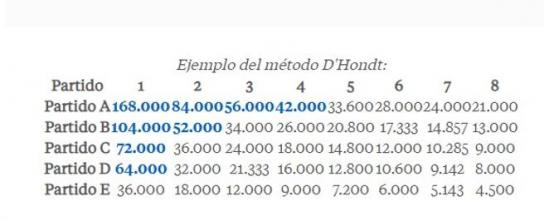
\includegraphics[width=1\linewidth]{graficos/vanguardia} 

}

\caption{Método D´Hondt}\label{fig:pressure}
\end{figure}

Es el sistema más habitualmente utilizado en las democracias actuales.
Utilizado en países como Albania, Argentina, Austria, Bélgica, Bolivia,
Brasil, Bulgaria, Camboya, Cabo Verde, Chile, Colombia, Croacia,
República Checa, República Dominicana, Ecuador, Escocia, Eslovenia,
España, Estonia, Finlandia, Gales, Guatemala, Hungría, Islandia, Israel,
Japón, Kosovo, Luxemburgo, Macedonia, Moldavia, Montenegro, Países
Bajos, Paraguay, Perú, Polonia, Portugal, Rumanía, Serbia, Timor del
Este, Turquía, Uruguay y parcialmente en Venezuela.

\hypertarget{reparto}{%
\subsubsection{Reparto}\label{reparto}}

Una vez escrutados la totalidad de los votos, se calculan cocientes
según la fórmula:

\(\textrm{Cociente} = \frac{V}{s+1}\) donde:

\(V\): Representa el número total de votos recibidos por la lista.

\(s\): Representa el número de escaños que cada lista se ha llevado de
momento, inicialmente 0 para cada lista.

El número de votos recibidos por cada lista se divide primero por 1,
después por 2, 3, hasta el número total de escaños para ese distrito. La
asignación de escaños se hace ordenando los cocientes de mayor a menor y
asignando a cada uno un escaño hasta que estos se agoten.

\hypertarget{muxe9todo-sainte-laguuxeb}{%
\subsection{Método Sainte-Laguë}\label{muxe9todo-sainte-laguuxeb}}

Método también conocido como método Webster, creado por el matemático
francés André Sainte-Laguë en 1832, similar al método D`Hondt. Es un
método de promedios mayores, utilizado en sistemas de votación
proporcional por listas.\\
El método de Sainte-Laguë es utilizado en una gran cantidad de países en
los que en la actualidad \footnote{Cierto a la fecha de realización del
  trabajo.} se encuentran, entre otros, estados como Noruega, Iraq y
Nueva Zelanda.

\hypertarget{reparto-1}{%
\subsubsection{Reparto}\label{reparto-1}}

Una vez escrutados la totalidad de los votos, se calculan cocientes
según la fórmula:

\(\textrm{Cociente} = \frac{V}{2s+1}\) donde:

\(V\): Representa el número total de votos recibidos por la lista.

\(s\): Representa el número de escaños que cada lista se ha llevado de
momento, inicialmente 0 para cada lista.

El número de votos recibidos por cada lista se divide sucesivamente por
cada uno de los valores que da la fórmula 2s+1 cuando s es igual a 0, 1,
2, 3, etc.; lo que supone dividir por 1, 3, 5, 7, etc. (es decir, la
sucesión de números impares). La asignación de escaños se hace ordenando
los cocientes de mayor a menor y asignando a cada uno un escaño hasta
que estos se agoten. A diferencia de otros sistemas, el número total de
votos no interviene en el cómputo.

\hypertarget{muxe9todo-sainte-laguuxeb-modificado}{%
\subsection{Método Sainte-Laguë
modificado}\label{muxe9todo-sainte-laguuxeb-modificado}}

Método utilizado en algunos países como Nepal o Suecia. Consiste en
utilizar una fórmula distinta para el primer escaño y a partir del
segundo utilizar el método habitual. Así, el método modificado cambia la
secuencia de divisores de (1, 3, 5, 7, \ldots) a (1.4, 3, 5, 7, \ldots).
Esto da una preferencia ligeramente mayor a los partidos más grandes
sobre los partidos más pequeños que ganarían, por un pequeño margen, un
solo escaño si se utilizara el método de Sainte-Laguë sin modificar. Con
el método modificado, estos partidos pequeños no obtienen
representación, en cambio, estos escaños se le otorgan a un partido más
grande. La forma para el primer escaño es:

\(\textrm{Cociente[s=0]} = \frac{V}{1.4}\) donde:

\(V\): Representa el número total de votos recibidos por la lista.

\hypertarget{muxe9todo-imperiali}{%
\subsection{Método Imperiali}\label{muxe9todo-imperiali}}

Otro método de promedio mayor se llama Imperiali (no debe confundirse
con la cuota Imperiali, que es un método del resto mayor). Los divisores
son 1, 1.5, 2, 2.5, 3, 3.5 y así sucesivamente. Está diseñado para
desfavorecer a los partidos más pequeños. Este método (a diferencia de
otros métodos enumerados) no es estrictamente proporcional, si es que
existe una asignación perfectamente proporcional, mediante este método
no se garantiza encontrarla. Método utilizado en Bélgica en las
elecciones municipales.\footnote{\emph{BJPS1992.pdf} ,
  \textless{}\url{https://www.tcd.ie/Political_Science/people/michael_gallagher/BJPS1992.pdf}\textgreater{}
  {[}accessed 4 May 2021{]}}

\hypertarget{muxe9todo-huntington-hill}{%
\subsection{Método Huntington-Hill}\label{muxe9todo-huntington-hill}}

Método creado en 1920 por Joseph Hill y corregido por el compañero de
escuela de Hill, Edward Huntington. Actualmente se utiliza para
distribuir los asientos que les corresponde a cada estado en la cámara
de representantes de los Estados Unidos de América. El objetivo es
mantener la relación de ``una persona un voto'' lo más cercana posible a
1.

\hypertarget{cuxe1lculo}{%
\subsubsection{Cálculo}\label{cuxe1lculo}}

Para distribuir los asientos entre los distintos partidos se utiliza el
divisor según \(\sqrt{n(n-1)}\). Los primeros divisores son 0, 1.41,
2.45, 3.46, 4.47. La asignación de escaños se hace ordenando los
cocientes de mayor a menor y asignando a cada uno un escaño hasta que
estos se agoten.

Para repartir los asientos por estado se utiliza el siguiente método:

I. Calculamos D:
\(\textrm{D} = \frac{Población Total}{NúmeroTotalDiputados}\)

\begin{enumerate}
\def\labelenumi{\Roman{enumi}.}
\setcounter{enumi}{1}
\tightlist
\item
  Calcular la cuota de diputados por estado:
\end{enumerate}

\(CoutaEstado = \frac{Población Estado}{D}\)

\begin{enumerate}
\def\labelenumi{\Roman{enumi}.}
\setcounter{enumi}{2}
\tightlist
\item
  Redondeamos la cuota a la parte entera.
\end{enumerate}

\(\textrm{n} = ParteEntera\left\{{Cuota Estado}\right\}\)

\begin{enumerate}
\def\labelenumi{\Roman{enumi}.}
\setcounter{enumi}{3}
\tightlist
\item
  Comparar la Cuota del estado con la media geométrica de \(n\) y
  \(n+1\), \(\sqrt{n(n+1)}\)
\end{enumerate}

Si
\(\begin{cases}CuotaEstado>MediaGeométrica & Representantes = n+1\\\textrm{Caso Contrario} & Representantes = n\end{cases}\)

Ajustar D para que el número de asientos totales coincida con el número
total de asientos designados.

\hypertarget{muxe9todo-danish}{%
\subsection{Método Danish}\label{muxe9todo-danish}}

El método danés\footnote{Wikipedia contributors, `Highest averages
  method', \emph{Wikipedia, The Free Encyclopedia,} 31 December 2020,
  20:02 UTC,
  \textless{}\url{https://en.wikipedia.org/w/index.php?title=Highest_averages_method\&oldid=997495824}\textgreater{}
  {[}accessed 4 May 2021{]}} se utiliza en las elecciones danesas para
asignar los escaños de cada partido a nivel de provincia electoral.
Divide el número de votos recibidos por un partido en una
circunscripción de varios miembros por los divisores que aumentan de
tres en tres (1, 4, 7, 10, etc.). También, dividir los números de votos
por 0.33, 1.33, 2.33, 3.33, etc. da el mismo resultado. Este sistema
intenta deliberadamente asignar escaños por igual en lugar de
proporcionalmente.

\hypertarget{muxe9todo-adams}{%
\subsection{Método Adams}\label{muxe9todo-adams}}

El método de Adams fue concebido por John Quincy Adams para distribuir
los escaños de la Cámara entre los distintos estados. Otorga un escaño
al partido que tiene más votos por escaño antes de que se agregue el
escaño.

El método de Adams usa \(n-1\) como divisor. La secuencia de los cinco
primeros divisores serían (0,1,2,3,4). Al igual que el método
Huntington-Hill, esto da como resultado un valor de 0 para los primeros
escaños que se designarán para cada partido, lo que da como resultado un
promedio de \(\infty\).

Sin umbral, todos los partidos que han recibido al menos un voto,
también reciben un escaño, con la obvia excepción de los casos en los
que hay más partidos que escaños. Esta propiedad puede ser deseable, por
ejemplo, al distribuir escaños entre distritos electorales. Siempre que
haya al menos tantos escaños como distritos, todos los distritos estarán
representados. En una elección de representación proporcional por lista
de partidos, puede resultar en que partidos muy pequeños obtengan
escaños. Las violaciones de la regla de la cuota en el método puro de
Adams son muy comunes. Estos problemas pueden resolverse mediante la
introducción de un umbral electoral.

\hypertarget{muxe9todo-del-resto-mayor}{%
\section{Método del resto mayor}\label{muxe9todo-del-resto-mayor}}

Es un método para distribuir los escaños proporcionalmente para un
sistema de listas de partidos. Son una alternativa a los métodos de
promedio mayor.

El método del resto mayor requiere que el número de votos de cada
partido se divida por una cuota que represente el número de votos
necesarios para un escaño (es decir, normalmente el número total de
votos emitidos dividido por el número de escaños, o alguna fórmula
similar). El resultado para cada partido consistirá normalmente en la
parte entera más un resto. A cada partido se le asigna primero un número
de escaños igual a su número entero. Esto generalmente dejará algunos
escaños sin asignar: los partidos se clasificarán entonces sobre la base
de los restos, y a los partidos con los restos más grandes se les asigna
cada uno un escaño adicional hasta que se hayan asignado todos los
escaños. De ahí el nombre del método. Hay distintos modelos para
calcular el cociente, los más utilizados son el cociente Hare, Droop e
Imperiali.

\hypertarget{cociente-droop}{%
\subsection{Cociente Droop}\label{cociente-droop}}

Algunos países que emplean este cociente son Australia Irlanda o Malta,
entre otros. Es más favorable a los partidos mayoritarios que el
obtenido mediante el sistema Hare, aunque no favorece tanto como el
sistema Imperiali.

Si se eligen \({n}\) escaños para un cuerpo colegiado, y se emiten
\({m}\) votos válidos, se establece un cociente \({q}\) el cual
utilizaremos para repartir los votos. Este cociente se calcula mediante
la fórmula:

\({q=1+{\frac {m}{n+1}}}\) con \(q\) aproximado al entero más próximo.

Si la i-ésima lista de I listas inscritas obtiene \({m_{i}}\) votos,
esta lista tendrá \({e_{i}}\) escaños por cociente y \({r_{i}}\) votos
por residuo mediante la fórmula: \({m_{i}=qe_{i}+r_{i}}\)

\({e_{i}=\left\lfloor {\frac {m_{i}}{q}}\right\rfloor ,r_{i}=m_{i}-qe_{i}}\)

Definimos k como el número de escaños restantes que no son obtenidos por
el cociente:

\({k=n-\sum _{i=1}^{I}e_{i}}\)

Estos k escaños son repartidos entre los mejores k residuos \({r_{i}}\).

De esta forma, el número total de escaños del i-ésimo partido será
\({p_{i}=e_{i}}\) o \({p_{i}=e_{i}+1}\).

\hypertarget{cociente-hare}{%
\subsection{Cociente Hare}\label{cociente-hare}}

La fórmula del cociente Hare es la fórmula más simple que puede
utilizarse en unas elecciones según un sistema de voto transferible
único, también se utiliza en sistemas de representación proporcional por
listas. En comparación con algunos métodos similares, la utilización del
método del cociente de Hare con el método de resto mayor tiende a
favorecer a las partes más pequeñas a expensas de las más grandes.

\begin{itemize}
\item
  Fórmula:

  El cociente se calcula mediante la siguiente fórmula y se siguen los
  pasos explicados anteriormente para el cociente Droop:
\end{itemize}

\(Cociente = \frac{Total Votos}{Total Escaños}\)

\hypertarget{cociente-imperiali}{%
\subsection{Cociente Imperiali}\label{cociente-imperiali}}

El reparto es más favorable a los partidos mayoritarios que el que se
pueda obtener mediante los métodos de Hare o Droop.

\begin{itemize}
\tightlist
\item
  Reparto
\end{itemize}

Si se eligen n escaños para un cuerpo colegiado, y se emiten m votos
válidos, se establece un cociente q el cual servirá para repartir los
votos. Este cociente se calcula mediante la fórmula:

\({q={\frac {m}{n+2}}}\) con q aproximado al entero más próximo.

Si la i-ésima lista de I listas inscritas obtiene \({m_{i}}\) votos,
esta lista tendrá \({e_{i}}\) escaños por cociente y \({r_{i}}\) votos
por residuo mediante la fórmula: \({m_{i}=qe_{i}+r_{i}}\).

\({e_{i}=\left\lfloor {\frac {m_{i}}{q}}\right\rfloor ,r_{i}=m_{i}-qe_{i}}\)

\hypertarget{otros-muxe9todos}{%
\section{Otros métodos}\label{otros-muxe9todos}}

\hypertarget{muxe9todo-de-condorcet}{%
\subsection{Método de Condorcet}\label{muxe9todo-de-condorcet}}

El método de Condorcet lleva el nombre del matemático y filósofo francés
del siglo XVIII Marie Jean Antoine Nicolas Caritat, marqués de
Condorcet, aunque anteriormente Ramón Llull en 1299 creó un método
similar que cumple el criterio de Condorcet pero en un diseño iterativo.
Actualmente este método no se utiliza en ningún país.

Es uno de los métodos en los que se elige al candidato que gana la
mayoría de los votos en cada par de elecciones frente a cada uno de los
otros candidatos, es decir, un candidato preferido por más votantes que
cualquier otro, siempre que exista tal candidato. Un candidato con esta
propiedad, el campeón de la pareja o el ganador de la victoria, se llama
formalmente el ganador de Condorcet.

Puede que no siempre exista un ganador del premio Condorcet en una
elección particular porque la preferencia de un grupo de votantes que
seleccionan entre más de dos opciones puede ser cíclica, es decir, es
posible (pero muy raro) que cada candidato tenga un oponente que le
derrote en una contienda entre dos candidatos. La posibilidad de tales
preferencias cíclicas en un grupo de votantes se conoce como la paradoja
de Condorcet.

\hypertarget{procedimiento}{%
\subsubsection{Procedimiento}\label{procedimiento}}

\begin{itemize}
\item
  Voto\\
  En una elección según el método de Condorcet el votante rellena la
  lista de candidatos por orden de preferencia.
\item
  Vencedor\\
  El recuento se realiza contrastando a cada candidato contra todos los
  demás candidatos en una serie de hipotéticos enfrentamientos uno a
  uno. El ganador de cada pareja es el candidato preferido por la
  mayoría de los votantes. Se considera que el candidato preferido por
  cada votante es el que está más alto en su papeleta de votación.
  Cuando se han considerado todos los emparejamientos posibles de
  candidatos, si un candidato vence a todos los demás candidatos en
  estos concursos, entonces se le declara ganador de Condorcet. Como se
  ha señalado anteriormente, si no hay un ganador de Condorcet debe
  utilizarse otro método para encontrar el ganador de la elección, y
  este mecanismo varía de un método de Condorcet a otro.
\item
  Recuento de votos mediante matrices\\
  Se utiliza para los resultados una matriz en donde cada fila es el
  elemento como ``contendiente'' y en cada columna el elemento como
  ``oponente''.

  En el caso de que un candidato gane a todos los restantes, será el
  ganador de Condorcet. Cuando no hay un ganador Condorcet se utilizan
  métodos alternativos de Condorcet, como el método Minimax y el método
  Schulze, que utilizan la información contenida en la matriz para
  elegir un ganador.
\end{itemize}

\hypertarget{muxe9todo-schulze}{%
\subsection{Método Schulze}\label{muxe9todo-schulze}}

Método por el cual se selecciona un ganador a partir de las preferencias
de los votantes, fue creado en 1997 por Markus Schulze.

\begin{itemize}
\item
  Método

  \begin{itemize}
  \tightlist
  \item
    Averiguar el conjunto de Schwartz (el menor conjunto de candidatos
    que no es ganado por nadie fuera del conjunto). Si sólo hay un
    candidato en el conjunto, este es el ganador de Condorcet. Si hay
    varios miembros pero no hay derrotas entre ellos, entonces hay un
    empate normal entre ellos.
  \item
    En cualquier otro caso, eliminar la derrota más suave en el conjunto
    de Schwartz (es decir, aquella ganada por el menor margen).
    Recalcular el nuevo conjunto de Schwartz y repetir el proceso.
  \end{itemize}
\end{itemize}

\hypertarget{regla-de-hamilton}{%
\subsection{Regla de Hamilton}\label{regla-de-hamilton}}

El Método de Hamilton es un método que se emplea para repartir los
escaños de un Parlamento. Se trata de un método no proporcional, ya que
dependiendo de la provincia se necesitará un número diferente de votos
para obtener un escaño.

Para conseguir que cada estado recibiera un número de representantes lo
más cercano a su cuota, Hamilton asigna a cada estado, en una primera
aproximación, la parte entera de su cuota. Luego, los escaños aún no
repartidos se reparten por orden de mayor a menor a los que tienen parte
decimal más grande.

\(\textrm{Cuota} = \frac{Censo Distrito}{Censo Total}\)

\FloatBarrier

\ifdefined\ifprincipal
\else
\setlength{\parindent}{1em}
\pagestyle{fancy}
\setcounter{tocdepth}{4}
\tableofcontents

\fi

\ifdefined\ifdoblecara
\fancyhead{}{}
\fancyhead[LE,RO]{\scriptsize\rightmark}
\fancyfoot[LO,RE]{\scriptsize\slshape \leftmark}
\fancyfoot[C]{}
\fancyfoot[LE,RO]{\footnotesize\thepage}
\else
\fancyhead{}{}
\fancyhead[RO]{\scriptsize\rightmark}
\fancyfoot[LO]{\scriptsize\slshape \leftmark}
\fancyfoot[C]{}
\fancyfoot[RO]{\footnotesize\thepage}
\fi
\renewcommand{\headrulewidth}{0.4pt}
\renewcommand{\footrulewidth}{0.4pt}

\hypertarget{anuxe1lisis-de-los-muxe9todos-de-reparto-de-escauxf1os}{%
\chapter{Análisis de los métodos de reparto de
escaños}\label{anuxe1lisis-de-los-muxe9todos-de-reparto-de-escauxf1os}}

En este bloque simularemos distintos escenarios para analizarlos según
los distintos métodos de reparto de escaños.

Los sistemas que analizaremos en este análisis serán, dentro de los
métodos de promedio mayor, el método \emph{D´Hondt}, método
\emph{Saint-Lague}, método \emph{Saint-Lague modificado}, el método
\emph{Huntington-Hill}, el método \emph{Imperiali}, \emph{Danish} y
\emph{Adams}. Dentro de los métodos de resto mayor analizaremos el
método \emph{Droop}, \emph{Hare} e \emph{Imperiali}.

\hypertarget{procedimiento-general}{%
\section{Procedimiento general}\label{procedimiento-general}}

Generaremos datos ficticios de partidos, utilizaremos tres distintas
variables, que son el número de partidos, el número de escaños a
repartir y la concentración del voto entre los partidos. De estas tres
variables dejaremos dos variables fijas y una tercera que irá variando:

\begin{itemize}
\item
  La variable \emph{número de partidos} variará entre los 2 posibles
  partidos hasta los 100 partidos, por ejemplo en países como la India
  podemos observar que se presentan a las elecciones hasta 2698
  partidos, aunque no todos ellos de nivel estatal. En el caso de que la
  variable quede fija el valor por defecto serán 20 partidos.
\item
  La variable \emph{número de escaños} variará entre el reparto de 1
  sólo escaño hasta 800 escaños, números similares de escaños a repartir
  podemos observarlos en Reino Unido o más aún escaños, hasta 2987 en
  China. En el caso de que la variable quede fija el valor por defecto
  serán 350 escaños.
\item
  La variable \emph{concentración del voto} varía entre una casi máxima
  igualdad de votos entre partidos, es decir, que casi no hay diferencia
  de votos entre los distintos partidos, hasta una desigualdad muy
  marcada de los votos que reciben cada partido. En el caso de que la
  variable quede fija el valor por defecto será una concentración del
  voto de nivel medio. Como ejemplo presentamos un gráfico para que sea
  más comprensivo:
\end{itemize}

\begin{center}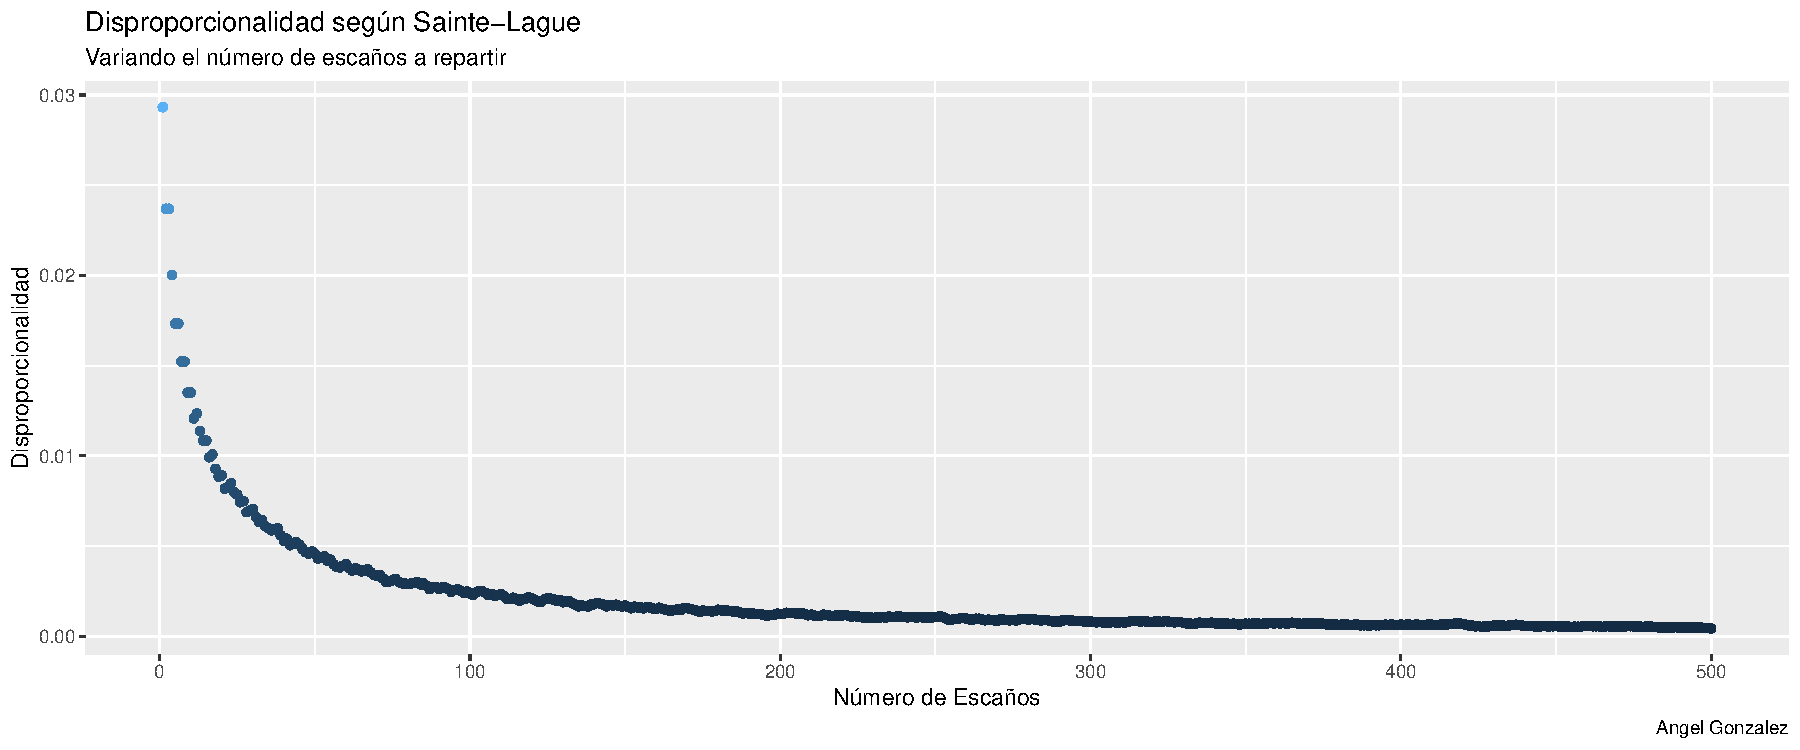
\includegraphics[width=0.95\linewidth]{figurasR/unnamed-chunk-14-1} \end{center}

\hypertarget{cuxe1lculo-de-la-desproporciuxf3n}{%
\section{Cálculo de la
desproporción}\label{cuxe1lculo-de-la-desproporciuxf3n}}

En este bloque los resultados son comparados mediante un índice que
calcula la desproporción, que mide cuánto de los votos que obtienen los
partidos se traducen a representación en escaños. A continuación
presentaremos la función y explicaremos el procedimiento de cálculo:

\begin{Shaded}
\begin{Highlighting}[]
\NormalTok{desproporción }\OtherTok{\textless{}{-}}
  \ControlFlowTok{function}\NormalTok{(s, v) \{  }\CommentTok{\# Variables}
\NormalTok{    s }\OtherTok{\textless{}{-}} \FunctionTok{as.vector}\NormalTok{(s)}
\NormalTok{    v }\OtherTok{\textless{}{-}} \FunctionTok{as.vector}\NormalTok{(v)}
\NormalTok{    l\_s }\OtherTok{\textless{}{-}} \FunctionTok{length}\NormalTok{(s)}
    \CommentTok{\# Suma de escaños y votos}
\NormalTok{    s\_s }\OtherTok{\textless{}{-}} \FunctionTok{sum}\NormalTok{(s)   }
\NormalTok{    s\_v }\OtherTok{\textless{}{-}} \FunctionTok{sum}\NormalTok{(v)}
    \CommentTok{\# Dividir escaños y votos entre sus totales}
\NormalTok{    p\_s }\OtherTok{\textless{}{-}}\NormalTok{ s }\SpecialCharTok{/}\NormalTok{ s\_s}
\NormalTok{    p\_v }\OtherTok{\textless{}{-}}\NormalTok{ v }\SpecialCharTok{/}\NormalTok{ s\_v}
    \CommentTok{\# Aplicar la fórmula para obtener la desproporción}
\NormalTok{    o }\OtherTok{\textless{}{-}}\NormalTok{ (}\DecValTok{1} \SpecialCharTok{/}\NormalTok{ l\_s) }\SpecialCharTok{*} \FunctionTok{sum}\NormalTok{(}\FunctionTok{abs}\NormalTok{(p\_s }\SpecialCharTok{{-}}\NormalTok{ p\_v))}
\NormalTok{    o}
\NormalTok{  \}}
\end{Highlighting}
\end{Shaded}

\begin{itemize}
\tightlist
\item
  La función depende de dos variables:

  \begin{itemize}
  \tightlist
  \item
    \emph{s}: Escaños obtenidos por cada partido.
  \item
    \emph{v}: Votos obtenidos por cada partido.
  \end{itemize}
\item
  En primer lugar se realiza la suma total de escaños, que se recoge en
  la variable \emph{s\_s} y la suma total de votos, recogida en la
  variable \emph{s\_v}.
\item
  A continuación para cada partido se dividen los escaños obtenidos
  entre el total de escaños a repartir, se recoge en la variable
  \emph{p\_s}. El mismo procedimiento para los votos, para cada partido
  se dividen los votos obtenidos entre el total de votos, recogido en la
  variable \emph{p\_v}.
\item
  Finalmente para cada partido se restan los resultados \emph{p\_s} y
  \emph{p\_v} anteriormente obtenidos, seguidamente nos quedamos con el
  valor absoluto de los resultados, sumamos todos los valores y los
  dividimos entre el número de partidos, lo recogemos en la variable
  \emph{o}.
\end{itemize}

Los valores sobre los que puede variar la función de desproporción
parten de 0, que representaría una proporcionalidad perfecta, y cuanto
mayor vaya siendo el valor obtenido, peor proporcionalidad presentará.
Por lo tanto para un método de reparto deseable lo que se pretende
conseguir es presentar el mínimo valor posible, cuanto menor valor de
desproporción obtenga mejor método será.

\hypertarget{dhondt}{%
\section{D`Hondt}\label{dhondt}}

\hypertarget{dhondt-variando-el-nuxfamero-de-escauxf1os}{%
\subsection{D`Hondt variando el número de
escaños}\label{dhondt-variando-el-nuxfamero-de-escauxf1os}}

\begin{center}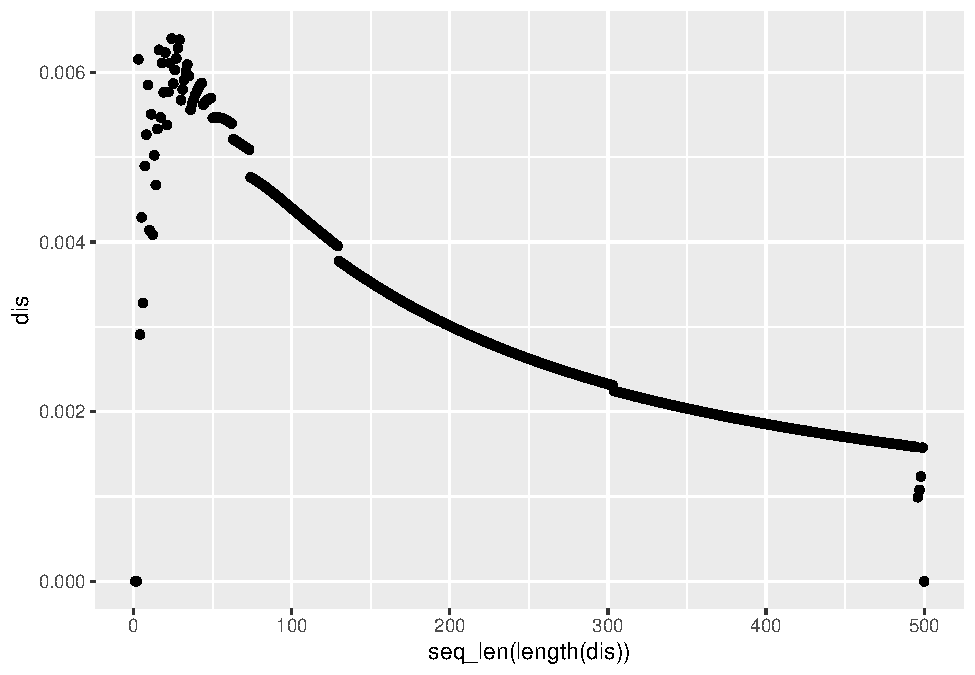
\includegraphics[width=0.95\linewidth]{figurasR/unnamed-chunk-18-1} \end{center}

En este caso se nos presenta la desproporción variando el número de
escaños posibles, se empieza por repartir un único escaño hasta los 800
posibles escaños. Observamos que la desproporción en el caso de un
escaño es relativamente alta, posteriormente cuanto mayor es el número
de escaños a repartir la desproporción va bajando hasta casi alcanzar la
perfección deseada de un valor de la desproporción de 0.\\
La diferencia de desproporción entre los casos en los que hay pocos
escaños a repartir es alta, cuantos mas escaños a repartir la diferencia
de desproporción entre sucesivos escaños se va reduciendo, a números
altos de escaños a repartir la desproporción tiende a estabilizarse.\\
Para este caso apreciamos que a partir de los 50-100 escaños ya la
desproporción es muy baja, siendo recomendable la utilización de un
número de escaños a partir de los 300.

\hypertarget{dhondt-variando-el-nuxfamero-de-partidos}{%
\subsection{D`Hondt variando el número de
partidos}\label{dhondt-variando-el-nuxfamero-de-partidos}}

\begin{center}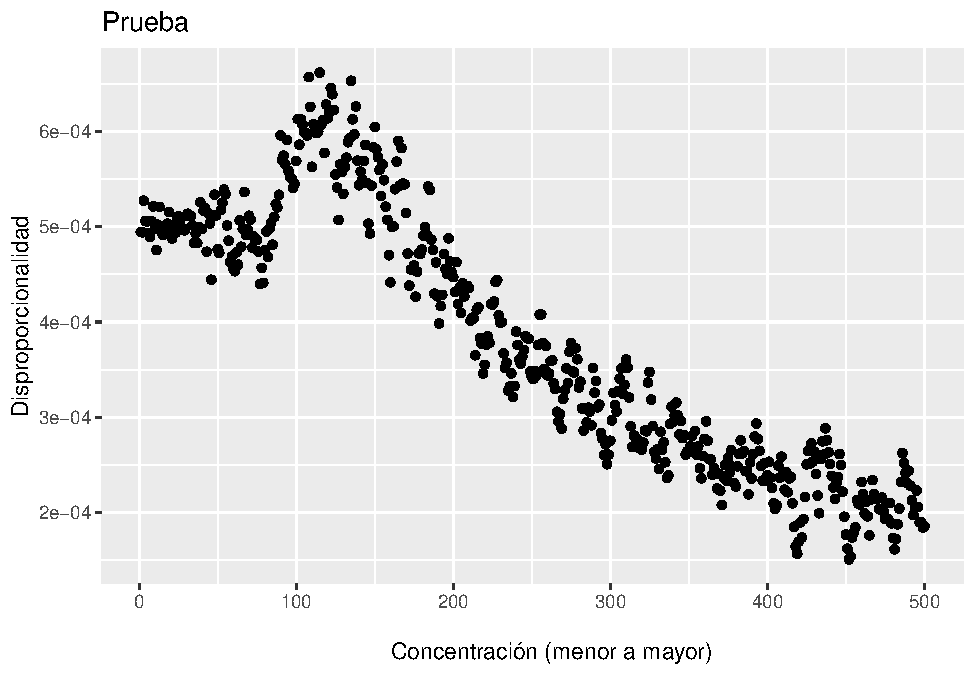
\includegraphics[width=0.95\linewidth]{figurasR/unnamed-chunk-19-1} \end{center}

En este caso únicamente modificamos el número de partidos presentes en
la elección, desde un único partido hasta 100 partidos que se presentan
a una elección ficticia. Observamos que cuando se presentan de 2 a 12
partidos a las elecciones la desproporción es media, va aumentando a
medida que se presentan más partidos, alcanzando el máximo de
desproporción alrededor de los 25 partidos que se presentan a las
elecciones, a partir de ese punto la curva comienza a decrecer.\\
Podemos apreciar en el gráfico que para un número bajo de partidos que
se presentan a las elecciones ( de 2 a 12 ) la desproporción es media,
levemente creciente y con una gran variabilidad, a partir de los 12
partidos la variabilidad de un punto al siguiente se estabiliza con una
variabilidad decreciente cuantos más partidos entren en la elección.

\hypertarget{dhondt-variando-la-concentraciuxf3n-del-voto}{%
\subsection{D`Hondt variando la concentración del
voto}\label{dhondt-variando-la-concentraciuxf3n-del-voto}}

\begin{center}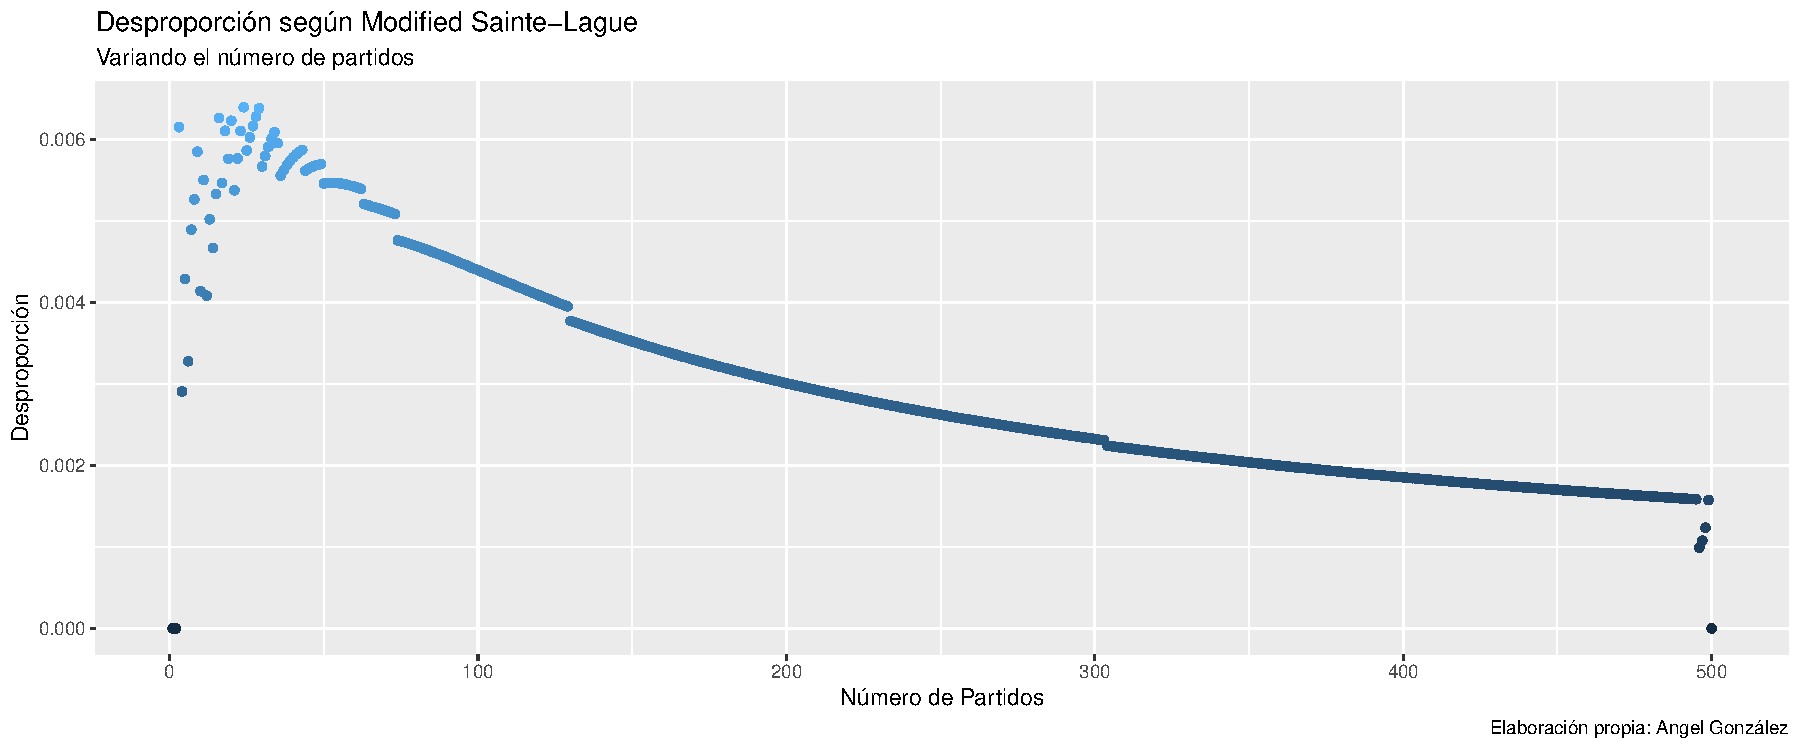
\includegraphics[width=0.95\linewidth]{figurasR/unnamed-chunk-20-1} \end{center}

En el presente gráfico variamos la concentración del voto en unas
elecciones ficticias, comenzamos con una concentración de votos baja, es
decir, la diferencia de votos entre partidos es baja, hasta acabar con
una concentración de votos alta, en donde la diferencia de votos entre
partidos es muy grande.\\
Observando el gráfico apreciamos que cuando la concentración del voto es
muy baja la desproporción está también en un nivel bajo, cuanto más
concentración del voto en pocos partidos comprobamos como la
desproporción aumenta, hasta que alcanza un punto en donde alcanza el
máximo de desproporción, que sería un punto de concentración de los
votos entre partidos media-alta y a partir de ese punto la desproporción
va bajando cuanta mayor diferencia de votos se presente entre los
partidos.\\
Así podemos concluir que el reparto de escaños según la ley D`Hondt es
mejor cuanto más concentración de voto tengan unos pocos partidos con
respecto a los demás o bien cuando haya poca diferencia de votos entre
los partidos.

\hypertarget{sainte-lague}{%
\section{Sainte-Lague}\label{sainte-lague}}

\hypertarget{sainte-lague-variando-el-nuxfamero-de-escauxf1os}{%
\subsection{Sainte-Lague variando el número de
escaños}\label{sainte-lague-variando-el-nuxfamero-de-escauxf1os}}

\begin{center}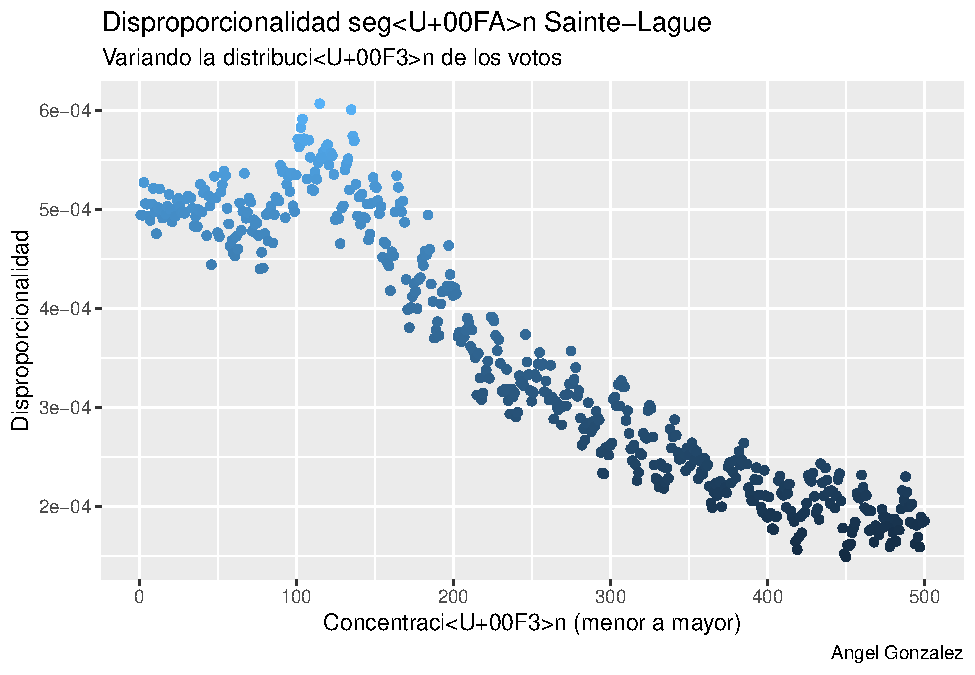
\includegraphics[width=0.95\linewidth]{figurasR/unnamed-chunk-23-1} \end{center}

En este caso se nos presenta la desproporción variando el número de
escaños posibles, se empieza por repartir un único escaño hasta los 800
posibles escaños. Observamos que la desproporción en el caso de un
escaño es muy alta, posteriormente cuanto mayor es el número de escaños
a repartir la desproporción va bajando. La diferencia de desproporción
en los casos en los que hay pocos escaños a repartir es alta, cuantos
mas escaños a repartir la diferencia de desproporción entre sucesivos
escaños va reduciéndose, a partir de los 50 escaños es aceptable la
desproporción aunque sería deseable partir de los 200 escaños.

\hypertarget{sainte-lague-variando-el-nuxfamero-de-partidos}{%
\subsection{Sainte-Lague variando el número de
partidos}\label{sainte-lague-variando-el-nuxfamero-de-partidos}}

\begin{center}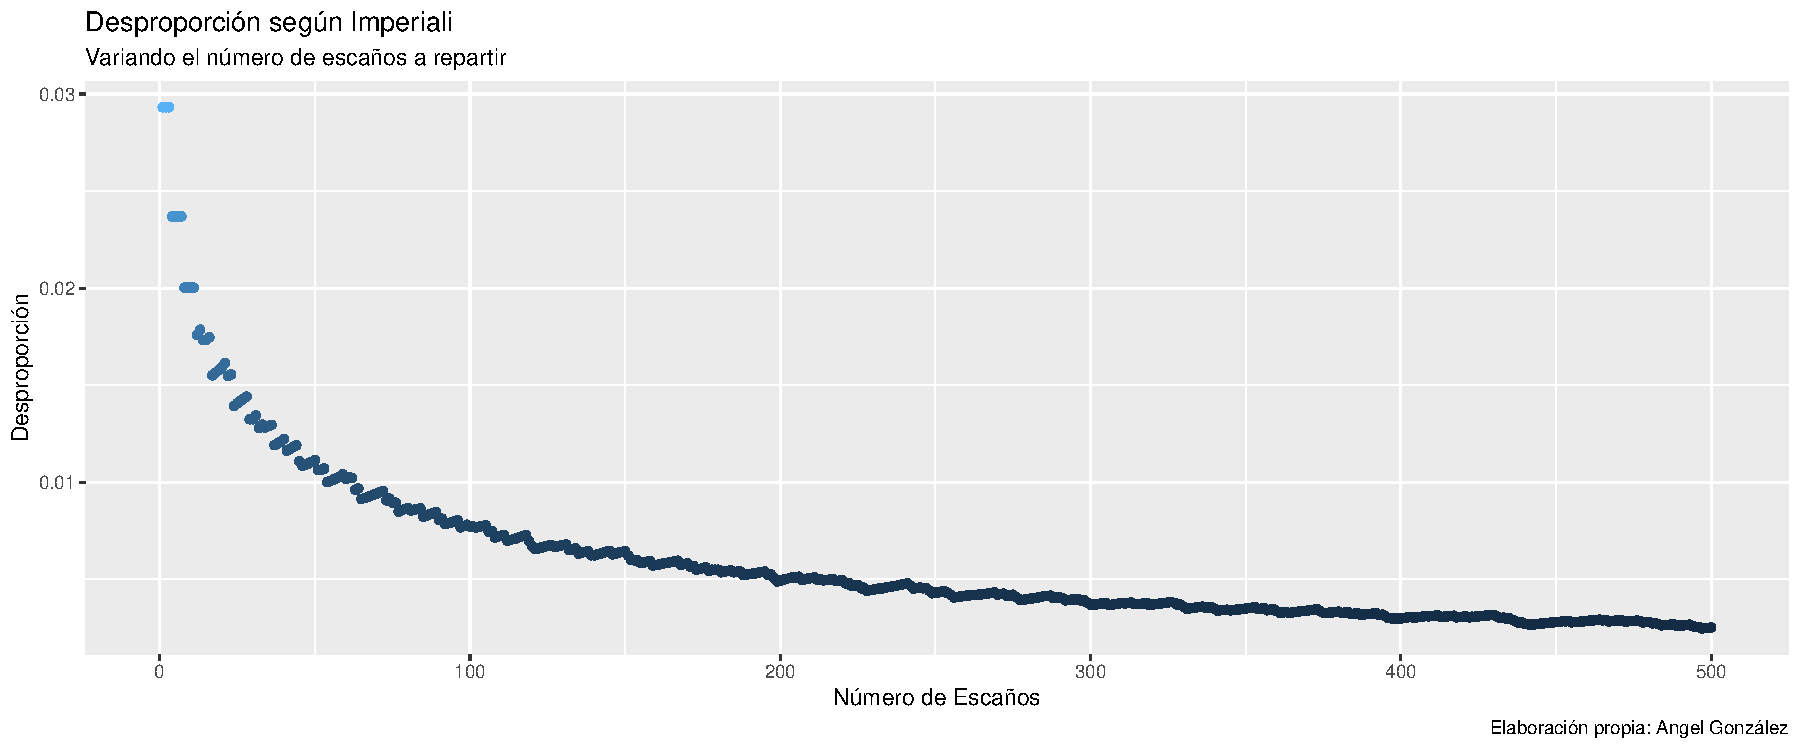
\includegraphics[width=0.95\linewidth]{figurasR/unnamed-chunk-24-1} \end{center}

En este caso únicamente modificamos el número de partidos presentes en
la elección, desde un único partido hasta 100 partidos que se presentan
a una elección ficticia. Observamos que cuando se presentan 2 partidos a
las elecciones la desproporción empieza siendo alta, queda en un mismo
nivel a medida que se presentan más partidos, alcanzando el máximo de
desproporción con 25 partidos que se presentan a las elecciones, a
partir de ese punto la curva desciende constantemente alcanzando cotas
de desproporción muy deseables. Podemos apreciar en el gráfico que para
un número de 2 a 25 partidos que se presentan a las elecciones la
desproporción es alta y presenta mucha variabilidad, a partir de los 26
partidos, cuanto mayor número de partidos se presenten en las elecciones
menor va a ser la variabilidad que encontremos.

\hypertarget{sainte-lague-variando-la-concentraciuxf3n-del-voto}{%
\subsection{Sainte-Lague variando la concentración del
voto}\label{sainte-lague-variando-la-concentraciuxf3n-del-voto}}

\begin{center}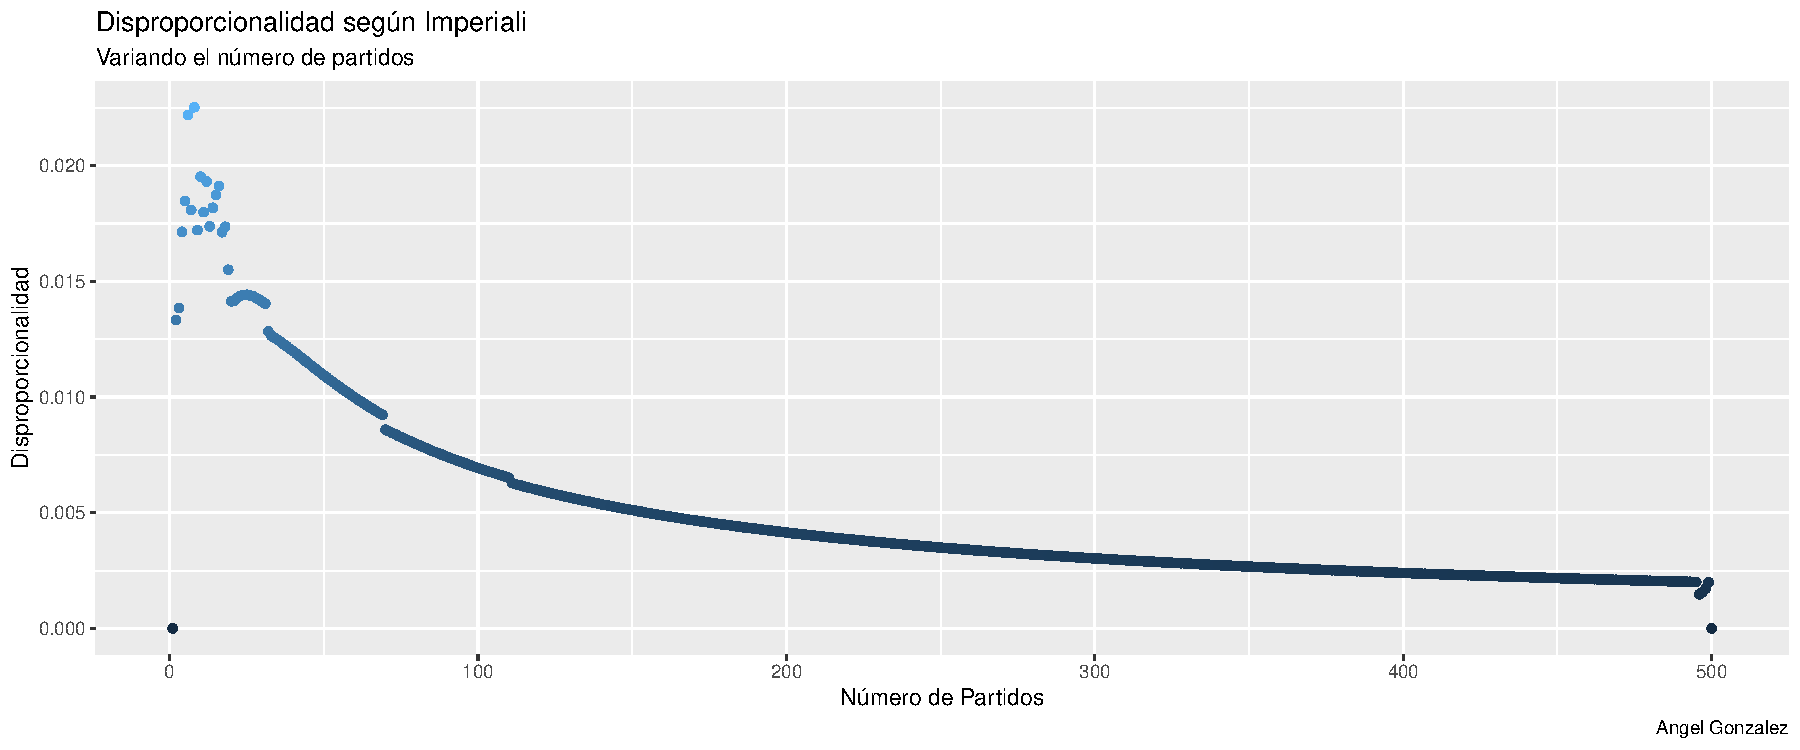
\includegraphics[width=0.95\linewidth]{figurasR/unnamed-chunk-25-1} \end{center}

En el presente gráfico variamos la concentración del voto en unas
elecciones ficticias, comenzamos con una concentración de votos baja, es
decir, la diferencia de votos entre partidos es baja, hasta acabar con
una concentración de votos alta, en donde la diferencia de votos entre
partidos es muy grande. En este método de Sainte-Lague la desproporción
es especialmente baja, característica muy deseable, además no se
aprecian diferencias de desproporción en casos de poca a alta
concentración del voto, la variabilidad que apreciamos en la gráfica es
alta pero teniendo en cuenta el rango en que se mueve podemos decir que
la variabilidad es baja sea cual sea la concentración del voto.

\hypertarget{modified-sainte-lague}{%
\section{Modified Sainte-Lague}\label{modified-sainte-lague}}

\hypertarget{modified-sainte-lague-variando-el-nuxfamero-de-escauxf1os}{%
\subsection{Modified Sainte-Lague variando el número de
escaños}\label{modified-sainte-lague-variando-el-nuxfamero-de-escauxf1os}}

\begin{center}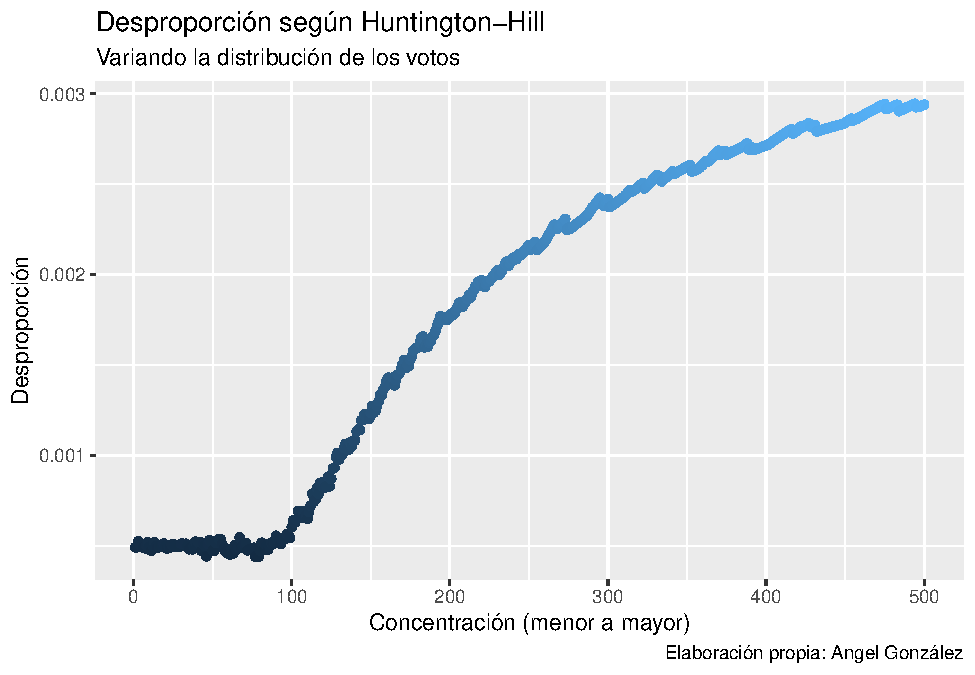
\includegraphics[width=0.95\linewidth]{figurasR/unnamed-chunk-28-1} \end{center}

En este caso se nos presenta la desproporción variando el número de
escaños posibles, en el presente caso se empieza por repartir un único
escaño hasta los 800 posibles escaños. Observamos que la desproporción
en el caso de un escaño es muy alta, posteriormente cuanto mayor es el
número de escaños a repartir la desproporción va bajando. La diferencia
que encontramos de desproporción entre los casos en los que hay pocos
escaños a repartir es alta, cuantos mas escaños a repartir la diferencia
de desproporción entre sucesivos escaños va reduciéndose, a números
altos de escaños a repartir la desproporción tiende a estabilizarse. En
este método también empieza a ser aceptable escoger un número de escaños
igual o mayor a 50 escaños.

\hypertarget{modified-sainte-lague-variando-el-nuxfamero-de-partidos}{%
\subsection{Modified Sainte-Lague variando el número de
partidos}\label{modified-sainte-lague-variando-el-nuxfamero-de-partidos}}

\begin{center}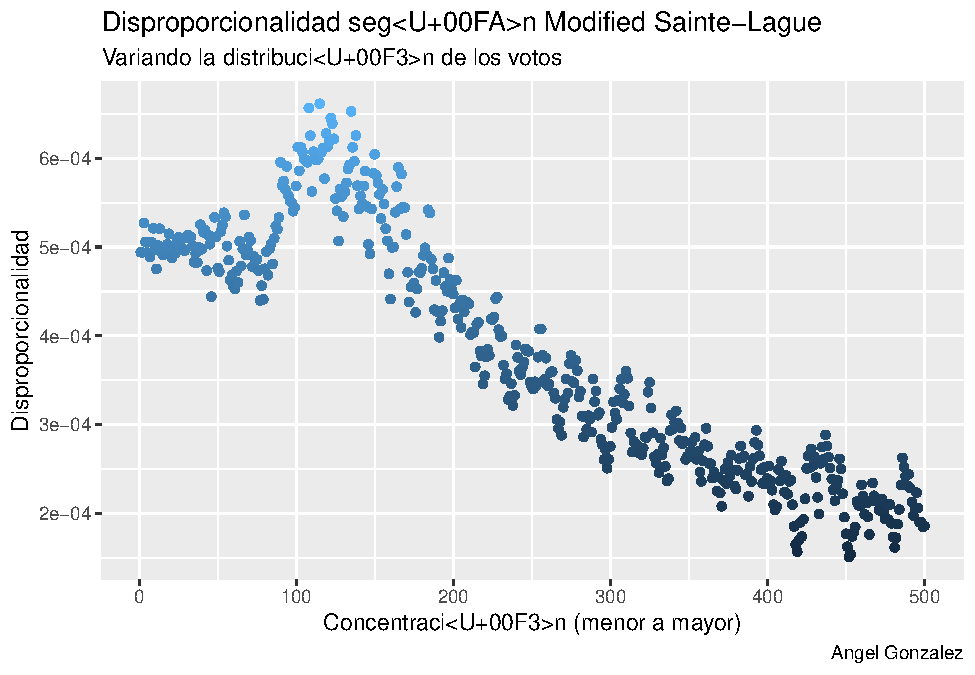
\includegraphics[width=0.95\linewidth]{figurasR/unnamed-chunk-29-1} \end{center}

En este caso únicamente modificamos el número de partidos presentes en
la elección, desde un único partido hasta 100 partidos que se presentan
a una elección ficticia. Observamos que cuando se presentan de 2 a 20
partidos a las elecciones la desproporción es media, va aumentando a
medida que se presentan más partidos, alcanzando el máximo de
desproporción alrededor de los 28 partidos que se presentan a las
elecciones, número del cual la curva comienza a decrecer. Podemos
apreciar en el gráfico que para un número bajo de partidos que se
presentan a las elecciones la varianza es alta, a partir de ese número
de partidos la diferencia entre los siguientes puntos va reduciéndose
paulatinamente cuanto mayor número de partidos concurran a las
elecciones ficticias.

\hypertarget{modified-sainte-lague-variando-la-concentraciuxf3n-del-voto}{%
\subsection{Modified Sainte-Lague variando la concentración del
voto}\label{modified-sainte-lague-variando-la-concentraciuxf3n-del-voto}}

\begin{center}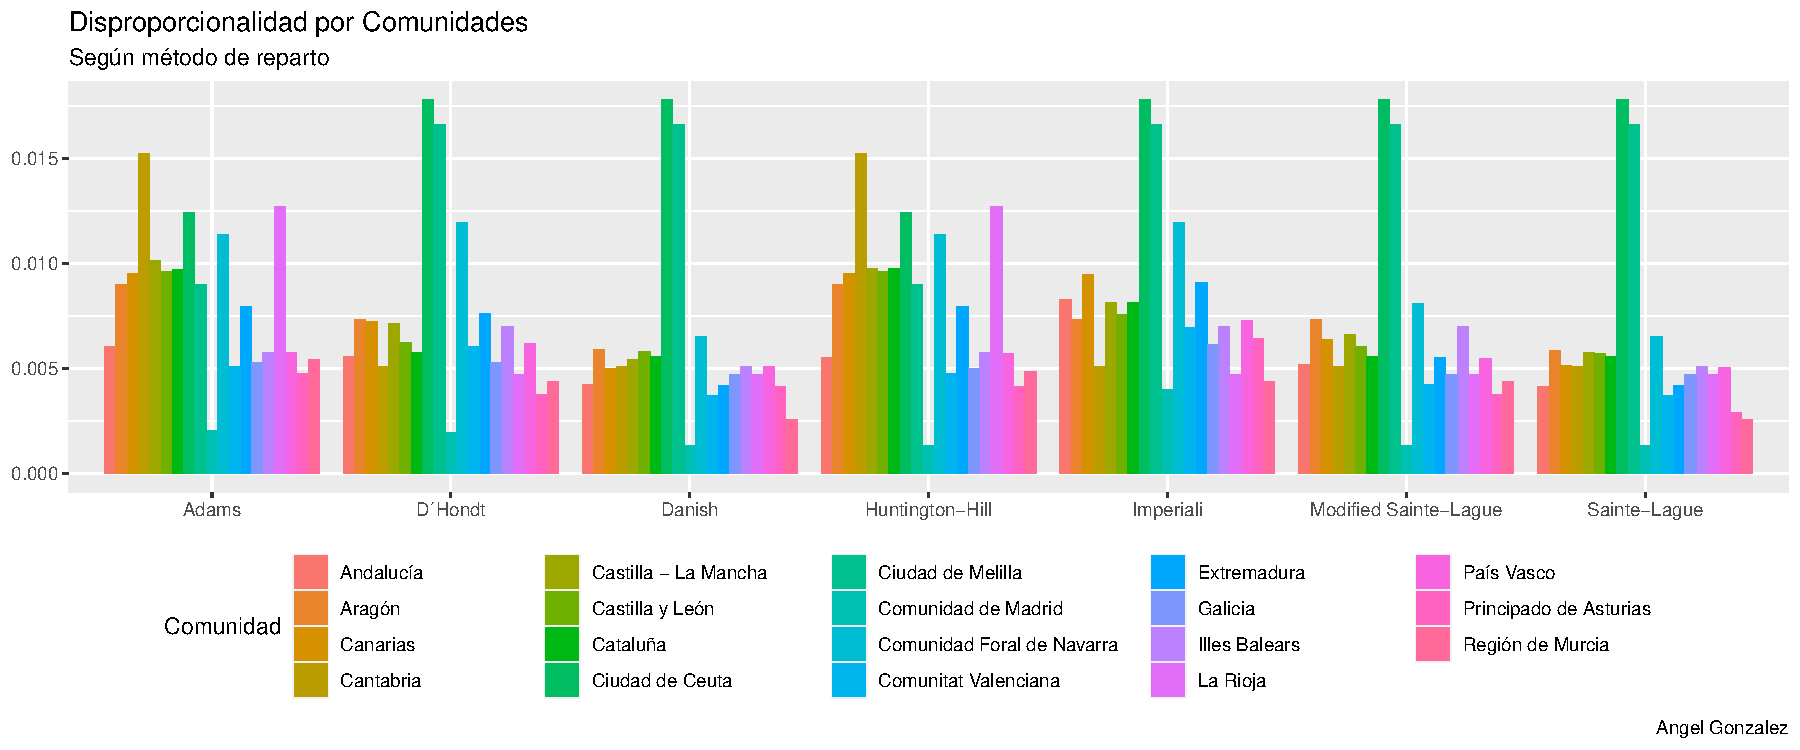
\includegraphics[width=0.95\linewidth]{figurasR/unnamed-chunk-30-1} \end{center}

En el presente gráfico variamos la concentración del voto en unas
elecciones ficticias, comenzamos con una concentración de votos baja, es
decir, la diferencia de votos entre partidos es baja, hasta acabar con
una concentración de votos alta, en donde la diferencia de votos entre
partidos es muy grande.\\
Observando el gráfico observamos que la desproporción, tal y como
sucedía con el método Sainte-Lague, es muy baja, manteniéndose en una
misma franja ya sea la concentración del voto entre los partidos alta o
baja.\\
Así podemos concluir que el reparto de escaños según la ley Modified
Sainte-Lague en este caso presenta unas cualidades muy deseables, tiene
un nivel de desproporción muy bajo y no depende significativamente del
nivel de la concentración del voto entre los partidos.

\hypertarget{imperiali}{%
\section{Imperiali}\label{imperiali}}

\hypertarget{imperiali-variando-el-nuxfamero-de-escauxf1os}{%
\subsection{Imperiali variando el número de
escaños}\label{imperiali-variando-el-nuxfamero-de-escauxf1os}}

\begin{center}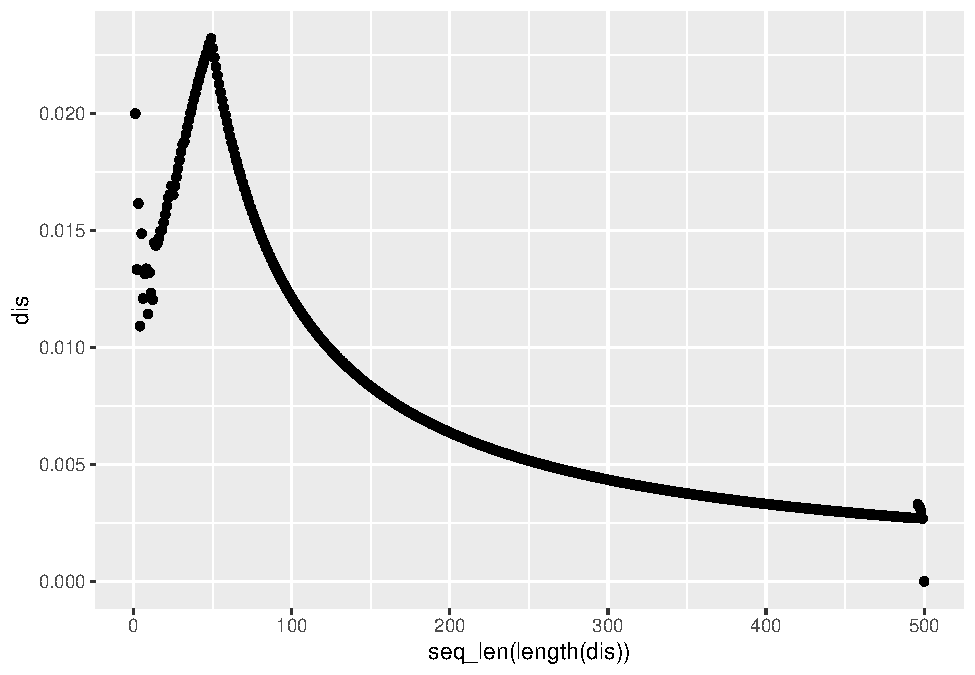
\includegraphics[width=0.95\linewidth]{figurasR/unnamed-chunk-33-1} \end{center}

En este caso se nos presenta la desproporción variando el número de
escaños posibles, en el presente caso se empieza por repartir un único
escaño hasta los 800 posibles escaños. La desproporción en el caso de un
escaño es muy alta como suele suceder en los métodos anteriormente
analizados, posteriormente cuanto mayor es el número de escaños a
repartir la desproporción va bajando constantemente.\\
En este método Imperiali podemos comprobar como el descenso de la
desproporción no es tan acusado como otros métodos anteriormente
analizados, empezando a tener una desproporción aceptable a partir de
los 500 escaños.\\
La diferencia de desproporción en los casos en los que hay pocos escaños
a repartir es alta, cuantos mas escaños a repartir la diferencia de
desproporción entre sucesivos escaños va reduciéndose y a números altos
de escaños a repartir la desproporción tiende a estabilizarse.

\hypertarget{imperiali-variando-el-nuxfamero-de-partidos}{%
\subsection{Imperiali variando el número de
partidos}\label{imperiali-variando-el-nuxfamero-de-partidos}}

\begin{center}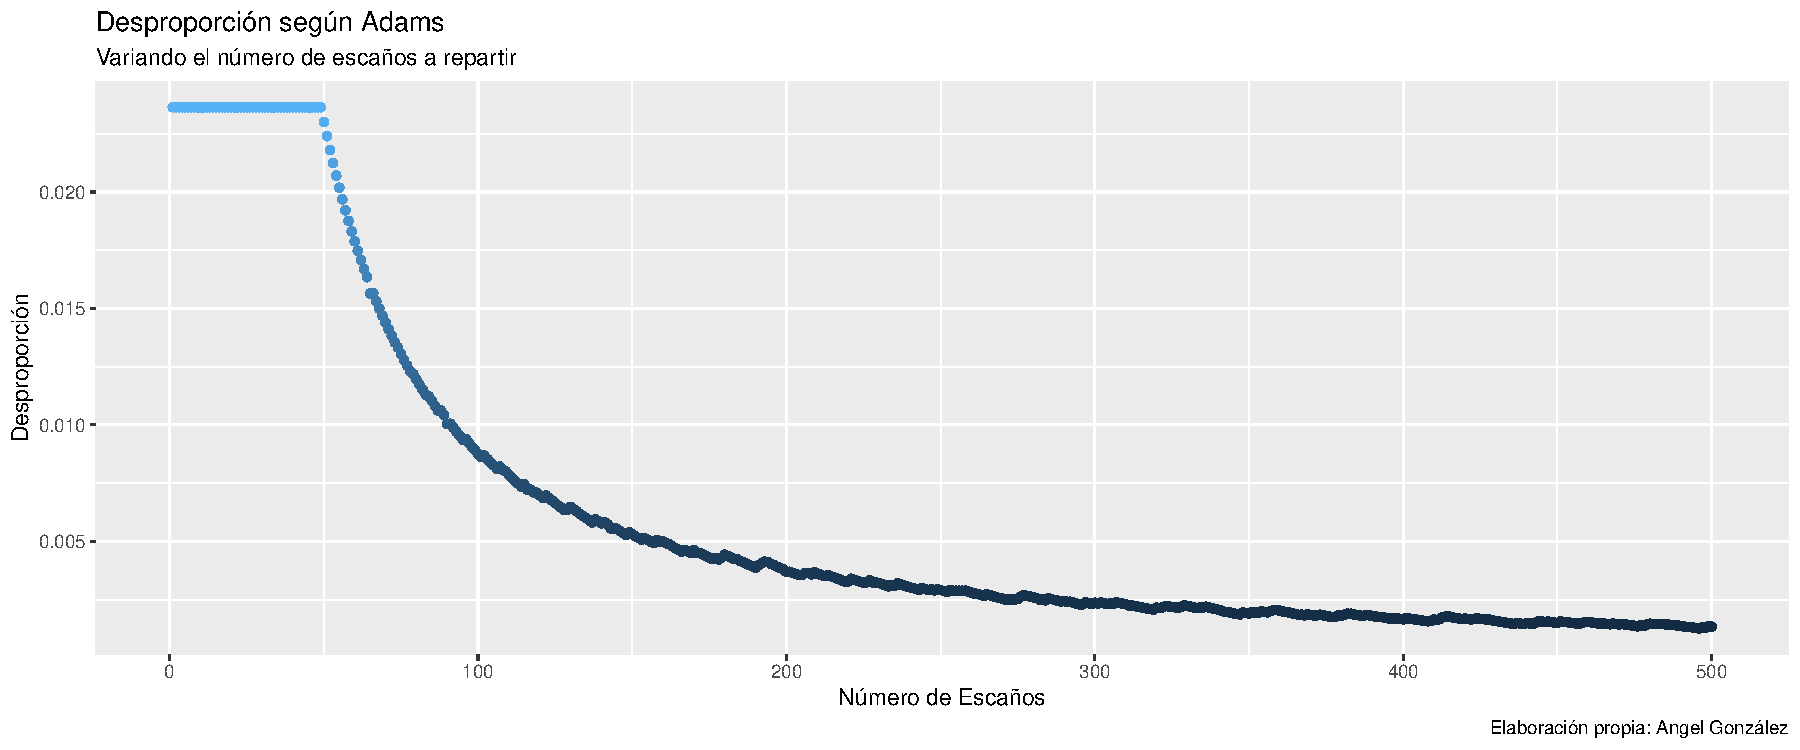
\includegraphics[width=0.95\linewidth]{figurasR/unnamed-chunk-34-1} \end{center}

En este caso únicamente modificamos el número de partidos presentes en
la elección, desde un único partido hasta 100 partidos que se presentan
a una elección ficticia. Observamos que cuando se presentan 2 o 3
partidos a las elecciones la desproporción es baja, va aumentando a
medida que se presentan más partidos, alcanzando el máximo de
desproporción con 24 partidos que se presentan a las elecciones, a
partir de ese punto la curva decrece constantemente. Entonces, según el
modelo Imperiali tendremos una mejor desproporción según se vaya
aumentando el número de partidos o bien si se presentan un número muy
reducido de partidos.

\hypertarget{imperiali-variando-la-concentraciuxf3n-del-voto}{%
\subsection{Imperiali variando la concentración del
voto}\label{imperiali-variando-la-concentraciuxf3n-del-voto}}

\begin{center}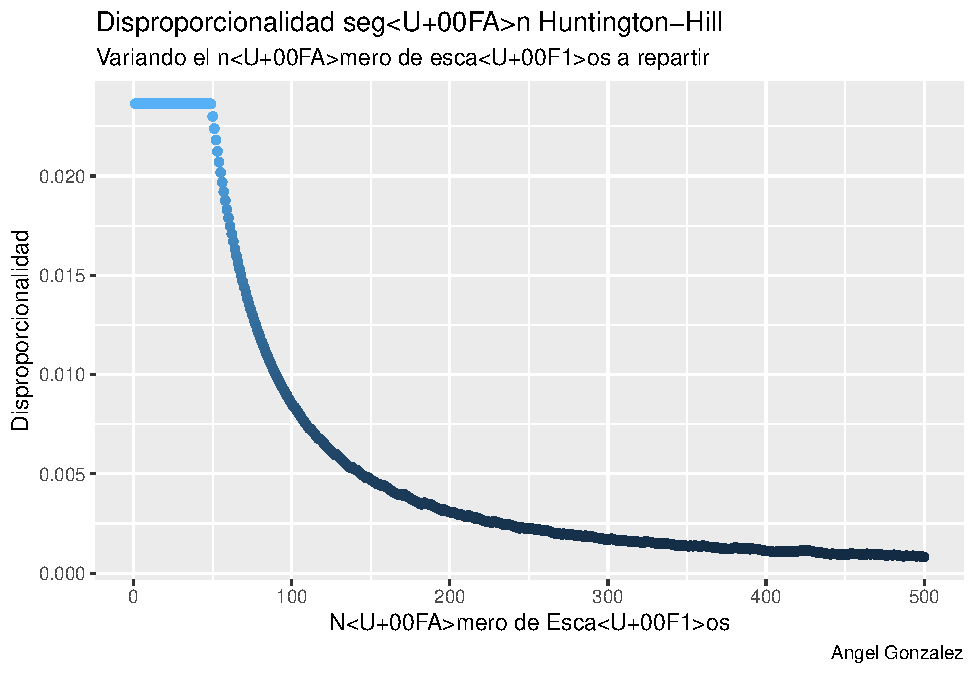
\includegraphics[width=0.95\linewidth]{figurasR/unnamed-chunk-35-1} \end{center}

En el presente gráfico variamos la concentración del voto en unas
elecciones ficticias, comenzamos con una concentración de votos baja, es
decir, la diferencia de votos entre partidos es baja, hasta acabar con
una concentración de votos alta, en donde la diferencia de votos entre
partidos es muy grande. Observando el gráfico observamos que cuando la
concentración del voto es muy baja la desproporción está en un nivel
bajo, cuanto más concentración de voto podemos comprobar como la
desproporción aumenta hasta que alcanza un punto en donde alcanza el
máximo de desproporción, alrededor de una concentración del voto media y
a partir de ese punto la desproporción va bajando constantemente. El
reparto de escaños según la ley Imperiali obtiene su menor desproporción
en los escenarios en donde la diferencia de votos entre los partidos sea
muy baja, aunque en comparación con los métodos anteriormente analizados
su desproporción es significativamente mas alta.

\hypertarget{huntington-hill}{%
\section{Huntington-Hill}\label{huntington-hill}}

\hypertarget{huntington-hill-variando-el-nuxfamero-de-escauxf1os}{%
\subsection{Huntington-Hill variando el número de
escaños}\label{huntington-hill-variando-el-nuxfamero-de-escauxf1os}}

\begin{center}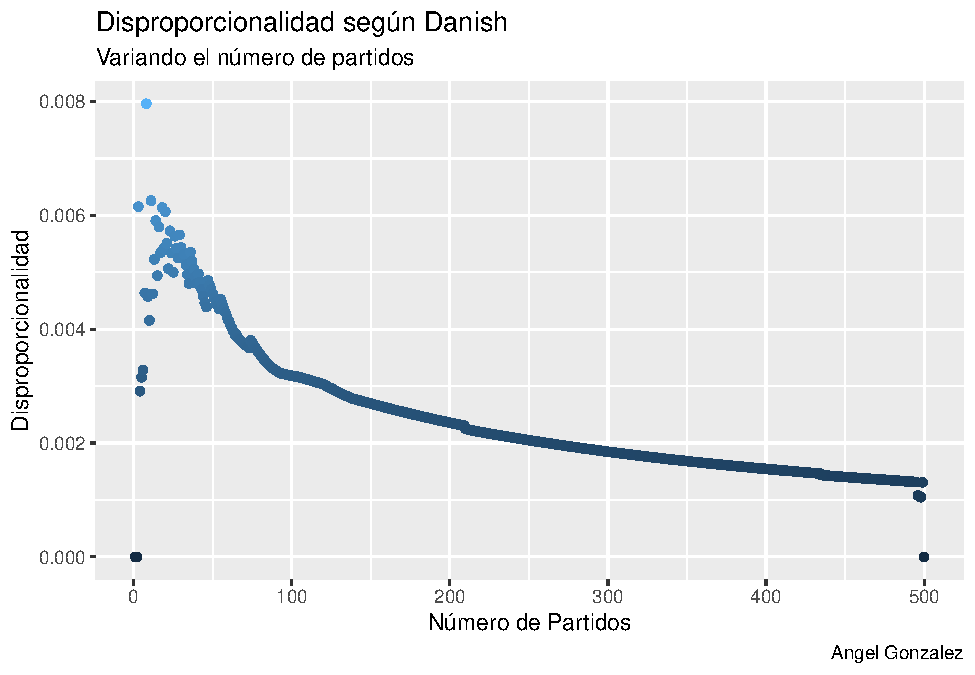
\includegraphics[width=0.95\linewidth]{figurasR/unnamed-chunk-38-1} \end{center}

En este caso se nos presenta la desproporción variando el número de
escaños posibles, se empieza por repartir un único escaño hasta los 800
posibles escaños. Observamos que la desproporción en el caso de repartir
unos pocos escaños es muy alta, desciende rápidamente en los primeros
escaños hasta llegar alrededor de los 10 a 20 escaños, en donde se
estabiliza temporalmente, a partir de los 20 escaños vuelve a descender
rápidamente. Este comportamiento se entiende por el hecho de repartir
más escaños que partidos se presentan a las elecciones. A partir de los
50 escaños desciende lentamente y tiende a estabilizarse cuanto mayor
número de escaños se reparten. Sería deseable elegir un número de
escaños entre los 100 y 200, en donde ya parece que se estabiliza y
presenta niveles muy bajos de desproporción.

\hypertarget{huntington-hill-variando-el-nuxfamero-de-partidos}{%
\subsection{Huntington-Hill variando el número de
partidos}\label{huntington-hill-variando-el-nuxfamero-de-partidos}}

\begin{center}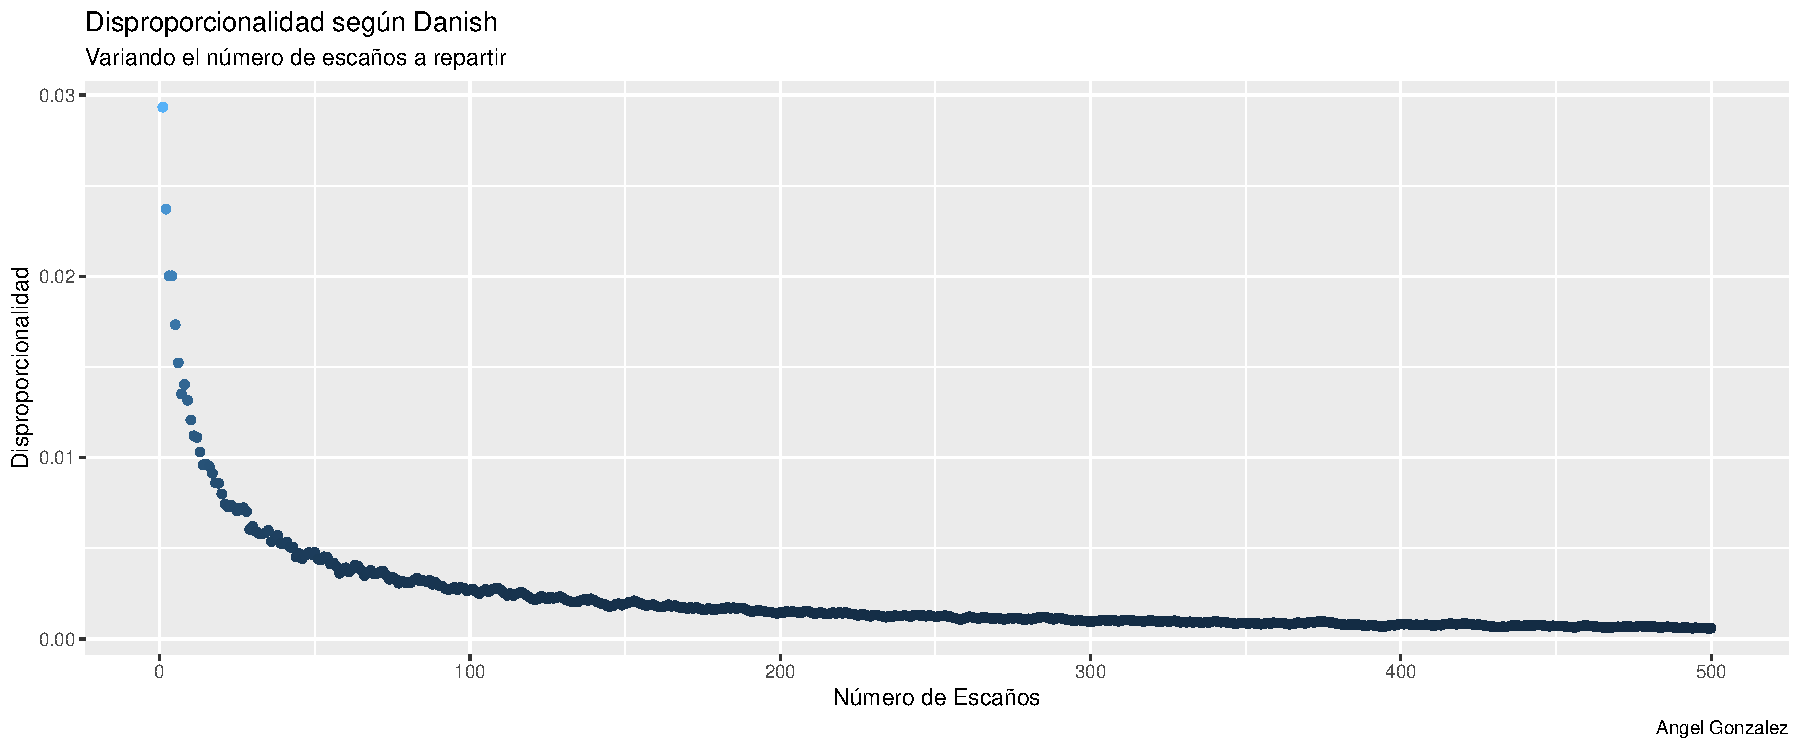
\includegraphics[width=0.95\linewidth]{figurasR/unnamed-chunk-39-1} \end{center}

En este caso únicamente modificamos el número de partidos presentes en
la elección, desde un único partido hasta 100 partidos que se presentan
a una elección ficticia.\\
Observamos que cuando se presentan de 2 a 24 partidos a las elecciones
la desproporción es bastante baja, va aumentando significativamente a
medida que se presentan más partidos, alcanzando el máximo de
desproporción con 50 partidos que se presentan a las elecciones, a
partir de los 50 partidos la curva cambia drásticamente, baja la
desproporción y comienza a decrecer. Esto es debido a que se reparten
menos escaños que partidos se presentan a las elecciones. Lo particular
de este método respecto a otros métodos es que la menor desproporción se
obtiene en el caso de que se presenten a las elecciones pocos partidos o
muchos partidos y que en los 50 partidos alcanza el máximo de
desproporción.

\hypertarget{huntington-hill-variando-la-concentraciuxf3n-del-voto}{%
\subsection{Huntington-Hill variando la concentración del
voto}\label{huntington-hill-variando-la-concentraciuxf3n-del-voto}}

\begin{center}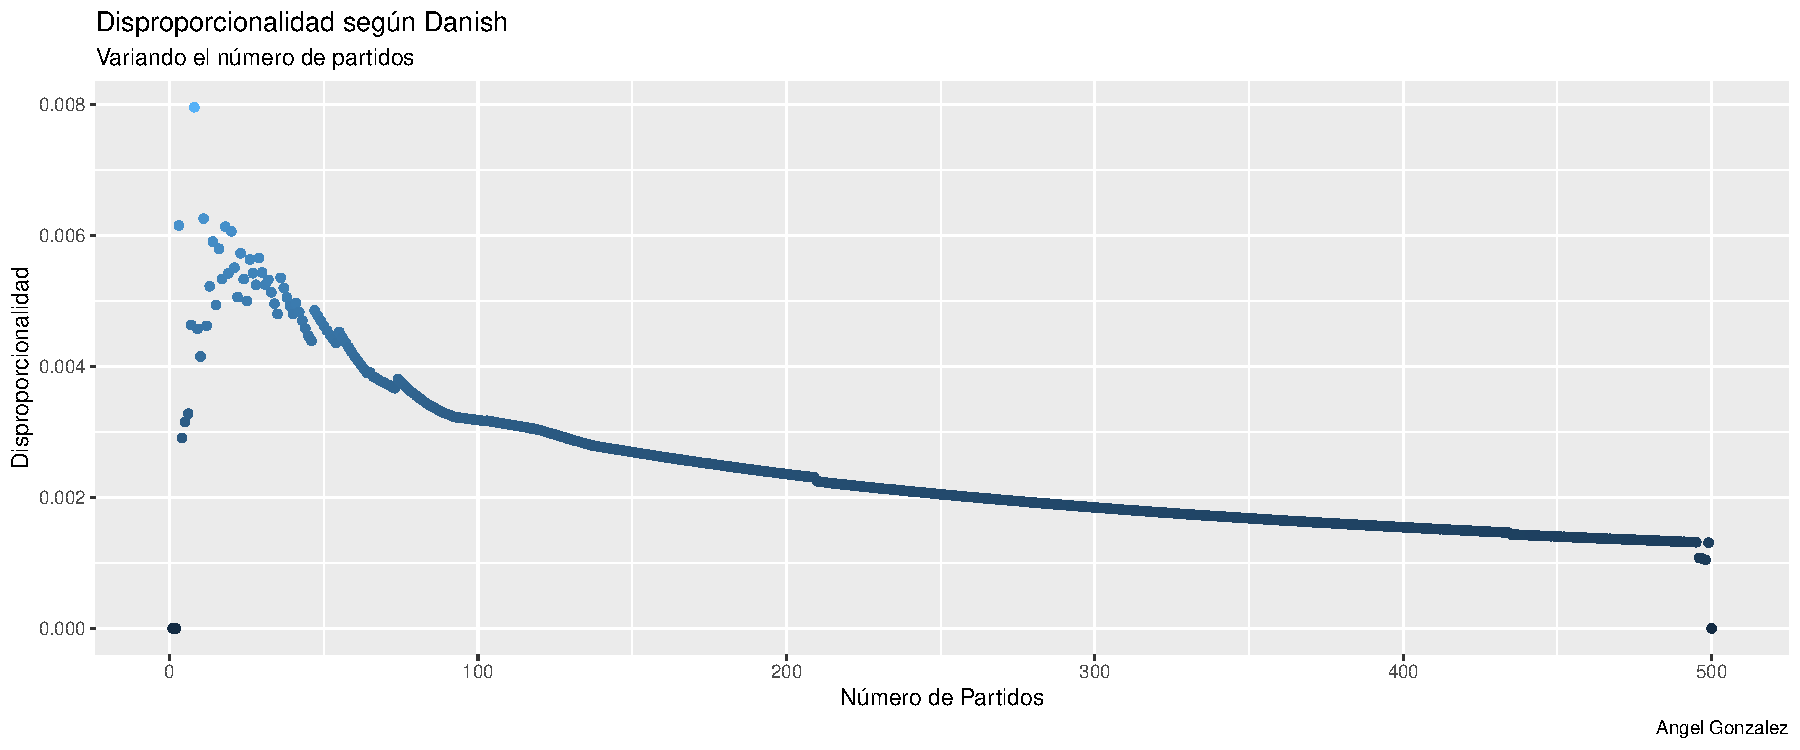
\includegraphics[width=0.95\linewidth]{figurasR/unnamed-chunk-40-1} \end{center}

En el presente gráfico variamos la concentración del voto en unas
elecciones ficticias, comenzamos con una concentración de votos baja, es
decir, la diferencia de votos entre partidos es baja, hasta acabar con
una concentración de votos alta, en donde la diferencia de votos entre
partidos es muy grande.\\
En el gráfico observamos que cuando la concentración del voto es muy
baja la desproporción está en un nivel bajo, desproporción que se
mantiene baja cuando la concentración de los votos es media, y que a
partir de una concentración de votos media-alta la desproporción va
aumentando cuanto más diferencia de votos entre partidos se presenten.\\
Así podemos concluir que el reparto de escaños según la ley
Huntington-Hill es mejor cuanto menor concentración de voto tengan los
partidos entre ellos o cuando la concentración de voto sea media,
presenta un comportamiento diferente respecto a los otros métodos en
donde cuanto mayor concentración de votos, menor desproporción. No es un
buen método para el caso en que los votos estén concentrados en pocos
partidos.

\hypertarget{adams}{%
\section{Adams}\label{adams}}

\hypertarget{adams-variando-el-nuxfamero-de-escauxf1os}{%
\subsection{Adams variando el número de
escaños}\label{adams-variando-el-nuxfamero-de-escauxf1os}}

\begin{center}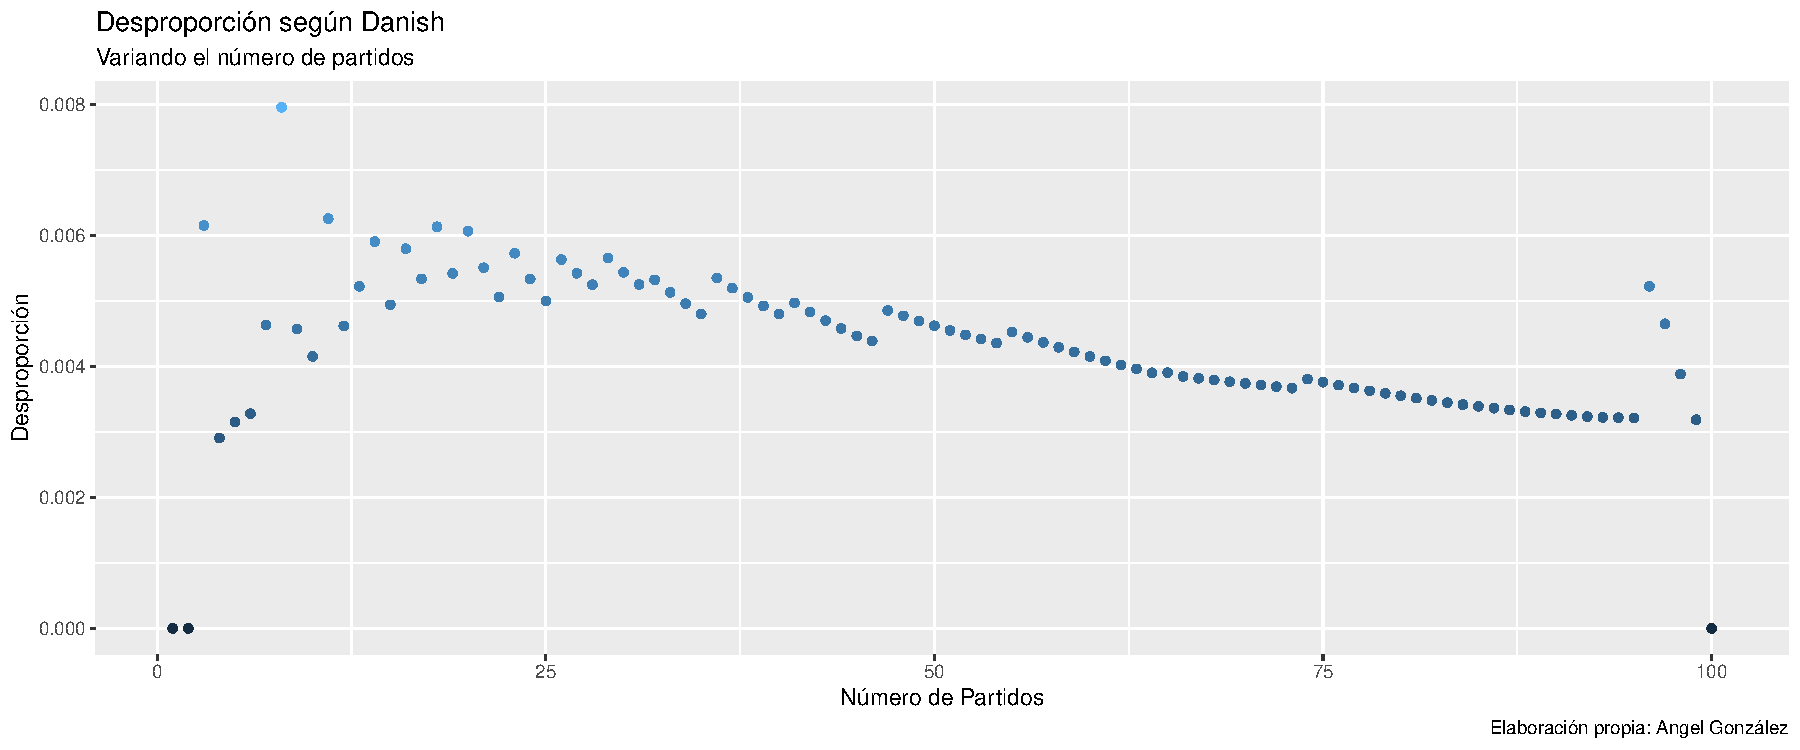
\includegraphics[width=0.95\linewidth]{figurasR/unnamed-chunk-43-1} \end{center}

En este caso se nos presenta la desproporción variando el número de
escaños posibles, se empieza por repartir un único escaño hasta los 800
posibles escaños. Observamos que la desproporción en el caso de un
escaño es muy alta, en este método también observamos una alta
desproporción inicial que se mantiene hasta los 50 escaños,
posteriormente cuanto mayor es el número de escaños a repartir la
desproporción va bajando. Sucede en este caso la misma situación que en
el método Huntington-Hill, en donde el comportamiento difiere si se
reparten más escaños que partidos se presentan a las elecciones. En
nuestro caso sucede en los 20 escaños a repartir porque hay 20 partidos
que se presentan a las elecciones. Este método presenta una
desproporción que se reduce algo más lentamente que otros métodos,
comenzando a ser aceptable a partir de los 100 escaños aproximadamente.

\hypertarget{adams-variando-el-nuxfamero-de-partidos}{%
\subsection{Adams variando el número de
partidos}\label{adams-variando-el-nuxfamero-de-partidos}}

\begin{center}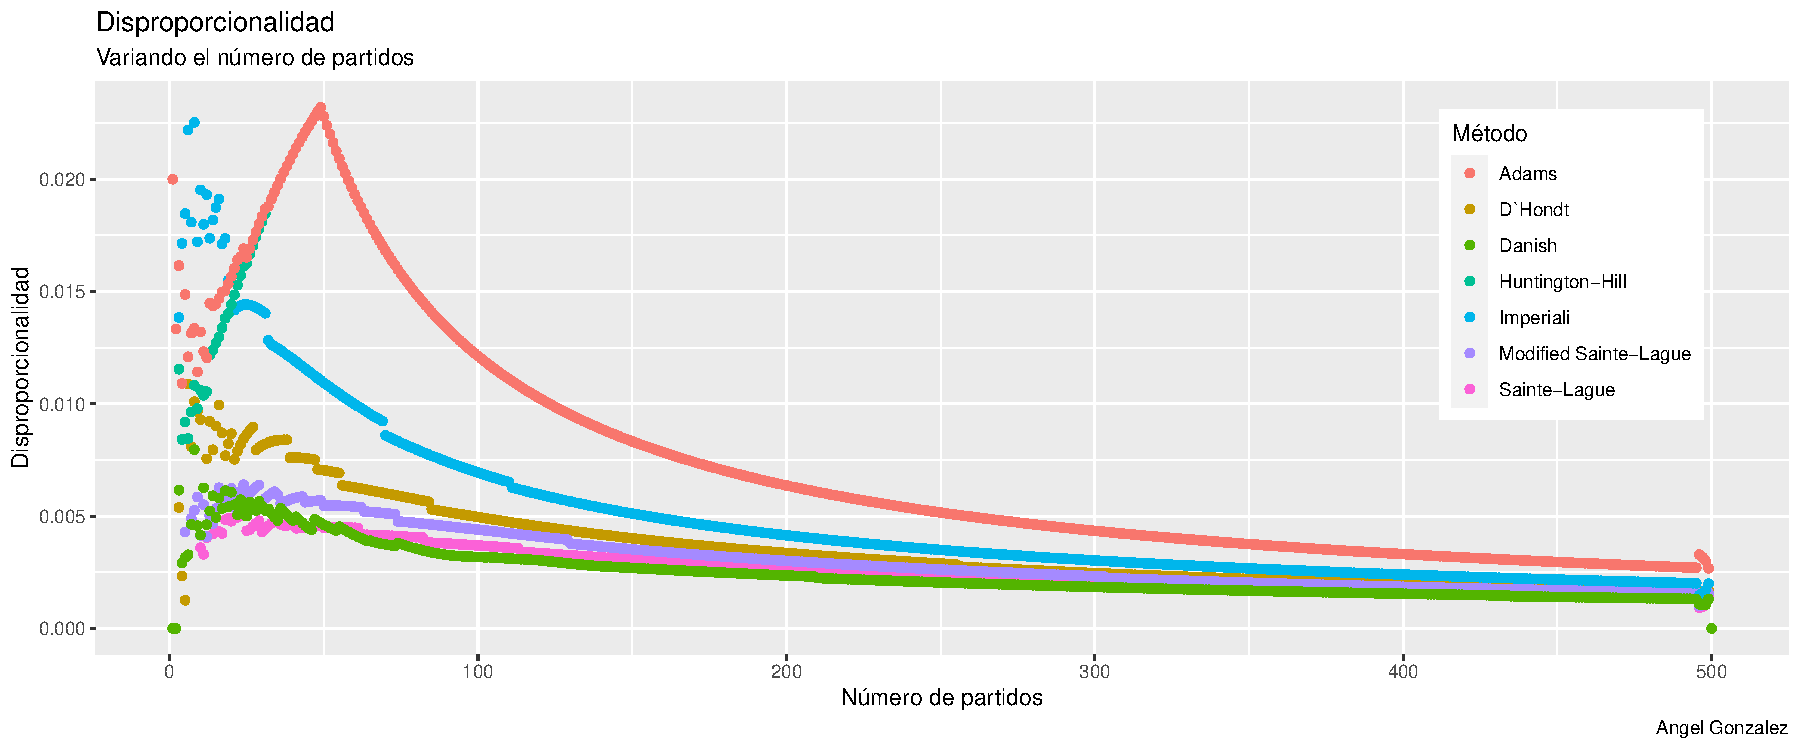
\includegraphics[width=0.95\linewidth]{figurasR/unnamed-chunk-44-1} \end{center}

En este caso únicamente modificamos el número de partidos presentes en
la elección, desde un único partido hasta 100 partidos que se presentan
a una elección ficticia.\\
Observamos que cuando se presentan de 2 a 23 partidos a las elecciones
la desproporción es baja con una variabilidad alta, como sucedía con el
método Huntington-Hill, va aumentando a medida que se presentan más
partidos, alcanzando el máximo de desproporción con 50 partidos que se
presentan a las elecciones, a partir de los 50 partidos que se presentan
a las elecciones sucede que se empiezan a repartir menos escaños que
partidos se presentan a las elecciones, debido a ello baja la
desproporción y la curva comienza a decrecer.\\
En este método Adams obtenemos el mejor resultado cuanto menor número de
partidos se presenten a las elecciones o bien cuando se presenten muchos
partidos, no siendo aconsejable utilizar este método cuando se presenten
entre 25 a 50 partidos a las elecciones.

\hypertarget{adams-variando-la-concentraciuxf3n-del-voto}{%
\subsection{Adams variando la concentración del
voto}\label{adams-variando-la-concentraciuxf3n-del-voto}}

\begin{center}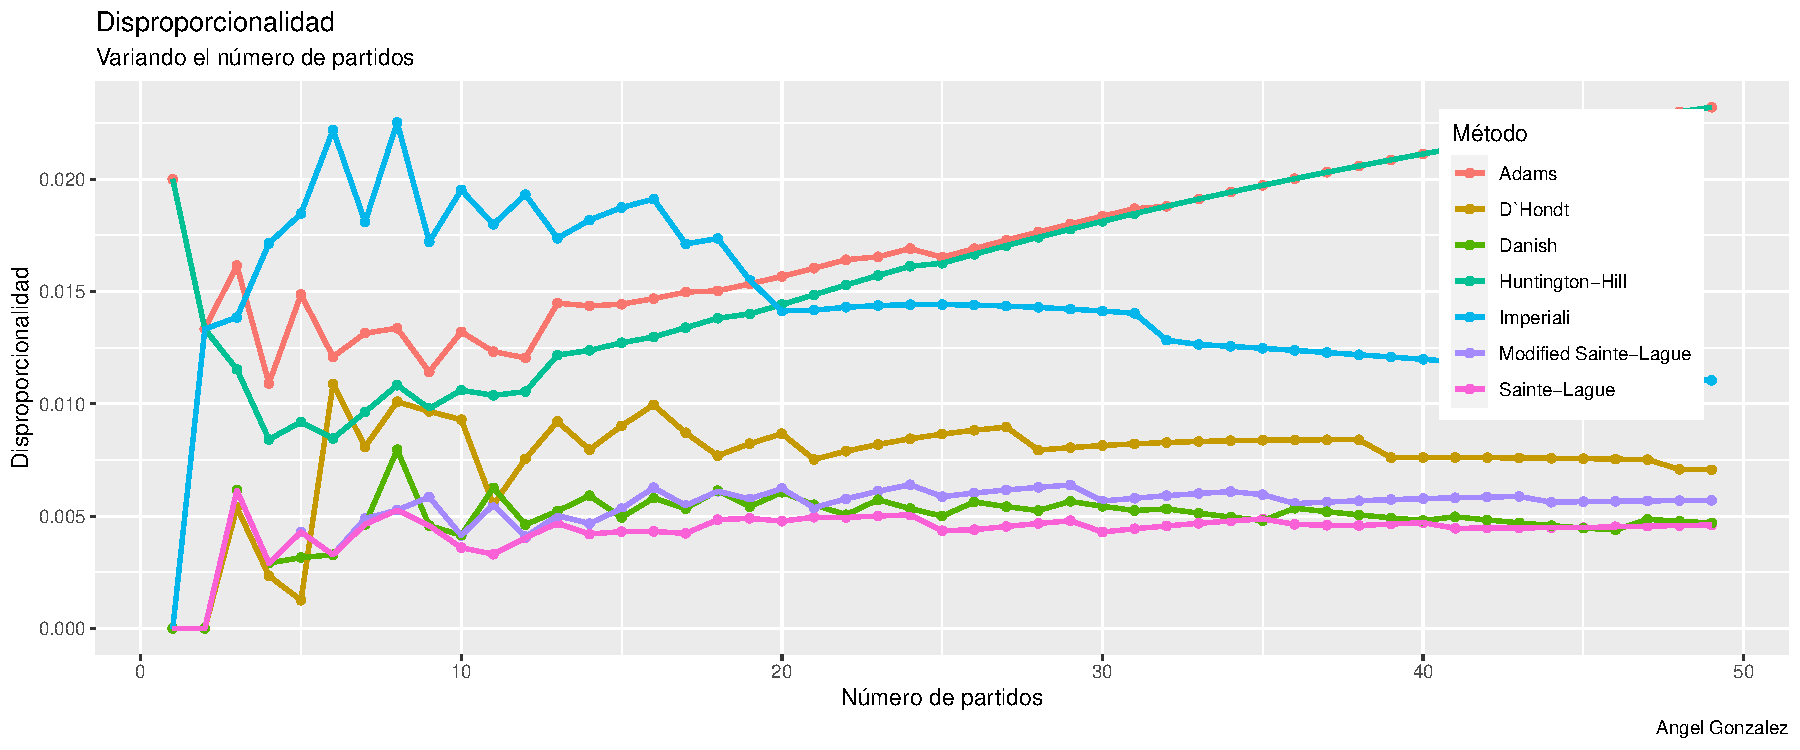
\includegraphics[width=0.95\linewidth]{figurasR/unnamed-chunk-45-1} \end{center}

En el presente gráfico variamos la concentración del voto en unas
elecciones ficticias, comenzamos con una concentración de votos baja, es
decir, la diferencia de votos entre partidos es baja, hasta acabar con
una concentración de votos alta, en donde la diferencia de votos entre
partidos es muy grande.\\
Según el gráfico observamos que cuando la concentración del voto es muy
baja, la desproporción también está en un nivel bajo. Cuanto más
concentración de voto se encuentren entre los partidos la desproporción
va aumentando cada vez más, éste es un método que depende mucho de la
concentración del voto.\\
Podemos concluir que el reparto de escaños según la ley Adams es mejor
cuanto menor concentración de voto tengan los partidos entre ellos, y
será peor cuanto mayor concentración de voto se presente.

\hypertarget{danish}{%
\section{Danish}\label{danish}}

\hypertarget{danish-variando-el-nuxfamero-de-escauxf1os}{%
\subsection{Danish variando el número de
escaños}\label{danish-variando-el-nuxfamero-de-escauxf1os}}

\begin{center}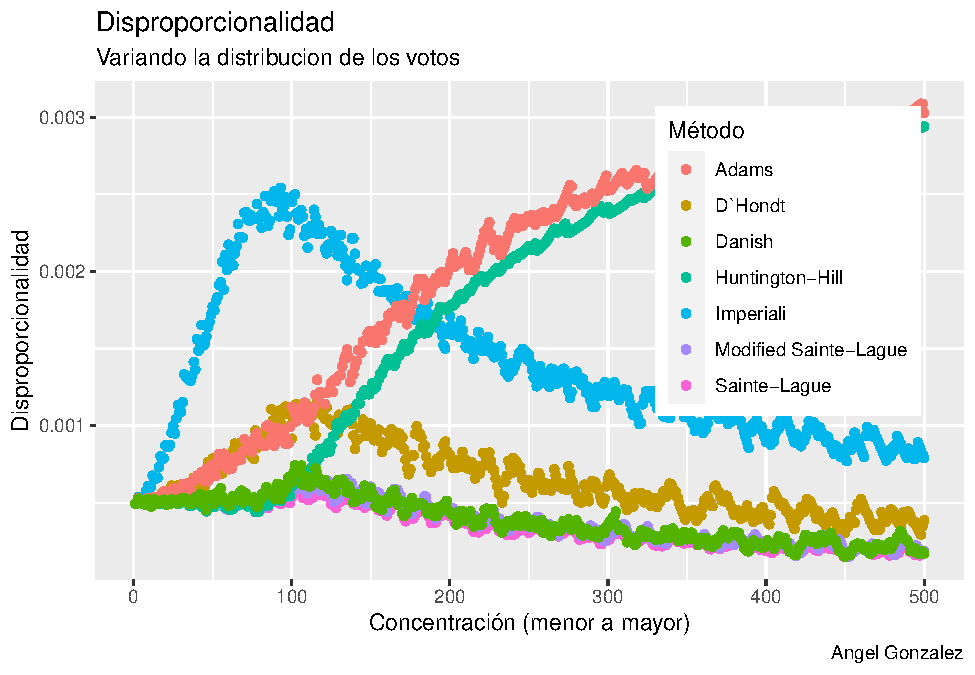
\includegraphics[width=0.95\linewidth]{figurasR/unnamed-chunk-48-1} \end{center}

En este caso se nos presenta la desproporción variando el número de
escaños posibles, en el presente caso se empieza por repartir un único
escaño hasta los 800 posibles escaños. Observamos que la desproporción
en el caso de un escaño es muy alta, posteriormente cuanto mayor es el
número de escaños a repartir la desproporción va bajando. La diferencia
de desproporción en los casos en los que hay pocos escaños a repartir es
alta, cuantos mas escaños a repartir la diferencia de desproporción
entre sucesivos escaños va reduciéndose, a números altos de escaños a
repartir la desproporción tiende a estabilizarse.

\hypertarget{danish-variando-el-nuxfamero-de-partidos}{%
\subsection{Danish variando el número de
partidos}\label{danish-variando-el-nuxfamero-de-partidos}}

\begin{center}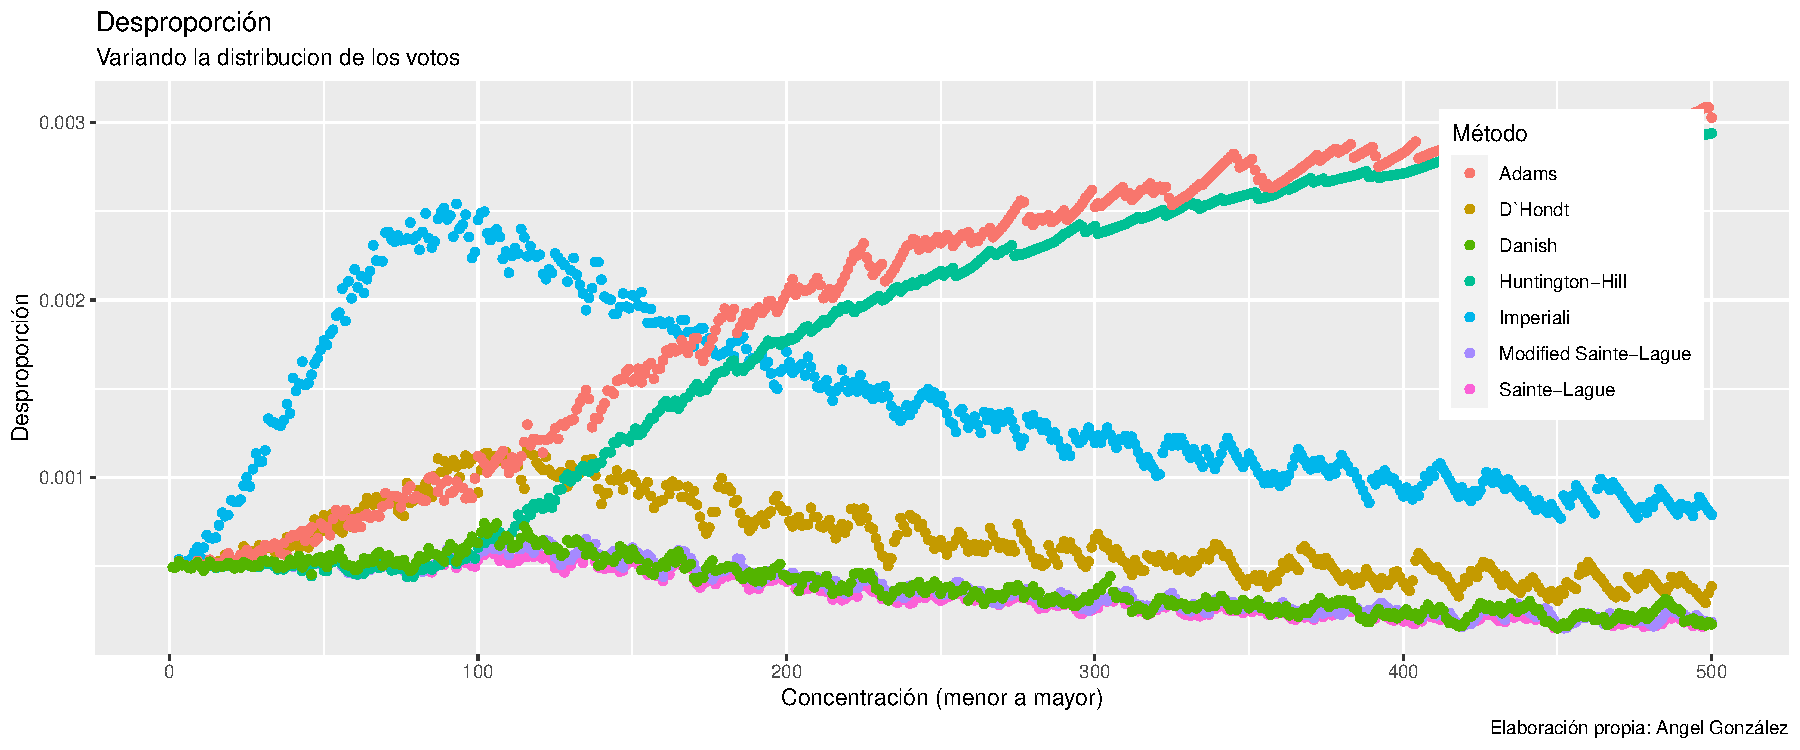
\includegraphics[width=0.95\linewidth]{figurasR/unnamed-chunk-49-1} \end{center}

En este caso únicamente modificamos el número de partidos presentes en
la elección, desde un único partido hasta 100 partidos que se presentan
a una elección ficticia.\\
Observamos que cuando se presentan de 2 a 25 partidos a las elecciones
la desproporción es media-alta, alcanza su máximo con 25 partidos, a
partir del cual comienza a decrecer. Podemos apreciar en el gráfico que
para un número bajo de partidos que se presentan a las elecciones la
desproporción es medio-alta y estable dentro de un mismo rango, cuanto
mayor número de partidos se presentan en las elecciones menor es la
desproporción que encontramos. Según lo visto en el gráfico, en el
método Danish obtenemos el mejor resultado cuanto más partidos se
presenten a las elecciones.

\hypertarget{danish-variando-la-concentraciuxf3n-del-voto}{%
\subsection{Danish variando la concentración del
voto}\label{danish-variando-la-concentraciuxf3n-del-voto}}

\begin{center}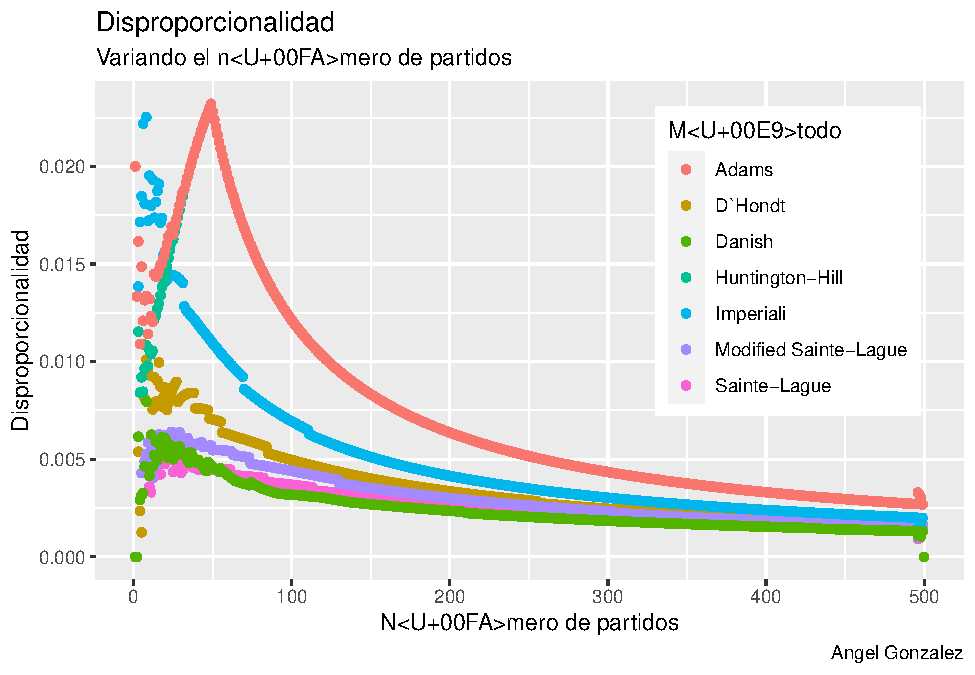
\includegraphics[width=0.95\linewidth]{figurasR/unnamed-chunk-50-1} \end{center}

En el presente gráfico variamos la concentración del voto en unas
elecciones ficticias, comenzamos con una concentración de votos baja, es
decir, la diferencia de votos entre partidos es baja, hasta acabar con
una concentración de votos alta, en donde la diferencia de votos entre
partidos es muy grande.\\
Observando el gráfico observamos que la concentración del voto no
depende de la desproporción, que se encuentra en un mismo rango sea la
concentración del voto alta o baja.\\
El reparto de escaños según la ley Danish presenta unas características
muy deseables, el nivel de desproporción es extremadamente bajo y no
depende significativamente de la concentración del voto.

\hypertarget{lr-hare}{%
\section{LR Hare}\label{lr-hare}}

\begin{Shaded}
\begin{Highlighting}[]
\NormalTok{Para diferenciar entre los métodos de resto mayor y promedio mayor, }
\NormalTok{procederemos a añadir el prefijo }\FunctionTok{LR}\NormalTok{ ( Largest Remainder ) }
\NormalTok{a los métodos de resto mayor.}
\end{Highlighting}
\end{Shaded}

\hypertarget{lr-hare-variando-el-nuxfamero-de-escauxf1os}{%
\subsection{LR Hare variando el número de
escaños}\label{lr-hare-variando-el-nuxfamero-de-escauxf1os}}

\begin{center}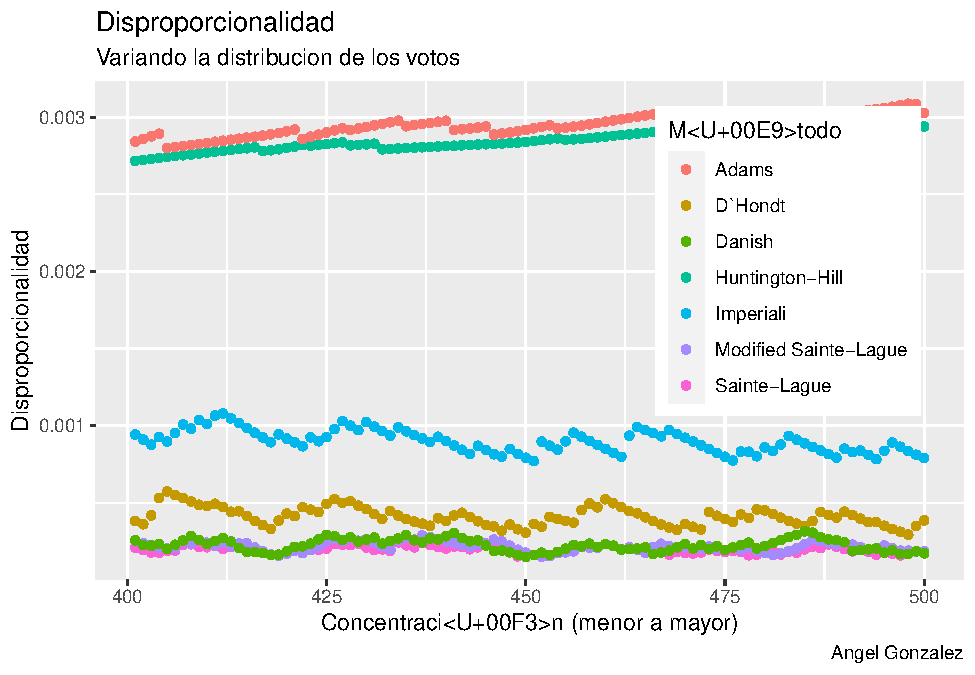
\includegraphics[width=0.95\linewidth]{figurasR/unnamed-chunk-53-1} \end{center}

En este caso se nos presenta la desproporción variando el número de
escaños posibles, en el presente caso se empieza por repartir un único
escaño hasta los 800 posibles escaños. Observamos que la desproporción
en el caso de un escaño es muy alta, posteriormente cuanto mayor es el
número de escaños a repartir la desproporción desciende rápidamente en
comparación con métodos anteriormente analizados, llegando a un nivel
aceptable de desproporción entre los 100 a 200 escaños.

\hypertarget{lr-hare-variando-el-nuxfamero-de-partidos}{%
\subsection{LR Hare variando el número de
partidos}\label{lr-hare-variando-el-nuxfamero-de-partidos}}

\begin{center}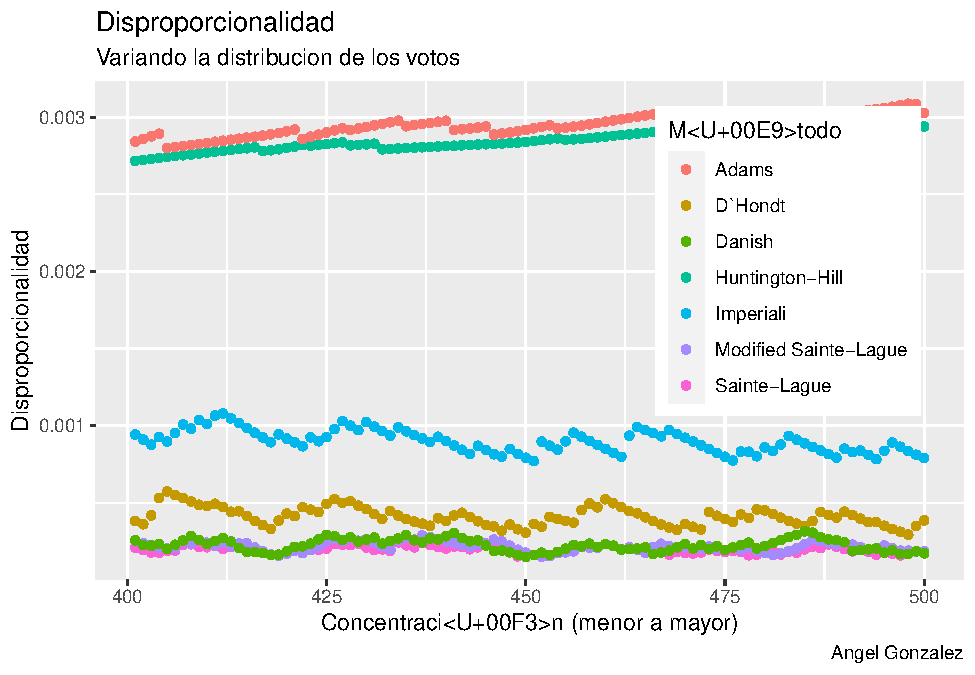
\includegraphics[width=0.95\linewidth]{figurasR/unnamed-chunk-54-1} \end{center}

En este caso únicamente modificamos el número de partidos presentes en
la elección, desde un único partido hasta 100 partidos que se presentan
a una elección ficticia. Observamos que cuando se presentan un número
bajo de partidos a las elecciones, entre 2 a 25, la desproporción es
alta, va disminuyendo a medida que se presentan más partidos, alcanzando
el mínimo de desproporción cuantos más partidos se presenten a las
elecciones . Podemos apreciar en el gráfico que para un número bajo de
partidos que se presentan a las elecciones ( de 2 a 25 ) la dispersión
es alta pero decreciente, a partir de los 25 escaños la variabilidad
tiende a estabilizarse cuanto mayor número de partidos se presenten en
las elecciones.\\
Según el método LR Hare obtendremos el mejor resultado en términos de
desproporción cuanto más partidos se presenten a las elecciones.

\hypertarget{lr-hare-variando-la-concentraciuxf3n-del-voto}{%
\subsection{LR Hare variando la concentración del
voto}\label{lr-hare-variando-la-concentraciuxf3n-del-voto}}

\begin{center}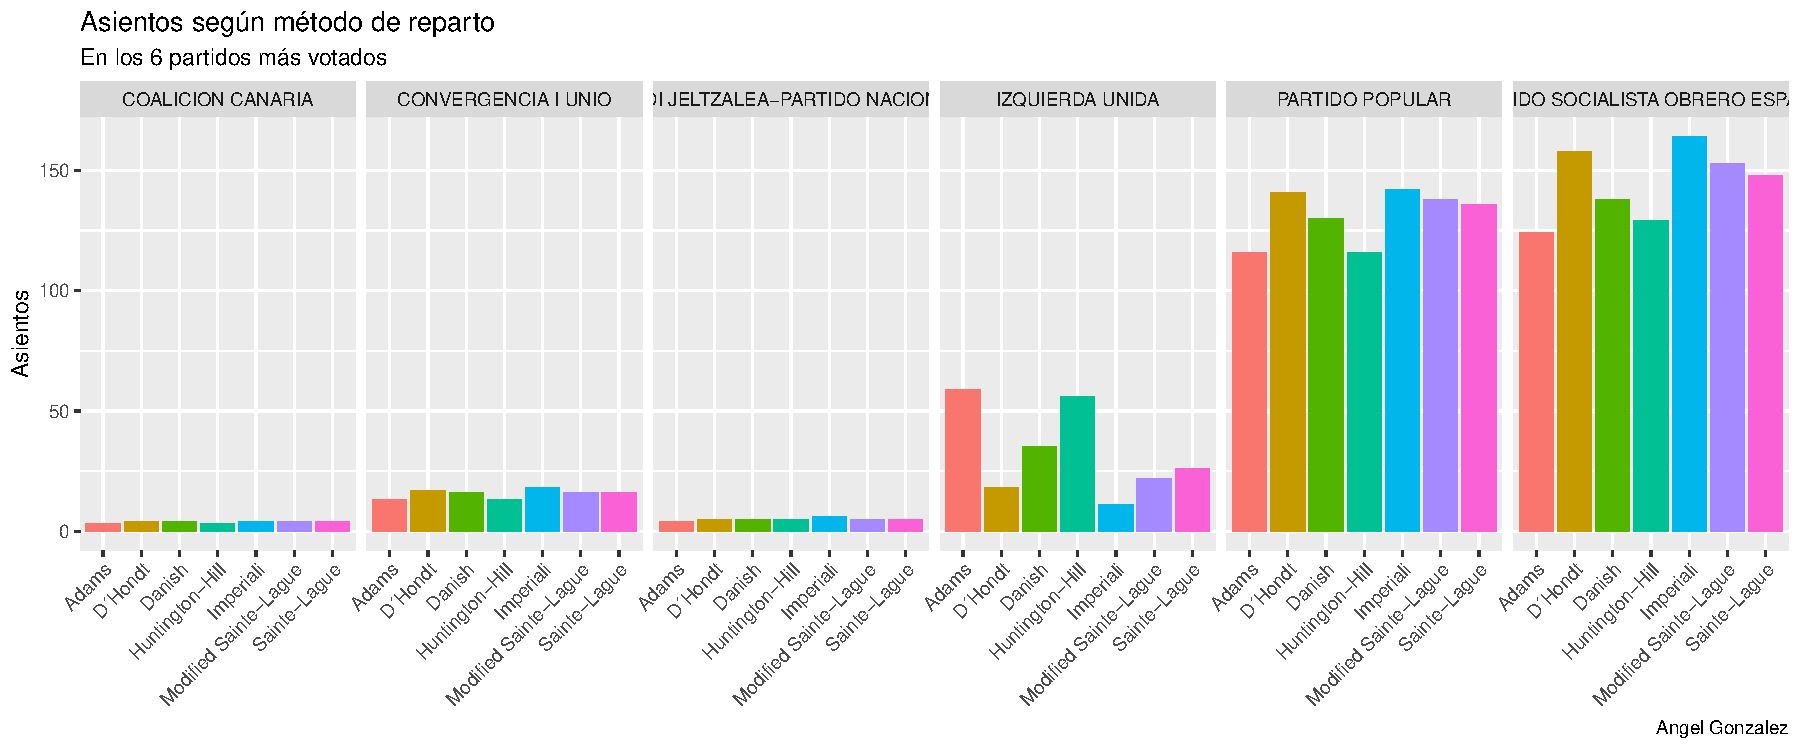
\includegraphics[width=0.95\linewidth]{figurasR/unnamed-chunk-55-1} \end{center}

En el presente gráfico variamos la concentración del voto en unas
elecciones ficticias, comenzamos con una concentración de votos baja, es
decir, la diferencia de votos entre partidos es baja, hasta acabar con
una concentración de votos alta, en donde la diferencia de votos entre
partidos es muy grande.\\
Observando el gráfico comprobamos como la concentración del voto no es
significativa para el nivel de desproporción, característica deseable.
Puede apreciarse una leve tendencia descendiente al aumentar la
concentración del voto, lo que podría dar a entender que a
concentraciones del voto extremadamente altas, el método LR-Hare
alcanzaría el mínimo nivel de desproporción.

\hypertarget{lr-droop}{%
\section{LR Droop}\label{lr-droop}}

\hypertarget{lr-droop-variando-el-nuxfamero-de-escauxf1os}{%
\subsection{LR Droop variando el número de
escaños}\label{lr-droop-variando-el-nuxfamero-de-escauxf1os}}

\begin{center}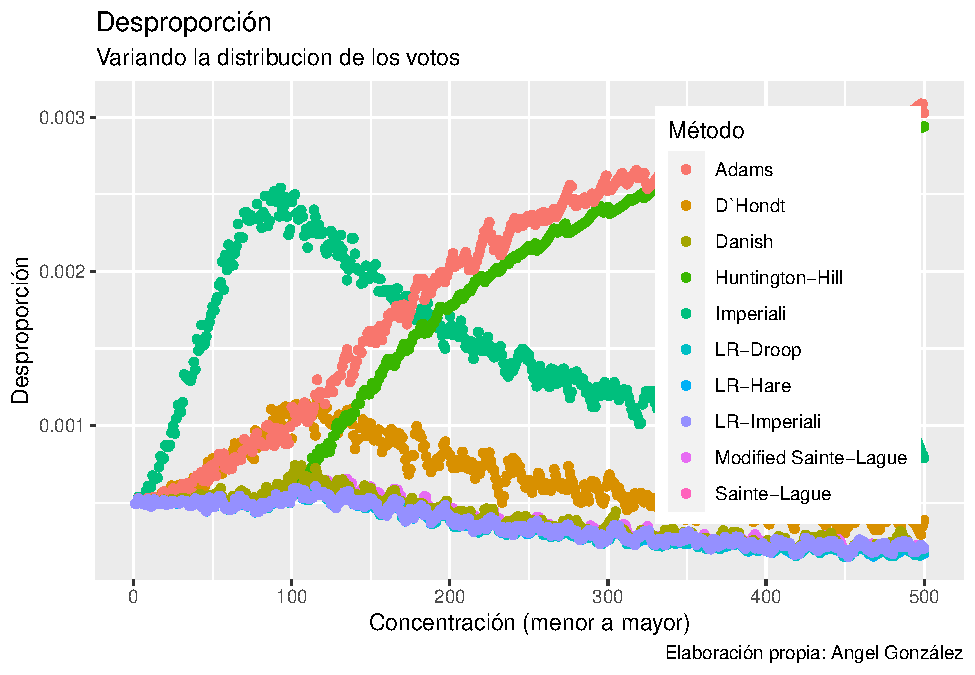
\includegraphics[width=0.95\linewidth]{figurasR/unnamed-chunk-58-1} \end{center}

En este caso se nos presenta la desproporción variando el número de
escaños posibles, en el presente caso se empieza por repartir un único
escaño hasta los 800 posibles escaños. La desproporción en el caso de
pocos escaños es muy alta, posteriormente cuanto mayor es el número de
escaños a repartir la desproporción va bajando constantemente.\\
La diferencia de desproporción entre los casos en los que hay pocos
escaños a repartir es alta, cuantos mas escaños a repartir la diferencia
de desproporción entre sucesivos escaños va reduciéndose, a números
altos de escaños a repartir la desproporción tiende a estabilizarse.\\
Este método LR-Droop alcanza niveles de desproporción aceptables a
partir de los 50 escaños y niveles deseables alrededor de los 200
escaños.

\hypertarget{lr-droop-variando-el-nuxfamero-de-partidos}{%
\subsection{LR Droop variando el número de
partidos}\label{lr-droop-variando-el-nuxfamero-de-partidos}}

\begin{center}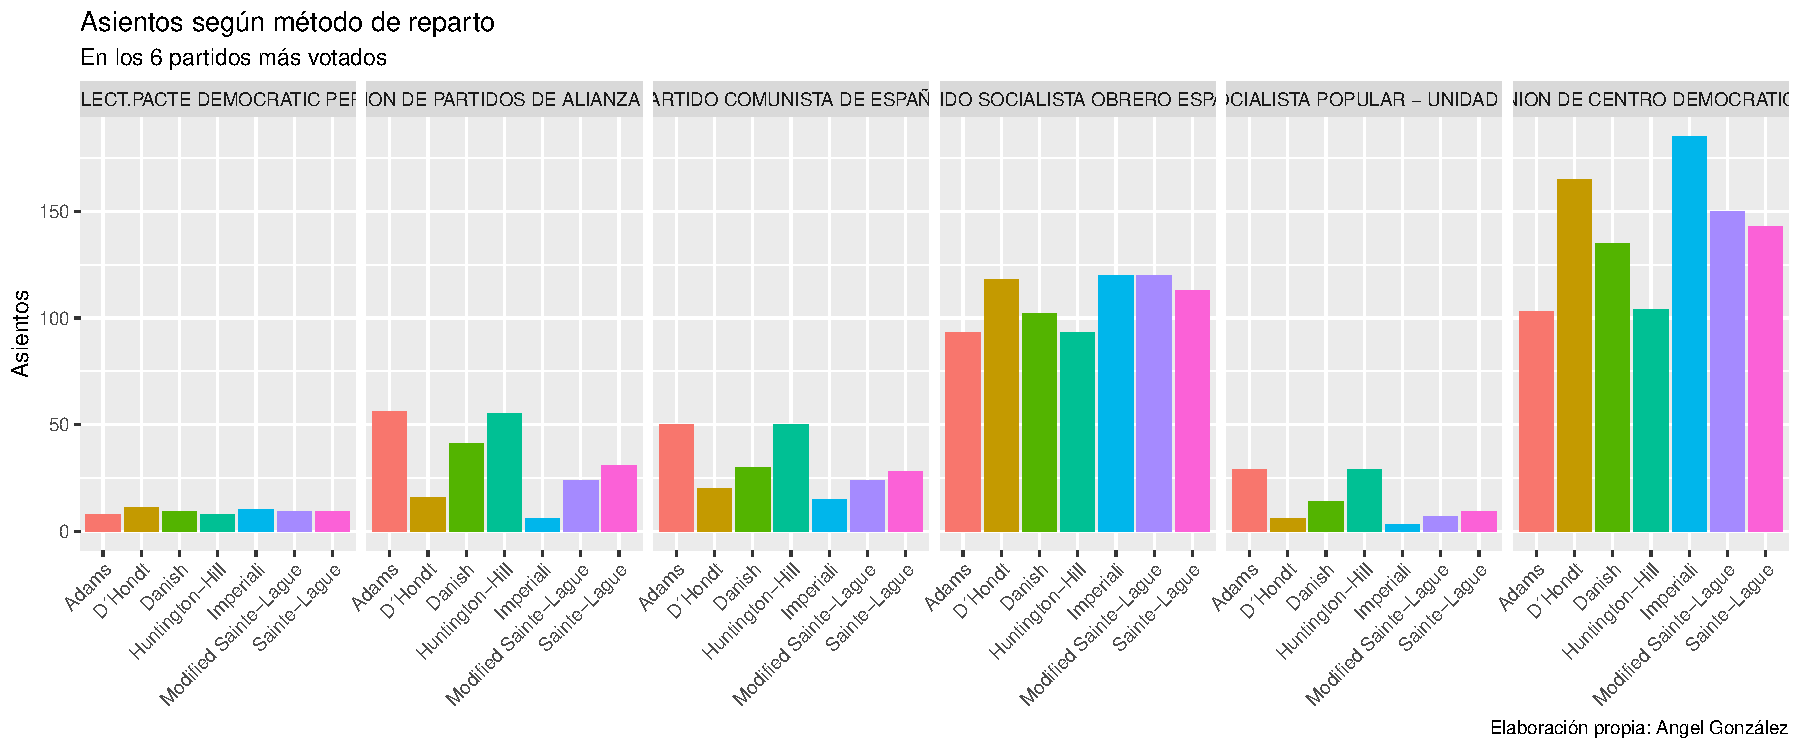
\includegraphics[width=0.95\linewidth]{figurasR/unnamed-chunk-59-1} \end{center}

En este caso únicamente modificamos el número de partidos presentes en
la elección, desde un único partido hasta 100 partidos que se presentan
a una elección ficticia. Gran variabilidad en el caso de que se
presenten un número bajo de partidos, hasta los 25 partidos, en esta
zona la desproporción es alta y se mueve en un mismo nivel. A partir de
los 25 partidos que se presentan a las elecciones la variabilidad cambia
totalmente respecto a la zona anterior y se vuelve estable, con un
descenso paulatino y no muy acusado. Se empieza a tener desproporciones
bajas a partir de los 50 partidos.\\
Según lo visto, en el método LR-Droop obtendremos el mejor resultado
cuanto más partidos se presenten a las elecciones.

\hypertarget{lr-droop-variando-la-concentraciuxf3n-del-voto}{%
\subsection{LR Droop variando la concentración del
voto}\label{lr-droop-variando-la-concentraciuxf3n-del-voto}}

\begin{center}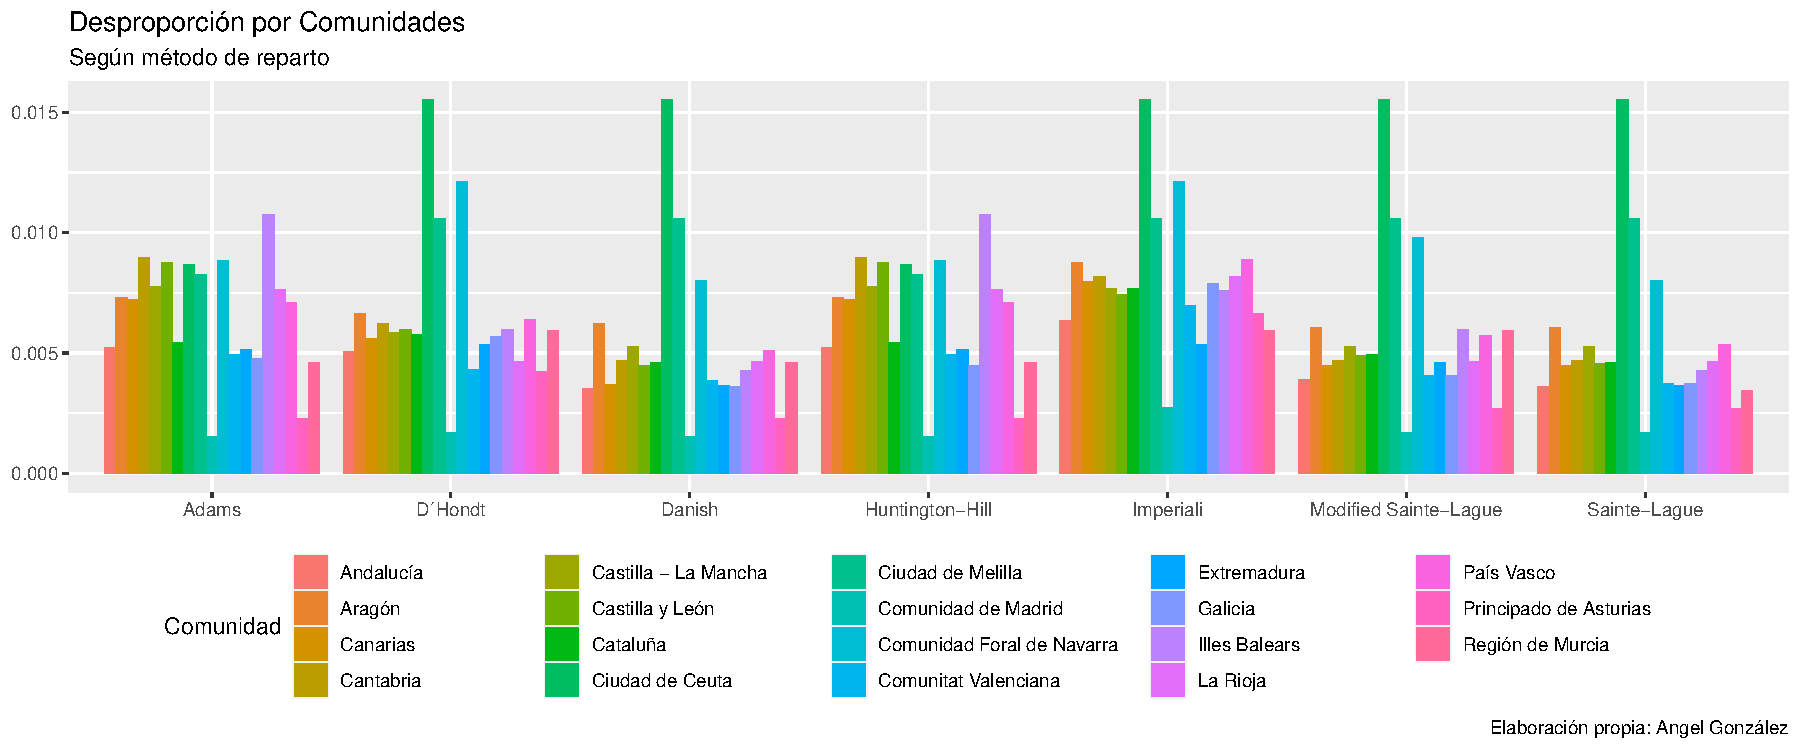
\includegraphics[width=0.95\linewidth]{figurasR/unnamed-chunk-60-1} \end{center}

En el presente gráfico variamos la concentración del voto en unas
elecciones ficticias, comenzamos con una concentración de votos baja, es
decir, la diferencia de votos entre partidos es baja, hasta acabar con
una concentración de votos alta, en donde la diferencia de votos entre
partidos es muy grande.\\
Observando el gráfico observamos que ya sea la concentración del voto
muy baja, media o muy alta,la desproporción se encuentra en un mismo
nivel, nivel en términos de desproporción muy bajos, cercanos al 0.
Dentro del rango entre que se encuentra la desproporción la variabilidad
es alta para cualquier nivel de concentración.\\
En este puede decirse que el método Droop posee una buena cualidad,
puesto que su proporcionalidad no depende de la concentración del voto.

\hypertarget{lr-imperiali}{%
\section{LR Imperiali}\label{lr-imperiali}}

\hypertarget{lr-imperiali-variando-el-nuxfamero-de-escauxf1os}{%
\subsection{LR Imperiali variando el número de
escaños}\label{lr-imperiali-variando-el-nuxfamero-de-escauxf1os}}

\begin{center}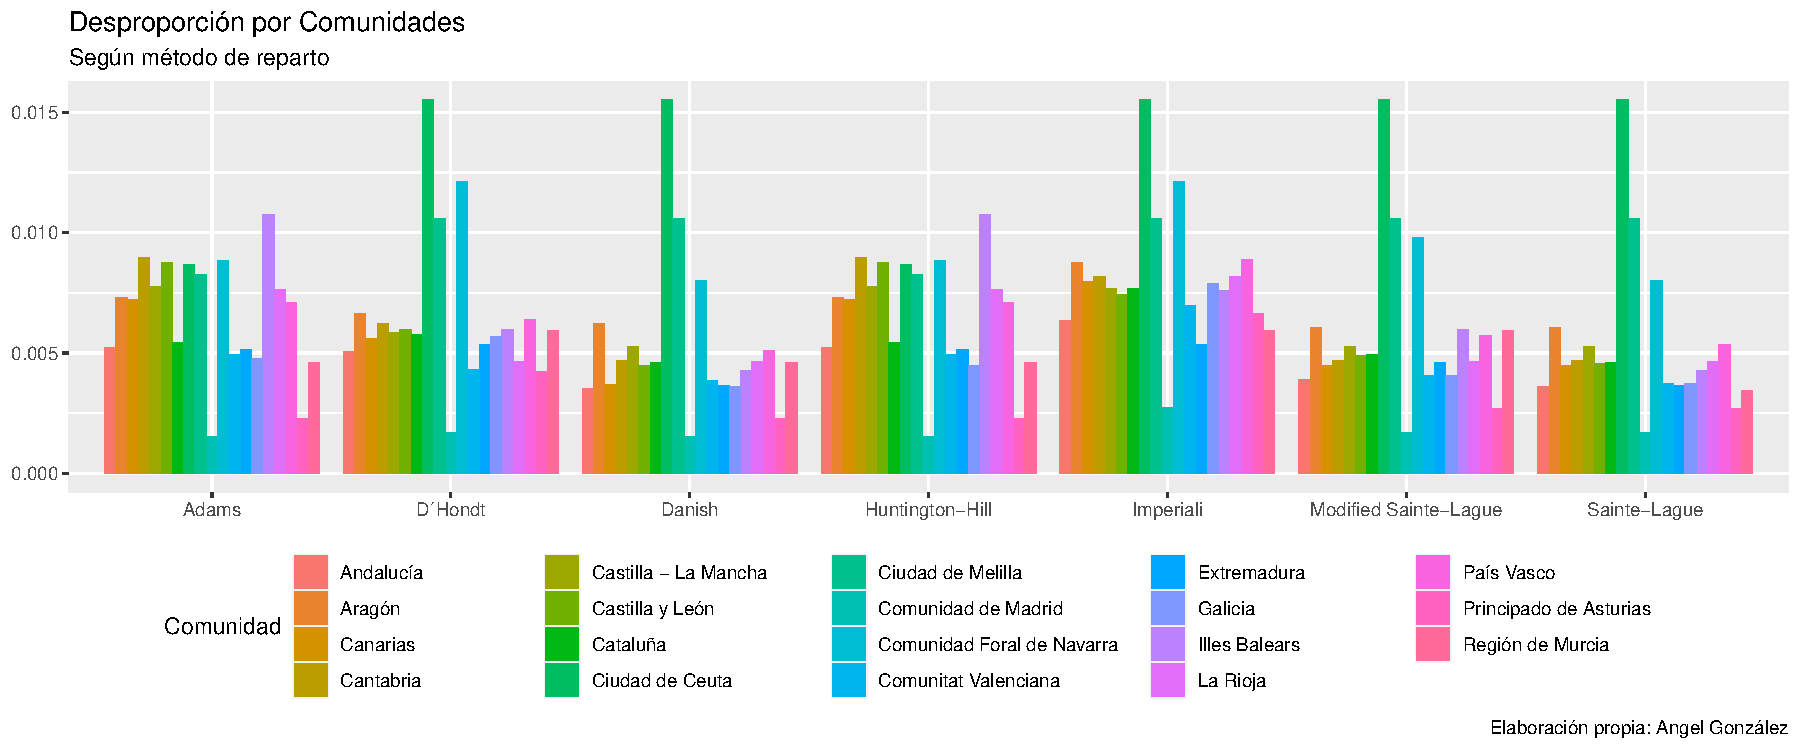
\includegraphics[width=0.95\linewidth]{figurasR/unnamed-chunk-63-1} \end{center}

En este caso se nos presenta la desproporción variando el número de
escaños posibles, en el presente caso se empieza por repartir un único
escaño hasta los 800 posibles escaños. No hay diferencia en el
comportamiento respecto a los otros métodos de restos mayores. La
desproporción en el caso que se repartan pocos escaños es muy alta,
posteriormente cuanto mayor es el número de escaños a repartir la
desproporción baja rápidamente hasta alcanzar niveles aceptables cuando
se reparten 100 escaños y niveles deseables a partir de los 200 escaños.

\hypertarget{lr-imperiali-variando-el-nuxfamero-de-partidos}{%
\subsection{LR Imperiali variando el número de
partidos}\label{lr-imperiali-variando-el-nuxfamero-de-partidos}}

\begin{center}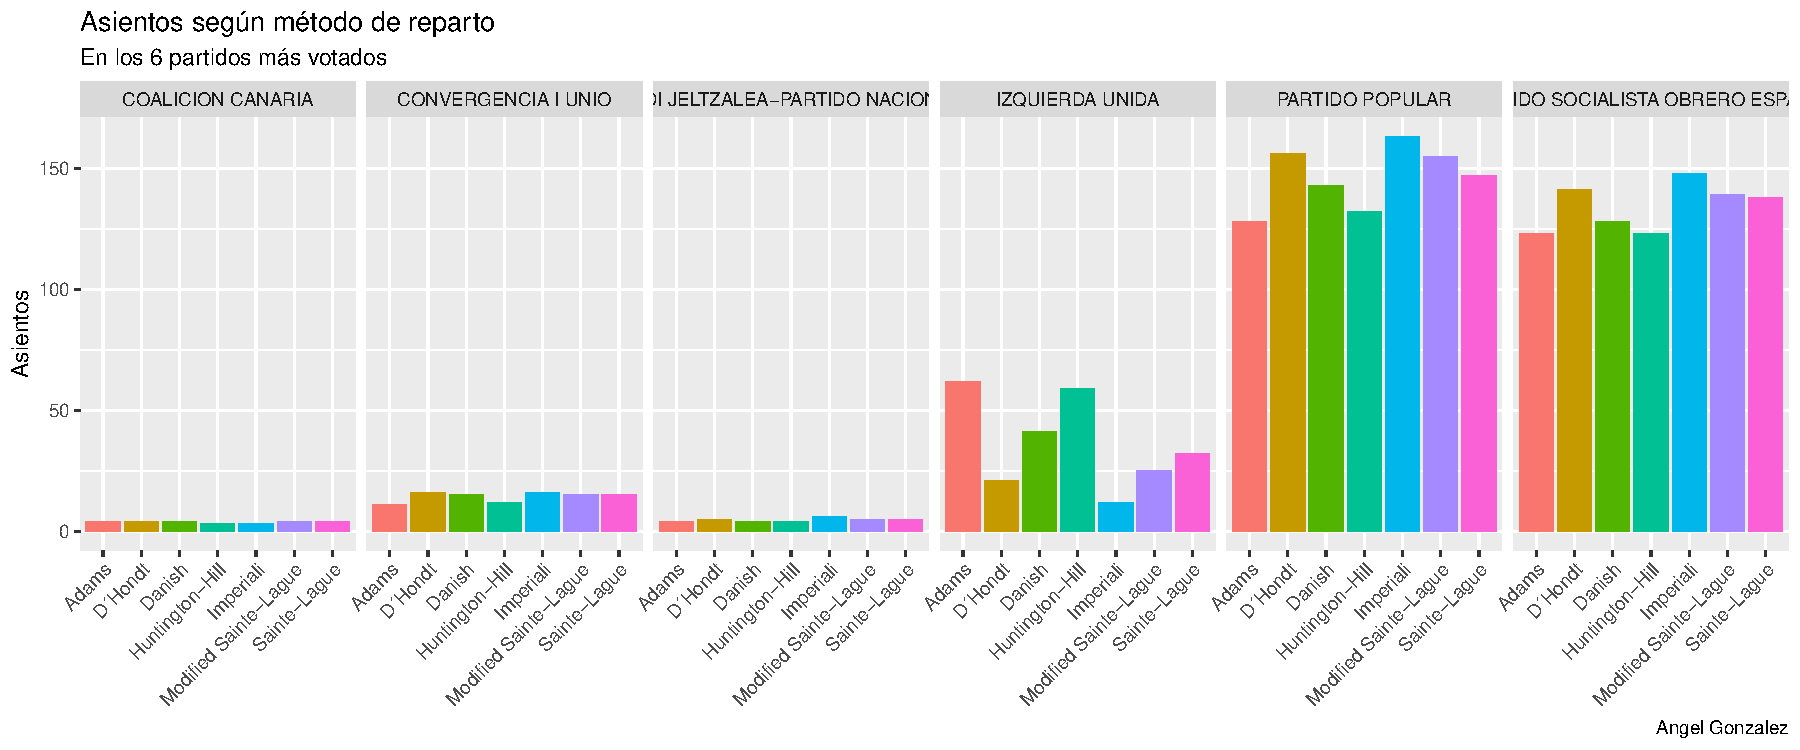
\includegraphics[width=0.95\linewidth]{figurasR/unnamed-chunk-64-1} \end{center}

En este caso únicamente modificamos el número de partidos presentes en
la elección, desde un único partido hasta 100 partidos que se presentan
a una elección ficticia.\\
Observamos que cuando se presentan de 2 a 25 partidos a las elecciones
la desproporción se encuentra en los máximos, disminuye a medida que se
presentan más partidos, alcanzando el mínimo de desproporción cuantos
más partidos se presenten a las elecciones.\\
Podemos apreciar en el gráfico que para un número bajo de partidos que
se presentan a las elecciones la variabilidad es alta pero decreciente,
a partir de los 25 partidos la variabilidad se estabiliza.\\
Concluimos que según el método LR-Imperiali obtenemos el mejor resultado
cuanto más partidos se presenten a las elecciones, empieza a presentar
una desproporción menor alrededor de los 50 partidos.

\hypertarget{lr-lmperiali-variando-la-concentraciuxf3n-del-voto}{%
\subsection{LR Lmperiali variando la concentración del
voto}\label{lr-lmperiali-variando-la-concentraciuxf3n-del-voto}}

\begin{center}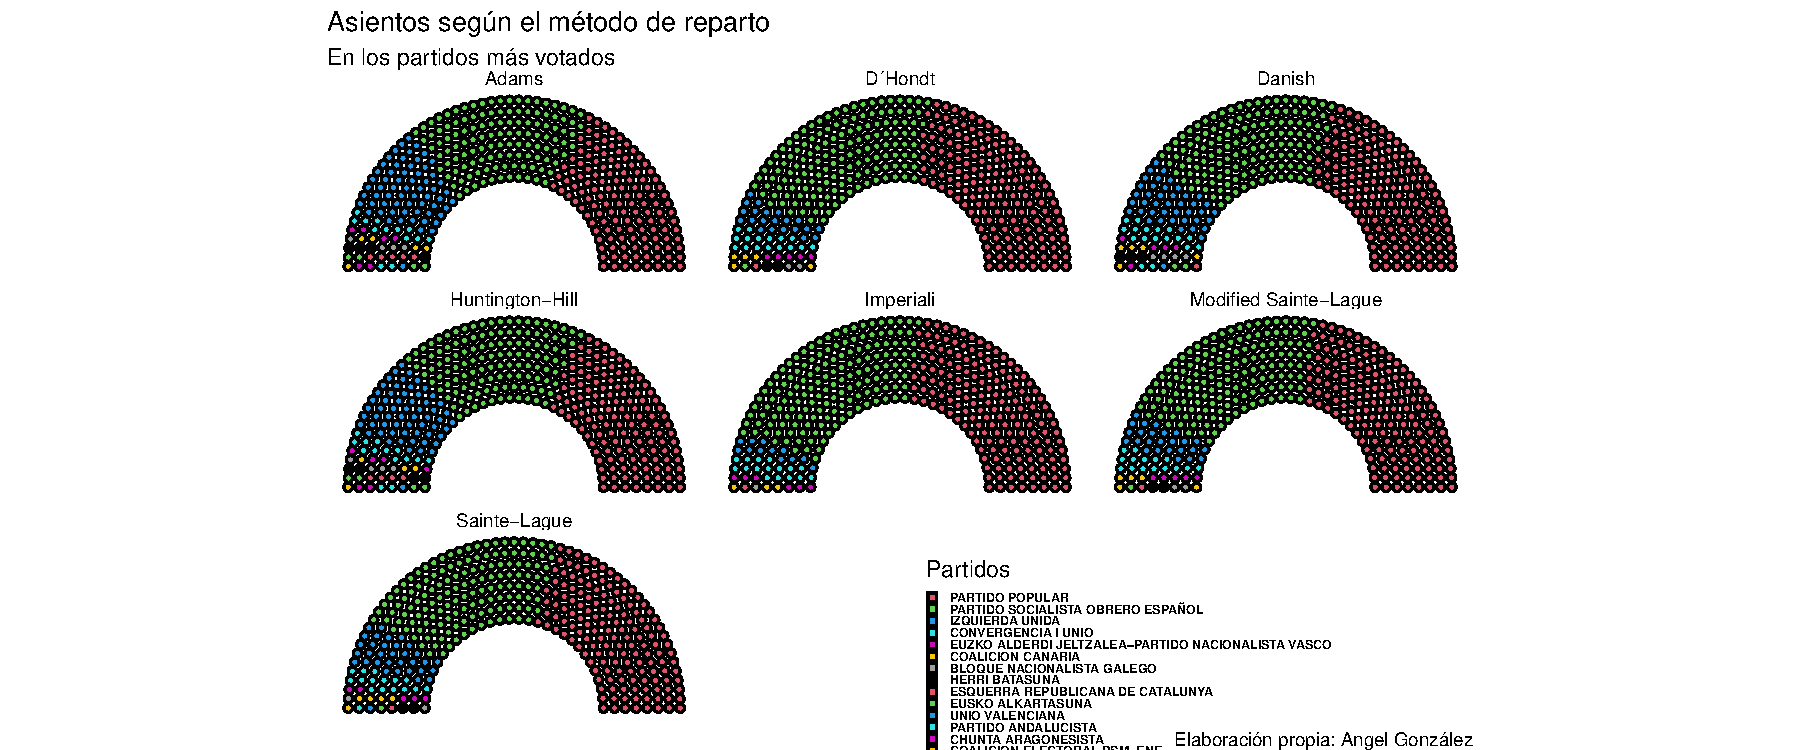
\includegraphics[width=0.95\linewidth]{figurasR/unnamed-chunk-65-1} \end{center}

En el presente gráfico variamos la concentración del voto en unas
elecciones ficticias, comenzamos con una concentración de votos baja, es
decir, la diferencia de votos entre partidos es baja, hasta acabar con
una concentración de votos alta, en donde la diferencia de votos entre
partidos es muy grande.\\
Observando el gráfico observamos que la desproporción está en un mismo
nivel ya se encuentre con una concentración de voto alta o baja. El
nivel de desproporción es muy bajo, por lo tanto muy deseable, con
valores muy cercanos a 0. Es un método que también presenta una buena
cualidad, puesto que su proporcionalidad es prácticamente
independientemente de la concentración del voto.

\hypertarget{comparaciones-entre-muxe9todos}{%
\section{Comparaciones entre
métodos}\label{comparaciones-entre-muxe9todos}}

En este apartado procederemos a agrupar todos los resultados de los
métodos utilizados anteriormente. El objetivo es ser capaces de comparar
en un mismo gráfico todos los métodos y sacar conclusiones. Se agruparán
los datos de los tres escenarios posibles, variando el número de
escaños, el número de partidos que se presentan a las elecciones o bien
la concentración de los votos entre los partidos.

Se recomiendan visitar los gráficos interactivos en la siguiente
dirección: \url{https://rpubs.com/angox/cap3int}

\hypertarget{variando-el-nuxfamero-de-escauxf1os}{%
\subsection{Variando el número de
escaños}\label{variando-el-nuxfamero-de-escauxf1os}}

\begin{center}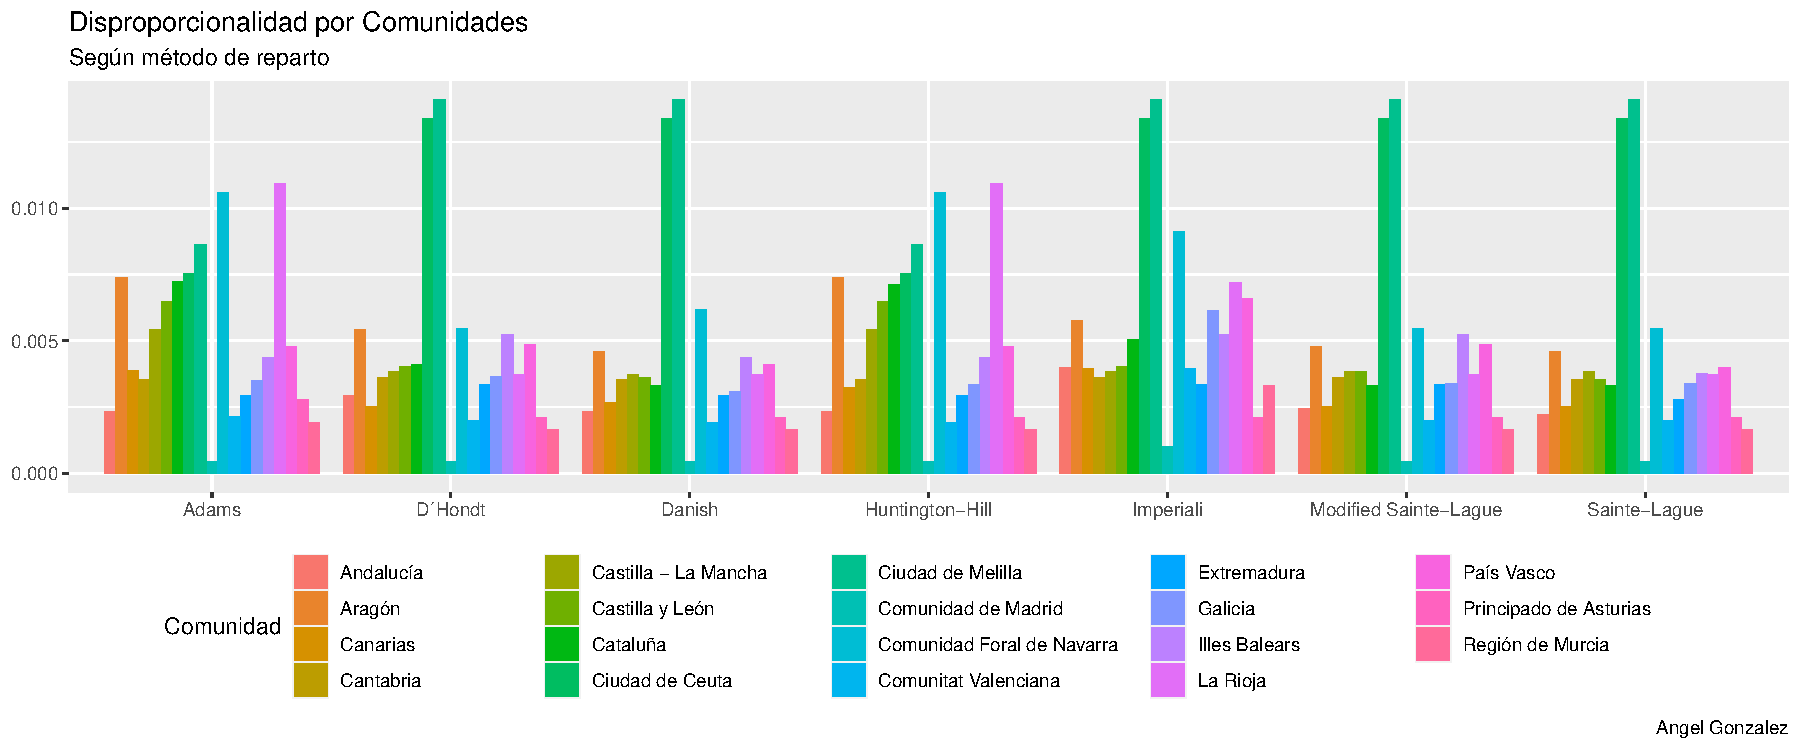
\includegraphics[width=0.95\linewidth]{figurasR/unnamed-chunk-66-1} \end{center}

En el presente gráfico comparamos en un mismo lugar los métodos
anteriormente analizados individualmente.\\
En esta comparación podemos observar que para todos los métodos a pocos
escaños a repartir la desproporción es muy alta y no hay casi diferencia
entre métodos, la desproporción baja cuanto mayor número de escaños a
repartir, a números muy altos de escaños la desproporción está muy
cercana al 0 y casi no hay diferencia de desproporción entre métodos.\\
El peor método en este caso es el Imperiali, que presenta una curva con
un descenso mucho más lento que los demás métodos. Todos los demás
métodos presentan un comportamiento similar.

\begin{center}\includegraphics[width=0.95\linewidth]{figurasR/unnamed-chunk-67-1} \end{center}

En este gráfico nos centramos en la desproporción para un número de
escaños a repartir de entre 300 y 400 diputados, actualmente en España
se reparten 350 diputados. El peor método entre los presentados es el
método Imperiali, con una diferencia significativa respecto a los demás
métodos. Podemos agrupar los métodos en dos grupos,un grupo que sería el
de una desproporción alta, en el que se encontrarían los métodos de
Imperiali, Adams y D´Hondt. Un segundo grupo que sería el que
presentaría una desproporción baja o media, con los restantes métodos.

Actualmente en España se reparten 350 escaños y se utiliza el método
D´Hondt, según los datos obtenidos podemos concluir que no es el mejor
método que se puede utilizar, es un método que está en el grupo de
desproporción alta, e incluso no es siempre el mejor método dentro de
ese subgrupo, sería interesante según lo observado en la gráfica
plantearse un cambio de método a otro mejor, al menos, a alguno dentro
del subgrupo de desproporción baja, preferentemente el mejor método que
podríamos utilizar dentro de los métodos de promedio mayor, que sería el
método de Sainte-Lague sin modificar. Hay que tener en cuenta también
que debido a que en España no se reparten los 350 diputados por
circunscripción única las conclusiones cambiarían levemente. En el caso
de que se repartan de 1 a 20 escaños el método D´Hont sigue sin ser uno
de los mejores métodos, pero su desproporción es muy similar a los demás
métodos por lo que hace al método D´Hont aceptable cuando se trata de
repartir pocos escaños.

\hypertarget{variando-el-nuxfamero-de-partidos}{%
\subsection{Variando el número de
partidos}\label{variando-el-nuxfamero-de-partidos}}

\begin{center}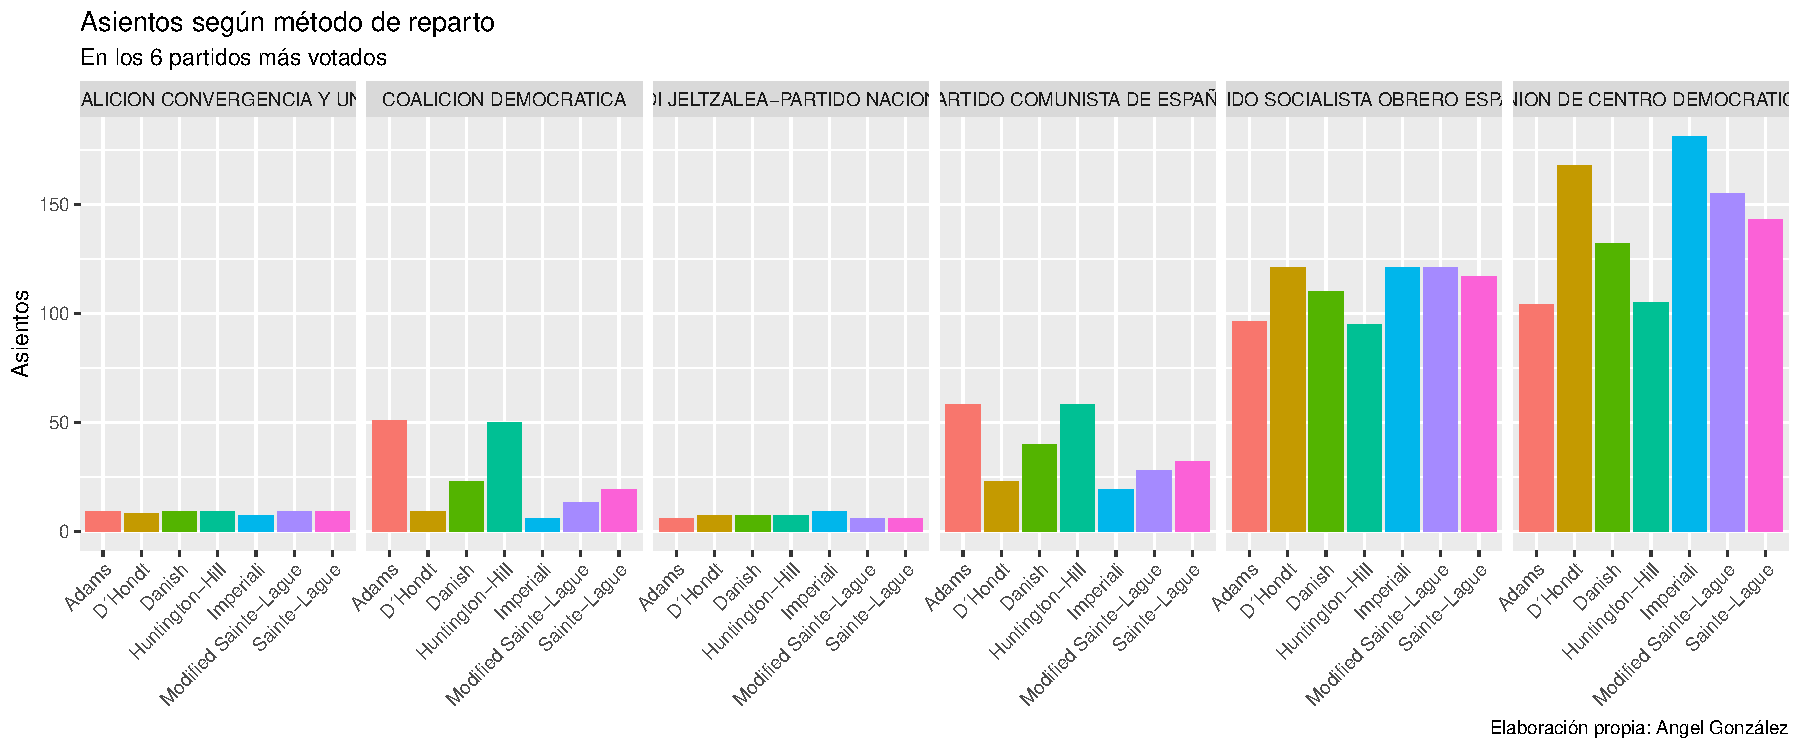
\includegraphics[width=0.95\linewidth]{figurasR/unnamed-chunk-68-1} \end{center}

En el presente gráfico comparamos la desproporción variando el número de
partidos en un mismo lugar con los métodos anteriormente analizados
individualmente.

Observamos que para un número de partidos bajo hasta los 25 partidos que
se presentan a unas elecciones la desproporción es muy variable, a
partir de los 25 partidos se estabiliza y podemos sacar algunas
conclusiones, en primer lugar los peores métodos claramente son en este
caso los métodos Adams y Huntington-Hill, mientras que los demás métodos
son similares en su desproporción, donde la menor desproporción la
podemos encontrar entre los métodos Sainte-Lague y LR-Hare. A
continuación nos centraremos en la desproporción cuando se presentan
pocos partidos para analizarlo más detenidamente.

\begin{center}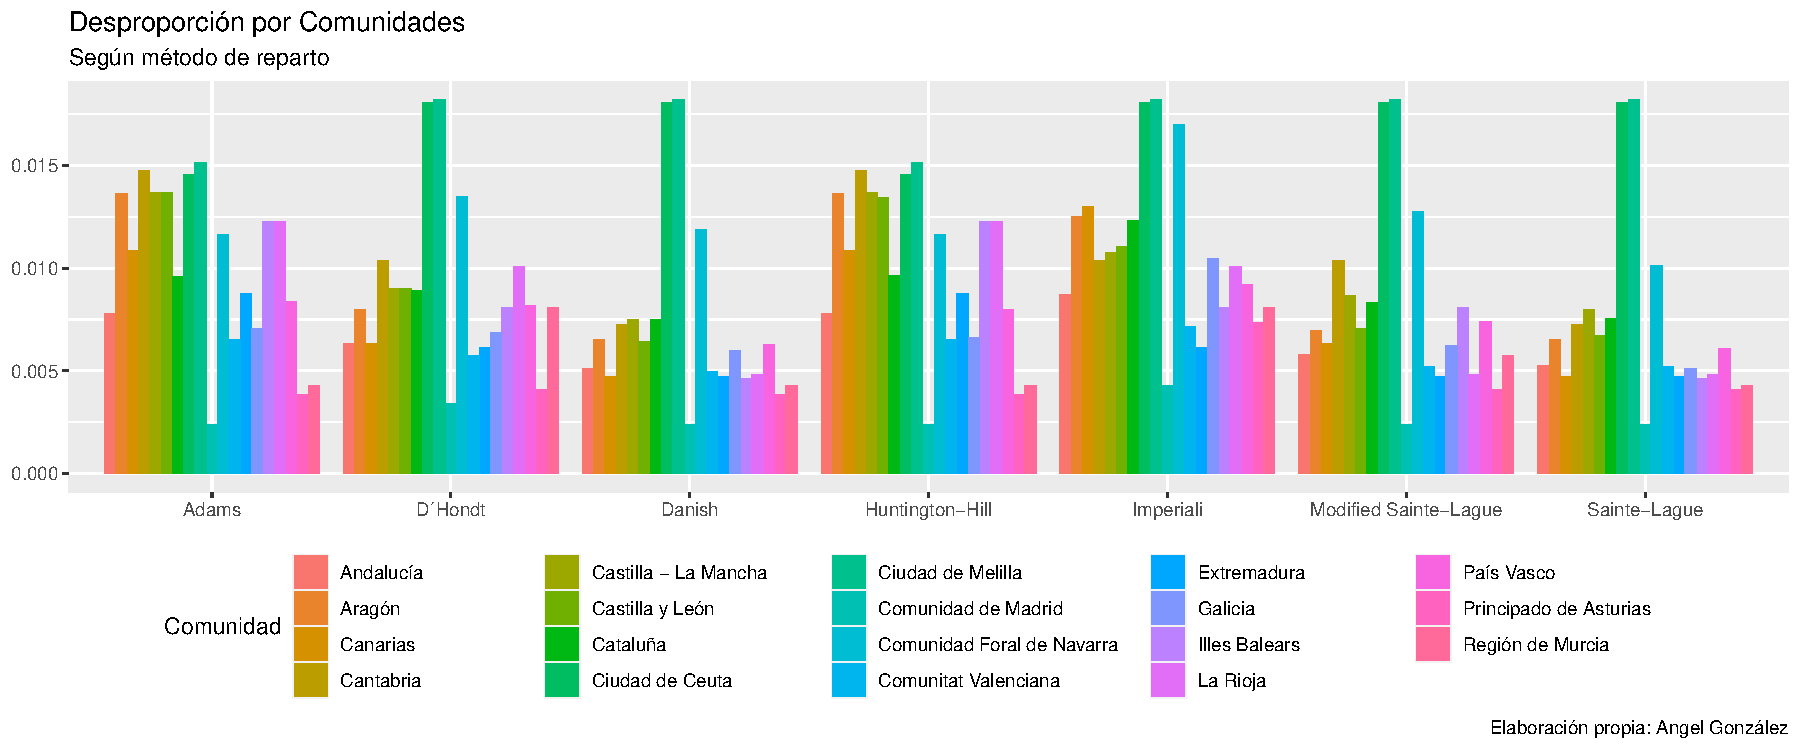
\includegraphics[width=0.95\linewidth]{figurasR/unnamed-chunk-69-1} \end{center}

En este gráfico nos centramos en la desproporción para un número de
partidos entre 2 y 50 partidos.

Observamos que hasta los 20 partidos que se presentan a las elecciones
la desproporción es muy variable entre ellos, a partir de los 20
partidos que se presentan en las elecciones podemos extraer algunas
conclusiones, se ven dos grupos diferenciados, un grupo en donde la
desproporción es estable e incluso decreciente y otro grupo en el que la
desproporción va aumentando, que son los métodos de Adams y
Huntington-Hill.\\
En España se utiliza el método D´Hondt, según los datos obtenidos
podemos concluir que el método d´Hondt no es el mejor método entre los
analizados, se encontraría en un nivel medio-alto entre los métodos
posibles, es decir, sería deseable para obtener una mayor
proporcionalidad que se cambiase el método de reparto a otro mejor, en
este caso observamos que el mejor método dentro del grupo de promedios
mayores es el Saint-Lague y dentro del grupo de resto mayor el mejor
parado es el método LR-Hare.

\hypertarget{variando-la-concentraciuxf3n-del-voto}{%
\subsection{Variando la concentración del
voto}\label{variando-la-concentraciuxf3n-del-voto}}

\begin{center}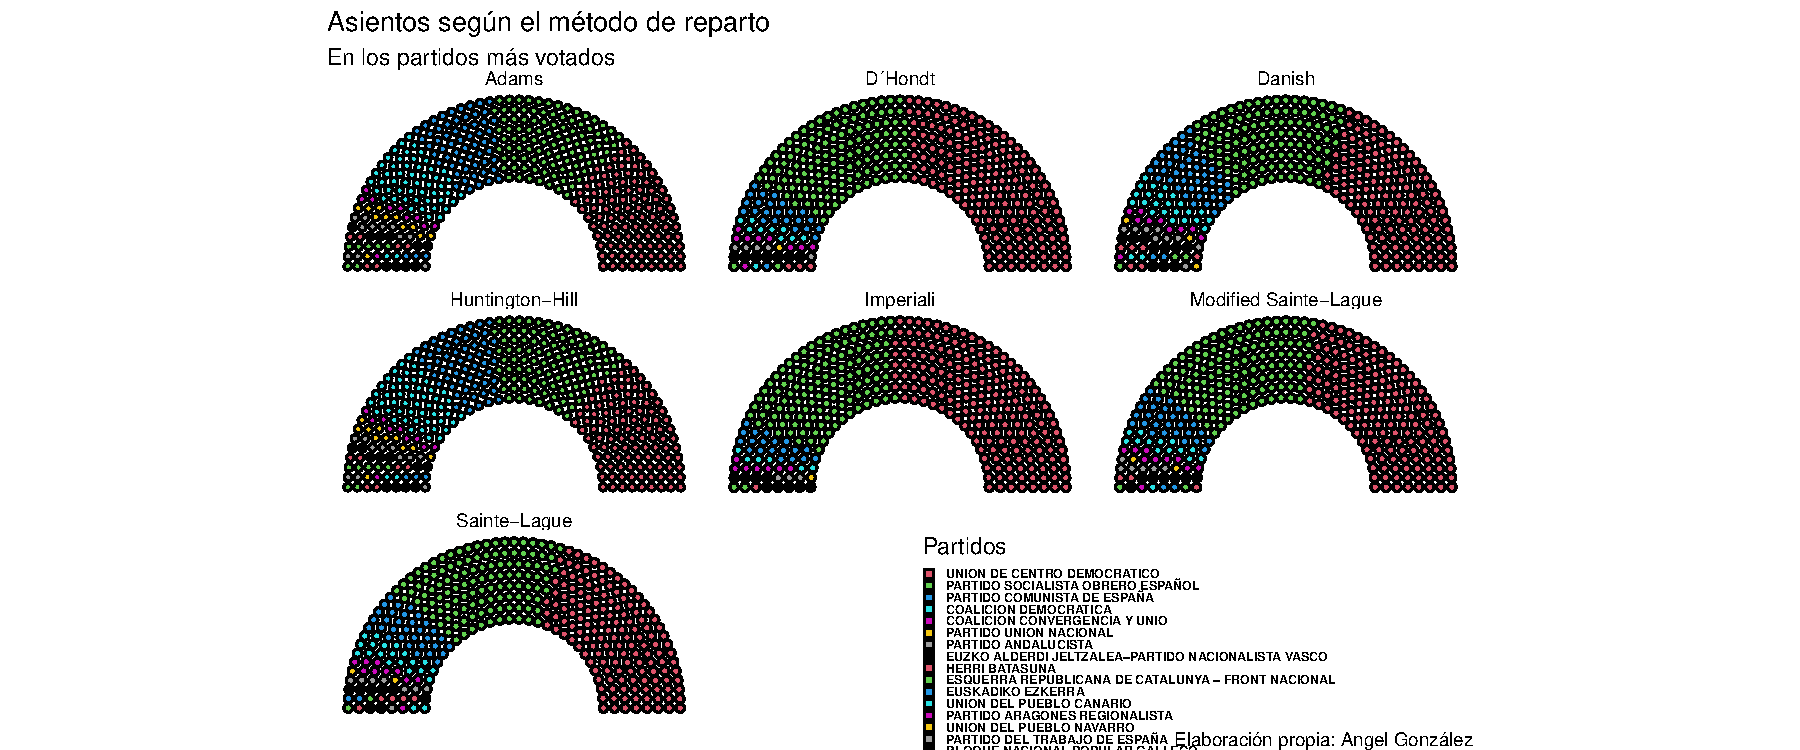
\includegraphics[width=0.95\linewidth]{figurasR/unnamed-chunk-70-1} \end{center}

En el presente gráfico comparamos la concentración del voto en unas
elecciones ficticias, comenzamos con una concentración de votos baja, es
decir, la diferencia de votos entre partidos es baja, hasta acabar con
una concentración de votos alta, en donde la diferencia de votos entre
partidos es muy grande. Todo ello en un mismo lugar con los métodos
anteriormente analizados individualmente.

Observamos que hay dos grupos diferenciados, uno de ellos en los que la
desproporción es baja para una menor concentración de votos entre los
partidos y que a medida que la concentración aumenta también va
aumentando la desproporción, donde se encuentran los métodos de Adams y
Huntington-Hill, también se comporta así el método Imperiali hasta una
concentración de votos media. El otro grupo se caracteriza por ya sea la
concentración del voto muy baja o muy alta, la desproporción está en un
nivel bajo y no varía significativamente.

\begin{center}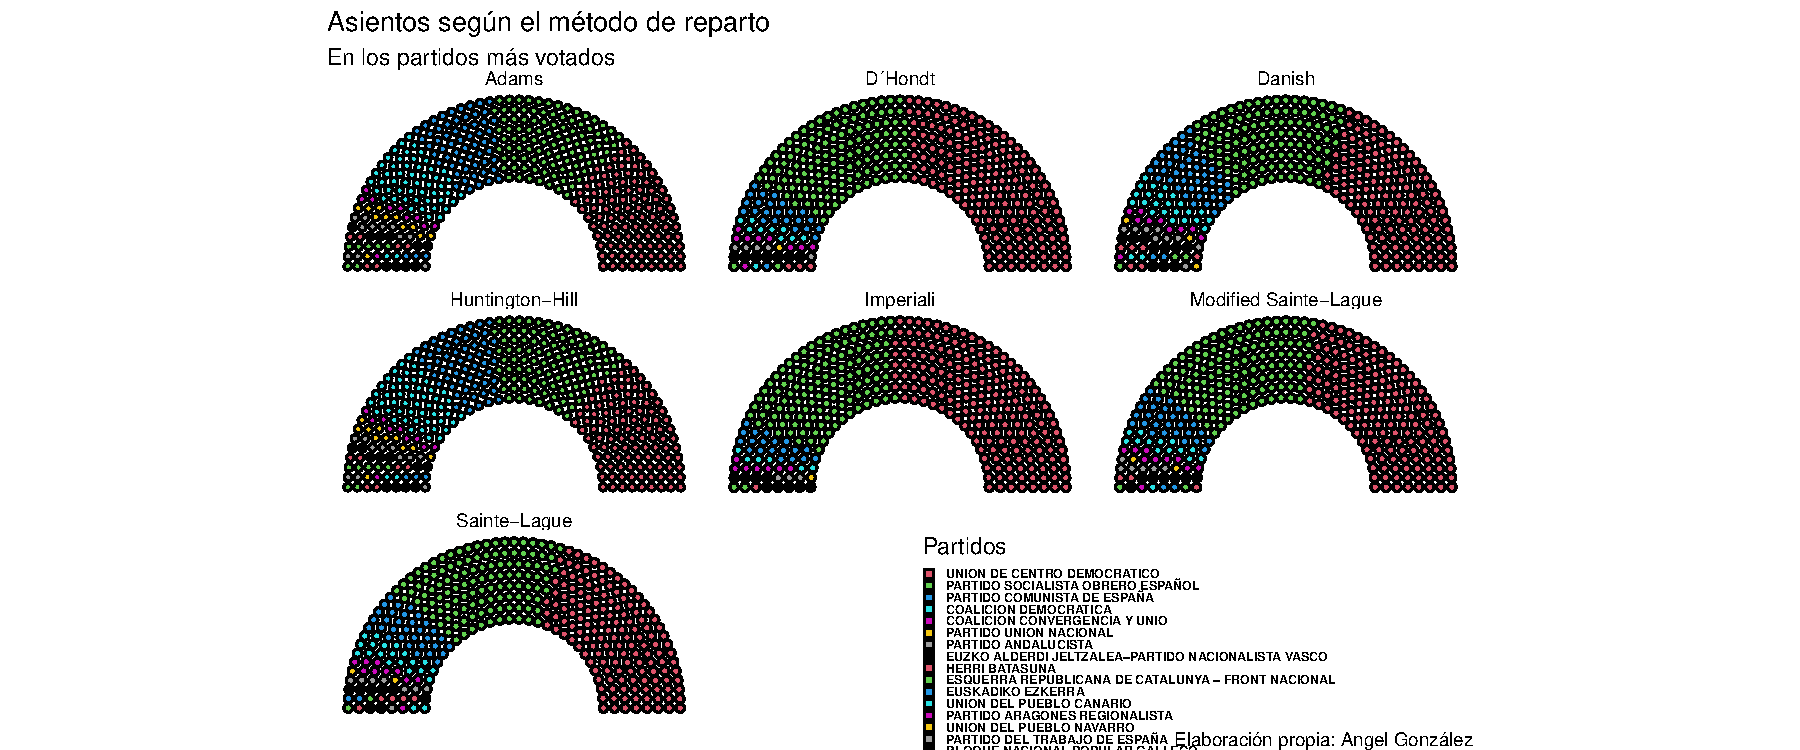
\includegraphics[width=0.95\linewidth]{figurasR/unnamed-chunk-71-1} \end{center}

En este gráfico nos centramos en los casos en que hay mayor
concentración de votos de unos pocos partidos, lo que suele suceder
habitualmente.\\
Vemos que hay dos grupos diferenciados, uno en el que hay una alta
desproporción, que serían los métodos Imperiali, Adams, D´Hondt y
Huntington-Hill y otro en el que la desproporción es baja. En España, la
concentración de voto suele ser alta o medio-alta y se utiliza como
método de reparto el método D´Hondt, por lo tanto observando el gráfico
podemos decir que el método utilizado en España no es el más óptimo si
se busca obtener un bajo índice de desproporción, sería conveniente
realizar un cambio de método y cambiar el método D´Hondt preferentemente
por el método Sainte-Lague o Danish, que son los mejores entre los
métodos del grupo de promedio mayor con desproporción baja. Dentro del
grupo de los métodos de resto mayor todos ellos se comportan con una
desproporción muy baja.

\hypertarget{gruxe1ficos-3d}{%
\section{Gráficos 3D}\label{gruxe1ficos-3d}}

\begin{figure}[H]

{\centering 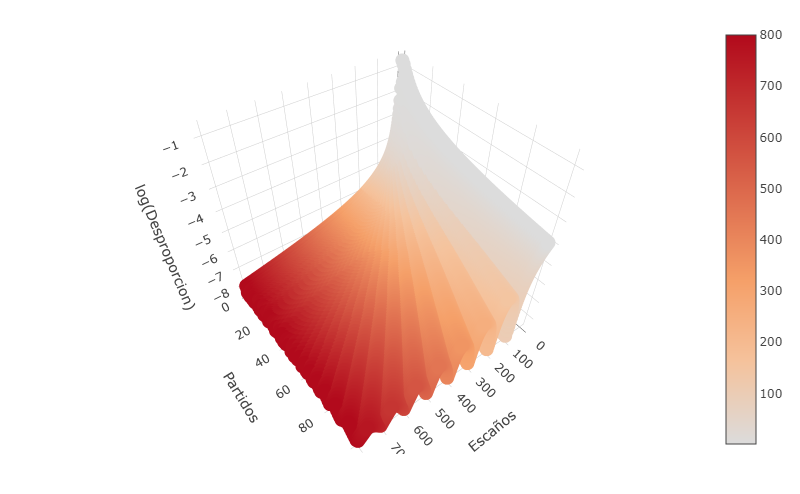
\includegraphics[width=0.95\linewidth]{graficos/dont_despro_bajo} 

}

\caption{Método 3D D´Hondt}\label{fig:graf3d}
\end{figure}

En este apartado se ha realizado un gráfico 3D para cada método, en
donde se han modificado a la vez tanto el número de partidos como el
número de escaños. Se han realizado tres gráficos distintos dentro de
cada método, para una concentración del voto alta, media o baja.

Debido a la lentitud en el cálculo únicamente generaremos el gráfico
para el método D´Hondt, se ha procedido de la siguiente manera, en
primer lugar se han calculado los datos en \emph{3dplotly.Rmd}, el cual
guarda los datos en la carpeta Datos/3dData. Una vez obtenidos los datos
generamos los gráficos interactivos en \emph{cap3Dmetodos.Rmd}. El
código para los demás métodos se encuentran en ambos archivos
comentados. La dirección para acceder a los gráficos interactivos es
\url{https://rpubs.com/angox/graf3D}

\hypertarget{conclusiones}{%
\section{Conclusiones}\label{conclusiones}}

En general podemos concluir que una vez comparados todos los métodos
tanto modificando el número de escaños a repartir, en número de partidos
que se presentan a la elección y la concentración de los votos,
concluimos que los mejores métodos dentro del grupo de promedios mayores
son en primer lugar el método Saint-Lague, seguido por el Modified
Sainte-Lague y el Danish. En el caso del método utilizado actualmente en
España, el método D´hondt, podemos decir que es un método que no siendo
de los peores se queda en un nivel medio, es decir, que no es un método
que se debiese usar si lo que se busca es obtener el máximo nivel de
proporcionalidad, no es el mejor en ninguno de las posibles
modificaciones que se presentan en este estudio, siendo entonces
conveniente para España cambiar el método de reparto de escaños y
utilizar dentro del grupo de promedios mayores el método de Sainte-Lague
que es el que consistentemente ha presentado los mejores resultados.
Entre los métodos de resto mayor todos ellos presentan un comportamiento
muy similar por lo que podría utilizarse cualquiera de ellos.

\FloatBarrier

\ifdefined\ifprincipal
\else
\setlength{\parindent}{1em}
\pagestyle{fancy}
\setcounter{tocdepth}{4}
\tableofcontents

\fi

\ifdefined\ifdoblecara
\fancyhead{}{}
\fancyhead[LE,RO]{\scriptsize\rightmark}
\fancyfoot[LO,RE]{\scriptsize\slshape \leftmark}
\fancyfoot[C]{}
\fancyfoot[LE,RO]{\footnotesize\thepage}
\else
\fancyhead{}{}
\fancyhead[RO]{\scriptsize\rightmark}
\fancyfoot[LO]{\scriptsize\slshape \leftmark}
\fancyfoot[C]{}
\fancyfoot[RO]{\footnotesize\thepage}
\fi
\renewcommand{\headrulewidth}{0.4pt}
\renewcommand{\footrulewidth}{0.4pt}

\hypertarget{elecciones-espauxf1olas-seguxfan-distintos-muxe9todos-de-reparto-de-escauxf1os}{%
\chapter{Elecciones españolas según distintos métodos de reparto de
escaños}\label{elecciones-espauxf1olas-seguxfan-distintos-muxe9todos-de-reparto-de-escauxf1os}}

A continuación analizaremos el reparto de escaños para el congreso de
las distintas elecciones en España desde el 1977. Aplicando diferentes
métodos de reparto de escaños, analizaremos los resultados obtenidos en
cada elección. Una vez obtenido el reparto de escaños según los
distintos métodos procederemos a obtener la proporcionalidad para cada
método y así analizar la desproporción tanto por comunidades autónomas
como por España en su conjunto.

\hypertarget{procedimiento-1}{%
\section{Procedimiento}\label{procedimiento-1}}

Para ser capaces de realizar el análisis pretendido se ha procedido de
este modo:

\begin{itemize}
\tightlist
\item
  En primer lugar se han obtenido los resultados de las elecciones al
  congreso de la página web del ministerio del interior\footnote{\href{http://www.infoelectoral.mir.es/min/}{Consulta
    de resultados electorales Ministerio del interior}}, desde el año
  1977 hasta las últimas elecciones del 2019.
\end{itemize}

\begin{itemize}
\tightlist
\item
  Creación de las distintas funciones para los distintos métodos de
  reparto de escaños así como la función para calcular la desproporción.
  Se han empleado distintas librerías de \emph{R} tal y como
  \emph{openxlsx} para leer los diferentes resultados electorales,
  \emph{electoral} como apoyo para escribir las funciones,
  \emph{data.table}, \emph{dplyr} y \emph{tidyr} para manipular los
  datos, \emph{ggplot2} y \emph{ggpol} para la creación de los distintos
  gráficos. Como muestra se presenta la función para el método D´Hondt:
\end{itemize}

\pagebreak

\begin{Shaded}
\begin{Highlighting}[]
\NormalTok{asientos\_dhondt }\OtherTok{\textless{}{-}} \ControlFlowTok{function}\NormalTok{(partidos, votos,}
\NormalTok{                            n\_escannos,}
                            \AttributeTok{couta\_min =} \DecValTok{0}\NormalTok{) \{}
  \CommentTok{\# Cuota mínima}
\NormalTok{  nv }\OtherTok{\textless{}{-}} \FunctionTok{sum}\NormalTok{(votos)}
\NormalTok{  vn }\OtherTok{\textless{}{-}}\NormalTok{ votos}
\NormalTok{  vn[votos }\SpecialCharTok{\textless{}=}\NormalTok{ nv }\SpecialCharTok{*}\NormalTok{ couta\_min] }\OtherTok{\textless{}{-}} \DecValTok{0}
\NormalTok{  votos }\OtherTok{\textless{}{-}}\NormalTok{ vn}

  \CommentTok{\# Escaños}
\NormalTok{  div }\OtherTok{\textless{}{-}} \DecValTok{1}\SpecialCharTok{:}\NormalTok{n\_escannos}
\NormalTok{  G }\OtherTok{\textless{}{-}} \FunctionTok{sapply}\NormalTok{(div, }\ControlFlowTok{function}\NormalTok{(x) votos }\SpecialCharTok{/}\NormalTok{ x)}
\NormalTok{  cuota }\OtherTok{\textless{}{-}}\NormalTok{ G[}\FunctionTok{order}\NormalTok{(G, }\AttributeTok{decreasing =}\NormalTok{ T)][n\_escannos]}
\NormalTok{  W }\OtherTok{\textless{}{-}}\NormalTok{ (G }\SpecialCharTok{\textgreater{}=}\NormalTok{ cuota)}
\NormalTok{  seats }\OtherTok{\textless{}{-}} \FunctionTok{rowSums}\NormalTok{(W)}
\NormalTok{  o }\OtherTok{\textless{}{-}}\NormalTok{ seats}
  \CommentTok{\# Resultados}
  \FunctionTok{data.frame}\NormalTok{(}\StringTok{"Partidos"} \OtherTok{=}\NormalTok{ partidos, }\StringTok{"Escanos"} \OtherTok{=} \FunctionTok{as.numeric}\NormalTok{(o))}
\NormalTok{\}}
\end{Highlighting}
\end{Shaded}

\begin{itemize}
\item
  Una vez obtenidos los resultados electorales y creadas las funciones
  necesarias, se procede a aplicar las funciones creadas con los
  resultados electorales.
\item
  Creación de los gráficos y análisis de los resultados, tanto para el
  reparto de escaños como para los resultados de la desproporción por
  comunidades autónomas y España en su conjunto.
\end{itemize}

\newpage

\hypertarget{auxf1o-1977}{%
\section{Año 1977}\label{auxf1o-1977}}

\hypertarget{comparativa-de-asientos-obtenidos}{%
\subsection{Comparativa de asientos
obtenidos}\label{comparativa-de-asientos-obtenidos}}

\begin{center}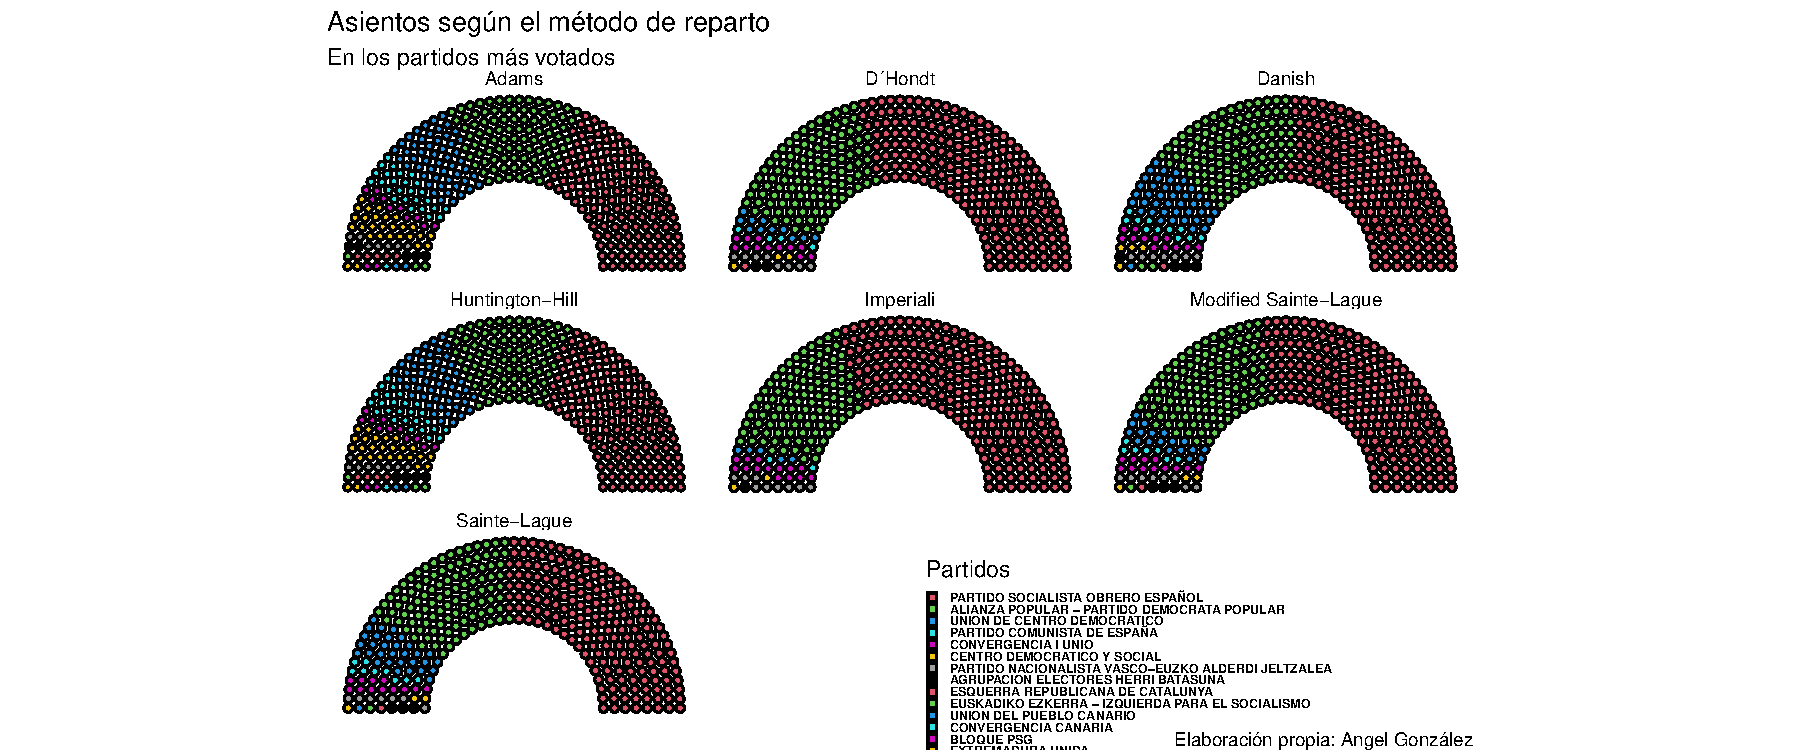
\includegraphics[width=1\linewidth]{figurasR/unnamed-chunk-78-1} \end{center}

En estas primeras elecciones de 1977 podemos observar que la fuerza más
votada en las elecciones es el partido \emph{Unión de Centro
democrático} seguido del \emph{PSOE}. Observamos que según el método
vigente en España, el método D´Hondt, el partido \emph{UCD}, que ganaría
las elecciones, tendría una gran diferencia de votos respecto a los
demás partidos, por lo que facilitaría la gobernanza.

Comparando entre métodos de reparto observamos que el que más escaños da
a los partidos grandes es el método Imperiali, que beneficia mucho a los
partidos más votados y penaliza mucho en escaños a los partidos tanto
medianos como poco votados. El método actual en España también tiene un
comportamiento similar al Imperiali aunque no tan acusado. En la otra
parte de la balanza nos encontramos con el método Adams, el cual da muy
pocos escaños al partido más votado y a los partidos medianos les
beneficia.

En estas elecciones no se obtiene la mayoría absoluta en ningún método
excepto en el método Imperiali, en los demás métodos el partido ganador
debería de aliarse con uno o más partidos para obtener la mayoría
absoluta, los grandes perdedores en términos de escaños obtenidos son el
partido comunista y Alianza Popular, que podrían obtener hasta 10
escaños más de haber optado por otro método de reparto de votos.

\hypertarget{desproporciuxf3n}{%
\subsection{Desproporción}\label{desproporciuxf3n}}

\begin{center}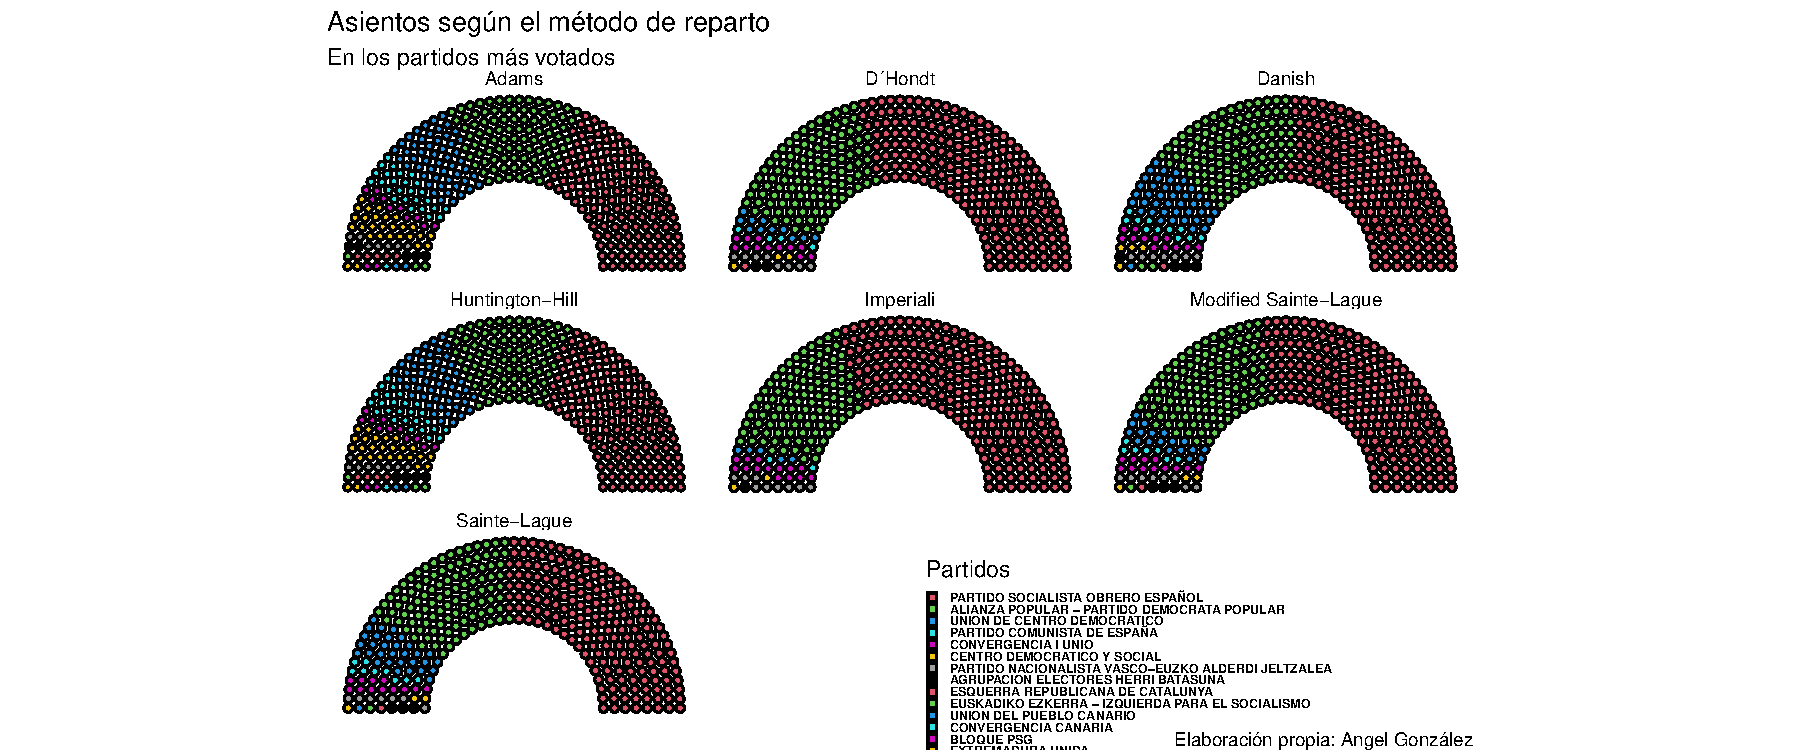
\includegraphics[width=1\linewidth]{figurasR/unnamed-chunk-79-1} \end{center}

\begin{center}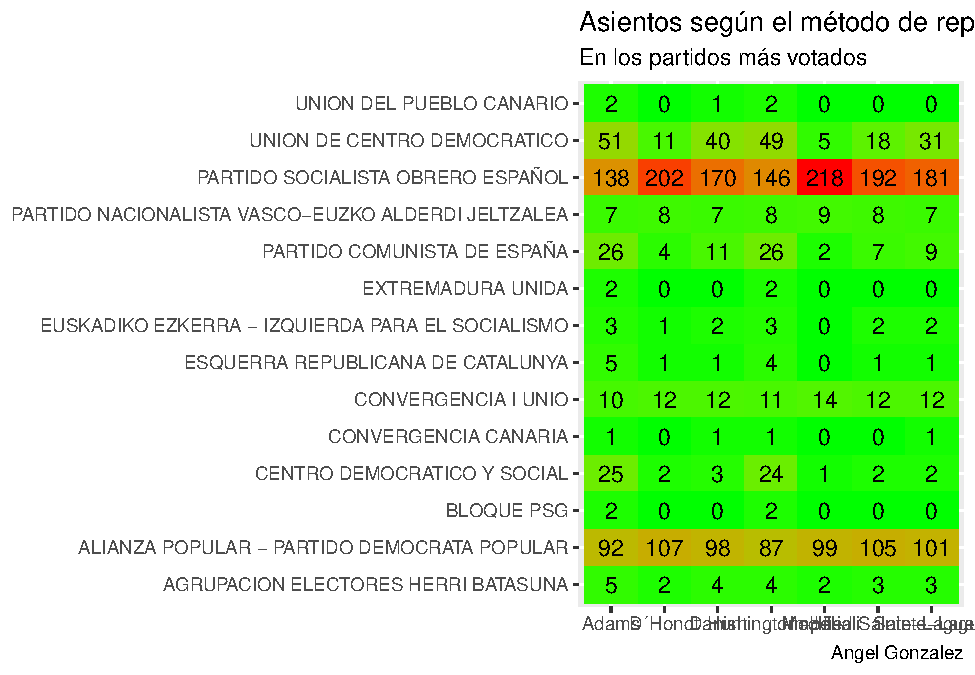
\includegraphics[width=1\linewidth]{figurasR/unnamed-chunk-79-2} \end{center}

En el presente gráfico, en el que se mide la desproporción por
comunidades, observamos que en general entre todos los métodos las
comunidades más desproporcionadas son las ciudades de Ceuta y Melilla,
resultado lógico en tanto que al repartirse un único escaño es el
partido más votado únicamente el que obtiene el escaño. Es común entre
todos los métodos que la comunidad de Madrid sea la comunidad más
proporcionada, esto es debido a que es la comunidad en la que se
reparten más asientos y también la más poblada, por lo que cuando se
reparten los asientos por provincias, al utilizar el método D´Hondt,
como hemos visto beneficia a los lugares con más población.\\
En general los métodos que presentan una menor diferencia de
desproporción entre las distintas comunidades autónomas son el método
Danish, LR-Hare y el Saint-Lague, en cambio las que presentan una mayor
diferencia entre comunidades son el método Imperiali, Adams y el
Huntington-Hill.

Si nos centramos en el gráfico de la desproporción media según el método
de reparto podemos observar que la menor desproporción se encuentra en
los métodos LR-Hare, Danish y Sainte-Lague, mientras que la mayor
desproporción se encuentran en el método Imperiali y Adams. Especial
caso hacemos al método D´Hondt al ser el método utilizado actualmente en
España, observamos que ni es el mejor método ni tampoco es de los
peores, debido a ello sería conveniente cambiar el método de reparto a
otro mejor, que podría ser o bien el Sainte-Lague, LR-Hare o el Danish.

\hypertarget{auxf1o-1979}{%
\section{Año 1979}\label{auxf1o-1979}}

\hypertarget{comparativa-de-asientos-obtenidos-1}{%
\subsection{Comparativa de asientos
obtenidos}\label{comparativa-de-asientos-obtenidos-1}}

\begin{center}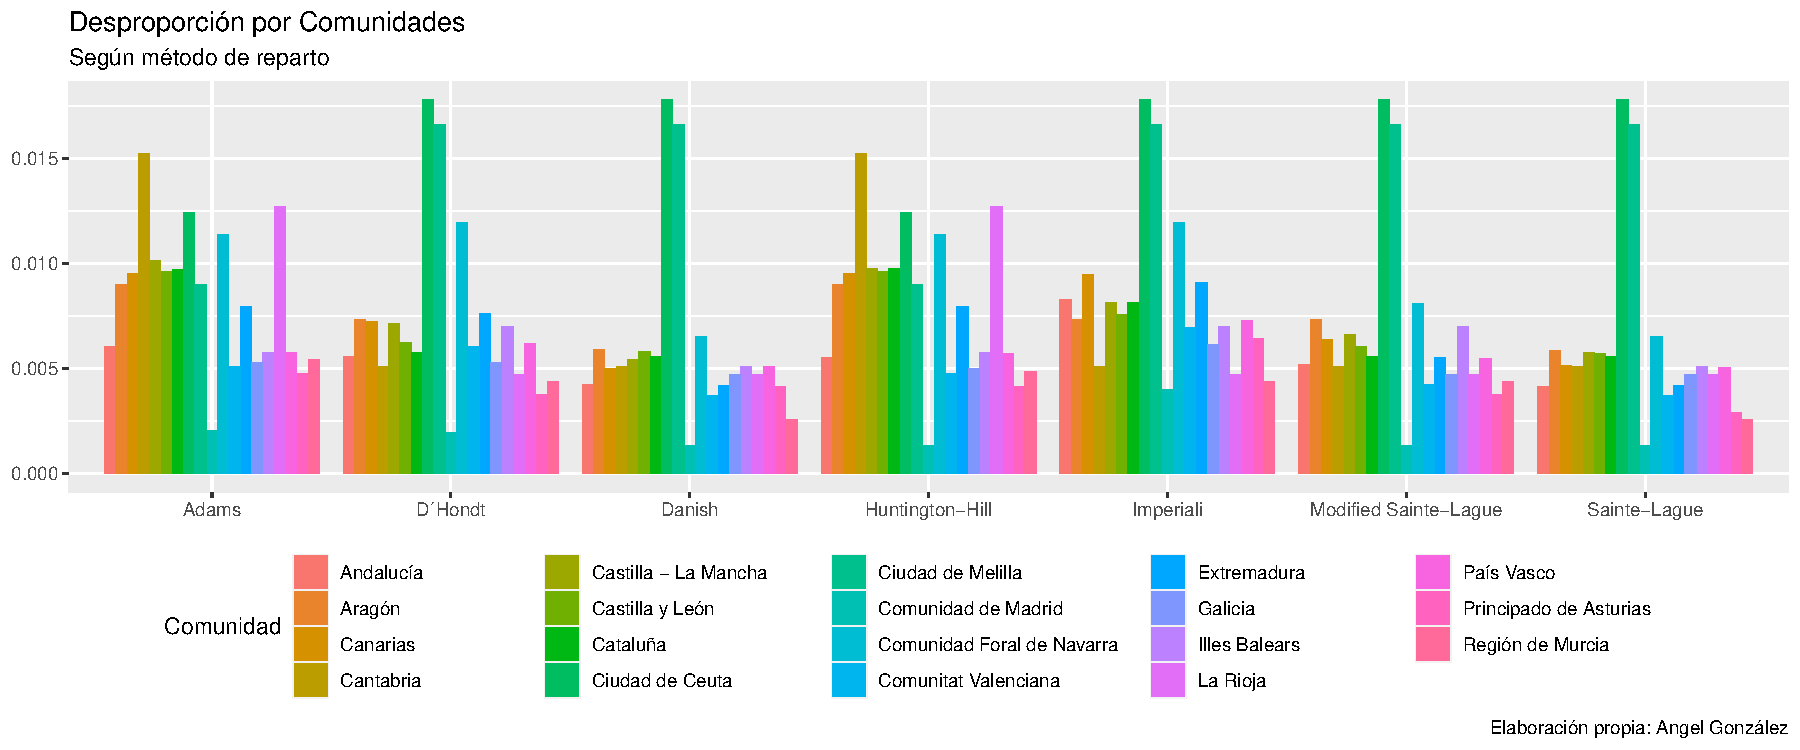
\includegraphics[width=1\linewidth]{figurasR/unnamed-chunk-81-1} \end{center}

En estas elecciones de 1979 el partido más votado fue \emph{UCD} seguido
del \emph{PSOE}, según los distintos métodos de reparto únicamente en el
método Imperiali \emph{UCD} conseguiría la mayoría absoluta, en todos
los demás métodos de reparto no se alcanza la mayoría absoluta, los
partidos más castigados por utilizar el método D´Hondt son el partido
comunista y coalición Democrática, que podrían hasta doblar el número de
asientos obtenidos dependiendo del método de reparto que se haya
realizado. En estas elecciones podemos decir que hay dos grandes
partidos y dos medianos, UCD y el PSOE son los más grandes y el partido
comunista y coalición democrática son los partidos medianos, después ya
se encuentran todos los demás.

\hypertarget{desproporciuxf3n-1}{%
\subsection{Desproporción}\label{desproporciuxf3n-1}}

\begin{center}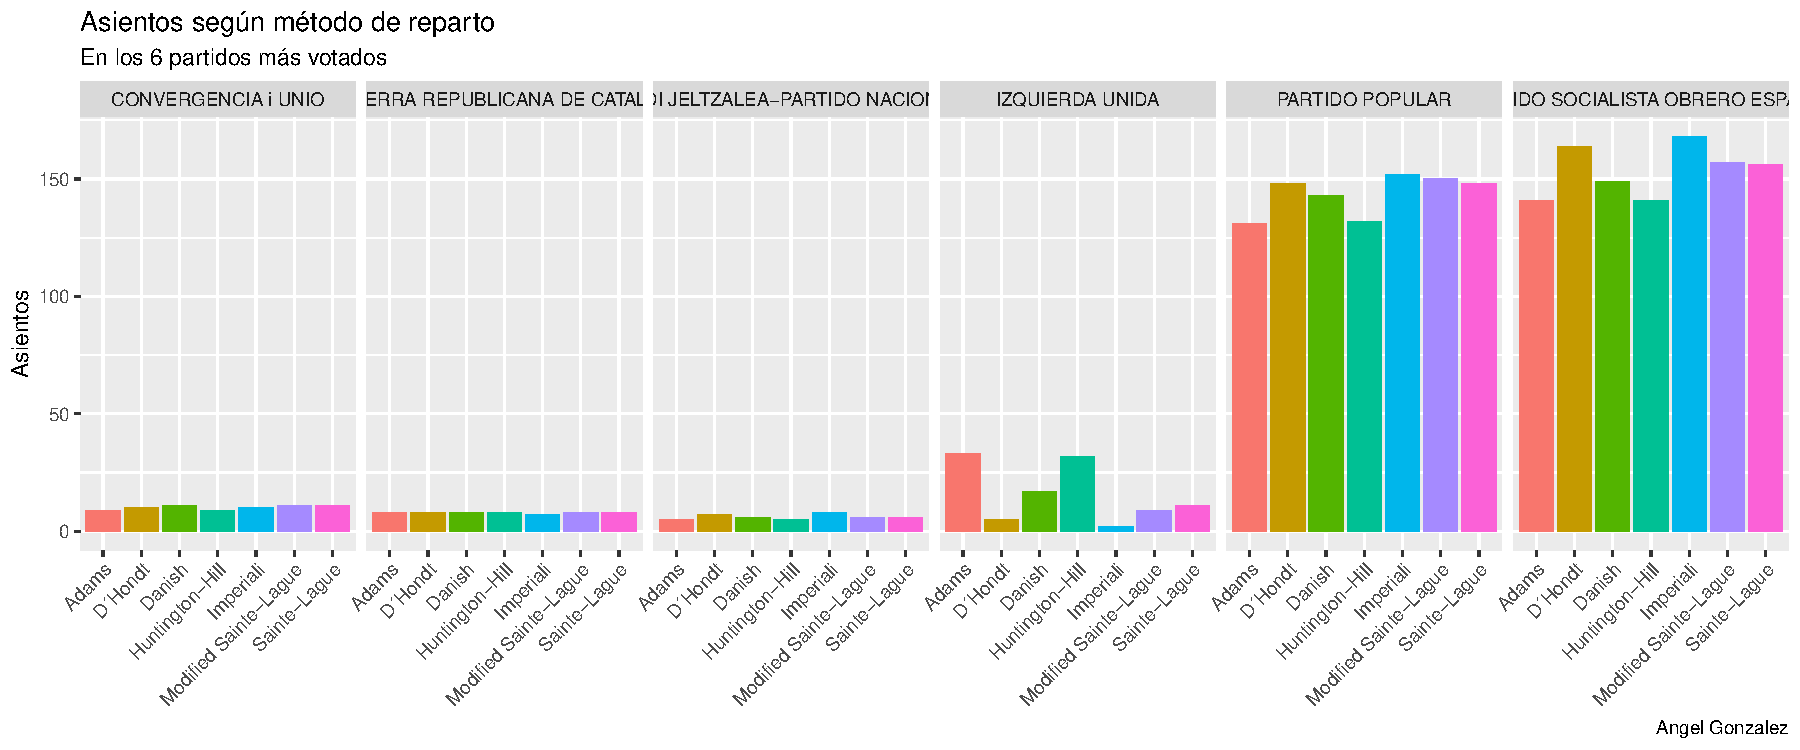
\includegraphics[width=1\linewidth]{figurasR/unnamed-chunk-82-1} \end{center}

\begin{center}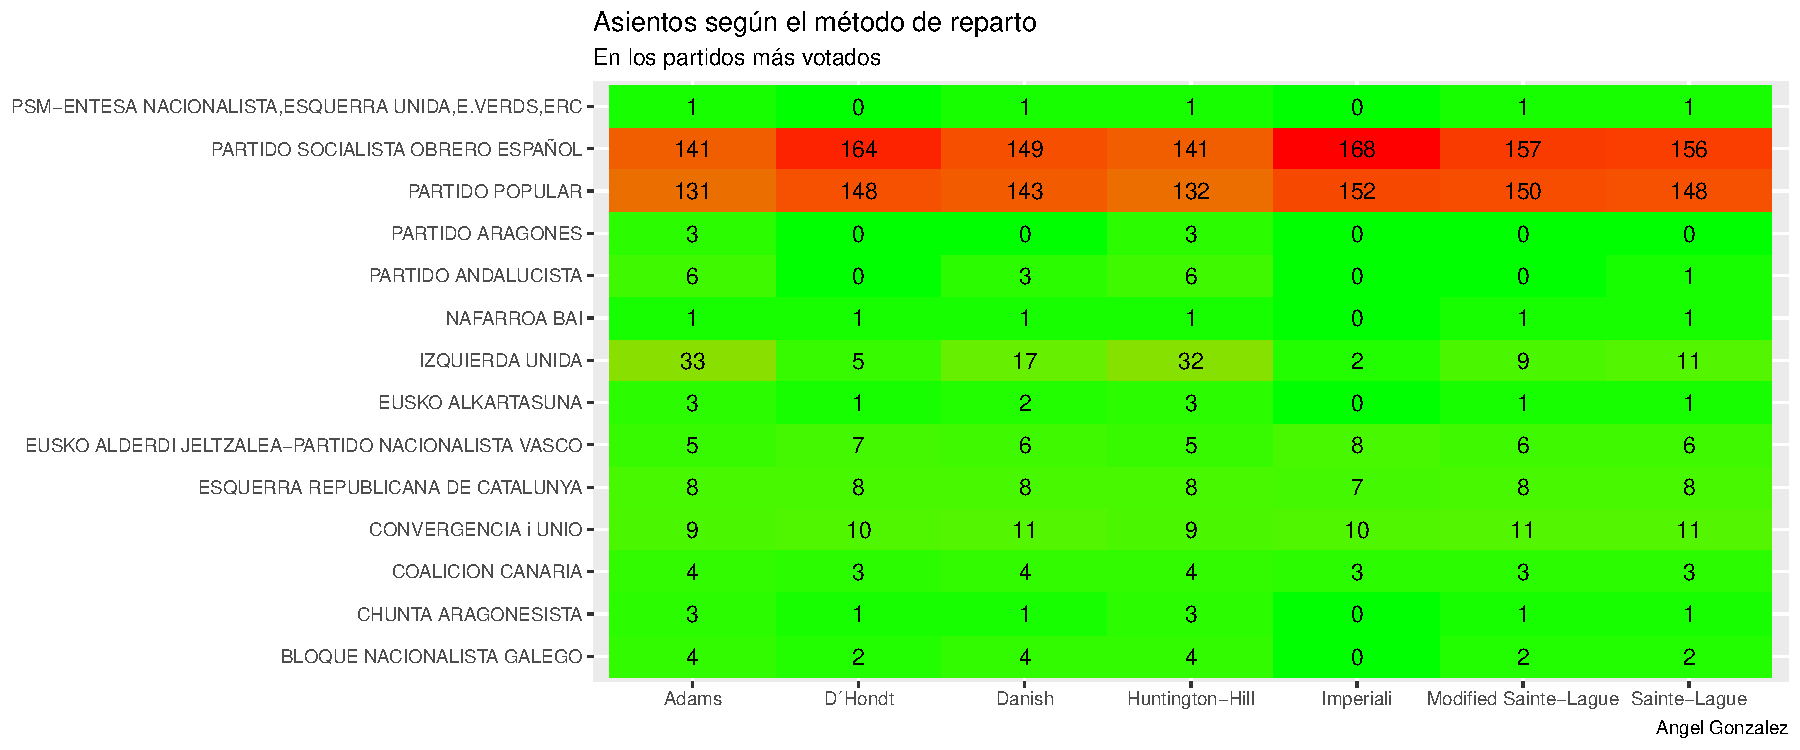
\includegraphics[width=1\linewidth]{figurasR/unnamed-chunk-82-2} \end{center}

En el presente gráfico vemos como respecto a las anteriores elecciones
hay una mayor diferencia de desproporción entre comunidades, las
ciudades de Ceuta y Melilla siguen presentando la mayor desproporción
como es habitual y la comunidad de Madrid la menor desproporción. El
comportamiento de la desproporción en las comunidades se puede agrupar
en dos grupos, un grupo compuesto por los métodos Imperiali,
Huntington-Hill y Adams, y otro grupo con los restantes métodos.

Según la desproporción media los peores métodos de reparto se pueden
agrupar en un grupo de tres métodos, el método Imperiali,
Huntington-Hill, y el Adams. Entre los mejores métodos de reparto se
encuentran el LR-Hare, Danish y el Sainte-Lague. En el caso del método
D´Hondt se encuentra en un término medio más próximo a los métodos más
desproporcionados, por lo que sería conveniente cambiar el método de
reparto a uno más proporcional, como puede ser el Danish o el
Sainte-Lague dentro de los métodos de promedio mayor o bien por el
LR-Hare de entre los métodos de resto mayor.

\hypertarget{auxf1o-1982}{%
\section{Año 1982}\label{auxf1o-1982}}

\hypertarget{comparativa-de-asientos-obtenidos-2}{%
\subsection{Comparativa de asientos
obtenidos}\label{comparativa-de-asientos-obtenidos-2}}

\begin{center}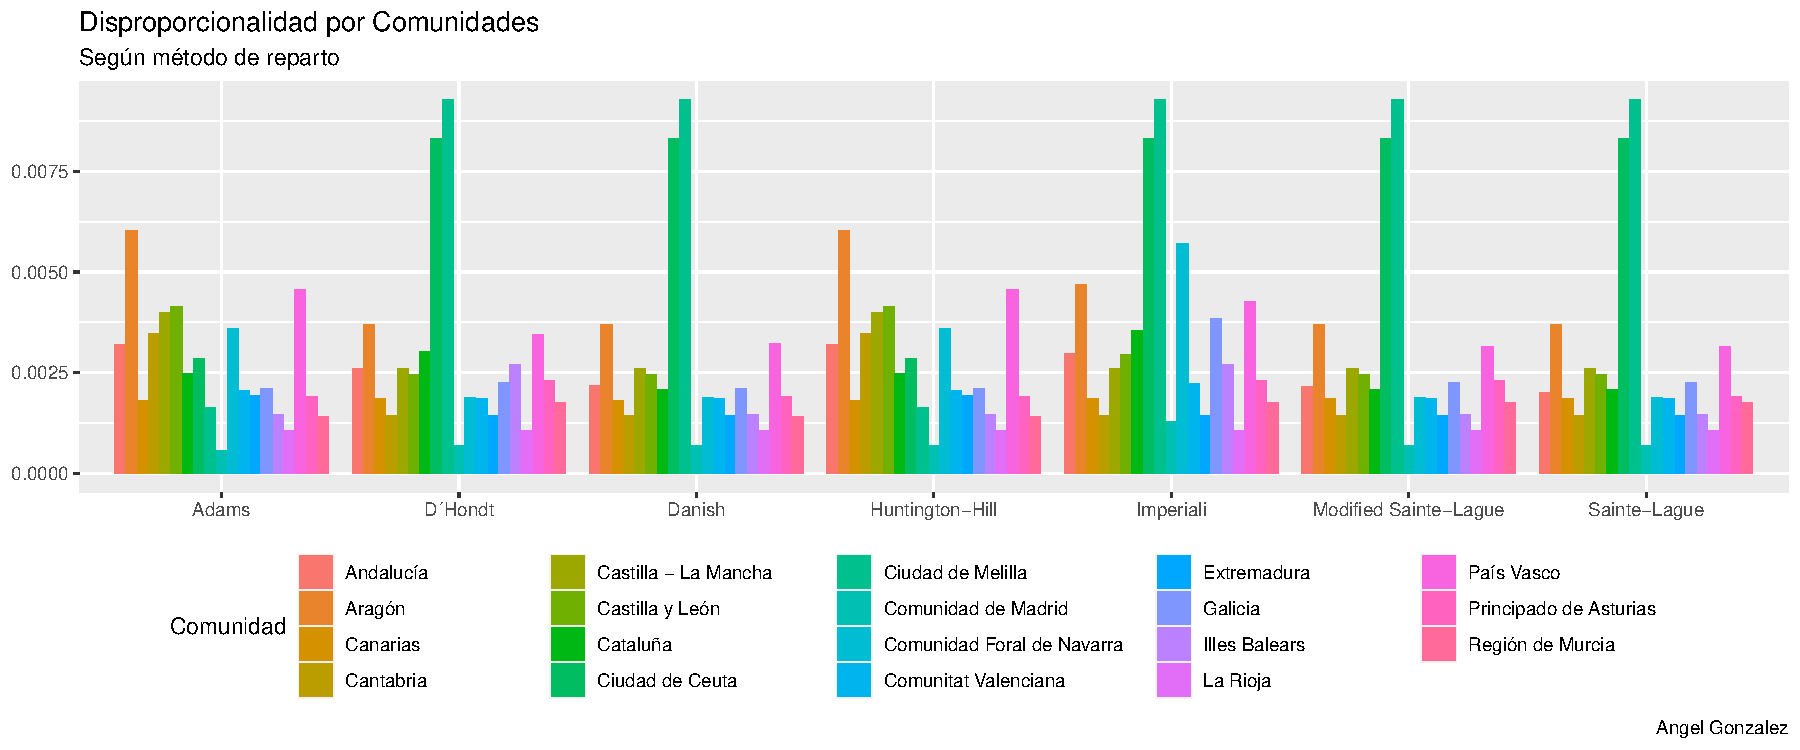
\includegraphics[width=1\linewidth]{figurasR/unnamed-chunk-84-1} \end{center}

En estas elecciones de 1982 el partido más votado es el \emph{PSOE}, el
cual según la mayoría de los métodos de reparto, incluido el método
D´Hondt, alcanza la mayoría absoluta. Son unas elecciones en los que el
voto se concentra únicamente en dos partidos, que son el \emph{PSOE} y
\emph{Alianza Popular}, pero con una gran diferencia de asientos entre
ellos, donde el \emph{PSOE} casi dobla en escaños a \emph{Alianza
Popular}. El partido menos beneficiado este año es \emph{UCD}, que según
el método D´Hondt obtendría 11 escaños mientras que si se optase por
otro método más proporcional como puede ser el método Danish o bien el
Sainte-Lague podría multiplicar sus escaños por 3 o 4.

\hypertarget{desproporciuxf3n-2}{%
\subsection{Desproporción}\label{desproporciuxf3n-2}}

\begin{center}\includegraphics[width=1\linewidth]{figurasR/unnamed-chunk-85-1} \end{center}

\begin{center}\includegraphics[width=1\linewidth]{figurasR/unnamed-chunk-85-2} \end{center}

Según la gráfica de desproporción por comunidades es un año en el que
todas ellas presentan un nivel de desproporción similar. Las comunidades
más desproporcionadas son la comunidad Foral de Navarra y Cantabria sin
contar las usuales de Ceuta y Melilla, mientras que las comunidades más
proporcionadas son la comunidad de Madrid y la región de Murcia.

Según la desproporción media, se identifican tres grupos distintos, un
grupo muy desproporcionado, con el método Imperiali como el más
desproporcionado, seguido por el Adams y Huntington-Hill. Otro grupo de
proporcionalidad media en donde se encuentra el método D´Hondt,
LR-Imperiali y Modified Sainte-Lague y un último grupo el cual sería el
más proporcionado, en el que se encuentra el método Danish, LR-Hare,
LR-Droop y el Saint-Lague.

\hypertarget{auxf1o-1986}{%
\section{Año 1986}\label{auxf1o-1986}}

\hypertarget{comparativa-de-asientos-obtenidos-3}{%
\subsection{Comparativa de asientos
obtenidos}\label{comparativa-de-asientos-obtenidos-3}}

\begin{center}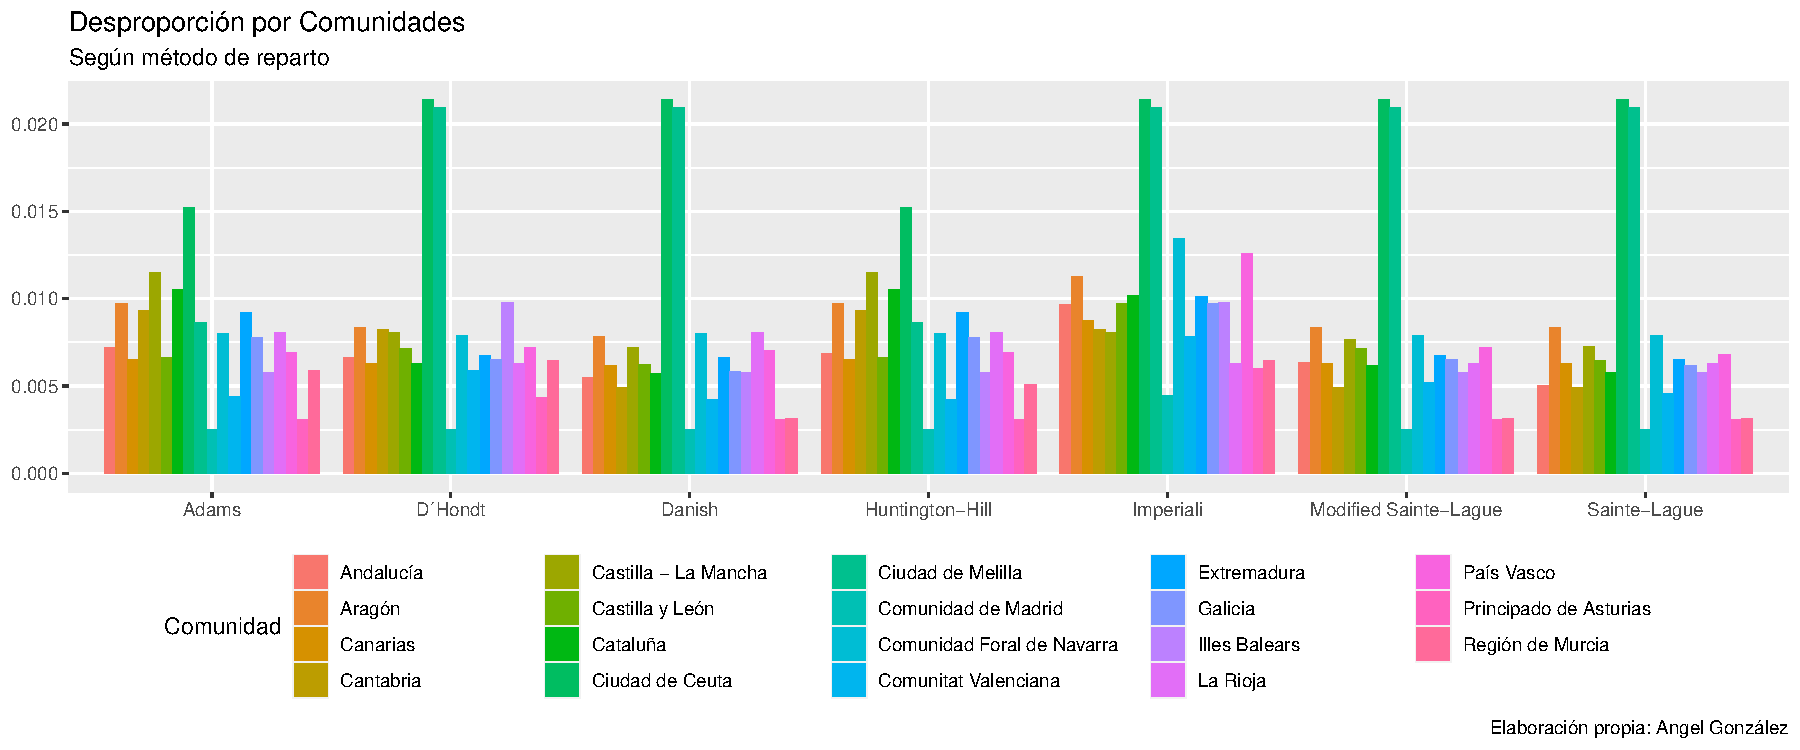
\includegraphics[width=1\linewidth]{figurasR/unnamed-chunk-87-1} \end{center}

En estas elecciones de 1986 el partido más votado fue el \emph{PSOE},
tal y como sucedió en las anteriores elecciones, son también unas
elecciones en donde hay únicamente dos partidos mayoritarios,
\emph{PSOE} y \emph{Coalición Popular}, ocurre en estas elecciones el
mismo escenario que en las anteriores elecciones, en donde el primer
partido casi dobla en escaños al segundo partido, aunque en este caso ya
se puede apreciar que la diferencia se va reduciendo entre los dos
grandes partidos, en general el PSOE alcanza la mayoría absoluta pero en
este año si utilizásemos los métodos más proporcionados es interesante
observar como perdería la mayoría absoluta tanto utilizando el método
Danish como el Sainte-Lague.\\
Este año también reconocemos un partido que podría decirse de nivel de
votos medio que queda muy dañado por el método de reparto D´Hondt, es el
partido \emph{Centro Democrático y Social}, el cual de utilizar los
métodos más proporcionales podría hasta duplicar sus escaños, por
ejemplo en el caso de optar por el método Danish.

\hypertarget{desproporciuxf3n-3}{%
\subsection{Desproporción}\label{desproporciuxf3n-3}}

\begin{center}\includegraphics[width=1\linewidth]{figurasR/unnamed-chunk-88-1} \end{center}

\begin{center}\includegraphics[width=1\linewidth]{figurasR/unnamed-chunk-88-2} \end{center}

Este año en el caso de la desproporción por comunidades podemos observar
que aumenta la diferencia respecto a las pasadas elecciones, una de las
comunidades más proporcionadas es la comunidad de Asturias mientras que
Aragón pasa a ser ahora una de las que más desproporción presenta. En
los extremos no hay novedades, Madrid sigue siendo la más proporcionada
y las ciudades de Ceuta y Melilla las que menos proporcionadas resultan.

Según el método de reparto este año el método Imperiali es el más
desproporcionado con una gran diferencia respecto a los restantes
métodos, los demás métodos se sitúan en un mismo grupo, en donde los
métodos más proporcionados este año son los métodos LR-Hare y Danish
seguido muy de cerca por el LR-Hare y el Sainte-Lague.

\hypertarget{auxf1o-1989}{%
\section{Año 1989}\label{auxf1o-1989}}

\hypertarget{comparativa-de-asientos-obtenidos-4}{%
\subsection{Comparativa de asientos
obtenidos}\label{comparativa-de-asientos-obtenidos-4}}

\begin{center}\includegraphics[width=1\linewidth]{figurasR/unnamed-chunk-90-1} \end{center}

En estas elecciones de 1989 el partido más votado es, como sucedió en
las anteriores elecciones, el \emph{PSOE}, vemos como aparece por
primera vez el \emph{Partido Popular} como segunda fuerza tomando el
puesto que antes tenía \emph{Coalición Popular}, estas elecciones
también son muy bipartidistas aunque se va debilitando ese bipartidismo,
ahora podemos decir que hay dos partidos hegemónicos, PSOE y PP, y tres
partidos medianos, los cuales serían el Centro Democrático y Social,
Izquierda Unida y Convergencia y Unión, de todos estos partidos los más
desfavorecidos por la utilización del método D´Hondt son IU y Centro
Democrático, los cuales de haber utilizado los métodos más
proporcionales podrían hasta duplicar su presencia en el congreso. Por
la otra parte en el caso del PSOE pasaría de alcanzar la mayoría
absoluta justa con 175 escaños a perder la mayoría absoluta en el caso
de optar por los métodos más proporcionales.

\hypertarget{desproporciuxf3n-4}{%
\subsection{Desproporción}\label{desproporciuxf3n-4}}

\begin{center}\includegraphics[width=1\linewidth]{figurasR/unnamed-chunk-91-1} \end{center}

\begin{center}\includegraphics[width=1\linewidth]{figurasR/unnamed-chunk-91-2} \end{center}

Este año aumenta ligeramente la diferencia de desproporción entre
comunidades, sin encontrar novedades en las comunidades más
proporcionales, Madrid, y las más desproporcionadas, las ciudades de
Ceuta y Melilla. Observando los métodos de reparto, la comunidad que
presenta especiales bajos niveles de desproporción en estas elecciones
es la región de Murcia.

Estas elecciones de 1989 la desproporción media se agrupa en tres
grupos, de alta, media y baja desproporción, el más desproporcionado
vuelve a ser el método Imperiali, el método D´Hondt sigue siendo el más
desproporcionado en el grupo medio y el método más proporcionado vuelve
a ser el Danish aunque le sigue muy cerca el método Sainte-Lague.

\hypertarget{auxf1o-1993}{%
\section{Año 1993}\label{auxf1o-1993}}

\hypertarget{comparativa-de-asientos-obtenidos-5}{%
\subsection{Comparativa de asientos
obtenidos}\label{comparativa-de-asientos-obtenidos-5}}

\begin{center}\includegraphics[width=1\linewidth]{figurasR/unnamed-chunk-93-1} \end{center}

En las elecciones de 1993 podemos observar como la fuerza del primer
partido va decreciendo lentamente. Los dos partidos más votados son el
\emph{PSOE} y el \emph{PP} respectivamente. La diferencia de estas
elecciones respecto a las anteriores es que el PSOE ha perdido la
mayoría absoluta según el método D´Hondt y en cambio el \emph{PP} ha
aumentado su presencia significativamente, y está ya relativamente cerca
de alcanzar al \emph{PSOE}. De haber utilizado los métodos más
proporcionales resultaría en una menor diferencia de escaños entre estos
dos grandes partidos, el partido más castigado en estas elecciones sigue
siendo \emph{IU}, el cual podría haber obtenido de 1.5 a 2 veces más
asientos de haber cambiado de método de reparto. Son unas elecciones en
donde hay dos partidos hegemónicos y dos partidos medianos, que son
\emph{IU} y \emph{CIU}, como hemos visto \emph{IU} es un partido muy
castigado por el método de reparto actual, en cambio \emph{CIU} no se
vería agraviado o beneficiado al cambiar el método de reparto.

\hypertarget{desproporciuxf3n-5}{%
\subsection{Desproporción}\label{desproporciuxf3n-5}}

\begin{center}\includegraphics[width=1\linewidth]{figurasR/unnamed-chunk-94-1} \end{center}

\begin{center}\includegraphics[width=1\linewidth]{figurasR/unnamed-chunk-94-2} \end{center}

En estas elecciones se observan más picos de desproporción en
comparación con las elecciones anteriores, especialmente aumenta su
desproporción el Pais Vasco y Cantabria, no hay novedades en los máximos
ni en los mínimos. Siguen dos grupos con un comportamiento similar, en
un grupo los métodos de Adams, Huntington-Hill y LR-Imperiali y los
restantes en el otro grupo.

Este año en el caso de la desproporción media según el método de reparto
vemos que hay diferencias en los métodos más desproporcionales,
usualmente el método más desproporcionado ha sido el Imperiali, en estas
elecciones esto cambia, de hecho mejora en dos puestos. Los más
desproporcionados este año entonces son los métodos Adams y de
Huntington-Hill, en el caso de los más proporcionados se encuentran los
métodos LR-Imperiali, LR-Hare y Danish seguido muy de cerca por el
Sainte-Lague.

\hypertarget{auxf1o-1996}{%
\section{Año 1996}\label{auxf1o-1996}}

\hypertarget{comparativa-de-asientos-obtenidos-6}{%
\subsection{Comparativa de asientos
obtenidos}\label{comparativa-de-asientos-obtenidos-6}}

\begin{center}\includegraphics[width=1\linewidth]{figurasR/unnamed-chunk-96-1} \end{center}

En estas elecciones de 1996 son las primeras elecciones en donde el
\emph{PP} es la fuerza más votada, el \emph{PSOE} que ya llevaba una
tendencia descendiente a lo largo de las últimas elecciones al final
pierde el primer puesto a favor del \emph{PP}. Sigue presentándose un
bipartidismo significativo, seguidamente de dos partidos medianos,
todavía el PP a pesar de ganar las elecciones no alcanza la mayoría
absoluta en ninguno de los métodos analizados. Izquierda Unida sigue
siendo el partido más castigado, podría duplicar el número de escaños de
haber escogido otro método más proporcional.

\hypertarget{desproporciuxf3n-6}{%
\subsection{Desproporción}\label{desproporciuxf3n-6}}

\begin{center}\includegraphics[width=1\linewidth]{figurasR/unnamed-chunk-97-1} \end{center}

\begin{center}\includegraphics[width=1\linewidth]{figurasR/unnamed-chunk-97-2} \end{center}

En estas elecciones de 1996 se observa una desproporción similar a las
elecciones anteriores, en este año el comportamiento de la desproporción
por provincias se puede agrupar en tres grupos, uno en el que estaría el
método LR-Imperiali, con una desproporción alta en la comunidad Foral de
Navarra, otro en los que estarían los métodos Adams y Huntington-Hill,
con una alta desproporción en la Rioja y un tercer grupo con los
restantes métodos.

Este año en el caso de la desproporción media según el método de reparto
vemos que hay diferencias en los métodos con más desproporción respecto
a la anterior elección, el método más desproporcionado vuelve a ser el
Imperiali. En el caso de los más proporcionados cambia también, el
método Danish pasa a un cuarto puesto superado por el método
Sainte-Lague, los mejores son el método LR-Imperiali y LR-Hare. Los más
desproporcionados este año son el método anteriormente citado,
Imperiali, seguido muy de cerca por los métodos Adams y de
Huntington-Hill.

\hypertarget{auxf1o-2000}{%
\section{Año 2000}\label{auxf1o-2000}}

\hypertarget{comparativa-de-asientos-obtenidos-7}{%
\subsection{Comparativa de asientos
obtenidos}\label{comparativa-de-asientos-obtenidos-7}}

\begin{center}\includegraphics[width=1\linewidth]{figurasR/unnamed-chunk-99-1} \end{center}

En las elecciones del año 2000 el partido más votado vuelve a ser el
\emph{Partido Popular} seguido del \emph{PSOE}. En estas elecciones,
según el método D´Hondt utilizado en España el \emph{PP} conseguiría una
mayoría absoluta holgada, es una elección con un claro bipartidismo
donde se podría decir que no existen partidos medianos. Si optásemos por
otro método de reparto más proporcional como puede ser el método Danish
o el Sainte-Lague el PP alcanzaría la mayoría absoluta o se quedaría a
muy pocos escaños de alcanzarla, en cambio veríamos a muchos partidos
pequeños con menos de tres votos casi duplicar su presencia en escaños.
El partido más castigado por utilizar el método D´Hondt en estas
elecciones sigue siendo Izquierda Unida.

\hypertarget{desproporciuxf3n-7}{%
\subsection{Desproporción}\label{desproporciuxf3n-7}}

\begin{center}\includegraphics[width=1\linewidth]{figurasR/unnamed-chunk-100-1} \end{center}

\begin{center}\includegraphics[width=1\linewidth]{figurasR/unnamed-chunk-100-2} \end{center}

Observando la desproporción por comunidades tanto el método Adams como
el Huntington-Hill tienen un comportamiento diferente respecto a los
demás, siguen siendo los más desproporcionados las ciudades de Ceuta y
Melilla, y la más proporcionada la Comunidad de Madrid, este año es
especialmente alta la desproporción de las Islas Baleares respecto a
anteriores elecciones.

Si miramos la gráfica de la desproporción según el método de reparto se
pueden agrupar los métodos en dos grupos, uno con gran desproporción en
el que estarían incluidos los métodos Adams, Huntington-Hill e Imperiali
respectivamente, y el otro grupo restante con una desproporción entre
media y baja. Seguimos observando que el método D´Hont sigue en las
peores posiciones dentro del grupo con desproporción media y baja,
siendo los mejores el método LR-Hare, Danish y Saint-Lague, todos ellos
con una desproporción muy similar.

\hypertarget{auxf1o-2004}{%
\section{Año 2004}\label{auxf1o-2004}}

\hypertarget{comparativa-de-asientos-obtenidos-8}{%
\subsection{Comparativa de asientos
obtenidos}\label{comparativa-de-asientos-obtenidos-8}}

\begin{center}\includegraphics[width=1\linewidth]{figurasR/unnamed-chunk-102-1} \end{center}

En estas elecciones del año 2004 volvemos a ver unas elecciones con un
claro bipartidismo y con una diferencia de escaños entre partidos cada
vez menor, en estas elecciones el partido más votado cambia y el
\emph{PSOE} obtiene los mayores votos, seguido del \emph{PP} que pierde
la mayoría absoluta según D´Hont que tenía en las anteriores elecciones.
En ningún método el \emph{PSOE} alcanzaría la mayoría absoluta por lo
que deberá de realizar alianzas con otros partidos para así alcanzar la
mayoría absoluta. En el caso de optar por los métodos más proporcionales
resultaría en una reducción muy significativa de la diferencia de
escaños entre partidos que pasaría de una diferencia de 16 escaños a 6
escaños en el caso de optar por el método Danish. El partido más
castigado por el método D´Hondt es \emph{Izquierda Unida}, que hasta
podría ver duplicado o triplicado su presencia en el congreso si se opta
por utilizar un método de reparto más proporcional.

\hypertarget{desproporciuxf3n-8}{%
\subsection{Desproporción}\label{desproporciuxf3n-8}}

\begin{center}\includegraphics[width=1\linewidth]{figurasR/unnamed-chunk-103-1} \end{center}

\begin{center}\includegraphics[width=1\linewidth]{figurasR/unnamed-chunk-103-2} \end{center}

Según el gráfico por comunidades se sigue la tónica general de las
anteriores elecciones, únicamente podemos apreciar en estas elecciones
una reducción de la desproporción entre comunidades, es decir, una menor
diferencia de desproporción entre ellas. Siguen dos grupos con
comportamiento similar, un grupo donde se encuentran los métodos Adams,
Huntington-Hill y LR-Imperiali, y en otro grupo los restantes. En el
caso de agrupar la desproporción por métodos observamos que este año el
método más desproporcionado es el Huntington-Hill, mientras que en la
parte de los métodos más proporcionados el método mejor sería el
LR-Imperiali, LR-Hare y Sainte-Lague. El método D´Hondt utilizado en
España sigue siendo un método que se encuentra en un nivel medio, sin
destacar por una desproporción alta ni baja entre todos los métodos.

\hypertarget{auxf1o-2008}{%
\section{Año 2008}\label{auxf1o-2008}}

\hypertarget{comparativa-de-asientos-obtenidos-9}{%
\subsection{Comparativa de asientos
obtenidos}\label{comparativa-de-asientos-obtenidos-9}}

\begin{center}\includegraphics[width=1\linewidth]{figurasR/unnamed-chunk-105-1} \end{center}

En estos comicios del año 2008 no hay diferencias significativas en
términos de escaños, sigue un claro bipartidismo con dos partidos
hegemónicos, en primer lugar el más votado en estas elecciones que sigue
siendo el \emph{PSOE} seguido por el \emph{PP}, la diferencia de escaños
entre ellos continúa siendo prácticamente la misma pero en este año el
bipartidismo es cada vez más pronunciado, aumentando ambos partidos su
presencia en el congreso. Para el partido más votado únicamente en dos
casos podría obtener la mayoría absoluta, que sería en el caso de optar
por el método Imperiali, una mayoría absoluta justa al llegar sólo a los
175 escaños o bien por el método LR-Imperiali que alcanzaría los 180
escaños. Utilizando los métodos de reparto más proporcionales como son
el Danish y el Sainte-Lague la diferencia entre los partidos más votados
se reduciría a la vez que obtendrían un menor número de escaños, el
partido más perjudicado sigue siendo Izquierda Unida que podría hasta
más que quintuplicar su presencia en el congreso de haber optado por el
método Danish.

\hypertarget{desproporciuxf3n-9}{%
\subsection{Desproporción}\label{desproporciuxf3n-9}}

\begin{center}\includegraphics[width=1\linewidth]{figurasR/unnamed-chunk-106-1} \end{center}

\begin{center}\includegraphics[width=1\linewidth]{figurasR/unnamed-chunk-106-2} \end{center}

Este es un año en el que se puede observar una mayor igualdad en el caso
de las desproporciones, las comunidades no tienen una gran diferencia de
proporcionalidad entre ellas sin contar con las habituales de Ceuta y
Melilla, además no encontramos grandes diferencias entre los métodos.\\
Si observamos la gráfica de la desproporción según el método de reparto,
el método más despropocionado es el Imperiali, seguido por los métodos
Adams y Huntington-Hill. Todos los demás métodos están en un mismo
nivel, el mejor método en estas elecciones es el método LR-Imperiali,
que presenta una muy baja desproporción respecto a los demás métodos. El
método D´Hont utilizado en España no presenta diferencias y se encuentra
en un nivel medio-alto de desproporción entre todos los métodos
analizados.

\hypertarget{auxf1o-2011}{%
\section{Año 2011}\label{auxf1o-2011}}

\hypertarget{comparativa-de-asientos-obtenidos-10}{%
\subsection{Comparativa de asientos
obtenidos}\label{comparativa-de-asientos-obtenidos-10}}

\begin{center}\includegraphics[width=1\linewidth]{figurasR/unnamed-chunk-108-1} \end{center}

Este año 2011 podemos considerarlo como el primer año en el que aunque
continúe sucediendo un claro bipartidismo empiezan a surgir partidos
medianos con cada vez más presencia en el congreso, en este año es la
aparición de \emph{UPyD}. El partido más votado en estas elecciones es
el \emph{Partido Popular}, que además obtiene la mayoría absoluta de
forma holgada según el método D´Hondt utilizado en España, le sigue el
\emph{PSOE} a una diferencia muy significativa, casi duplica la
presencia en el congreso del \emph{PP} respecto al \emph{PSOE}. Si
observamos los otros métodos propuestos vemos que el \emph{PP} en el
caso del método Danish no llegaría a obtener la mayoría absoluta pero si
utilizásemos el método de Sainte-Lague sí que alcanzaríamos la mayoría
absoluta con 176 escaños. Los partidos más perjudicados por utilizar el
método D´Hont son en estas elecciones \emph{UPyD} y \emph{IU}, los
cuales de haber optado por el método Danish podrían duplicar su
presencia en el congreso. Es llamativo el resultado de las elecciones
según el método Adams y Huntington-Hill, son métodos que dan escaños a
los partidos con menos votos en detrimento de los partidos más votados,
en estas elecciones vemos como el resultado cambiaría radicalmente, el
\emph{PP} de ser el partido más votado con mucha diferencia pasaría a
reducir la diferencia de escaños respecto al \emph{PSOE} a la mitad
según el método Adams, pero la diferencia más notoria está en los
partidos medianos \emph{UPyD} y \emph{IU}, que pasarían de 5 a 30
escaños y de 11 a 43 escaños respectivamente.

\hypertarget{desproporciuxf3n-10}{%
\subsection{Desproporción}\label{desproporciuxf3n-10}}

\begin{center}\includegraphics[width=1\linewidth]{figurasR/unnamed-chunk-109-1} \end{center}

\begin{center}\includegraphics[width=1\linewidth]{figurasR/unnamed-chunk-109-2} \end{center}

Observando el gráfico de la desproporción entre comunidades vemos como
este año se aprecian claramente dos grupos distintos. Uno en el que se
encuentran niveles similares de desproporción entre las comunidades y
otro grupo en el que se encuentran los métodos Imperiali, Adams y
Huntington-Hill, con grandes diferencias de desproporción entre
comunidades.

En la desproporción media según el método de reparto volvemos a observar
dos grupos bien diferenciados, uno en el que hay una gran desproporción,
donde estarían los métodos Huntington-Hill, Adams e Imperiali, y otro
grupo con los restantes métodos con una proporcionalidad baja. El método
D´Hondt utilizado en España se encontraría en el grupo de desproporción
media, pero dentro del grupo es el más desproporcionado. Los mejores
métodos en estas elecciones son el método LR-Hare y Danish.

\hypertarget{auxf1o-2015}{%
\section{Año 2015}\label{auxf1o-2015}}

\hypertarget{comparativa-de-asientos-obtenidos-11}{%
\subsection{Comparativa de asientos
obtenidos}\label{comparativa-de-asientos-obtenidos-11}}

\begin{center}\includegraphics[width=1\linewidth]{figurasR/unnamed-chunk-111-1} \end{center}

En estas elecciones del 2015 observamos que el bipartidismo que veíamos
omnipresente en todas las elecciones anteriores ahora ya no ocurre, es
el primer año en el que se puede afirmar que ya no hay un bipartidismo
claro. El partido más votado es el \emph{Partido Popular} seguido por el
\emph{PSOE}, pero ya vemos que este año aparecen dos nuevos partidos
medianos, que son \emph{Podemos} y \emph{Ciudadanos.} El partido más
votado no obtiene la mayoría absoluta en ningún método. Es interesante
observar como entre \emph{Podemos} y \emph{Ciudadanos} en el caso de
utilizar el método D´Hondt, el primero superaría en dos escaños al
segundo, mientras que de haber utilizado el método Danish,
\emph{Ciudadanos} superaría a \emph{Podemos} en dos escaños. En el caso
de optar por el método Danish, el partido más votado, el \emph{PP},
perdería bastantes escaños y su diferencia respecto al segundo se vería
reducida significativamente. En el caso de los partidos medianos verían
aumentar levemente su presencia en el congreso pero en ningún caso
supondría un cambio significativo. El partido más perjudicado este año
vuelve a ser \emph{Izquierda Unida}, que podría pasar de obtener 2
escaños con el método D´Hondt a 11 escaños con el Danish.

\hypertarget{desproporciuxf3n-11}{%
\subsection{Desproporción}\label{desproporciuxf3n-11}}

\begin{center}\includegraphics[width=1\linewidth]{figurasR/unnamed-chunk-112-1} \end{center}

\begin{center}\includegraphics[width=1\linewidth]{figurasR/unnamed-chunk-112-2} \end{center}

Según el gráfico por comunidades volvemos a ver un comportamiento
similar entre los distintos métodos, con pequeñas diferencias en el
grupo de los métodos Imperiali, Adams y Huntington-Hill. Es un año en el
que la diferencia de desproporción entre las distintas comunidades
aumentan. Siguen presentándose las mayores desproporciones en Ceuta y
Melilla y la menor desproporción en la comunidad de Madrid.

En el caso de la desproporción según el método de reparto este año
tenemos nuevamente dos grupos diferenciados, un grupo con una
desproporción alta en el que se encontraría el método Imperiali,
Huntington-Hill y Adams, respectivamente, y todos los métodos restantes
se encontrarían en el grupo de desproporción media o baja, el mejor
método este año es el LR-Hare y el Sainte-Lague, encontramos que el
método D´Hondt utilizado en España es el peor método posible dentro del
grupo con baja desproporción, por lo tanto sería conveniente plantear el
cambio a otro método mejor.

\hypertarget{auxf1o-2016}{%
\section{Año 2016}\label{auxf1o-2016}}

\hypertarget{comparativa-de-asientos-obtenidos-12}{%
\subsection{Comparativa de asientos
obtenidos}\label{comparativa-de-asientos-obtenidos-12}}

\begin{center}\includegraphics[width=1\linewidth]{figurasR/unnamed-chunk-114-1} \end{center}

En las elecciones del año 2016 vemos como se va consolidando el modelo
de las anteriores elecciones, con dos grandes partidos y dos partidos
medianos. La fuerza política más votada este año es el \emph{Partido
Popular} seguido del \emph{PSOE}, en ningún método el \emph{PP}
alcanzaría la mayoría absoluta. Son unas elecciones que presentan
similares resultados sea cual sea el método de reparto, en el caso de
utilizar el método Danish respecto al D´Hondt resultaría en un menor
número de escaños para el \emph{PP} y una ligera subida de escaños de
\emph{Podemos} y \emph{Ciudadanos}.

Son las primeras elecciones en donde el método de reparto no cambia
significativamente el reparto de escaños, es notorio que en este año el
\emph{PSOE} obtenga casi los mismos escaños independientemente del
método de reparto utilizado.

\hypertarget{desproporciuxf3n-12}{%
\subsection{Desproporción}\label{desproporciuxf3n-12}}

\begin{center}\includegraphics[width=1\linewidth]{figurasR/unnamed-chunk-115-1} \end{center}

\begin{center}\includegraphics[width=1\linewidth]{figurasR/unnamed-chunk-115-2} \end{center}

En la desproporción por comunidades vemos un comportamiento similar
entre los distintos métodos, únicamente el método Imperiali tiene un
comportamiento levemente diferente a los demás. Este año es
especialmente alta la desproporción de la ciudad de Ceuta y
especialmente baja la desproporción del principado de Asturias.

En el gráfico en que comparamos los métodos de reparto el comportamiento
es similar al anterior año, con un método que es significativamente
desproporcionado respecto a los demás, el método Imperiali, y los demás
métodos similares entre ellos, siendo el mejor método el LR-Hare y
Sainte-Lague. El método utilizado en España, el D´Hondt, vuelve a ser de
los peores, por lo que sería necesario proponer un cambio de método de
reparto a otro más proporcional.

\hypertarget{auxf1o-2019-abril}{%
\section{Año 2019, Abril}\label{auxf1o-2019-abril}}

\hypertarget{comparativa-de-asientos-obtenidos-13}{%
\subsection{Comparativa de asientos
obtenidos}\label{comparativa-de-asientos-obtenidos-13}}

\begin{center}\includegraphics[width=1\linewidth]{figurasR/unnamed-chunk-117-1} \end{center}

En estas elecciones de Abril de 2019 vemos como ya no existe el
bipartidismo, este año podemos agrupar a los partidos políticos en
cuatro categorías, la primera en donde hay un partido con muchos votos
con una gran diferencia de escaños respecto a los demás, que es el
\emph{PSOE}, un segundo grupo en donde se encontrarían dos partidos con
un número medio-alto de escaños, que son el \emph{PP} y
\emph{Ciudadanos} respectivamente, un tercer grupo con un número mediano
de escaños con \emph{Podemos} y \emph{Vox}, y un último grupo de pocos
escaños con los demás partidos. Este año tampoco hay diferencias de
escaños de haber utilizado un método de reparto respecto a otro, los
partidos más perjudicados por la elección del método D´Hondt son
\emph{Vox} y \emph{Podemos}, en ningún caso el partido más votado
alcanza la mayoría absoluta. De haber utilizado el método Danish el
partido que se vería más beneficiado sería \emph{Vox} seguido de
\emph{Ciudadanos}, partido que superaría en escaños al \emph{PP} y se
convertiría en la segunda fuerza en el hemiciclo, igualmente sucedería
con los métodos Adams y Huntington-Hill.

\hypertarget{desproporciuxf3n-13}{%
\subsection{Desproporción}\label{desproporciuxf3n-13}}

\begin{center}\includegraphics[width=1\linewidth]{figurasR/unnamed-chunk-118-1} \end{center}

\begin{center}\includegraphics[width=1\linewidth]{figurasR/unnamed-chunk-118-2} \end{center}

Este es un año en el que viendo la desproporción por comunidades es
especialmente similar independientemente del método utilizado. En las
ciudades de Ceuta y Melilla es donde encontramos la mayor desproporción,
por otra parte la comunidad de Madrid es la provincia más
proporcionada.\\
Cuando comparamos la proporcionalidad según el método de reparto sucede
algo similar a las anteriores elecciones, en donde el método Imperiali
se encuentra con una diferencia bastante significativa respecto a las
demás. El método utilizado en España vuelve a ser uno de los peores, en
estas elecciones baja hasta ser el segundo peor en términos de
proporcionalidad, es un método que no está preparado para ser óptimo en
escenarios en donde no hay un bipartidismo claro.

\hypertarget{auxf1o-2019-noviembre}{%
\section{Año 2019, Noviembre}\label{auxf1o-2019-noviembre}}

\hypertarget{comparativa-de-asientos-obtenidos-14}{%
\subsection{Comparativa de asientos
obtenidos}\label{comparativa-de-asientos-obtenidos-14}}

\begin{center}\includegraphics[width=1\linewidth]{figurasR/unnamed-chunk-120-1} \end{center}

En esta gráfica de las elecciones de Noviembre de 2019 podemos observar
una ligera recuperación del bipartidismo en donde los dos principales
partidos vuelven a aumentar el número de escaños obtenidos y también
aumentar la diferencia en escaños respecto a los demás.\\
Son unas elecciones en donde hay dos partidos principales, que son el
\emph{PSOE} y el \emph{PP} respectivamente, uno medio en escaños,
\emph{Vox}, y tres partidos de un nivel medio-bajo de escaños, que son
\emph{Podemos}, \emph{ERC} y \emph{Ciudadanos} respectivamente.\\
En el caso de optar por otro método de reparto de escaños no se
alcanzaría la mayoría absoluta en ninguno de ellos. Hay dos partidos
perjudicados por utilizar el método D´Hondt en vez de otro más
proporcional como pueda ser el Danish, son los partidos de
\emph{Podemos} que pasarían de obtener 26 escaños a 40 y el partido
\emph{Ciudadanos} que pasaría a duplicar su presencia de 10 escaños a
23.

\hypertarget{desproporciuxf3n-14}{%
\subsection{Desproporción}\label{desproporciuxf3n-14}}

\begin{center}\includegraphics[width=1\linewidth]{figurasR/unnamed-chunk-121-1} \end{center}

\begin{center}\includegraphics[width=1\linewidth]{figurasR/unnamed-chunk-121-2} \end{center}

En el gráfico por comunidades obtenemos el mismo comportamiento que en
las elecciones anteriores sin observar diferencias notables. Siguen
siendo Ceuta y Melilla las regiones mas desproporcionadas y Madrid la
más proporcionada.\\
Cuando comparamos la desproporción según el método de reparto, el método
Imperiali sigue siendo el más desproporcionado mientras que el mejor
método esta vez resulta ser el LR-Hare y Sainte-Lague, el método D´Hondt
como hemos visto en la anterior elección sigue siendo el segundo peor
método posible entre todos los analizados.

\hypertarget{comparativa-entre-auxf1os}{%
\section{Comparativa entre años}\label{comparativa-entre-auxf1os}}

En este apartado final procederemos a agrupar todos los resultados de la
desproporción, los agruparemos por año y método. Con todo ello
realizaremos dos gráficos, uno en el que muestre la desproporción a lo
largo de los años distinguiendo el método de reparto utilizado y otro en
el que muestre el promedio de la desproporción a lo largo de todos los
años analizados para cada método.

\begin{center}\includegraphics[width=1\linewidth]{figurasR/unnamed-chunk-122-1} \end{center}

En este gráfico comparando la desproporción media por año observamos
como la desproporción desde las elecciones de 1977 hasta 1989 está en un
nivel medio o alto. A partir del año 1993 la desproporción es baja,
principalmente debido a un bipartidismo más marcado, esto se mantiene
hasta el año de las elecciones de 2011, en donde empieza por primera vez
a aparecer un tercer partido que debilita el bipartidismo, por lo que la
desproporción aumenta a los niveles de las primeras elecciones de 1977,
desde el año 2011 hasta las últimas elecciones de 2019 la desproporción
se mantiene sin mucha variación.

\begin{center}\includegraphics[width=1\linewidth]{figurasR/unnamed-chunk-123-1} \end{center}

En el gráfico de la desproporción según el método de reparto podemos
extraer conclusiones para decidir qué método ha sido el mejor a lo largo
de todas las elecciones realizadas en España a partir de 1977, por lo
tanto sacamos estas conclusiones:

\begin{itemize}
\tightlist
\item
  El mejor método es el Saint-Lague por parte de los métodos de promedio
  mayor y por los métodos de resto mayor el mejor método es el LR-Hare,
  que también es el mejor método entre todos los analizados.
\item
  El peor método entre todos los analizados es el método Imperiali.
\item
  El método utilizado en España, el método D´Hondt, es el séptimo mejor
  método en términos de proporcionalidad o bien el cuarto peor método.
\end{itemize}

Por lo tanto al preguntarnos si el método utilizado en España, método
D´Hont, es el mejor método de reparto de escaños en términos de
desproporción, podemos afirmar que no lo es, de hecho se sitúa en la
mitad alta de la tabla entre todos los métodos analizados. La
característica que tiene el método D´Hont es que se sitúa entre los
métodos que benefician más a los partidos más votados y de entre ellos
es el método más proporcional, por lo que se podría decir que es el
método más proporcional entre los métodos que ``facilitan la
gobernanza''. Si nuestro objetivo es obtener la máxima proporcionalidad
en vez de facilitar la gobernanza, deberíamos plantear un cambio de
método, en primer lugar al Sainte-Lague o al Danish en el caso de los
métodos de promedio mayor, ambos métodos son casi idénticos en términos
de proporcionalidad pero el Sainte-Lague tiene una mejor característica
que el Danish, que reparte los escaños de forma que es más fácil
gobernar, o bien al método LR-Hare en el caso de los métodos de resto
mayor. En cambio si queremos facilitar la gobernanza a la vez que
tratamos de minimizar la desproporción entre los escaños y los votos, en
este caso el método D´Hondt es donde muestra su valor, puesto que es
como hemos comentado anteriormente, el método que entra dentro del grupo
que benefician más a los partidos más votados y de entre ellos es el
método más proporcional, por esta razón se puede considerar el método
más equilibrado para el gobierno de una nación.

\FloatBarrier

\ifdefined\ifprincipal
\else
\setlength{\parindent}{1em}
\pagestyle{fancy}
\setcounter{tocdepth}{4}
\tableofcontents

\fi

\ifdefined\ifdoblecara
\fancyhead{}{}
\fancyhead[LE,RO]{\scriptsize\rightmark}
\fancyfoot[LO,RE]{\scriptsize\slshape \leftmark}
\fancyfoot[C]{}
\fancyfoot[LE,RO]{\footnotesize\thepage}
\else
\fancyhead{}{}
\fancyhead[RO]{\scriptsize\rightmark}
\fancyfoot[LO]{\scriptsize\slshape \leftmark}
\fancyfoot[C]{}
\fancyfoot[RO]{\footnotesize\thepage}
\fi
\renewcommand{\headrulewidth}{0.4pt}
\renewcommand{\footrulewidth}{0.4pt}

\hypertarget{influencia-de-las-delimitaciones-de-las-circunscripciones}{%
\chapter{Influencia de las delimitaciones de las
circunscripciones}\label{influencia-de-las-delimitaciones-de-las-circunscripciones}}

En este apartado procederemos a analizar la influencia en la
proporcionalidad escaños-votos que resulta de repartir los escaños en un
distrito único, España, y el reparto actual de votos que se realiza por
provincias.\\
Procederemos de la siguiente forma:

\begin{itemize}
\item
  Con los datos obtenidos en el capítulo 4, crearemos para cada año una
  tabla con los votos resultantes de que los escaños se repartan en un
  único distrito.
\item
  Crearemos dos funciones adicionales para calcular tanto los escaños
  obtenidos como la desproporción.

  \begin{itemize}
  \item
    Función sindelim0: Aplica el método D`Hondt para España como
    distrito único, en esta función no hay un mínimo de porcentaje para
    poder ser elegido.
  \item
    Función sindelim3: Aplica el método D`Hondt para España como
    distrito único, pero con un porcentaje mínimo del 3\% para poder ser
    elegido.
  \end{itemize}
\item
  Una vez obtenidos los escaños correspondientes los comparamos con el
  método D`Hondt utilizado actualmente en España. Para evitar que sea
  muy extenso el análisis de todas las elecciones nos centraremos en
  tres de ellas, los resultados de las restantes elecciones se pueden
  encontrar en el Anexo 2.
\item
  Para analizar la desproporción agruparemos los resultados de todos los
  métodos analizados anteriormente en el capítulo 4 y los compararemos.
\end{itemize}

\newpage

\hypertarget{escauxf1os}{%
\section{Escaños}\label{escauxf1os}}

\begin{table}

\caption{\label{tab:unnamed-chunk-130}Año 1977}
\centering
\resizebox{\linewidth}{!}{
\begin{tabular}[t]{llll}
\toprule
\multicolumn{1}{c}{\textbf{}} & \multicolumn{3}{c}{\textbf{Métodos}} \\
\cmidrule(l{3pt}r{3pt}){2-4}
Partidos & DHondt & SinDelim & SinDelim3\\
\midrule
\cellcolor{gray!6}{\textcolor{blue}{\em{\textbf{UNION DE CENTRO DEMOCRATICO}}}} & \cellcolor{gray!6}{\textcolor[HTML]{DEE318}{\textbf{165}}} & \cellcolor{gray!6}{\textcolor[HTML]{DEE318}{\textbf{128}}} & \cellcolor{gray!6}{\textcolor[HTML]{DEE318}{\textbf{141}}}\\
\textcolor{blue}{\em{\textbf{PARTIDO SOCIALISTA OBRERO ESPAÑOL}}} & \textcolor[HTML]{3ABA76}{\textbf{118}} & \textcolor[HTML]{7FD34E}{\textbf{109}} & \textcolor[HTML]{7FD34E}{\textbf{120}}\\
\cellcolor{gray!6}{\textcolor{blue}{\em{\textbf{PARTIDO COMUNISTA DE ESPAÑA}}}} & \cellcolor{gray!6}{\textcolor[HTML]{48297A}{\textbf{20}}} & \cellcolor{gray!6}{\textcolor[HTML]{3A538B}{\textbf{34}}} & \cellcolor{gray!6}{\textcolor[HTML]{3A548C}{\textbf{38}}}\\
\textcolor{blue}{\em{\textbf{FEDERACION DE PARTIDOS DE ALIANZA POPULAR}}} & \textcolor[HTML]{482374}{\textbf{16}} & \textcolor[HTML]{3E4A89}{\textbf{30}} & \textcolor[HTML]{3E4A89}{\textbf{33}}\\
\cellcolor{gray!6}{\textcolor{blue}{\em{\textbf{PARTIDO SOCIALISTA POPULAR - UNIDAD SOCIALISTA}}}} & \cellcolor{gray!6}{\textcolor[HTML]{470E61}{\textbf{6}}} & \cellcolor{gray!6}{\textcolor[HTML]{472B7A}{\textbf{16}}} & \cellcolor{gray!6}{\textcolor[HTML]{472C7A}{\textbf{18}}}\\
\addlinespace
\textcolor{blue}{\em{\textbf{COALICION ELECT.PACTE DEMOCRATIC PER CATALUNYA}}} & \textcolor[HTML]{48186A}{\textbf{11}} & \textcolor[HTML]{481C6E}{\textbf{10}} & \textcolor[HTML]{440154}{\textbf{0}}\\
\cellcolor{gray!6}{\textcolor{blue}{\em{\textbf{EUZKO ALDERDI JELTZALEA-PARTIDO NACIONALISTA VASCO}}}} & \cellcolor{gray!6}{\textcolor[HTML]{471264}{\textbf{8}}} & \cellcolor{gray!6}{\textcolor[HTML]{471264}{\textbf{6}}} & \cellcolor{gray!6}{\textcolor[HTML]{440154}{\textbf{0}}}\\
\textcolor{blue}{\em{\textbf{COALICION ELECT. EQUIPO DE LA DEMOCRACIA CRISTIANA}}} & \textcolor[HTML]{440154}{\textbf{0}} & \textcolor[HTML]{470C5F}{\textbf{4}} & \textcolor[HTML]{440154}{\textbf{0}}\\
\cellcolor{gray!6}{\textcolor{blue}{\em{\textbf{UNIO DEL CENTRE I LA DEM. CRISTIANA DE CATALUNYA}}}} & \cellcolor{gray!6}{\textcolor[HTML]{450559}{\textbf{2}}} & \cellcolor{gray!6}{\textcolor[HTML]{46095D}{\textbf{3}}} & \cellcolor{gray!6}{\textcolor[HTML]{440154}{\textbf{0}}}\\
\textcolor{blue}{\em{\textbf{ALIANZA SOCIALISTA DEMOCRATICA}}} & \textcolor[HTML]{440154}{\textbf{0}} & \textcolor[HTML]{46075A}{\textbf{2}} & \textcolor[HTML]{440154}{\textbf{0}}\\
\addlinespace
\cellcolor{gray!6}{\textcolor{blue}{\em{\textbf{COALICION ELECTORAL ESQUERRA DE CATALUÑA}}}} & \cellcolor{gray!6}{\textcolor[HTML]{450457}{\textbf{1}}} & \cellcolor{gray!6}{\textcolor[HTML]{46075A}{\textbf{2}}} & \cellcolor{gray!6}{\textcolor[HTML]{440154}{\textbf{0}}}\\
\textcolor{blue}{\em{\textbf{FRENTE DEMOCRATICO DE IZQUIERDAS}}} & \textcolor[HTML]{440154}{\textbf{0}} & \textcolor[HTML]{46075A}{\textbf{2}} & \textcolor[HTML]{440154}{\textbf{0}}\\
\cellcolor{gray!6}{\textcolor{blue}{\em{\textbf{AGRUPACION ELECTORAL DE TRABAJADORES}}}} & \cellcolor{gray!6}{\textcolor[HTML]{440154}{\textbf{0}}} & \cellcolor{gray!6}{\textcolor[HTML]{450457}{\textbf{1}}} & \cellcolor{gray!6}{\textcolor[HTML]{440154}{\textbf{0}}}\\
\textcolor{blue}{\em{\textbf{ALIANZA NACIONAL 18 DE JULIO}}} & \textcolor[HTML]{440154}{\textbf{0}} & \textcolor[HTML]{450457}{\textbf{1}} & \textcolor[HTML]{440154}{\textbf{0}}\\
\cellcolor{gray!6}{\textcolor{blue}{\em{\textbf{EUSKADIKO EZKERRA}}}} & \cellcolor{gray!6}{\textcolor[HTML]{450457}{\textbf{1}}} & \cellcolor{gray!6}{\textcolor[HTML]{450457}{\textbf{1}}} & \cellcolor{gray!6}{\textcolor[HTML]{440154}{\textbf{0}}}\\
\addlinespace
\textcolor{blue}{\em{\textbf{REFORMA SOCIAL ESPAÑOLA}}} & \textcolor[HTML]{440154}{\textbf{0}} & \textcolor[HTML]{450457}{\textbf{1}} & \textcolor[HTML]{440154}{\textbf{0}}\\
\cellcolor{gray!6}{\textcolor{blue}{\em{\textbf{CANDIDATURA ARAGONESA INDEPENDIENTE DE CENTRO}}}} & \cellcolor{gray!6}{\textcolor[HTML]{450457}{\textbf{1}}} & \cellcolor{gray!6}{\textcolor[HTML]{440154}{\textbf{0}}} & \cellcolor{gray!6}{\textcolor[HTML]{440154}{\textbf{0}}}\\
\textcolor{blue}{\em{\textbf{CANDIDATURA INDEPENDIENTE DE CENTRO}}} & \textcolor[HTML]{450457}{\textbf{1}} & \textcolor[HTML]{440154}{\textbf{0}} & \textcolor[HTML]{440154}{\textbf{0}}\\
\bottomrule
\end{tabular}}
\end{table}

Comenzamos analizando el resultado de la elección de 1977, recordamos
que en todas las columnas se utiliza el método D´Hondt, se diferencian
en que en la columna \emph{DHondt} se aplica el método tal y como se
utiliza actualmente en España y en las columnas \emph{SinDelim3} y
\emph{Sindelim} se aplica el mismo método pero sin delimitación, es
decir, considerando España como un distrito único, uno de ellos con un
mínimo de votos para tener representación y otro sin un mínimo de
votos.\\
Una vez aclarado este punto vemos como en el caso de que existan una
delimitación por provincias el método D´Hont beneficia en gran medida a
los partidos mayoritarios, por ejemplo en este año el partido más votado
resultó ser \emph{UCD}, el cual obtiene según D´Hondt 165 escaños, si lo
comparamos con el resultado que obtendría en el caso de ser una
circunscripción única obtendría muchos menos escaños, 141 escaños en el
caso de tener un mínimo entrada y 128 en el caso de no tener un mínimo
de entrada. Para el partido mas votado resulta de una pérdida notoria de
escaños, en cambio para el segundo partido mas votado, \emph{PSOE}, la
diferencia de escaños es mucho menor y de resultados distintos, perdería
9 escaños si no se aplica un límite de votos e incluso gana 2 escaños en
el caso de que se aplique la limitación del 3\%. Para los partidos
medianos es beneficioso eliminar las delimitaciones puesto que obtienen
mayores escaños, por ejemplo \emph{Alianza Popular} pasaría de 16
escaños a 33 en el caso de que se exija un mínimo de porcentaje de
votos.\\
En el número de partidos que son representados en el congreso según el
método D´Hondt estarían presentes 12 partidos, mientras que en el caso
Sindelim serían 16 partidos los que estarían presentes, en el extremo
opuesto se encontraría Sindelim3, que al limitar la presencia en el
congreso a un mínimo de un 3\% de los votos totales únicamente estarían
presentes 5 partidos.

\newpage

\begin{table}

\caption{\label{tab:unnamed-chunk-131}Año 2008}
\centering
\resizebox{\linewidth}{!}{
\begin{tabular}[t]{llll}
\toprule
\multicolumn{1}{c}{\textbf{}} & \multicolumn{3}{c}{\textbf{Métodos}} \\
\cmidrule(l{3pt}r{3pt}){2-4}
Partidos & DHondt & SinDelim & SinDelim3\\
\midrule
\cellcolor{gray!6}{\textcolor{blue}{\em{\textbf{PARTIDO SOCIALISTA OBRERO ESPAÑOL}}}} & \cellcolor{gray!6}{\textcolor[HTML]{DEE318}{\textbf{169}}} & \cellcolor{gray!6}{\textcolor[HTML]{DEE318}{\textbf{162}}} & \cellcolor{gray!6}{\textcolor[HTML]{DEE318}{\textbf{170}}}\\
\textcolor{blue}{\em{\textbf{PARTIDO POPULAR}}} & \textcolor[HTML]{A3DA37}{\textbf{154}} & \textcolor[HTML]{A1DA38}{\textbf{147}} & \textcolor[HTML]{A6DB35}{\textbf{155}}\\
\cellcolor{gray!6}{\textcolor{blue}{\em{\textbf{IZQUIERDA UNIDA}}}} & \cellcolor{gray!6}{\textcolor[HTML]{450457}{\textbf{2}}} & \cellcolor{gray!6}{\textcolor[HTML]{481C6E}{\textbf{13}}} & \cellcolor{gray!6}{\textcolor[HTML]{481D6F}{\textbf{14}}}\\
\textcolor{blue}{\em{\textbf{CONVERGENCIA I UNIO}}} & \textcolor[HTML]{481567}{\textbf{10}} & \textcolor[HTML]{48186A}{\textbf{11}} & \textcolor[HTML]{48186A}{\textbf{11}}\\
\cellcolor{gray!6}{\textcolor{blue}{\em{\textbf{ESQUERRA REPUBLICANA DE CATALUNYA}}}} & \cellcolor{gray!6}{\textcolor[HTML]{450559}{\textbf{3}}} & \cellcolor{gray!6}{\textcolor[HTML]{46095D}{\textbf{4}}} & \cellcolor{gray!6}{\textcolor[HTML]{440154}{\textbf{0}}}\\
\addlinespace
\textcolor{blue}{\em{\textbf{EUZKO ALDERDI JELTZALEA-PARTIDO NACIONALISTA VASCO}}} & \textcolor[HTML]{470C5F}{\textbf{6}} & \textcolor[HTML]{46095D}{\textbf{4}} & \textcolor[HTML]{440154}{\textbf{0}}\\
\cellcolor{gray!6}{\textcolor{blue}{\em{\textbf{UNION PROGRESO Y DEMOCRACIA}}}} & \cellcolor{gray!6}{\textcolor[HTML]{440154}{\textbf{1}}} & \cellcolor{gray!6}{\textcolor[HTML]{46095D}{\textbf{4}}} & \cellcolor{gray!6}{\textcolor[HTML]{440154}{\textbf{0}}}\\
\textcolor{blue}{\em{\textbf{BLOQUE NACIONALISTA GALEGO}}} & \textcolor[HTML]{450457}{\textbf{2}} & \textcolor[HTML]{46085C}{\textbf{3}} & \textcolor[HTML]{440154}{\textbf{0}}\\
\cellcolor{gray!6}{\textcolor{blue}{\em{\textbf{COALICION CANARIA-PARTIDO NACIONALISTA CANARIO}}}} & \cellcolor{gray!6}{\textcolor[HTML]{450457}{\textbf{2}}} & \cellcolor{gray!6}{\textcolor[HTML]{450559}{\textbf{2}}} & \cellcolor{gray!6}{\textcolor[HTML]{440154}{\textbf{0}}}\\
\textcolor{blue}{\em{\textbf{NAFARROA BAI}}} & \textcolor[HTML]{440154}{\textbf{1}} & \textcolor[HTML]{440154}{\textbf{0}} & \textcolor[HTML]{440154}{\textbf{0}}\\
\bottomrule
\end{tabular}}
\end{table}

En el año 2008 se nos presenta un bipartidismo muy marcado, en donde los
dos partidos más votados son el \emph{PSOE} y el \emph{PP}, podemos
observar que en este año la influencia de la delimitación en los
resultados electorales es baja para los dos partidos mayoritarios, a
ambos partidos les beneficia levemente el presentarse por distrito único
con mínimo de votos, en donde ambos aumentarían en un escaño su
presencia en el congreso. Para los partidos medianos o bajos de
presencia nacional también sería beneficioso el presentarse a unas
elecciones por circunscripción única, en el caso de \emph{IU} pasaría de
obtener 2 votos a 13 o 14. Para aquellos partidos que tienen presencia
regional y pocos escaños la diferencia en escaños no sería notable en el
caso SinDelim, de no tener un mínimo de porcentaje de votos, en cambio
si se requiriese un mínimo de votos del 3\% todos estos partidos con
pocos escaños no entrarían en el congreso.

\newpage

\begin{table}

\caption{\label{tab:unnamed-chunk-132}Año:  Noviembre 2019}
\centering
\resizebox{\linewidth}{!}{
\begin{tabular}[t]{llll}
\toprule
\multicolumn{1}{c}{\textbf{}} & \multicolumn{3}{c}{\textbf{Métodos}} \\
\cmidrule(l{3pt}r{3pt}){2-4}
Partidos & DHondt & SinDelim & SinDelim3\\
\midrule
\cellcolor{gray!6}{\textcolor{blue}{\em{\textbf{PARTIDO SOCIALISTA OBRERO ESPAÑOL}}}} & \cellcolor{gray!6}{\textcolor[HTML]{DEE318}{\textbf{120}}} & \cellcolor{gray!6}{\textcolor[HTML]{DEE318}{\textbf{102}}} & \cellcolor{gray!6}{\textcolor[HTML]{DEE318}{\textbf{117}}}\\
\textcolor{blue}{\em{\textbf{PARTIDO POPULAR}}} & \textcolor[HTML]{45C06F}{\textbf{89}} & \textcolor[HTML]{47C16E}{\textbf{76}} & \textcolor[HTML]{41BE71}{\textbf{86}}\\
\cellcolor{gray!6}{\textcolor{blue}{\em{\textbf{VOX}}}} & \cellcolor{gray!6}{\textcolor[HTML]{297B8E}{\textbf{52}}} & \cellcolor{gray!6}{\textcolor[HTML]{20928C}{\textbf{55}}} & \cellcolor{gray!6}{\textcolor[HTML]{20928C}{\textbf{63}}}\\
\textcolor{blue}{\em{\textbf{UNIDAS PODEMOS}}} & \textcolor[HTML]{404588}{\textbf{26}} & \textcolor[HTML]{30688E}{\textbf{36}} & \textcolor[HTML]{31688E}{\textbf{41}}\\
\cellcolor{gray!6}{\textcolor{blue}{\em{\textbf{CIUDADANOS-PARTIDO DE LA CIUDADANÍA}}}} & \cellcolor{gray!6}{\textcolor[HTML]{481D6F}{\textbf{10}}} & \cellcolor{gray!6}{\textcolor[HTML]{3E4A89}{\textbf{24}}} & \cellcolor{gray!6}{\textcolor[HTML]{3E4C8A}{\textbf{28}}}\\
\addlinespace
\textcolor{blue}{\em{\textbf{ESQUERRA REPUBLICANA DE CATALUNYA-SOBIRANISTES}}} & \textcolor[HTML]{482577}{\textbf{13}} & \textcolor[HTML]{472C7A}{\textbf{13}} & \textcolor[HTML]{472C7A}{\textbf{15}}\\
\cellcolor{gray!6}{\textcolor{blue}{\em{\textbf{EN COMÚ PODEM-GUANYEM EL CANVI}}}} & \cellcolor{gray!6}{\textcolor[HTML]{481668}{\textbf{7}}} & \cellcolor{gray!6}{\textcolor[HTML]{481C6E}{\textbf{8}}} & \cellcolor{gray!6}{\textcolor[HTML]{440154}{\textbf{0}}}\\
\textcolor{blue}{\em{\textbf{JUNTS PER CATALUNYA-JUNTS}}} & \textcolor[HTML]{48186A}{\textbf{8}} & \textcolor[HTML]{481C6E}{\textbf{8}} & \textcolor[HTML]{440154}{\textbf{0}}\\
\cellcolor{gray!6}{\textcolor{blue}{\em{\textbf{EUZKO ALDERDI JELTZALEA-PARTIDO NACIONALISTA VASCO}}}} & \cellcolor{gray!6}{\textcolor[HTML]{471366}{\textbf{6}}} & \cellcolor{gray!6}{\textcolor[HTML]{471366}{\textbf{5}}} & \cellcolor{gray!6}{\textcolor[HTML]{440154}{\textbf{0}}}\\
\textcolor{blue}{\em{\textbf{MÁS PAÍS-EQUO}}} & \textcolor[HTML]{46075A}{\textbf{2}} & \textcolor[HTML]{471366}{\textbf{5}} & \textcolor[HTML]{440154}{\textbf{0}}\\
\addlinespace
\cellcolor{gray!6}{\textcolor{blue}{\em{\textbf{EUSKAL HERRIA BILDU}}}} & \cellcolor{gray!6}{\textcolor[HTML]{471064}{\textbf{5}}} & \cellcolor{gray!6}{\textcolor[HTML]{470F62}{\textbf{4}}} & \cellcolor{gray!6}{\textcolor[HTML]{440154}{\textbf{0}}}\\
\textcolor{blue}{\em{\textbf{CANDIDATURA D'UNITAT POPULAR-PER LA RUPTURA}}} & \textcolor[HTML]{46075A}{\textbf{2}} & \textcolor[HTML]{460B5E}{\textbf{3}} & \textcolor[HTML]{440154}{\textbf{0}}\\
\cellcolor{gray!6}{\textcolor{blue}{\em{\textbf{PARTIDO ANIMALISTA CONTRA EL MALTRATO ANIMAL}}}} & \cellcolor{gray!6}{\textcolor[HTML]{440154}{\textbf{0}}} & \cellcolor{gray!6}{\textcolor[HTML]{460B5E}{\textbf{3}}} & \cellcolor{gray!6}{\textcolor[HTML]{440154}{\textbf{0}}}\\
\textcolor{blue}{\em{\textbf{EN COMÚN-UNIDAS PODEMOS}}} & \textcolor[HTML]{46075A}{\textbf{2}} & \textcolor[HTML]{46085C}{\textbf{2}} & \textcolor[HTML]{440154}{\textbf{0}}\\
\cellcolor{gray!6}{\textcolor{blue}{\em{\textbf{MÉS COMPROMÍS}}}} & \cellcolor{gray!6}{\textcolor[HTML]{450457}{\textbf{1}}} & \cellcolor{gray!6}{\textcolor[HTML]{46085C}{\textbf{2}}} & \cellcolor{gray!6}{\textcolor[HTML]{440154}{\textbf{0}}}\\
\addlinespace
\textcolor{blue}{\em{\textbf{BLOQUE NACIONALISTA GALEGO}}} & \textcolor[HTML]{450457}{\textbf{1}} & \textcolor[HTML]{450559}{\textbf{1}} & \textcolor[HTML]{440154}{\textbf{0}}\\
\cellcolor{gray!6}{\textcolor{blue}{\em{\textbf{COALICIÓN CANARIA-NUEVA CANARIAS}}}} & \cellcolor{gray!6}{\textcolor[HTML]{46075A}{\textbf{2}}} & \cellcolor{gray!6}{\textcolor[HTML]{450559}{\textbf{1}}} & \cellcolor{gray!6}{\textcolor[HTML]{440154}{\textbf{0}}}\\
\textcolor{blue}{\em{\textbf{NAVARRA SUMA}}} & \textcolor[HTML]{46075A}{\textbf{2}} & \textcolor[HTML]{450559}{\textbf{1}} & \textcolor[HTML]{440154}{\textbf{0}}\\
\cellcolor{gray!6}{\textcolor{blue}{\em{\textbf{PARTIDO REGIONALISTA DE CANTABRIA}}}} & \cellcolor{gray!6}{\textcolor[HTML]{450457}{\textbf{1}}} & \cellcolor{gray!6}{\textcolor[HTML]{450559}{\textbf{1}}} & \cellcolor{gray!6}{\textcolor[HTML]{440154}{\textbf{0}}}\\
\textcolor{blue}{\em{\textbf{AGRUPACIÓN DE ELECTORES "TERUEL EXISTE"}}} & \textcolor[HTML]{450457}{\textbf{1}} & \textcolor[HTML]{440154}{\textbf{0}} & \textcolor[HTML]{440154}{\textbf{0}}\\
\bottomrule
\end{tabular}}
\end{table}

En esta tabla se analizan los resultados de las elecciones de Noviembre
de 2019, son unas elecciones en donde la representación está
especialmente fragmentada. El partido más votado este año, el
\emph{PSOE}, obtiene 120 escaños según el método D´Hondt habitual, en el
caso de realizar las elecciones por circunscripción única pierde 18
escaños en el caso SinDelim y 3 escaños en el caso SinDelim3\%. En los
partidos medianos observamos que el \emph{PP} resultaría levemente
perjudicado, en cambio \emph{VOX} aumentaría su presencia en el caso
SinDelim, 3 escaños, y en el caso SinDelim3\% 11 escaños. Los partidos
regionalistas y minoritarios obtendrían una representación similar en el
caso de una circunscripción única sin mínimo de votos, y en el caso
contrario, en donde se exige un mínimo de un 3\% de los votos, todos
estos partidos regionalistas desaparecerían del congreso.

\hypertarget{desproporciuxf3n-15}{%
\section{Desproporción}\label{desproporciuxf3n-15}}

En este apartado procederemos a agrupar todos los resultados de la
desproporción tal y como lo hemos realizado en el capítulo 4, los
agruparemos por año y método. Con todo ello realizaremos dos gráficos,
uno en el que muestre la desproporción a lo largo de los años
distinguiendo el método de reparto utilizado y otro en el que muestre el
promedio de la desproporción a lo largo de todos los años analizados
para cada método. Analizaremos los resultados centrándonos en los dos
casos en donde las delimitaciones por provincias se eliminan.

\begin{center}\includegraphics[width=1\linewidth]{figurasR/unnamed-chunk-133-1} \end{center}

En este gráfico comparando la desproporción media por año observamos
como la desproporción desde las elecciones de 1977 hasta 1989 está en un
nivel medio o alto. A partir del año 1993 la desproporción es baja,
principalmente debido a un bipartidismo más marcado, se mantiene hasta
el año de las elecciones de 2011, en donde empieza por primera vez a
aparecer un tercer partido que debilita el bipartidismo, por lo que la
desproporción aumenta a los niveles de las primeras elecciones de 1977,
desde el año 2011 hasta las últimas elecciones de 2019 la desproporción
se mantiene sin mucha variación.\\
Los dos casos que nos interesan en este capítulo son \emph{Sin Delim} y
\emph{Sin Delim 3\%}, ambos métodos utilizan una circunscripción única
en España, \emph{Sin Delim} no impone un mínimo de votos para verse
representado en el congreso y \emph{Sin Delim 3\%} impone un mínimo de
un 3\% de los votos para poder estar representado en el congreso. De los
dos métodos vemos como es \emph{Sin Delim 3\%} el método que más se
asemeja en comportamiento respecto a los demás métodos analizados, es un
método que en la mayoría de los años supera en proporcionalidad a los
demás métodos, únicamente en los años 1979 y 2004, año de un fuerte
bipartidismo, no alcanza a ser el mejor método. Mención aparte merece el
método \emph{Sin Delim}, el más proporcionado con diferencia entre todos
los métodos, apenas se ve afectado por la concentración del voto a lo
largo de los años, éste sería el método más aconsejable entre todos los
propuestos, puesto que es el más proporcionado y además a la vez
consigue que en el congreso estén representados partidos muy diversos.

\begin{center}\includegraphics[width=1\linewidth]{figurasR/unnamed-chunk-134-1} \end{center}

Según el siguiente gráfico observamos que los métodos que se han
analizado por circunscripción única presentan una desproporción menor
que todos los demás métodos, en donde \emph{Sin Delim 3\%}, con una
desproporción de 0.03, es el método que más se acerca en términos de
desproporción a los demás. \emph{Sin Delim} es el método más
proporcional de todos los analizados, su nivel de desproporción presenta
una diferencia respecto al siguiente muy significativa, si se buscase
alcanzar la mínima desproporción posible se debería considerar eliminar
las delimitaciones por provincias en las elecciones.

\FloatBarrier

\ifdefined\ifprincipal
\else
\setlength{\parindent}{1em}
\pagestyle{fancy}
\setcounter{tocdepth}{4}
\tableofcontents

\fi

\ifdefined\ifdoblecara
\fancyhead{}{}
\fancyhead[LE,RO]{\scriptsize\rightmark}
\fancyfoot[LO,RE]{\scriptsize\slshape \leftmark}
\fancyfoot[C]{}
\fancyfoot[LE,RO]{\footnotesize\thepage}
\else
\fancyhead{}{}
\fancyhead[RO]{\scriptsize\rightmark}
\fancyfoot[LO]{\scriptsize\slshape \leftmark}
\fancyfoot[C]{}
\fancyfoot[RO]{\footnotesize\thepage}
\fi
\renewcommand{\headrulewidth}{0.4pt}
\renewcommand{\footrulewidth}{0.4pt}

\hypertarget{conclusiones-finales}{%
\chapter{Conclusiones finales}\label{conclusiones-finales}}

A lo largo de este trabajo hemos analizado los distintos métodos de
reparto de escaños para un reparto proporcional de los mismos. En el
primer bloque hemos analizado los distintos métodos de escaños
modificando el número de escaños a repartir, el número de partidos que
se presentan a la elección y la concentración de los votos. En general
todos los métodos siguen un mismo comportamiento y no se aprecia una
gran diferencia entre los distintos métodos de reparto, únicamente
difieren del comportamiento habitual los métodos Imperiali,
Huntington-Hill y Adams. Una vez analizados todos ellos el grupo que es
más proporcional es el del resto mayor, en los que se encuentran el
cociente Droop, Hare e Imperiali. En el grupo de los métodos de resto
mayores el más proporcional es el método de Saint-Lague. El método
D´Hondt, utilizado en España, no se encuentra entre los métodos más
proporcionales por lo que no sería el método más deseable para utilizar
en España, siendo conveniente debatir un cambio de método si lo que se
busca es una mayor proporcionalidad entre los votos y escaños
obtenidos.\\
En el segundo bloque hemos analizado las distintas elecciones en España
a partir del 1977, aplicando los distintos métodos de reparto de escaños
para compararlos entre sí y analizando el nivel de proporcionalidad de
los distintos métodos. Los métodos más proporcionados resultaron ser el
Saint-Lague por parte de los métodos de promedio mayor y por los métodos
de resto mayor el mejor método es el LR-Hare. El método que se desempeña
peor es el método Imperiali. Al observar el método D´Hondt, método
utilizado actualmente en España para el reparto de escaños al congreso,
resulta que es el cuarto peor método en términos de desproporción entre
todos los métodos analizados. En el caso de que nuestro objetivo sea la
pura proporcionalidad escaños-votos es claro que no es el método óptimo,
pero en cambio sí que por otra parte se observa que tiene una cualidad
particular que lo hace atractivo como método de reparto, esto es, a
pesar de no ser el método más proporcional sí que facilita la
gobernanza, siendo posible en varias elecciones alcanzar la mayoría
absoluta. Por este motivo se comprende la elección de este método de
reparto de escaños en España, puesto que entre todos los métodos
analizados éste es dentro de los más proporcionales el que más facilita
la gobernanza.

En un tercer bloque hemos analizado la influencia que tiene la
delimitación de las circunscripciones por provincias en las elecciones,
hemos enfrentado éstos resultados con un escenario en el que las
delimitaciones por provincias desaparecen y los partidos políticos se
reparten los escaños por una circunscripción única para toda España.
Dentro de este escenario hemos impuesto en uno de los métodos un límite
de un 3\% de votos para poder optar a un escaño y en el otro no hemos
impuesto ningún mínimo de votos para obtener representación. Las
conclusiones son muy claras en términos de desproporción, ambos métodos
superan claramente en proporcionalidad al método D´Hondt con las
delimitaciones por provincias, siendo el método que no impone un mínimo
de porcentaje de votos el que presenta una mejor proporcionalidad con
una muy clara diferencia. Al observar los escaños resultantes, si
llamamos D´Hont al método actual de reparto de escaños con las
delimitaciones por provincias, SinDelim3\% al método de reparto
utilizando D´Hondt que elimina las delimitaciones por provincias y que
exige un mínimo de votos de un 3\% para obtener escaños, y por último
SinDelim al método de reparto que elimina las delimitaciones por
provincias y que no exige un mínimo de votos, sacamos las siguientes
conclusiones: El método que beneficia más a los grandes partidos es el
método D´Hondt, tanto el método D´Hondt como el SinDelim consiguen que
haya una presencia muy diversa de partidos en el congreso, la diferencia
entre ellos es que los grandes partidos reciben menos escaños, por lo
que raramente en el método SinDelim se alcanza la mayoría absoluta
respecto al método D´Hondt. El método SinDelim3\% da como resultado un
número de escaños similar al método D´Hondt para los partidos más
votados, el hecho significativo de este método es que los partidos se
reducen a un número muy reducido, no superan los 5 partidos que están
representados en el congreso, en este método es algo más habitual
alcanzar mayorías absolutas. Entre los tres métodos, el que obtiene una
mejor proporcionalidad y consigue que una gran diversidad de partidos
estén presentes en el congreso es el método SinDelim, la parte negativa
de este método es que no alcanza mayorías claras, por lo que sería
complicado gobernar, debiendo de buscar alianzas para poder alcanzar una
mayoría. Por otra parte nos encontraríamos con los métodos D´Hondt y
SinDelim3\%, ambos consiguen en ciertas ocasiones alcanzar mayorías
absolutas, SinDelim3\% con más dificultad aunque por otra parte es un
método mejor en términos de proporcionalidad. El hecho diferencial de
SinDelim3\% es la poca presencia de partidos, circunstancia que da una
estabilidad al gobierno ya que cuando no alcanza por sí mismo la mayoría
absoluta, una alianza con otro partido es suficiente para alcanzarla.

\hypertarget{luxedneas-futuras}{%
\section{Líneas futuras}\label{luxedneas-futuras}}

Para un trabajo posterior, en el apartado de análisis de los distintos
métodos de reparto de escaños sería conveniente analizar los distintos
métodos utilizando distintos índices de desproporcionalidad, como por
ejemplo la desviación de Loosemore y Harby o bien la de mínimos
cuadrados de Gallagher entre otros. En este trabajo únicamente hemos
modificado el número de escaños a repartir, el número de partidos que se
presentan a la elección y la concentración de los votos, sería
conveniente un análisis modificando las tres variables a la vez así como
añadir nuevos métodos de reparto de escaños. Para el análisis de las
elecciones en España también se podrían utilizar distintos índices de
desproporcionalidad y añadir nuevos métodos de reparto de escaños. En el
apartado de las delimitaciones podría ser útil crear nuevas
delimitaciones utilizando como base los distritos censales y comprobar
que resultados se obtendrían.

\FloatBarrier

\appendix

\ifdefined\ifprincipal
\else
\setlength{\parindent}{1em}
\pagestyle{fancy}
\setcounter{tocdepth}{4}
\tableofcontents

\fi

\ifdefined\ifdoblecara
\fancyhead{}{}
\fancyhead[LE,RO]{\scriptsize\rightmark}
\fancyfoot[LO,RE]{\scriptsize\slshape \leftmark}
\fancyfoot[C]{}
\fancyfoot[LE,RO]{\footnotesize\thepage}
\else
\fancyhead{}{}
\fancyhead[RO]{\scriptsize\rightmark}
\fancyfoot[LO]{\scriptsize\slshape \leftmark}
\fancyfoot[C]{}
\fancyfoot[RO]{\footnotesize\thepage}
\fi
\renewcommand{\headrulewidth}{0.4pt}
\renewcommand{\footrulewidth}{0.4pt}

\hypertarget{documentaciuxf3n}{%
\chapter{Documentación}\label{documentaciuxf3n}}

Se ha seguido como base para generar el trabajo la guía de Pedro L.
Luque-Calvo: \emph{Escribir un Trabajo Fin de Estudios con R Markdown},
link:(\url{http://destio.us.es/calvo}) .

\hypertarget{acceso-al-cuxf3digo-fuente}{%
\section{Acceso al código fuente}\label{acceso-al-cuxf3digo-fuente}}

Los archivos necesarios para generar el trabajo ha sido publicado para
su acceso libre en el repositorio GitHub en la siguiente dirección:

\begin{quote}
\url{https://github.com/Angox/TFG}
\end{quote}

\hypertarget{organizaciuxf3n-de-los-documentos}{%
\section{Organización de los
documentos}\label{organizaciuxf3n-de-los-documentos}}

\begin{Shaded}
\begin{Highlighting}[]
\SpecialCharTok{+{-}{-}}\NormalTok{ abstract.Rmd}
\SpecialCharTok{+{-}{-}}\NormalTok{ apendice01.pdf}
\SpecialCharTok{+{-}{-}}\NormalTok{ apendice01.Rmd}
\SpecialCharTok{+{-}{-}}\NormalTok{ apendice02.Rmd}
\SpecialCharTok{+{-}{-}}\NormalTok{ a\_NEWS.Rmd}
\SpecialCharTok{+{-}{-}}\NormalTok{ a\_README.Rmd}
\SpecialCharTok{+{-}{-}}\NormalTok{ a\_TODO.Rmd}
\SpecialCharTok{+{-}{-}}\NormalTok{ bib}
\SpecialCharTok{|}   \SpecialCharTok{+{-}{-}}\NormalTok{ library.bib}
\SpecialCharTok{|}   \SpecialCharTok{+{-}{-}}\NormalTok{ Mibiblioteca.bib}
\SpecialCharTok{|}\NormalTok{   \textbackslash{}}\SpecialCharTok{{-}{-}}\NormalTok{ paquetes.bib}
\SpecialCharTok{+{-}{-}}\NormalTok{ Cap3Interact.html}
\SpecialCharTok{+{-}{-}}\NormalTok{ Cap3Interact.Rmd}
\SpecialCharTok{+{-}{-}}\NormalTok{ capitulo01.pdf}
\SpecialCharTok{+{-}{-}}\NormalTok{ capitulo01.Rmd}
\SpecialCharTok{+{-}{-}}\NormalTok{ capitulo02.pdf}
\SpecialCharTok{+{-}{-}}\NormalTok{ capitulo02.Rmd}
\SpecialCharTok{+{-}{-}}\NormalTok{ capitulo03.pdf}
\SpecialCharTok{+{-}{-}}\NormalTok{ capitulo03.Rmd}
\SpecialCharTok{+{-}{-}}\NormalTok{ capitulo04.pdf}
\SpecialCharTok{+{-}{-}}\NormalTok{ capitulo04.Rmd}
\SpecialCharTok{+{-}{-}}\NormalTok{ capitulo05.log}
\SpecialCharTok{+{-}{-}}\NormalTok{ capitulo05.pdf}
\SpecialCharTok{+{-}{-}}\NormalTok{ capitulo05.Rmd}
\SpecialCharTok{+{-}{-}}\NormalTok{ Capitulo06.pdf}
\SpecialCharTok{+{-}{-}}\NormalTok{ Capitulo06.Rmd}
\SpecialCharTok{+{-}{-}}\NormalTok{ Datos}
\SpecialCharTok{|}   \SpecialCharTok{+{-}{-}}\NormalTok{ Congreso}
\SpecialCharTok{|}   \ErrorTok{|}   \SpecialCharTok{+{-}{-}}\NormalTok{ PROV\_02\_197706\_1.xlsx}
\SpecialCharTok{|}   \ErrorTok{|}   \SpecialCharTok{+{-}{-}}\NormalTok{ PROV\_02\_197903\_1.xlsx}
\SpecialCharTok{|}   \ErrorTok{|}   \SpecialCharTok{+{-}{-}}\NormalTok{ PROV\_02\_198210\_1.xlsx}
\SpecialCharTok{|}   \ErrorTok{|}   \SpecialCharTok{+{-}{-}}\NormalTok{ PROV\_02\_198606\_1.xlsx}
\SpecialCharTok{|}   \ErrorTok{|}   \SpecialCharTok{+{-}{-}}\NormalTok{ PROV\_02\_198910\_1.xlsx}
\SpecialCharTok{|}   \ErrorTok{|}   \SpecialCharTok{+{-}{-}}\NormalTok{ PROV\_02\_199306\_1.xlsx}
\SpecialCharTok{|}   \ErrorTok{|}   \SpecialCharTok{+{-}{-}}\NormalTok{ PROV\_02\_199603\_1.xlsx}
\SpecialCharTok{|}   \ErrorTok{|}   \SpecialCharTok{+{-}{-}}\NormalTok{ PROV\_02\_200003\_1.xlsx}
\SpecialCharTok{|}   \ErrorTok{|}   \SpecialCharTok{+{-}{-}}\NormalTok{ PROV\_02\_200403\_1.xlsx}
\SpecialCharTok{|}   \ErrorTok{|}   \SpecialCharTok{+{-}{-}}\NormalTok{ PROV\_02\_200803\_1.xlsx}
\SpecialCharTok{|}   \ErrorTok{|}   \SpecialCharTok{+{-}{-}}\NormalTok{ PROV\_02\_201111\_1.xlsx}
\SpecialCharTok{|}   \ErrorTok{|}   \SpecialCharTok{+{-}{-}}\NormalTok{ PROV\_02\_201512\_1.xlsx}
\SpecialCharTok{|}   \ErrorTok{|}   \SpecialCharTok{+{-}{-}}\NormalTok{ PROV\_02\_201606\_1.xlsx}
\SpecialCharTok{|}   \ErrorTok{|}   \SpecialCharTok{+{-}{-}}\NormalTok{ PROV\_02\_201904\_1.xlsx}
\SpecialCharTok{|}   \ErrorTok{|}\NormalTok{   \textbackslash{}}\SpecialCharTok{{-}{-}}\NormalTok{ PROV\_02\_201911\_1.xlsx}
\SpecialCharTok{|}\NormalTok{   \textbackslash{}}\SpecialCharTok{{-}{-}}\NormalTok{ Senado}
\SpecialCharTok{|}       \SpecialCharTok{+{-}{-}}\NormalTok{ PROV\_03\_197706\_1.xlsx}
\SpecialCharTok{|}       \SpecialCharTok{+{-}{-}}\NormalTok{ PROV\_03\_197903\_1.xlsx}
\SpecialCharTok{|}       \SpecialCharTok{+{-}{-}}\NormalTok{ PROV\_03\_198210\_1.xlsx}
\SpecialCharTok{|}       \SpecialCharTok{+{-}{-}}\NormalTok{ PROV\_03\_201606\_1.xlsx}
\SpecialCharTok{|}       \SpecialCharTok{+{-}{-}}\NormalTok{ PROV\_03\_201904\_1.xlsx}
\SpecialCharTok{|}\NormalTok{       \textbackslash{}}\SpecialCharTok{{-}{-}}\NormalTok{ PROV\_03\_201911\_1.xlsx}
\SpecialCharTok{+{-}{-}}\NormalTok{ figurasR}
\SpecialCharTok{+{-}{-}}\NormalTok{ graficos}
\SpecialCharTok{+{-}{-}}\NormalTok{ portadas}
\SpecialCharTok{+{-}{-}}\NormalTok{ prologo.Rmd}
\SpecialCharTok{+{-}{-}}\NormalTok{ README.md}
\SpecialCharTok{+{-}{-}}\NormalTok{ references.bib}
\SpecialCharTok{+{-}{-}}\NormalTok{ resumen.Rmd}
\SpecialCharTok{+{-}{-}}\NormalTok{ rsconnect}
\SpecialCharTok{|}\NormalTok{   \textbackslash{}}\SpecialCharTok{{-}{-}}\NormalTok{ documents}
\SpecialCharTok{|}\NormalTok{       \textbackslash{}}\SpecialCharTok{{-}{-}}\NormalTok{ Cap3Interact.Rmd}
\SpecialCharTok{+{-}{-}}\NormalTok{ tfe\_principal.knit.md}
\SpecialCharTok{+{-}{-}}\NormalTok{ tfe\_principal.log}
\SpecialCharTok{+{-}{-}}\NormalTok{ tfe\_principal.pdf}
\SpecialCharTok{+{-}{-}}\NormalTok{ tfe\_principal.Rmd}
\SpecialCharTok{+{-}{-}}\NormalTok{ tfe\_principal.tex}
\SpecialCharTok{+{-}{-}}\NormalTok{ tfe\_principal.utf8.md}
\NormalTok{\textbackslash{}}\SpecialCharTok{{-}{-}}\NormalTok{ TFG\_Git.Rproj}
\end{Highlighting}
\end{Shaded}

\begin{itemize}
\item
  El archivo que genera todo el trabajo es \emph{tfe\_principal.Rmd},
  que ejecuta los siguientes archivos:

  \begin{itemize}
  \tightlist
  \item
    Apartado resumen: \emph{resumen.Rmd}
  \item
    Apartado abstract: \emph{abstract.Rmd}
  \item
    Capítulo 1: \emph{capitulo01.Rmd}
  \item
    Capítulo 2: \emph{capitulo02.Rmd}
  \item
    Capítulo 3: \emph{capitulo03.Rmd}

    \begin{itemize}
    \tightlist
    \item
      Capítulo 3 Interactivo: \emph{cap3Interact.Rmd}
    \end{itemize}
  \item
    Capítulo 4: \emph{capitulo04.Rmd}
  \item
    Capítulo 5: \emph{capitulo05.Rmd}
  \item
    Capítulo 6: \emph{capitulo06.Rmd}
  \item
    Apéndice 1: \emph{apendice01.Rmd}
  \item
    Apéndice 2: \emph{apendice02.Rmd}
  \end{itemize}
\item
  Bibliografía: Se utilizan los archivos que se encuentran en la carpeta
  \emph{+-- bib}
\item
  Los datos de los resultados de las elecciones al congreso se
  encuentran en:\\
  +-- Datos\\
  \textbar{} +-- Congreso\\
  Los datos han sido obtenidos del ministerio de interior de España en
  el siguiente link:
  \url{http://www.infoelectoral.mir.es/infoelectoral/}
\end{itemize}

\hypertarget{libreruxedas-utilizadas}{%
\subsection{Librerías utilizadas}\label{libreruxedas-utilizadas}}

\renewcommand{\arraystretch}{0.6}
\begin{table}[!h]

\caption[ ]{\label{tab:Reproducibility-SessionInfo-R-packages}Librerías utilizadas}
\centering
\begin{tabular}[t]{lll}
\toprule
Package & Loaded version & Date\\
\midrule
data.table & 1.14.0 & 2021-02-21\\
devtools & 2.4.1 & 2021-05-05\\
dplyr & 1.0.5 & 2021-03-05\\
electoral & 0.1.2 & 2020-05-20\\
fs & 1.5.0 & 2020-07-31\\
\addlinespace
ggplot2 & 3.3.3 & 2020-12-30\\
ggpol & 0.0.7 & 2020-11-08\\
ggrepel & 0.9.1 & 2021-01-15\\
ggthemes & 4.2.4 & 2021-01-20\\
kableExtra & 1.3.4 & 2021-02-20\\
\addlinespace
knitr & 1.33 & 2021-04-24\\
openxlsx & 4.2.3 & 2020-10-27\\
plotly & 4.9.3 & 2021-01-10\\
tibble & 3.1.1 & 2021-04-18\\
tidyr & 1.1.3 & 2021-03-03\\
\addlinespace
usethis & 2.0.1 & 2021-02-10\\
\bottomrule
\end{tabular}
\end{table}
\renewcommand{\arraystretch}{1}

\ifdefined\ifprincipal
\else
\setlength{\parindent}{1em}
\pagestyle{fancy}
\setcounter{tocdepth}{4}
\tableofcontents

\fi

\ifdefined\ifdoblecara
\fancyhead{}{}
\fancyhead[LE,RO]{\scriptsize\rightmark}
\fancyfoot[LO,RE]{\scriptsize\slshape \leftmark}
\fancyfoot[C]{}
\fancyfoot[LE,RO]{\footnotesize\thepage}
\else
\fancyhead{}{}
\fancyhead[RO]{\scriptsize\rightmark}
\fancyfoot[LO]{\scriptsize\slshape \leftmark}
\fancyfoot[C]{}
\fancyfoot[RO]{\footnotesize\thepage}
\fi
\renewcommand{\headrulewidth}{0.4pt}
\renewcommand{\footrulewidth}{0.4pt}

\hypertarget{resultados-de-las-elecciones-del-capuxedtulo-5}{%
\chapter{Resultados de las elecciones del capítulo
5}\label{resultados-de-las-elecciones-del-capuxedtulo-5}}

\begin{table}

\caption{\label{tab:unnamed-chunk-143}Año 1977}
\centering
\resizebox{\linewidth}{!}{
\begin{tabular}[t]{llll}
\toprule
\multicolumn{1}{c}{\textbf{}} & \multicolumn{3}{c}{\textbf{Métodos}} \\
\cmidrule(l{3pt}r{3pt}){2-4}
Partidos & DHondt & SinDelim & SinDelim3\\
\midrule
\cellcolor{gray!6}{\textcolor{blue}{\em{\textbf{UNION DE CENTRO DEMOCRATICO}}}} & \cellcolor{gray!6}{\textcolor[HTML]{DEE318}{\textbf{165}}} & \cellcolor{gray!6}{\textcolor[HTML]{DEE318}{\textbf{128}}} & \cellcolor{gray!6}{\textcolor[HTML]{DEE318}{\textbf{141}}}\\
\textcolor{blue}{\em{\textbf{PARTIDO SOCIALISTA OBRERO ESPAÑOL}}} & \textcolor[HTML]{3ABA76}{\textbf{118}} & \textcolor[HTML]{7FD34E}{\textbf{109}} & \textcolor[HTML]{7FD34E}{\textbf{120}}\\
\cellcolor{gray!6}{\textcolor{blue}{\em{\textbf{PARTIDO COMUNISTA DE ESPAÑA}}}} & \cellcolor{gray!6}{\textcolor[HTML]{48297A}{\textbf{20}}} & \cellcolor{gray!6}{\textcolor[HTML]{3A538B}{\textbf{34}}} & \cellcolor{gray!6}{\textcolor[HTML]{3A548C}{\textbf{38}}}\\
\textcolor{blue}{\em{\textbf{FEDERACION DE PARTIDOS DE ALIANZA POPULAR}}} & \textcolor[HTML]{482374}{\textbf{16}} & \textcolor[HTML]{3E4A89}{\textbf{30}} & \textcolor[HTML]{3E4A89}{\textbf{33}}\\
\cellcolor{gray!6}{\textcolor{blue}{\em{\textbf{PARTIDO SOCIALISTA POPULAR - UNIDAD SOCIALISTA}}}} & \cellcolor{gray!6}{\textcolor[HTML]{470E61}{\textbf{6}}} & \cellcolor{gray!6}{\textcolor[HTML]{472B7A}{\textbf{16}}} & \cellcolor{gray!6}{\textcolor[HTML]{472C7A}{\textbf{18}}}\\
\addlinespace
\textcolor{blue}{\em{\textbf{COALICION ELECT.PACTE DEMOCRATIC PER CATALUNYA}}} & \textcolor[HTML]{48186A}{\textbf{11}} & \textcolor[HTML]{481C6E}{\textbf{10}} & \textcolor[HTML]{440154}{\textbf{0}}\\
\cellcolor{gray!6}{\textcolor{blue}{\em{\textbf{EUZKO ALDERDI JELTZALEA-PARTIDO NACIONALISTA VASCO}}}} & \cellcolor{gray!6}{\textcolor[HTML]{471264}{\textbf{8}}} & \cellcolor{gray!6}{\textcolor[HTML]{471264}{\textbf{6}}} & \cellcolor{gray!6}{\textcolor[HTML]{440154}{\textbf{0}}}\\
\textcolor{blue}{\em{\textbf{COALICION ELECT. EQUIPO DE LA DEMOCRACIA CRISTIANA}}} & \textcolor[HTML]{440154}{\textbf{0}} & \textcolor[HTML]{470C5F}{\textbf{4}} & \textcolor[HTML]{440154}{\textbf{0}}\\
\cellcolor{gray!6}{\textcolor{blue}{\em{\textbf{UNIO DEL CENTRE I LA DEM. CRISTIANA DE CATALUNYA}}}} & \cellcolor{gray!6}{\textcolor[HTML]{450559}{\textbf{2}}} & \cellcolor{gray!6}{\textcolor[HTML]{46095D}{\textbf{3}}} & \cellcolor{gray!6}{\textcolor[HTML]{440154}{\textbf{0}}}\\
\textcolor{blue}{\em{\textbf{ALIANZA SOCIALISTA DEMOCRATICA}}} & \textcolor[HTML]{440154}{\textbf{0}} & \textcolor[HTML]{46075A}{\textbf{2}} & \textcolor[HTML]{440154}{\textbf{0}}\\
\addlinespace
\cellcolor{gray!6}{\textcolor{blue}{\em{\textbf{COALICION ELECTORAL ESQUERRA DE CATALUÑA}}}} & \cellcolor{gray!6}{\textcolor[HTML]{450457}{\textbf{1}}} & \cellcolor{gray!6}{\textcolor[HTML]{46075A}{\textbf{2}}} & \cellcolor{gray!6}{\textcolor[HTML]{440154}{\textbf{0}}}\\
\textcolor{blue}{\em{\textbf{FRENTE DEMOCRATICO DE IZQUIERDAS}}} & \textcolor[HTML]{440154}{\textbf{0}} & \textcolor[HTML]{46075A}{\textbf{2}} & \textcolor[HTML]{440154}{\textbf{0}}\\
\cellcolor{gray!6}{\textcolor{blue}{\em{\textbf{AGRUPACION ELECTORAL DE TRABAJADORES}}}} & \cellcolor{gray!6}{\textcolor[HTML]{440154}{\textbf{0}}} & \cellcolor{gray!6}{\textcolor[HTML]{450457}{\textbf{1}}} & \cellcolor{gray!6}{\textcolor[HTML]{440154}{\textbf{0}}}\\
\textcolor{blue}{\em{\textbf{ALIANZA NACIONAL 18 DE JULIO}}} & \textcolor[HTML]{440154}{\textbf{0}} & \textcolor[HTML]{450457}{\textbf{1}} & \textcolor[HTML]{440154}{\textbf{0}}\\
\cellcolor{gray!6}{\textcolor{blue}{\em{\textbf{EUSKADIKO EZKERRA}}}} & \cellcolor{gray!6}{\textcolor[HTML]{450457}{\textbf{1}}} & \cellcolor{gray!6}{\textcolor[HTML]{450457}{\textbf{1}}} & \cellcolor{gray!6}{\textcolor[HTML]{440154}{\textbf{0}}}\\
\addlinespace
\textcolor{blue}{\em{\textbf{REFORMA SOCIAL ESPAÑOLA}}} & \textcolor[HTML]{440154}{\textbf{0}} & \textcolor[HTML]{450457}{\textbf{1}} & \textcolor[HTML]{440154}{\textbf{0}}\\
\cellcolor{gray!6}{\textcolor{blue}{\em{\textbf{CANDIDATURA ARAGONESA INDEPENDIENTE DE CENTRO}}}} & \cellcolor{gray!6}{\textcolor[HTML]{450457}{\textbf{1}}} & \cellcolor{gray!6}{\textcolor[HTML]{440154}{\textbf{0}}} & \cellcolor{gray!6}{\textcolor[HTML]{440154}{\textbf{0}}}\\
\textcolor{blue}{\em{\textbf{CANDIDATURA INDEPENDIENTE DE CENTRO}}} & \textcolor[HTML]{450457}{\textbf{1}} & \textcolor[HTML]{440154}{\textbf{0}} & \textcolor[HTML]{440154}{\textbf{0}}\\
\bottomrule
\end{tabular}}
\end{table}

\FloatBarrier

\begin{table}

\caption{\label{tab:unnamed-chunk-144}Año 1979}
\centering
\resizebox{\linewidth}{!}{
\begin{tabular}[t]{llll}
\toprule
\multicolumn{1}{c}{\textbf{}} & \multicolumn{3}{c}{\textbf{Métodos}} \\
\cmidrule(l{3pt}r{3pt}){2-4}
Partidos & DHondt & SinDelim & SinDelim3\\
\midrule
\cellcolor{gray!6}{\textcolor{blue}{\em{\textbf{UNION DE CENTRO DEMOCRATICO}}}} & \cellcolor{gray!6}{\textcolor[HTML]{DEE318}{\textbf{168}}} & \cellcolor{gray!6}{\textcolor[HTML]{DEE318}{\textbf{129}}} & \cellcolor{gray!6}{\textcolor[HTML]{DEE318}{\textbf{149}}}\\
\textcolor{blue}{\em{\textbf{PARTIDO SOCIALISTA OBRERO ESPAÑOL}}} & \textcolor[HTML]{3DBC74}{\textbf{121}} & \textcolor[HTML]{89D548}{\textbf{112}} & \textcolor[HTML]{8BD646}{\textbf{130}}\\
\cellcolor{gray!6}{\textcolor{blue}{\em{\textbf{PARTIDO COMUNISTA DE ESPAÑA}}}} & \cellcolor{gray!6}{\textcolor[HTML]{472E7C}{\textbf{23}}} & \cellcolor{gray!6}{\textcolor[HTML]{355E8D}{\textbf{40}}} & \cellcolor{gray!6}{\textcolor[HTML]{355E8D}{\textbf{46}}}\\
\textcolor{blue}{\em{\textbf{COALICION DEMOCRATICA}}} & \textcolor[HTML]{481567}{\textbf{9}} & \textcolor[HTML]{453781}{\textbf{21}} & \textcolor[HTML]{453882}{\textbf{25}}\\
\cellcolor{gray!6}{\textcolor{blue}{\em{\textbf{COALICION CONVERGENCIA Y UNIO}}}} & \cellcolor{gray!6}{\textcolor[HTML]{471264}{\textbf{8}}} & \cellcolor{gray!6}{\textcolor[HTML]{481A6C}{\textbf{9}}} & \cellcolor{gray!6}{\textcolor[HTML]{440154}{\textbf{0}}}\\
\addlinespace
\textcolor{blue}{\em{\textbf{PARTIDO UNION NACIONAL}}} & \textcolor[HTML]{450457}{\textbf{1}} & \textcolor[HTML]{481567}{\textbf{7}} & \textcolor[HTML]{440154}{\textbf{0}}\\
\cellcolor{gray!6}{\textcolor{blue}{\em{\textbf{EUZKO ALDERDI JELTZALEA-PARTIDO NACIONALISTA VASCO}}}} & \cellcolor{gray!6}{\textcolor[HTML]{471064}{\textbf{7}}} & \cellcolor{gray!6}{\textcolor[HTML]{471264}{\textbf{6}}} & \cellcolor{gray!6}{\textcolor[HTML]{440154}{\textbf{0}}}\\
\textcolor{blue}{\em{\textbf{PARTIDO ANDALUCISTA}}} & \textcolor[HTML]{470C5F}{\textbf{5}} & \textcolor[HTML]{471264}{\textbf{6}} & \textcolor[HTML]{440154}{\textbf{0}}\\
\cellcolor{gray!6}{\textcolor{blue}{\em{\textbf{HERRI BATASUNA}}}} & \cellcolor{gray!6}{\textcolor[HTML]{46085C}{\textbf{3}}} & \cellcolor{gray!6}{\textcolor[HTML]{46095D}{\textbf{3}}} & \cellcolor{gray!6}{\textcolor[HTML]{440154}{\textbf{0}}}\\
\textcolor{blue}{\em{\textbf{PARTIDO DEL TRABAJO DE ESPAÑA}}} & \textcolor[HTML]{440154}{\textbf{0}} & \textcolor[HTML]{46095D}{\textbf{3}} & \textcolor[HTML]{440154}{\textbf{0}}\\
\addlinespace
\cellcolor{gray!6}{\textcolor{blue}{\em{\textbf{ESQUERRA REPUBLICANA DE CATALUNYA - FRONT NACIONAL}}}} & \cellcolor{gray!6}{\textcolor[HTML]{450457}{\textbf{1}}} & \cellcolor{gray!6}{\textcolor[HTML]{46075A}{\textbf{2}}} & \cellcolor{gray!6}{\textcolor[HTML]{440154}{\textbf{0}}}\\
\textcolor{blue}{\em{\textbf{ORGANIZACION REVOLUCIONARIA DE LOS TRABAJADORES}}} & \textcolor[HTML]{440154}{\textbf{0}} & \textcolor[HTML]{46075A}{\textbf{2}} & \textcolor[HTML]{440154}{\textbf{0}}\\
\cellcolor{gray!6}{\textcolor{blue}{\em{\textbf{PART. SOCIALISTA OBRERO ESPAÑOL(SECTOR HISTORICO)}}}} & \cellcolor{gray!6}{\textcolor[HTML]{440154}{\textbf{0}}} & \cellcolor{gray!6}{\textcolor[HTML]{46075A}{\textbf{2}}} & \cellcolor{gray!6}{\textcolor[HTML]{440154}{\textbf{0}}}\\
\textcolor{blue}{\em{\textbf{BLOC D'ESQUERRAD'ALLIBERAMENT NACIONAL}}} & \textcolor[HTML]{440154}{\textbf{0}} & \textcolor[HTML]{450457}{\textbf{1}} & \textcolor[HTML]{440154}{\textbf{0}}\\
\cellcolor{gray!6}{\textcolor{blue}{\em{\textbf{BLOQUE NACIONAL POPULAR GALLEGO}}}} & \cellcolor{gray!6}{\textcolor[HTML]{440154}{\textbf{0}}} & \cellcolor{gray!6}{\textcolor[HTML]{450457}{\textbf{1}}} & \cellcolor{gray!6}{\textcolor[HTML]{440154}{\textbf{0}}}\\
\addlinespace
\textcolor{blue}{\em{\textbf{EUSKADIKO EZKERRA}}} & \textcolor[HTML]{450457}{\textbf{1}} & \textcolor[HTML]{450457}{\textbf{1}} & \textcolor[HTML]{440154}{\textbf{0}}\\
\cellcolor{gray!6}{\textcolor{blue}{\em{\textbf{IZQUIERDA REPUBLICANA}}}} & \cellcolor{gray!6}{\textcolor[HTML]{440154}{\textbf{0}}} & \cellcolor{gray!6}{\textcolor[HTML]{450457}{\textbf{1}}} & \cellcolor{gray!6}{\textcolor[HTML]{440154}{\textbf{0}}}\\
\textcolor{blue}{\em{\textbf{MOVIMIENTO COMUNISTA-ORGANIZ.IZQUIERDA COMUNISTA}}} & \textcolor[HTML]{440154}{\textbf{0}} & \textcolor[HTML]{450457}{\textbf{1}} & \textcolor[HTML]{440154}{\textbf{0}}\\
\cellcolor{gray!6}{\textcolor{blue}{\em{\textbf{PARTIDO CARLISTA}}}} & \cellcolor{gray!6}{\textcolor[HTML]{440154}{\textbf{0}}} & \cellcolor{gray!6}{\textcolor[HTML]{450457}{\textbf{1}}} & \cellcolor{gray!6}{\textcolor[HTML]{440154}{\textbf{0}}}\\
\textcolor{blue}{\em{\textbf{UNIDADE GALEGA}}} & \textcolor[HTML]{440154}{\textbf{0}} & \textcolor[HTML]{450457}{\textbf{1}} & \textcolor[HTML]{440154}{\textbf{0}}\\
\addlinespace
\cellcolor{gray!6}{\textcolor{blue}{\em{\textbf{UNION DEL PUEBLO CANARIO}}}} & \cellcolor{gray!6}{\textcolor[HTML]{450457}{\textbf{1}}} & \cellcolor{gray!6}{\textcolor[HTML]{450457}{\textbf{1}}} & \cellcolor{gray!6}{\textcolor[HTML]{440154}{\textbf{0}}}\\
\textcolor{blue}{\em{\textbf{PARTIDO ARAGONES REGIONALISTA}}} & \textcolor[HTML]{450457}{\textbf{1}} & \textcolor[HTML]{440154}{\textbf{0}} & \textcolor[HTML]{440154}{\textbf{0}}\\
\cellcolor{gray!6}{\textcolor{blue}{\em{\textbf{UNION DEL PUEBLO NAVARRO}}}} & \cellcolor{gray!6}{\textcolor[HTML]{450457}{\textbf{1}}} & \cellcolor{gray!6}{\textcolor[HTML]{440154}{\textbf{0}}} & \cellcolor{gray!6}{\textcolor[HTML]{440154}{\textbf{0}}}\\
\bottomrule
\end{tabular}}
\end{table}

\FloatBarrier

\begin{table}

\caption{\label{tab:unnamed-chunk-145}Año 1982}
\centering
\resizebox{\linewidth}{!}{
\begin{tabular}[t]{llll}
\toprule
\multicolumn{1}{c}{\textbf{}} & \multicolumn{3}{c}{\textbf{Métodos}} \\
\cmidrule(l{3pt}r{3pt}){2-4}
Partidos & DHondt & SinDelim & SinDelim3\\
\midrule
\cellcolor{gray!6}{\textcolor{blue}{\em{\textbf{PARTIDO SOCIALISTA OBRERO ESPAÑOL}}}} & \cellcolor{gray!6}{\textcolor[HTML]{DEE318}{\textbf{202}}} & \cellcolor{gray!6}{\textcolor[HTML]{DEE318}{\textbf{177}}} & \cellcolor{gray!6}{\textcolor[HTML]{DEE318}{\textbf{191}}}\\
\textcolor{blue}{\em{\textbf{ALIANZA POPULAR - PARTIDO DEMOCRATA POPULAR}}} & \textcolor[HTML]{21918C}{\textbf{107}} & \textcolor[HTML]{1F948C}{\textbf{97}} & \textcolor[HTML]{1F948C}{\textbf{104}}\\
\cellcolor{gray!6}{\textcolor{blue}{\em{\textbf{UNION DE CENTRO DEMOCRATICO}}}} & \cellcolor{gray!6}{\textcolor[HTML]{481567}{\textbf{11}}} & \cellcolor{gray!6}{\textcolor[HTML]{472C7A}{\textbf{24}}} & \cellcolor{gray!6}{\textcolor[HTML]{472E7C}{\textbf{26}}}\\
\textcolor{blue}{\em{\textbf{PARTIDO COMUNISTA DE ESPAÑA}}} & \textcolor[HTML]{46085C}{\textbf{4}} & \textcolor[HTML]{481B6D}{\textbf{14}} & \textcolor[HTML]{481C6E}{\textbf{15}}\\
\cellcolor{gray!6}{\textcolor{blue}{\em{\textbf{CONVERGENCIA I UNIO}}}} & \cellcolor{gray!6}{\textcolor[HTML]{481668}{\textbf{12}}} & \cellcolor{gray!6}{\textcolor[HTML]{48186A}{\textbf{13}}} & \cellcolor{gray!6}{\textcolor[HTML]{481B6D}{\textbf{14}}}\\
\addlinespace
\textcolor{blue}{\em{\textbf{CENTRO DEMOCRATICO Y SOCIAL}}} & \textcolor[HTML]{450559}{\textbf{2}} & \textcolor[HTML]{471366}{\textbf{10}} & \textcolor[HTML]{440154}{\textbf{0}}\\
\cellcolor{gray!6}{\textcolor{blue}{\em{\textbf{PARTIDO NACIONALISTA VASCO-EUZKO ALDERDI JELTZALEA}}}} & \cellcolor{gray!6}{\textcolor[HTML]{470F62}{\textbf{8}}} & \cellcolor{gray!6}{\textcolor[HTML]{460B5E}{\textbf{6}}} & \cellcolor{gray!6}{\textcolor[HTML]{440154}{\textbf{0}}}\\
\textcolor{blue}{\em{\textbf{AGRUPACION ELECTORES HERRI BATASUNA}}} & \textcolor[HTML]{450559}{\textbf{2}} & \textcolor[HTML]{450559}{\textbf{3}} & \textcolor[HTML]{440154}{\textbf{0}}\\
\cellcolor{gray!6}{\textcolor{blue}{\em{\textbf{ESQUERRA REPUBLICANA DE CATALUNYA}}}} & \cellcolor{gray!6}{\textcolor[HTML]{440256}{\textbf{1}}} & \cellcolor{gray!6}{\textcolor[HTML]{440256}{\textbf{2}}} & \cellcolor{gray!6}{\textcolor[HTML]{440154}{\textbf{0}}}\\
\textcolor{blue}{\em{\textbf{ASOCIACION POLITICA FUERZA NUEVA}}} & \textcolor[HTML]{440154}{\textbf{0}} & \textcolor[HTML]{440154}{\textbf{1}} & \textcolor[HTML]{440154}{\textbf{0}}\\
\addlinespace
\cellcolor{gray!6}{\textcolor{blue}{\em{\textbf{EUSKADIKO EZKERRA - IZQUIERDA PARA EL SOCIALISMO}}}} & \cellcolor{gray!6}{\textcolor[HTML]{440256}{\textbf{1}}} & \cellcolor{gray!6}{\textcolor[HTML]{440154}{\textbf{1}}} & \cellcolor{gray!6}{\textcolor[HTML]{440154}{\textbf{0}}}\\
\textcolor{blue}{\em{\textbf{PARTIDO SOCIALISTA DE ANDALUCIA - PARTIDO ANDALUZ}}} & \textcolor[HTML]{440154}{\textbf{0}} & \textcolor[HTML]{440154}{\textbf{1}} & \textcolor[HTML]{440154}{\textbf{0}}\\
\cellcolor{gray!6}{\textcolor{blue}{\em{\textbf{PARTIDO SOCIALISTA DE LOS TRABAJADORES}}}} & \cellcolor{gray!6}{\textcolor[HTML]{440154}{\textbf{0}}} & \cellcolor{gray!6}{\textcolor[HTML]{440154}{\textbf{1}}} & \cellcolor{gray!6}{\textcolor[HTML]{440154}{\textbf{0}}}\\
\bottomrule
\end{tabular}}
\end{table}

\FloatBarrier

\begin{table}

\caption{\label{tab:unnamed-chunk-146}Año 1986}
\centering
\resizebox{\linewidth}{!}{
\begin{tabular}[t]{llll}
\toprule
\multicolumn{1}{c}{\textbf{}} & \multicolumn{3}{c}{\textbf{Métodos}} \\
\cmidrule(l{3pt}r{3pt}){2-4}
Partidos & DHondt & SinDelim & SinDelim3\\
\midrule
\cellcolor{gray!6}{\textcolor{blue}{\em{\textbf{PARTIDO SOCIALISTA OBRERO ESPAÑOL}}}} & \cellcolor{gray!6}{\textcolor[HTML]{DEE318}{\textbf{184}}} & \cellcolor{gray!6}{\textcolor[HTML]{DEE318}{\textbf{162}}} & \cellcolor{gray!6}{\textcolor[HTML]{DEE318}{\textbf{174}}}\\
\textcolor{blue}{\em{\textbf{COALICION POPULAR}}} & \textcolor[HTML]{1E9B8A}{\textbf{105}} & \textcolor[HTML]{1F9E89}{\textbf{95}} & \textcolor[HTML]{1F9F88}{\textbf{103}}\\
\cellcolor{gray!6}{\textcolor{blue}{\em{\textbf{CENTRO DEMOCRATICO Y SOCIAL}}}} & \cellcolor{gray!6}{\textcolor[HTML]{482475}{\textbf{19}}} & \cellcolor{gray!6}{\textcolor[HTML]{424086}{\textbf{33}}} & \cellcolor{gray!6}{\textcolor[HTML]{414387}{\textbf{36}}}\\
\textcolor{blue}{\em{\textbf{CONVERGENCIA I UNIO}}} & \textcolor[HTML]{482374}{\textbf{18}} & \textcolor[HTML]{482576}{\textbf{18}} & \textcolor[HTML]{482577}{\textbf{19}}\\
\cellcolor{gray!6}{\textcolor{blue}{\em{\textbf{COALICION IZQUIERDA UNIDA}}}} & \cellcolor{gray!6}{\textcolor[HTML]{470F62}{\textbf{7}}} & \cellcolor{gray!6}{\textcolor[HTML]{482374}{\textbf{17}}} & \cellcolor{gray!6}{\textcolor[HTML]{482475}{\textbf{18}}}\\
\addlinespace
\textcolor{blue}{\em{\textbf{PARTIDO NACIONALISTA VASCO}}} & \textcolor[HTML]{470C5F}{\textbf{6}} & \textcolor[HTML]{46095D}{\textbf{5}} & \textcolor[HTML]{440154}{\textbf{0}}\\
\cellcolor{gray!6}{\textcolor{blue}{\em{\textbf{HERRI BATASUNA}}}} & \cellcolor{gray!6}{\textcolor[HTML]{460B5E}{\textbf{5}}} & \cellcolor{gray!6}{\textcolor[HTML]{46085C}{\textbf{4}}} & \cellcolor{gray!6}{\textcolor[HTML]{440154}{\textbf{0}}}\\
\textcolor{blue}{\em{\textbf{MESA PARA LA UNIDAD DE LOS COMUNISTAS}}} & \textcolor[HTML]{440154}{\textbf{0}} & \textcolor[HTML]{46085C}{\textbf{4}} & \textcolor[HTML]{440154}{\textbf{0}}\\
\cellcolor{gray!6}{\textcolor{blue}{\em{\textbf{PARTIDO REFORMISTA DEMOCRATICO}}}} & \cellcolor{gray!6}{\textcolor[HTML]{440154}{\textbf{0}}} & \cellcolor{gray!6}{\textcolor[HTML]{450559}{\textbf{3}}} & \cellcolor{gray!6}{\textcolor[HTML]{440154}{\textbf{0}}}\\
\textcolor{blue}{\em{\textbf{COALICION AGRUPACIONES INDEPENDIENTES DE CANARIAS}}} & \textcolor[HTML]{440256}{\textbf{1}} & \textcolor[HTML]{440154}{\textbf{1}} & \textcolor[HTML]{440154}{\textbf{0}}\\
\addlinespace
\cellcolor{gray!6}{\textcolor{blue}{\em{\textbf{COALICION GALEGA}}}} & \cellcolor{gray!6}{\textcolor[HTML]{440256}{\textbf{1}}} & \cellcolor{gray!6}{\textcolor[HTML]{440154}{\textbf{1}}} & \cellcolor{gray!6}{\textcolor[HTML]{440154}{\textbf{0}}}\\
\textcolor{blue}{\em{\textbf{ESQUERRA REPUBLICANA DE CATALUNYA}}} & \textcolor[HTML]{440154}{\textbf{0}} & \textcolor[HTML]{440154}{\textbf{1}} & \textcolor[HTML]{440154}{\textbf{0}}\\
\cellcolor{gray!6}{\textcolor{blue}{\em{\textbf{EUSKADIKO EZKERRA}}}} & \cellcolor{gray!6}{\textcolor[HTML]{450559}{\textbf{2}}} & \cellcolor{gray!6}{\textcolor[HTML]{440154}{\textbf{1}}} & \cellcolor{gray!6}{\textcolor[HTML]{440154}{\textbf{0}}}\\
\textcolor{blue}{\em{\textbf{PARTIDO ANDALUCISTA}}} & \textcolor[HTML]{440154}{\textbf{0}} & \textcolor[HTML]{440154}{\textbf{1}} & \textcolor[HTML]{440154}{\textbf{0}}\\
\cellcolor{gray!6}{\textcolor{blue}{\em{\textbf{PARTIDO ARAGONES REGIONALISTA}}}} & \cellcolor{gray!6}{\textcolor[HTML]{440256}{\textbf{1}}} & \cellcolor{gray!6}{\textcolor[HTML]{440154}{\textbf{1}}} & \cellcolor{gray!6}{\textcolor[HTML]{440154}{\textbf{0}}}\\
\addlinespace
\textcolor{blue}{\em{\textbf{PARTIDO SOCIALISTA DE LOS TRABAJADORES}}} & \textcolor[HTML]{440154}{\textbf{0}} & \textcolor[HTML]{440154}{\textbf{1}} & \textcolor[HTML]{440154}{\textbf{0}}\\
\cellcolor{gray!6}{\textcolor{blue}{\em{\textbf{PARTIT DELS COMUNISTES DE CATALUNYA}}}} & \cellcolor{gray!6}{\textcolor[HTML]{440154}{\textbf{0}}} & \cellcolor{gray!6}{\textcolor[HTML]{440154}{\textbf{1}}} & \cellcolor{gray!6}{\textcolor[HTML]{440154}{\textbf{0}}}\\
\textcolor{blue}{\em{\textbf{UNIO VALENCIANA}}} & \textcolor[HTML]{440256}{\textbf{1}} & \textcolor[HTML]{440154}{\textbf{1}} & \textcolor[HTML]{440154}{\textbf{0}}\\
\bottomrule
\end{tabular}}
\end{table}

\FloatBarrier

\begin{table}

\caption{\label{tab:unnamed-chunk-147}Año 1989}
\centering
\resizebox{\linewidth}{!}{
\begin{tabular}[t]{llll}
\toprule
\multicolumn{1}{c}{\textbf{}} & \multicolumn{3}{c}{\textbf{Métodos}} \\
\cmidrule(l{3pt}r{3pt}){2-4}
Partidos & DHondt & SinDelim & SinDelim3\\
\midrule
\cellcolor{gray!6}{\textcolor{blue}{\em{\textbf{PARTIDO SOCIALISTA OBRERO ESPAÑOL}}}} & \cellcolor{gray!6}{\textcolor[HTML]{DEE318}{\textbf{175}}} & \cellcolor{gray!6}{\textcolor[HTML]{DEE318}{\textbf{147}}} & \cellcolor{gray!6}{\textcolor[HTML]{DEE318}{\textbf{159}}}\\
\textcolor{blue}{\em{\textbf{PARTIDO POPULAR}}} & \textcolor[HTML]{20A386}{\textbf{107}} & \textcolor[HTML]{25AB82}{\textbf{95}} & \textcolor[HTML]{27AD81}{\textbf{104}}\\
\cellcolor{gray!6}{\textcolor{blue}{\em{\textbf{IZQUIERDA UNIDA}}}} & \cellcolor{gray!6}{\textcolor[HTML]{482374}{\textbf{17}}} & \cellcolor{gray!6}{\textcolor[HTML]{404688}{\textbf{33}}} & \cellcolor{gray!6}{\textcolor[HTML]{3F4889}{\textbf{36}}}\\
\textcolor{blue}{\em{\textbf{CENTRO DEMOCRATICO Y SOCIAL}}} & \textcolor[HTML]{481C6E}{\textbf{14}} & \textcolor[HTML]{423F85}{\textbf{29}} & \textcolor[HTML]{424086}{\textbf{31}}\\
\cellcolor{gray!6}{\textcolor{blue}{\em{\textbf{CONVERGENCIA I UNIO}}}} & \cellcolor{gray!6}{\textcolor[HTML]{482475}{\textbf{18}}} & \cellcolor{gray!6}{\textcolor[HTML]{482978}{\textbf{18}}} & \cellcolor{gray!6}{\textcolor[HTML]{472B7A}{\textbf{20}}}\\
\addlinespace
\textcolor{blue}{\em{\textbf{EUZKO ALDERDI JELTZALEA-PARTIDO NACIONALISTA VASCO}}} & \textcolor[HTML]{460B5E}{\textbf{5}} & \textcolor[HTML]{46085C}{\textbf{4}} & \textcolor[HTML]{440154}{\textbf{0}}\\
\cellcolor{gray!6}{\textcolor{blue}{\em{\textbf{AGRUPACION RUIZ-MATEOS}}}} & \cellcolor{gray!6}{\textcolor[HTML]{440154}{\textbf{0}}} & \cellcolor{gray!6}{\textcolor[HTML]{450559}{\textbf{3}}} & \cellcolor{gray!6}{\textcolor[HTML]{440154}{\textbf{0}}}\\
\textcolor{blue}{\em{\textbf{HERRI BATASUNA}}} & \textcolor[HTML]{46095D}{\textbf{4}} & \textcolor[HTML]{450559}{\textbf{3}} & \textcolor[HTML]{440154}{\textbf{0}}\\
\cellcolor{gray!6}{\textcolor{blue}{\em{\textbf{PARTIDO ANDALUCISTA}}}} & \cellcolor{gray!6}{\textcolor[HTML]{450559}{\textbf{2}}} & \cellcolor{gray!6}{\textcolor[HTML]{450559}{\textbf{3}}} & \cellcolor{gray!6}{\textcolor[HTML]{440154}{\textbf{0}}}\\
\textcolor{blue}{\em{\textbf{EUSKO ALKARTASUNA}}} & \textcolor[HTML]{450559}{\textbf{2}} & \textcolor[HTML]{450457}{\textbf{2}} & \textcolor[HTML]{440154}{\textbf{0}}\\
\addlinespace
\cellcolor{gray!6}{\textcolor{blue}{\em{\textbf{LOS VERDES-LISTA VERDE}}}} & \cellcolor{gray!6}{\textcolor[HTML]{440154}{\textbf{0}}} & \cellcolor{gray!6}{\textcolor[HTML]{450457}{\textbf{2}}} & \cellcolor{gray!6}{\textcolor[HTML]{440154}{\textbf{0}}}\\
\textcolor{blue}{\em{\textbf{LOS VERDES ECOLOGISTAS}}} & \textcolor[HTML]{440154}{\textbf{0}} & \textcolor[HTML]{450457}{\textbf{2}} & \textcolor[HTML]{440154}{\textbf{0}}\\
\cellcolor{gray!6}{\textcolor{blue}{\em{\textbf{UNIO VALENCIANA}}}} & \cellcolor{gray!6}{\textcolor[HTML]{450559}{\textbf{2}}} & \cellcolor{gray!6}{\textcolor[HTML]{450457}{\textbf{2}}} & \cellcolor{gray!6}{\textcolor[HTML]{440154}{\textbf{0}}}\\
\textcolor{blue}{\em{\textbf{AGRUPACIONES INDEPENDIENTES DE CANARIAS}}} & \textcolor[HTML]{440256}{\textbf{1}} & \textcolor[HTML]{440154}{\textbf{1}} & \textcolor[HTML]{440154}{\textbf{0}}\\
\cellcolor{gray!6}{\textcolor{blue}{\em{\textbf{ESQUERRA REPUBLICANA DE CATALUNYA}}}} & \cellcolor{gray!6}{\textcolor[HTML]{440154}{\textbf{0}}} & \cellcolor{gray!6}{\textcolor[HTML]{440154}{\textbf{1}}} & \cellcolor{gray!6}{\textcolor[HTML]{440154}{\textbf{0}}}\\
\addlinespace
\textcolor{blue}{\em{\textbf{EUSKADIKO EZKERRA}}} & \textcolor[HTML]{450559}{\textbf{2}} & \textcolor[HTML]{440154}{\textbf{1}} & \textcolor[HTML]{440154}{\textbf{0}}\\
\cellcolor{gray!6}{\textcolor{blue}{\em{\textbf{PARTIDO ARAGONES REGIONALISTA}}}} & \cellcolor{gray!6}{\textcolor[HTML]{440256}{\textbf{1}}} & \cellcolor{gray!6}{\textcolor[HTML]{440154}{\textbf{1}}} & \cellcolor{gray!6}{\textcolor[HTML]{440154}{\textbf{0}}}\\
\textcolor{blue}{\em{\textbf{PARTIDO COMUNISTA DE LOS PUEBLOS DE ESPAÑA}}} & \textcolor[HTML]{440154}{\textbf{0}} & \textcolor[HTML]{440154}{\textbf{1}} & \textcolor[HTML]{440154}{\textbf{0}}\\
\cellcolor{gray!6}{\textcolor{blue}{\em{\textbf{PARTIDO SOCIALISTA DE LOS TRABAJADORES}}}} & \cellcolor{gray!6}{\textcolor[HTML]{440154}{\textbf{0}}} & \cellcolor{gray!6}{\textcolor[HTML]{440154}{\textbf{1}}} & \cellcolor{gray!6}{\textcolor[HTML]{440154}{\textbf{0}}}\\
\textcolor{blue}{\em{\textbf{PARTIDO TRABAJADORES DE ESPAÑA-UNIDAD COMUNISTA}}} & \textcolor[HTML]{440154}{\textbf{0}} & \textcolor[HTML]{440154}{\textbf{1}} & \textcolor[HTML]{440154}{\textbf{0}}\\
\bottomrule
\end{tabular}}
\end{table}

\FloatBarrier

\begin{table}

\caption{\label{tab:unnamed-chunk-148}Año 1993}
\centering
\resizebox{\linewidth}{!}{
\begin{tabular}[t]{llll}
\toprule
\multicolumn{1}{c}{\textbf{}} & \multicolumn{3}{c}{\textbf{Métodos}} \\
\cmidrule(l{3pt}r{3pt}){2-4}
Partidos & DHondt & SinDelim & SinDelim3\\
\midrule
\cellcolor{gray!6}{\textcolor{blue}{\em{\textbf{PARTIDO SOCIALISTA OBRERO ESPAÑOL}}}} & \cellcolor{gray!6}{\textcolor[HTML]{DEE318}{\textbf{158}}} & \cellcolor{gray!6}{\textcolor[HTML]{DEE318}{\textbf{142}}} & \cellcolor{gray!6}{\textcolor[HTML]{DEE318}{\textbf{155}}}\\
\textcolor{blue}{\em{\textbf{PARTIDO POPULAR}}} & \textcolor[HTML]{9AD93D}{\textbf{141}} & \textcolor[HTML]{9AD93D}{\textbf{127}} & \textcolor[HTML]{97D83F}{\textbf{138}}\\
\cellcolor{gray!6}{\textcolor{blue}{\em{\textbf{IZQUIERDA UNIDA}}}} & \cellcolor{gray!6}{\textcolor[HTML]{482778}{\textbf{18}}} & \cellcolor{gray!6}{\textcolor[HTML]{3E4C8A}{\textbf{35}}} & \cellcolor{gray!6}{\textcolor[HTML]{3D4E8A}{\textbf{38}}}\\
\textcolor{blue}{\em{\textbf{CONVERGENCIA I UNIO}}} & \textcolor[HTML]{482576}{\textbf{17}} & \textcolor[HTML]{48297A}{\textbf{18}} & \textcolor[HTML]{48297A}{\textbf{19}}\\
\cellcolor{gray!6}{\textcolor{blue}{\em{\textbf{CENTRO DEMOCRATICO Y SOCIAL}}}} & \cellcolor{gray!6}{\textcolor[HTML]{450457}{\textbf{1}}} & \cellcolor{gray!6}{\textcolor[HTML]{470E61}{\textbf{6}}} & \cellcolor{gray!6}{\textcolor[HTML]{440154}{\textbf{0}}}\\
\addlinespace
\textcolor{blue}{\em{\textbf{EUSKO ALDERDI JELTZALEA-PARTIDO NACIONALISTA VASCO}}} & \textcolor[HTML]{470C5F}{\textbf{5}} & \textcolor[HTML]{46085C}{\textbf{4}} & \textcolor[HTML]{440154}{\textbf{0}}\\
\cellcolor{gray!6}{\textcolor{blue}{\em{\textbf{COALICION CANARIA}}}} & \cellcolor{gray!6}{\textcolor[HTML]{46095D}{\textbf{4}}} & \cellcolor{gray!6}{\textcolor[HTML]{46075A}{\textbf{3}}} & \cellcolor{gray!6}{\textcolor[HTML]{440154}{\textbf{0}}}\\
\textcolor{blue}{\em{\textbf{HERRI BATASUNA}}} & \textcolor[HTML]{450559}{\textbf{2}} & \textcolor[HTML]{46075A}{\textbf{3}} & \textcolor[HTML]{440154}{\textbf{0}}\\
\cellcolor{gray!6}{\textcolor{blue}{\em{\textbf{COALICION EUSKO ALKARTASUNA-EUSKAL EZKERRA}}}} & \cellcolor{gray!6}{\textcolor[HTML]{450457}{\textbf{1}}} & \cellcolor{gray!6}{\textcolor[HTML]{450457}{\textbf{2}}} & \cellcolor{gray!6}{\textcolor[HTML]{440154}{\textbf{0}}}\\
\textcolor{blue}{\em{\textbf{ESQUERRA REPUBLICANA DE CATALUNYA}}} & \textcolor[HTML]{450457}{\textbf{1}} & \textcolor[HTML]{450457}{\textbf{2}} & \textcolor[HTML]{440154}{\textbf{0}}\\
\addlinespace
\cellcolor{gray!6}{\textcolor{blue}{\em{\textbf{LOS VERDES}}}} & \cellcolor{gray!6}{\textcolor[HTML]{440154}{\textbf{0}}} & \cellcolor{gray!6}{\textcolor[HTML]{450457}{\textbf{2}}} & \cellcolor{gray!6}{\textcolor[HTML]{440154}{\textbf{0}}}\\
\textcolor{blue}{\em{\textbf{PARTIDO ARAGONES}}} & \textcolor[HTML]{450457}{\textbf{1}} & \textcolor[HTML]{450457}{\textbf{2}} & \textcolor[HTML]{440154}{\textbf{0}}\\
\cellcolor{gray!6}{\textcolor{blue}{\em{\textbf{BLOQUE NACIONALISTA GALEGO}}}} & \cellcolor{gray!6}{\textcolor[HTML]{440154}{\textbf{0}}} & \cellcolor{gray!6}{\textcolor[HTML]{440154}{\textbf{1}}} & \cellcolor{gray!6}{\textcolor[HTML]{440154}{\textbf{0}}}\\
\textcolor{blue}{\em{\textbf{LOS ECOLOGISTAS}}} & \textcolor[HTML]{440154}{\textbf{0}} & \textcolor[HTML]{440154}{\textbf{1}} & \textcolor[HTML]{440154}{\textbf{0}}\\
\cellcolor{gray!6}{\textcolor{blue}{\em{\textbf{PARTIDO ANDALUCISTA}}}} & \cellcolor{gray!6}{\textcolor[HTML]{440154}{\textbf{0}}} & \cellcolor{gray!6}{\textcolor[HTML]{440154}{\textbf{1}}} & \cellcolor{gray!6}{\textcolor[HTML]{440154}{\textbf{0}}}\\
\addlinespace
\textcolor{blue}{\em{\textbf{UNIO VALENCIANA}}} & \textcolor[HTML]{450457}{\textbf{1}} & \textcolor[HTML]{440154}{\textbf{1}} & \textcolor[HTML]{440154}{\textbf{0}}\\
\bottomrule
\end{tabular}}
\end{table}

\FloatBarrier

\begin{table}

\caption{\label{tab:unnamed-chunk-149}Año 1996}
\centering
\resizebox{\linewidth}{!}{
\begin{tabular}[t]{llll}
\toprule
\multicolumn{1}{c}{\textbf{}} & \multicolumn{3}{c}{\textbf{Métodos}} \\
\cmidrule(l{3pt}r{3pt}){2-4}
Partidos & DHondt & SinDelim & SinDelim3\\
\midrule
\cellcolor{gray!6}{\textcolor{blue}{\em{\textbf{PARTIDO POPULAR}}}} & \cellcolor{gray!6}{\textcolor[HTML]{DEE318}{\textbf{156}}} & \cellcolor{gray!6}{\textcolor[HTML]{DEE318}{\textbf{142}}} & \cellcolor{gray!6}{\textcolor[HTML]{DEE318}{\textbf{149}}}\\
\textcolor{blue}{\em{\textbf{PARTIDO SOCIALISTA OBRERO ESPAÑOL}}} & \textcolor[HTML]{9FD93A}{\textbf{141}} & \textcolor[HTML]{C7E020}{\textbf{137}} & \textcolor[HTML]{C7E020}{\textbf{144}}\\
\cellcolor{gray!6}{\textcolor{blue}{\em{\textbf{IZQUIERDA UNIDA}}}} & \cellcolor{gray!6}{\textcolor[HTML]{472D7B}{\textbf{21}}} & \cellcolor{gray!6}{\textcolor[HTML]{3B528B}{\textbf{38}}} & \cellcolor{gray!6}{\textcolor[HTML]{3A538B}{\textbf{40}}}\\
\textcolor{blue}{\em{\textbf{CONVERGENCIA I UNIO}}} & \textcolor[HTML]{482475}{\textbf{16}} & \textcolor[HTML]{482576}{\textbf{16}} & \textcolor[HTML]{482778}{\textbf{17}}\\
\cellcolor{gray!6}{\textcolor{blue}{\em{\textbf{EUZKO ALDERDI JELTZALEA-PARTIDO NACIONALISTA VASCO}}}} & \cellcolor{gray!6}{\textcolor[HTML]{470C5F}{\textbf{5}}} & \cellcolor{gray!6}{\textcolor[HTML]{46085C}{\textbf{4}}} & \cellcolor{gray!6}{\textcolor[HTML]{440154}{\textbf{0}}}\\
\addlinespace
\textcolor{blue}{\em{\textbf{BLOQUE NACIONALISTA GALEGO}}} & \textcolor[HTML]{450559}{\textbf{2}} & \textcolor[HTML]{46075A}{\textbf{3}} & \textcolor[HTML]{440154}{\textbf{0}}\\
\cellcolor{gray!6}{\textcolor{blue}{\em{\textbf{COALICION CANARIA}}}} & \cellcolor{gray!6}{\textcolor[HTML]{460B5E}{\textbf{4}}} & \cellcolor{gray!6}{\textcolor[HTML]{46075A}{\textbf{3}}} & \cellcolor{gray!6}{\textcolor[HTML]{440154}{\textbf{0}}}\\
\textcolor{blue}{\em{\textbf{ESQUERRA REPUBLICANA DE CATALUNYA}}} & \textcolor[HTML]{450457}{\textbf{1}} & \textcolor[HTML]{450457}{\textbf{2}} & \textcolor[HTML]{440154}{\textbf{0}}\\
\cellcolor{gray!6}{\textcolor{blue}{\em{\textbf{HERRI BATASUNA}}}} & \cellcolor{gray!6}{\textcolor[HTML]{450559}{\textbf{2}}} & \cellcolor{gray!6}{\textcolor[HTML]{450457}{\textbf{2}}} & \cellcolor{gray!6}{\textcolor[HTML]{440154}{\textbf{0}}}\\
\textcolor{blue}{\em{\textbf{EUSKO ALKARTASUNA}}} & \textcolor[HTML]{450457}{\textbf{1}} & \textcolor[HTML]{440154}{\textbf{1}} & \textcolor[HTML]{440154}{\textbf{0}}\\
\addlinespace
\cellcolor{gray!6}{\textcolor{blue}{\em{\textbf{PARTIDO ANDALUCISTA}}}} & \cellcolor{gray!6}{\textcolor[HTML]{440154}{\textbf{0}}} & \cellcolor{gray!6}{\textcolor[HTML]{440154}{\textbf{1}}} & \cellcolor{gray!6}{\textcolor[HTML]{440154}{\textbf{0}}}\\
\textcolor{blue}{\em{\textbf{UNIO VALENCIANA}}} & \textcolor[HTML]{450457}{\textbf{1}} & \textcolor[HTML]{440154}{\textbf{1}} & \textcolor[HTML]{440154}{\textbf{0}}\\
\bottomrule
\end{tabular}}
\end{table}

\FloatBarrier

\begin{table}

\caption{\label{tab:unnamed-chunk-150}Año 2000}
\centering
\resizebox{\linewidth}{!}{
\begin{tabular}[t]{llll}
\toprule
\multicolumn{1}{c}{\textbf{}} & \multicolumn{3}{c}{\textbf{Métodos}} \\
\cmidrule(l{3pt}r{3pt}){2-4}
Partidos & DHondt & SinDelim & SinDelim3\\
\midrule
\cellcolor{gray!6}{\textcolor{blue}{\em{\textbf{PARTIDO POPULAR}}}} & \cellcolor{gray!6}{\textcolor[HTML]{DEE318}{\textbf{183}}} & \cellcolor{gray!6}{\textcolor[HTML]{DEE318}{\textbf{165}}} & \cellcolor{gray!6}{\textcolor[HTML]{DEE318}{\textbf{177}}}\\
\textcolor{blue}{\em{\textbf{PARTIDO SOCIALISTA OBRERO ESPAÑOL - PROGRESISTAS}}} & \textcolor[HTML]{2EB37C}{\textbf{125}} & \textcolor[HTML]{52C569}{\textbf{127}} & \textcolor[HTML]{52C569}{\textbf{136}}\\
\cellcolor{gray!6}{\textcolor{blue}{\em{\textbf{IZQUIERDA UNIDA}}}} & \cellcolor{gray!6}{\textcolor[HTML]{471064}{\textbf{8}}} & \cellcolor{gray!6}{\textcolor[HTML]{482978}{\textbf{20}}} & \cellcolor{gray!6}{\textcolor[HTML]{482978}{\textbf{21}}}\\
\textcolor{blue}{\em{\textbf{CONVERGENCIA I UNIO}}} & \textcolor[HTML]{481D6F}{\textbf{15}} & \textcolor[HTML]{481F70}{\textbf{15}} & \textcolor[HTML]{482071}{\textbf{16}}\\
\cellcolor{gray!6}{\textcolor{blue}{\em{\textbf{EUZKO ALDERDI JELTZALEA-PARTIDO NACIONALISTA VASCO}}}} & \cellcolor{gray!6}{\textcolor[HTML]{470F62}{\textbf{7}}} & \cellcolor{gray!6}{\textcolor[HTML]{46095D}{\textbf{5}}} & \cellcolor{gray!6}{\textcolor[HTML]{440154}{\textbf{0}}}\\
\addlinespace
\textcolor{blue}{\em{\textbf{BLOQUE NACIONALISTA GALEGO}}} & \textcolor[HTML]{46075A}{\textbf{3}} & \textcolor[HTML]{46085C}{\textbf{4}} & \textcolor[HTML]{440154}{\textbf{0}}\\
\cellcolor{gray!6}{\textcolor{blue}{\em{\textbf{COALICION CANARIA}}}} & \cellcolor{gray!6}{\textcolor[HTML]{46095D}{\textbf{4}}} & \cellcolor{gray!6}{\textcolor[HTML]{450559}{\textbf{3}}} & \cellcolor{gray!6}{\textcolor[HTML]{440154}{\textbf{0}}}\\
\textcolor{blue}{\em{\textbf{ESQUERRA REPUBLICANA DE CATALUNYA}}} & \textcolor[HTML]{440256}{\textbf{1}} & \textcolor[HTML]{450559}{\textbf{3}} & \textcolor[HTML]{440154}{\textbf{0}}\\
\cellcolor{gray!6}{\textcolor{blue}{\em{\textbf{PARTIDO ANDALUCISTA}}}} & \cellcolor{gray!6}{\textcolor[HTML]{440256}{\textbf{1}}} & \cellcolor{gray!6}{\textcolor[HTML]{450559}{\textbf{3}}} & \cellcolor{gray!6}{\textcolor[HTML]{440154}{\textbf{0}}}\\
\textcolor{blue}{\em{\textbf{CHUNTA ARAGONESISTA}}} & \textcolor[HTML]{440256}{\textbf{1}} & \textcolor[HTML]{440154}{\textbf{1}} & \textcolor[HTML]{440154}{\textbf{0}}\\
\addlinespace
\cellcolor{gray!6}{\textcolor{blue}{\em{\textbf{EUSKO ALKARTASUNA}}}} & \cellcolor{gray!6}{\textcolor[HTML]{440256}{\textbf{1}}} & \cellcolor{gray!6}{\textcolor[HTML]{440154}{\textbf{1}}} & \cellcolor{gray!6}{\textcolor[HTML]{440154}{\textbf{0}}}\\
\textcolor{blue}{\em{\textbf{GRUPO INDEPENDIENTE LIBERAL}}} & \textcolor[HTML]{440154}{\textbf{0}} & \textcolor[HTML]{440154}{\textbf{1}} & \textcolor[HTML]{440154}{\textbf{0}}\\
\cellcolor{gray!6}{\textcolor{blue}{\em{\textbf{INICIATIVA PER CATALUNYA-VERDS}}}} & \cellcolor{gray!6}{\textcolor[HTML]{440256}{\textbf{1}}} & \cellcolor{gray!6}{\textcolor[HTML]{440154}{\textbf{1}}} & \cellcolor{gray!6}{\textcolor[HTML]{440154}{\textbf{0}}}\\
\textcolor{blue}{\em{\textbf{LOS VERDES}}} & \textcolor[HTML]{440154}{\textbf{0}} & \textcolor[HTML]{440154}{\textbf{1}} & \textcolor[HTML]{440154}{\textbf{0}}\\
\bottomrule
\end{tabular}}
\end{table}

\FloatBarrier

\begin{table}

\caption{\label{tab:unnamed-chunk-151}Año 2004}
\centering
\resizebox{\linewidth}{!}{
\begin{tabular}[t]{llll}
\toprule
\multicolumn{1}{c}{\textbf{}} & \multicolumn{3}{c}{\textbf{Métodos}} \\
\cmidrule(l{3pt}r{3pt}){2-4}
Partidos & DHondt & SinDelim & SinDelim3\\
\midrule
\cellcolor{gray!6}{\textcolor{blue}{\em{\textbf{PARTIDO SOCIALISTA OBRERO ESPAÑOL}}}} & \cellcolor{gray!6}{\textcolor[HTML]{DEE318}{\textbf{164}}} & \cellcolor{gray!6}{\textcolor[HTML]{DEE318}{\textbf{158}}} & \cellcolor{gray!6}{\textcolor[HTML]{DEE318}{\textbf{169}}}\\
\textcolor{blue}{\em{\textbf{PARTIDO POPULAR}}} & \textcolor[HTML]{9FD93A}{\textbf{148}} & \textcolor[HTML]{90D743}{\textbf{139}} & \textcolor[HTML]{94D840}{\textbf{150}}\\
\cellcolor{gray!6}{\textcolor{blue}{\em{\textbf{IZQUIERDA UNIDA}}}} & \cellcolor{gray!6}{\textcolor[HTML]{470C5F}{\textbf{5}}} & \cellcolor{gray!6}{\textcolor[HTML]{482778}{\textbf{18}}} & \cellcolor{gray!6}{\textcolor[HTML]{482778}{\textbf{19}}}\\
\textcolor{blue}{\em{\textbf{CONVERGENCIA i UNIO}}} & \textcolor[HTML]{481769}{\textbf{10}} & \textcolor[HTML]{481A6C}{\textbf{11}} & \textcolor[HTML]{481A6C}{\textbf{12}}\\
\cellcolor{gray!6}{\textcolor{blue}{\em{\textbf{ESQUERRA REPUBLICANA DE CATALUNYA}}}} & \cellcolor{gray!6}{\textcolor[HTML]{471264}{\textbf{8}}} & \cellcolor{gray!6}{\textcolor[HTML]{481668}{\textbf{9}}} & \cellcolor{gray!6}{\textcolor[HTML]{440154}{\textbf{0}}}\\
\addlinespace
\textcolor{blue}{\em{\textbf{EUSKO ALDERDI JELTZALEA-PARTIDO NACIONALISTA VASCO}}} & \textcolor[HTML]{471064}{\textbf{7}} & \textcolor[HTML]{470F62}{\textbf{6}} & \textcolor[HTML]{440154}{\textbf{0}}\\
\cellcolor{gray!6}{\textcolor{blue}{\em{\textbf{COALICION CANARIA}}}} & \cellcolor{gray!6}{\textcolor[HTML]{46085C}{\textbf{3}}} & \cellcolor{gray!6}{\textcolor[HTML]{46085C}{\textbf{3}}} & \cellcolor{gray!6}{\textcolor[HTML]{440154}{\textbf{0}}}\\
\textcolor{blue}{\em{\textbf{BLOQUE NACIONALISTA GALEGO}}} & \textcolor[HTML]{450559}{\textbf{2}} & \textcolor[HTML]{450559}{\textbf{2}} & \textcolor[HTML]{440154}{\textbf{0}}\\
\cellcolor{gray!6}{\textcolor{blue}{\em{\textbf{PARTIDO ANDALUCISTA}}}} & \cellcolor{gray!6}{\textcolor[HTML]{440154}{\textbf{0}}} & \cellcolor{gray!6}{\textcolor[HTML]{450559}{\textbf{2}}} & \cellcolor{gray!6}{\textcolor[HTML]{440154}{\textbf{0}}}\\
\textcolor{blue}{\em{\textbf{CHUNTA ARAGONESISTA}}} & \textcolor[HTML]{450457}{\textbf{1}} & \textcolor[HTML]{450457}{\textbf{1}} & \textcolor[HTML]{440154}{\textbf{0}}\\
\addlinespace
\cellcolor{gray!6}{\textcolor{blue}{\em{\textbf{EUSKO ALKARTASUNA}}}} & \cellcolor{gray!6}{\textcolor[HTML]{450457}{\textbf{1}}} & \cellcolor{gray!6}{\textcolor[HTML]{450457}{\textbf{1}}} & \cellcolor{gray!6}{\textcolor[HTML]{440154}{\textbf{0}}}\\
\textcolor{blue}{\em{\textbf{NAFARROA BAI}}} & \textcolor[HTML]{450457}{\textbf{1}} & \textcolor[HTML]{440154}{\textbf{0}} & \textcolor[HTML]{440154}{\textbf{0}}\\
\bottomrule
\end{tabular}}
\end{table}

\FloatBarrier

\begin{table}

\caption{\label{tab:unnamed-chunk-152}Año 2008}
\centering
\resizebox{\linewidth}{!}{
\begin{tabular}[t]{llll}
\toprule
\multicolumn{1}{c}{\textbf{}} & \multicolumn{3}{c}{\textbf{Métodos}} \\
\cmidrule(l{3pt}r{3pt}){2-4}
Partidos & DHondt & SinDelim & SinDelim3\\
\midrule
\cellcolor{gray!6}{\textcolor{blue}{\em{\textbf{PARTIDO SOCIALISTA OBRERO ESPAÑOL}}}} & \cellcolor{gray!6}{\textcolor[HTML]{DEE318}{\textbf{169}}} & \cellcolor{gray!6}{\textcolor[HTML]{DEE318}{\textbf{162}}} & \cellcolor{gray!6}{\textcolor[HTML]{DEE318}{\textbf{170}}}\\
\textcolor{blue}{\em{\textbf{PARTIDO POPULAR}}} & \textcolor[HTML]{A3DA37}{\textbf{154}} & \textcolor[HTML]{A1DA38}{\textbf{147}} & \textcolor[HTML]{A6DB35}{\textbf{155}}\\
\cellcolor{gray!6}{\textcolor{blue}{\em{\textbf{IZQUIERDA UNIDA}}}} & \cellcolor{gray!6}{\textcolor[HTML]{450457}{\textbf{2}}} & \cellcolor{gray!6}{\textcolor[HTML]{481C6E}{\textbf{13}}} & \cellcolor{gray!6}{\textcolor[HTML]{481D6F}{\textbf{14}}}\\
\textcolor{blue}{\em{\textbf{CONVERGENCIA I UNIO}}} & \textcolor[HTML]{481567}{\textbf{10}} & \textcolor[HTML]{48186A}{\textbf{11}} & \textcolor[HTML]{48186A}{\textbf{11}}\\
\cellcolor{gray!6}{\textcolor{blue}{\em{\textbf{ESQUERRA REPUBLICANA DE CATALUNYA}}}} & \cellcolor{gray!6}{\textcolor[HTML]{450559}{\textbf{3}}} & \cellcolor{gray!6}{\textcolor[HTML]{46095D}{\textbf{4}}} & \cellcolor{gray!6}{\textcolor[HTML]{440154}{\textbf{0}}}\\
\addlinespace
\textcolor{blue}{\em{\textbf{EUZKO ALDERDI JELTZALEA-PARTIDO NACIONALISTA VASCO}}} & \textcolor[HTML]{470C5F}{\textbf{6}} & \textcolor[HTML]{46095D}{\textbf{4}} & \textcolor[HTML]{440154}{\textbf{0}}\\
\cellcolor{gray!6}{\textcolor{blue}{\em{\textbf{UNION PROGRESO Y DEMOCRACIA}}}} & \cellcolor{gray!6}{\textcolor[HTML]{440154}{\textbf{1}}} & \cellcolor{gray!6}{\textcolor[HTML]{46095D}{\textbf{4}}} & \cellcolor{gray!6}{\textcolor[HTML]{440154}{\textbf{0}}}\\
\textcolor{blue}{\em{\textbf{BLOQUE NACIONALISTA GALEGO}}} & \textcolor[HTML]{450457}{\textbf{2}} & \textcolor[HTML]{46085C}{\textbf{3}} & \textcolor[HTML]{440154}{\textbf{0}}\\
\cellcolor{gray!6}{\textcolor{blue}{\em{\textbf{COALICION CANARIA-PARTIDO NACIONALISTA CANARIO}}}} & \cellcolor{gray!6}{\textcolor[HTML]{450457}{\textbf{2}}} & \cellcolor{gray!6}{\textcolor[HTML]{450559}{\textbf{2}}} & \cellcolor{gray!6}{\textcolor[HTML]{440154}{\textbf{0}}}\\
\textcolor{blue}{\em{\textbf{NAFARROA BAI}}} & \textcolor[HTML]{440154}{\textbf{1}} & \textcolor[HTML]{440154}{\textbf{0}} & \textcolor[HTML]{440154}{\textbf{0}}\\
\bottomrule
\end{tabular}}
\end{table}

\FloatBarrier

\begin{table}

\caption{\label{tab:unnamed-chunk-153}Año 2011}
\centering
\resizebox{\linewidth}{!}{
\begin{tabular}[t]{llll}
\toprule
\multicolumn{1}{c}{\textbf{}} & \multicolumn{3}{c}{\textbf{Métodos}} \\
\cmidrule(l{3pt}r{3pt}){2-4}
Partidos & DHondt & SinDelim & SinDelim3\\
\midrule
\cellcolor{gray!6}{\textcolor{blue}{\em{\textbf{PARTIDO POPULAR}}}} & \cellcolor{gray!6}{\textcolor[HTML]{DEE318}{\textbf{186}}} & \cellcolor{gray!6}{\textcolor[HTML]{DEE318}{\textbf{164}}} & \cellcolor{gray!6}{\textcolor[HTML]{DEE318}{\textbf{176}}}\\
\textcolor{blue}{\em{\textbf{PARTIDO SOCIALISTA OBRERO ESPAÑOL}}} & \textcolor[HTML]{1F9F88}{\textbf{110}} & \textcolor[HTML]{24AA83}{\textbf{105}} & \textcolor[HTML]{25AB82}{\textbf{113}}\\
\cellcolor{gray!6}{\textcolor{blue}{\em{\textbf{IZQUIERDA UNIDA-LOS VERDES: LA IZQUIERDA PLURAL}}}} & \cellcolor{gray!6}{\textcolor[HTML]{481668}{\textbf{11}}} & \cellcolor{gray!6}{\textcolor[HTML]{46337F}{\textbf{25}}} & \cellcolor{gray!6}{\textcolor[HTML]{46337F}{\textbf{27}}}\\
\textcolor{blue}{\em{\textbf{UNIÓN PROGRESO Y DEMOCRACIA}}} & \textcolor[HTML]{460B5E}{\textbf{5}} & \textcolor[HTML]{482475}{\textbf{17}} & \textcolor[HTML]{482475}{\textbf{18}}\\
\cellcolor{gray!6}{\textcolor{blue}{\em{\textbf{CONVERGÈNCIA I UNIÓ}}}} & \cellcolor{gray!6}{\textcolor[HTML]{481F70}{\textbf{16}}} & \cellcolor{gray!6}{\textcolor[HTML]{482071}{\textbf{15}}} & \cellcolor{gray!6}{\textcolor[HTML]{482071}{\textbf{16}}}\\
\addlinespace
\textcolor{blue}{\em{\textbf{AMAIUR}}} & \textcolor[HTML]{470F62}{\textbf{7}} & \textcolor[HTML]{470C5F}{\textbf{5}} & \textcolor[HTML]{440154}{\textbf{0}}\\
\cellcolor{gray!6}{\textcolor{blue}{\em{\textbf{EUZKO ALDERDI JELTZALEA-PARTIDO NACIONALISTA VASCO}}}} & \cellcolor{gray!6}{\textcolor[HTML]{460B5E}{\textbf{5}}} & \cellcolor{gray!6}{\textcolor[HTML]{46095D}{\textbf{4}}} & \cellcolor{gray!6}{\textcolor[HTML]{440154}{\textbf{0}}}\\
\textcolor{blue}{\em{\textbf{EQUO}}} & \textcolor[HTML]{440154}{\textbf{0}} & \textcolor[HTML]{46085C}{\textbf{3}} & \textcolor[HTML]{440154}{\textbf{0}}\\
\cellcolor{gray!6}{\textcolor{blue}{\em{\textbf{ESQUERRA REPUBLICANA}}}} & \cellcolor{gray!6}{\textcolor[HTML]{46075A}{\textbf{3}}} & \cellcolor{gray!6}{\textcolor[HTML]{46085C}{\textbf{3}}} & \cellcolor{gray!6}{\textcolor[HTML]{440154}{\textbf{0}}}\\
\textcolor{blue}{\em{\textbf{BLOQUE NACIONALISTA GALEGO}}} & \textcolor[HTML]{450559}{\textbf{2}} & \textcolor[HTML]{450559}{\textbf{2}} & \textcolor[HTML]{440154}{\textbf{0}}\\
\addlinespace
\cellcolor{gray!6}{\textcolor{blue}{\em{\textbf{COALICIÓN CANARIA-NUEVA CANARIAS}}}} & \cellcolor{gray!6}{\textcolor[HTML]{450559}{\textbf{2}}} & \cellcolor{gray!6}{\textcolor[HTML]{450559}{\textbf{2}}} & \cellcolor{gray!6}{\textcolor[HTML]{440154}{\textbf{0}}}\\
\textcolor{blue}{\em{\textbf{BLOC-INICIATIVA-VERDS-EQUO-COALICIÓ COMPROMÍS}}} & \textcolor[HTML]{440256}{\textbf{1}} & \textcolor[HTML]{450457}{\textbf{1}} & \textcolor[HTML]{440154}{\textbf{0}}\\
\cellcolor{gray!6}{\textcolor{blue}{\em{\textbf{ESCAÑOS EN BLANCO}}}} & \cellcolor{gray!6}{\textcolor[HTML]{440154}{\textbf{0}}} & \cellcolor{gray!6}{\textcolor[HTML]{450457}{\textbf{1}}} & \cellcolor{gray!6}{\textcolor[HTML]{440154}{\textbf{0}}}\\
\textcolor{blue}{\em{\textbf{FORO DE CIUDADANOS}}} & \textcolor[HTML]{440256}{\textbf{1}} & \textcolor[HTML]{450457}{\textbf{1}} & \textcolor[HTML]{440154}{\textbf{0}}\\
\cellcolor{gray!6}{\textcolor{blue}{\em{\textbf{PARTIDO ANDALUCISTA}}}} & \cellcolor{gray!6}{\textcolor[HTML]{440154}{\textbf{0}}} & \cellcolor{gray!6}{\textcolor[HTML]{450457}{\textbf{1}}} & \cellcolor{gray!6}{\textcolor[HTML]{440154}{\textbf{0}}}\\
\addlinespace
\textcolor{blue}{\em{\textbf{PARTIDO ANIMALISTA CONTRA EL MALTRATO ANIMAL}}} & \textcolor[HTML]{440154}{\textbf{0}} & \textcolor[HTML]{450457}{\textbf{1}} & \textcolor[HTML]{440154}{\textbf{0}}\\
\cellcolor{gray!6}{\textcolor{blue}{\em{\textbf{GEROA BAI}}}} & \cellcolor{gray!6}{\textcolor[HTML]{440256}{\textbf{1}}} & \cellcolor{gray!6}{\textcolor[HTML]{440154}{\textbf{0}}} & \cellcolor{gray!6}{\textcolor[HTML]{440154}{\textbf{0}}}\\
\bottomrule
\end{tabular}}
\end{table}

\FloatBarrier

\begin{table}

\caption{\label{tab:unnamed-chunk-154}Año 2015}
\centering
\resizebox{\linewidth}{!}{
\begin{tabular}[t]{llll}
\toprule
\multicolumn{1}{c}{\textbf{}} & \multicolumn{3}{c}{\textbf{Métodos}} \\
\cmidrule(l{3pt}r{3pt}){2-4}
Partidos & DHondt & SinDelim & SinDelim3\\
\midrule
\cellcolor{gray!6}{\textcolor{blue}{\em{\textbf{PARTIDO POPULAR                                   }}}} & \cellcolor{gray!6}{\textcolor[HTML]{DEE318}{\textbf{123}}} & \cellcolor{gray!6}{\textcolor[HTML]{DEE318}{\textbf{104}}} & \cellcolor{gray!6}{\textcolor[HTML]{DEE318}{\textbf{119}}}\\
\textcolor{blue}{\em{\textbf{PARTIDO SOCIALISTA OBRERO ESPAÑOL                 }}} & \textcolor[HTML]{41BE71}{\textbf{90}} & \textcolor[HTML]{52C569}{\textbf{80}} & \textcolor[HTML]{50C46A}{\textbf{91}}\\
\cellcolor{gray!6}{\textcolor{blue}{\em{\textbf{CIUDADANOS-PARTIDO DE LA CIUDADANÍA               }}}} & \cellcolor{gray!6}{\textcolor[HTML]{33628D}{\textbf{40}}} & \cellcolor{gray!6}{\textcolor[HTML]{25848E}{\textbf{50}}} & \cellcolor{gray!6}{\textcolor[HTML]{24878E}{\textbf{58}}}\\
\textcolor{blue}{\em{\textbf{PODEMOS                                           }}} & \textcolor[HTML]{31668E}{\textbf{42}} & \textcolor[HTML]{297B8E}{\textbf{46}} & \textcolor[HTML]{297B8E}{\textbf{52}}\\
\cellcolor{gray!6}{\textcolor{blue}{\em{\textbf{EN COMÚ PODEM                                   }}}} & \cellcolor{gray!6}{\textcolor[HTML]{482374}{\textbf{12}}} & \cellcolor{gray!6}{\textcolor[HTML]{482978}{\textbf{13}}} & \cellcolor{gray!6}{\textcolor[HTML]{472B7A}{\textbf{15}}}\\
\addlinespace
\textcolor{blue}{\em{\textbf{UNIDAD POPULAR: IZQUIERDA UNIDA, UNIDAD POPULAR EN}}} & \textcolor[HTML]{46075A}{\textbf{2}} & \textcolor[HTML]{482978}{\textbf{13}} & \textcolor[HTML]{472B7A}{\textbf{15}}\\
\cellcolor{gray!6}{\textcolor{blue}{\em{\textbf{COMPROMÍS-PODEMOS-ÉS EL MOMENT                    }}}} & \cellcolor{gray!6}{\textcolor[HTML]{481B6D}{\textbf{9}}} & \cellcolor{gray!6}{\textcolor[HTML]{481C6E}{\textbf{9}}} & \cellcolor{gray!6}{\textcolor[HTML]{440154}{\textbf{0}}}\\
\textcolor{blue}{\em{\textbf{DEMOCRÀCIA I LLIBERTAT. CONVERGÈNCIA. DEMÒCRATES. }}} & \textcolor[HTML]{48186A}{\textbf{8}} & \textcolor[HTML]{48186A}{\textbf{8}} & \textcolor[HTML]{440154}{\textbf{0}}\\
\cellcolor{gray!6}{\textcolor{blue}{\em{\textbf{ESQUERRA REPUBLICANA DE CATALUNYA-CATALUNYA SÍ    }}}} & \cellcolor{gray!6}{\textcolor[HTML]{481B6D}{\textbf{9}}} & \cellcolor{gray!6}{\textcolor[HTML]{48186A}{\textbf{8}}} & \cellcolor{gray!6}{\textcolor[HTML]{440154}{\textbf{0}}}\\
\textcolor{blue}{\em{\textbf{EN MAREA                                          }}} & \textcolor[HTML]{471264}{\textbf{6}} & \textcolor[HTML]{470F62}{\textbf{5}} & \textcolor[HTML]{440154}{\textbf{0}}\\
\addlinespace
\cellcolor{gray!6}{\textcolor{blue}{\em{\textbf{EUZKO ALDERDI JELTZALEA-PARTIDO NACIONALISTA VASCO}}}} & \cellcolor{gray!6}{\textcolor[HTML]{471264}{\textbf{6}}} & \cellcolor{gray!6}{\textcolor[HTML]{460B5E}{\textbf{4}}} & \cellcolor{gray!6}{\textcolor[HTML]{440154}{\textbf{0}}}\\
\textcolor{blue}{\em{\textbf{EUSKAL HERRIA BILDU                               }}} & \textcolor[HTML]{46075A}{\textbf{2}} & \textcolor[HTML]{46085C}{\textbf{3}} & \textcolor[HTML]{440154}{\textbf{0}}\\
\cellcolor{gray!6}{\textcolor{blue}{\em{\textbf{PARTIDO ANIMALISTA CONTRA EL MALTRATO ANIMAL      }}}} & \cellcolor{gray!6}{\textcolor[HTML]{440154}{\textbf{0}}} & \cellcolor{gray!6}{\textcolor[HTML]{46085C}{\textbf{3}}} & \cellcolor{gray!6}{\textcolor[HTML]{440154}{\textbf{0}}}\\
\textcolor{blue}{\em{\textbf{UNIÓN PROGRESO Y DEMOCRACIA                       }}} & \textcolor[HTML]{440154}{\textbf{0}} & \textcolor[HTML]{450457}{\textbf{2}} & \textcolor[HTML]{440154}{\textbf{0}}\\
\cellcolor{gray!6}{\textcolor{blue}{\em{\textbf{COALICIÓN CANARIA - PARTIDO NACIONALISTA CANARIO  }}}} & \cellcolor{gray!6}{\textcolor[HTML]{450457}{\textbf{1}}} & \cellcolor{gray!6}{\textcolor[HTML]{440154}{\textbf{1}}} & \cellcolor{gray!6}{\textcolor[HTML]{440154}{\textbf{0}}}\\
\addlinespace
\textcolor{blue}{\em{\textbf{NÓS-CANDIDATURA GALEGA (BNG-CG-FOGA-PCPG-PG)      }}} & \textcolor[HTML]{440154}{\textbf{0}} & \textcolor[HTML]{440154}{\textbf{1}} & \textcolor[HTML]{440154}{\textbf{0}}\\
\bottomrule
\end{tabular}}
\end{table}

\FloatBarrier

\begin{table}

\caption{\label{tab:unnamed-chunk-155}Año 2016}
\centering
\resizebox{\linewidth}{!}{
\begin{tabular}[t]{llll}
\toprule
\multicolumn{1}{c}{\textbf{}} & \multicolumn{3}{c}{\textbf{Métodos}} \\
\cmidrule(l{3pt}r{3pt}){2-4}
Partidos & DHondt & SinDelim & SinDelim3\\
\midrule
\cellcolor{gray!6}{\textcolor{blue}{\em{\textbf{PARTIDO POPULAR}}}} & \cellcolor{gray!6}{\textcolor[HTML]{DEE318}{\textbf{136}}} & \cellcolor{gray!6}{\textcolor[HTML]{DEE318}{\textbf{119}}} & \cellcolor{gray!6}{\textcolor[HTML]{DEE318}{\textbf{135}}}\\
\textcolor{blue}{\em{\textbf{PARTIDO SOCIALISTA OBRERO ESPAÑOL}}} & \textcolor[HTML]{21A685}{\textbf{85}} & \textcolor[HTML]{2FB47C}{\textbf{82}} & \textcolor[HTML]{2EB37C}{\textbf{92}}\\
\cellcolor{gray!6}{\textcolor{blue}{\em{\textbf{UNIDOS PODEMOS}}}} & \cellcolor{gray!6}{\textcolor[HTML]{33638D}{\textbf{45}}} & \cellcolor{gray!6}{\textcolor[HTML]{2C738E}{\textbf{48}}} & \cellcolor{gray!6}{\textcolor[HTML]{2B758E}{\textbf{55}}}\\
\textcolor{blue}{\em{\textbf{CIUDADANOS-PARTIDO DE LA CIUDADANÍA}}} & \textcolor[HTML]{3E4A89}{\textbf{32}} & \textcolor[HTML]{2D718E}{\textbf{47}} & \textcolor[HTML]{2C718E}{\textbf{53}}\\
\cellcolor{gray!6}{\textcolor{blue}{\em{\textbf{EN COMÚ PODEM-GUANYEM EL CANVI}}}} & \cellcolor{gray!6}{\textcolor[HTML]{482071}{\textbf{12}}} & \cellcolor{gray!6}{\textcolor[HTML]{482173}{\textbf{12}}} & \cellcolor{gray!6}{\textcolor[HTML]{482475}{\textbf{14}}}\\
\addlinespace
\textcolor{blue}{\em{\textbf{COMPROMÍS-PODEMOS-EUPV: A LA VALENCIANA}}} & \textcolor[HTML]{48186A}{\textbf{9}} & \textcolor[HTML]{48186A}{\textbf{9}} & \textcolor[HTML]{440154}{\textbf{0}}\\
\cellcolor{gray!6}{\textcolor{blue}{\em{\textbf{ESQUERRA REPUBLICANA/CATALUNYA SÍ}}}} & \cellcolor{gray!6}{\textcolor[HTML]{48186A}{\textbf{9}}} & \cellcolor{gray!6}{\textcolor[HTML]{48186A}{\textbf{9}}} & \cellcolor{gray!6}{\textcolor[HTML]{440154}{\textbf{0}}}\\
\textcolor{blue}{\em{\textbf{CONVERGÈNCIA DEMOCRÀTICA DE CATALUNYA}}} & \textcolor[HTML]{481668}{\textbf{8}} & \textcolor[HTML]{471366}{\textbf{7}} & \textcolor[HTML]{440154}{\textbf{0}}\\
\cellcolor{gray!6}{\textcolor{blue}{\em{\textbf{EN MAREA}}}} & \cellcolor{gray!6}{\textcolor[HTML]{470E61}{\textbf{5}}} & \cellcolor{gray!6}{\textcolor[HTML]{470E61}{\textbf{5}}} & \cellcolor{gray!6}{\textcolor[HTML]{440154}{\textbf{0}}}\\
\textcolor{blue}{\em{\textbf{EUZKO ALDERDI JELTZALEA-PARTIDO NACIONALISTA VASCO}}} & \textcolor[HTML]{470E61}{\textbf{5}} & \textcolor[HTML]{46095D}{\textbf{4}} & \textcolor[HTML]{440154}{\textbf{0}}\\
\addlinespace
\cellcolor{gray!6}{\textcolor{blue}{\em{\textbf{PARTIDO ANIMALISTA CONTRA EL MALTRATO ANIMAL}}}} & \cellcolor{gray!6}{\textcolor[HTML]{440154}{\textbf{0}}} & \cellcolor{gray!6}{\textcolor[HTML]{46095D}{\textbf{4}}} & \cellcolor{gray!6}{\textcolor[HTML]{440154}{\textbf{0}}}\\
\textcolor{blue}{\em{\textbf{EUSKAL HERRIA BILDU}}} & \textcolor[HTML]{46075A}{\textbf{2}} & \textcolor[HTML]{450457}{\textbf{2}} & \textcolor[HTML]{440154}{\textbf{0}}\\
\cellcolor{gray!6}{\textcolor{blue}{\em{\textbf{COALICIÓN CANARIA-PARTIDO NACIONALISTA CANARIO}}}} & \cellcolor{gray!6}{\textcolor[HTML]{450457}{\textbf{1}}} & \cellcolor{gray!6}{\textcolor[HTML]{440154}{\textbf{1}}} & \cellcolor{gray!6}{\textcolor[HTML]{440154}{\textbf{0}}}\\
\bottomrule
\end{tabular}}
\end{table}

\FloatBarrier

\begin{table}

\caption{\label{tab:unnamed-chunk-156}Año: 2019, Mes: 4}
\centering
\resizebox{\linewidth}{!}{
\begin{tabular}[t]{llll}
\toprule
\multicolumn{1}{c}{\textbf{}} & \multicolumn{3}{c}{\textbf{Métodos}} \\
\cmidrule(l{3pt}r{3pt}){2-4}
Partidos & DHondt & SinDelim & SinDelim3\\
\midrule
\cellcolor{gray!6}{\textcolor{blue}{\em{\textbf{PARTIDO SOCIALISTA OBRERO ESPAÑOL}}}} & \cellcolor{gray!6}{\textcolor[HTML]{DEE318}{\textbf{123}}} & \cellcolor{gray!6}{\textcolor[HTML]{DEE318}{\textbf{105}}} & \cellcolor{gray!6}{\textcolor[HTML]{DEE318}{\textbf{117}}}\\
\textcolor{blue}{\em{\textbf{PARTIDO POPULAR}}} & \textcolor[HTML]{20928C}{\textbf{66}} & \textcolor[HTML]{1E9D89}{\textbf{61}} & \textcolor[HTML]{1E9D89}{\textbf{68}}\\
\cellcolor{gray!6}{\textcolor{blue}{\em{\textbf{CIUDADANOS-PARTIDO DE LA CIUDADANÍA}}}} & \cellcolor{gray!6}{\textcolor[HTML]{26828E}{\textbf{57}}} & \cellcolor{gray!6}{\textcolor[HTML]{1F968B}{\textbf{58}}} & \cellcolor{gray!6}{\textcolor[HTML]{1F948C}{\textbf{64}}}\\
\textcolor{blue}{\em{\textbf{UNIDAS PODEMOS}}} & \textcolor[HTML]{3A538B}{\textbf{33}} & \textcolor[HTML]{2E6F8E}{\textbf{40}} & \textcolor[HTML]{2D708E}{\textbf{45}}\\
\cellcolor{gray!6}{\textcolor{blue}{\em{\textbf{VOX}}}} & \cellcolor{gray!6}{\textcolor[HTML]{424086}{\textbf{24}}} & \cellcolor{gray!6}{\textcolor[HTML]{30688E}{\textbf{37}}} & \cellcolor{gray!6}{\textcolor[HTML]{31688E}{\textbf{41}}}\\
\addlinespace
\textcolor{blue}{\em{\textbf{ESQUERRA REPUBLICANA DE CATALUNYA-SOBIRANISTES}}} & \textcolor[HTML]{48297A}{\textbf{15}} & \textcolor[HTML]{472D7B}{\textbf{14}} & \textcolor[HTML]{472C7A}{\textbf{15}}\\
\cellcolor{gray!6}{\textcolor{blue}{\em{\textbf{EN COMÚ PODEM - GUANYEM EL CANVI }}}} & \cellcolor{gray!6}{\textcolor[HTML]{481668}{\textbf{7}}} & \cellcolor{gray!6}{\textcolor[HTML]{481B6D}{\textbf{8}}} & \cellcolor{gray!6}{\textcolor[HTML]{440154}{\textbf{0}}}\\
\textcolor{blue}{\em{\textbf{JUNTS PER CATALUNYA-JUNTS}}} & \textcolor[HTML]{481668}{\textbf{7}} & \textcolor[HTML]{481668}{\textbf{6}} & \textcolor[HTML]{440154}{\textbf{0}}\\
\cellcolor{gray!6}{\textcolor{blue}{\em{\textbf{EUZKO ALDERDI JELTZALEA-PARTIDO NACIONALISTA VASCO}}}} & \cellcolor{gray!6}{\textcolor[HTML]{471264}{\textbf{6}}} & \cellcolor{gray!6}{\textcolor[HTML]{471264}{\textbf{5}}} & \cellcolor{gray!6}{\textcolor[HTML]{440154}{\textbf{0}}}\\
\textcolor{blue}{\em{\textbf{PARTIDO ANIMALISTA CONTRA EL MALTRATO ANIMAL}}} & \textcolor[HTML]{440154}{\textbf{0}} & \textcolor[HTML]{470F62}{\textbf{4}} & \textcolor[HTML]{440154}{\textbf{0}}\\
\addlinespace
\cellcolor{gray!6}{\textcolor{blue}{\em{\textbf{EN COMÚN-UNIDAS PODEMOS}}}} & \cellcolor{gray!6}{\textcolor[HTML]{46075A}{\textbf{2}}} & \cellcolor{gray!6}{\textcolor[HTML]{460B5E}{\textbf{3}}} & \cellcolor{gray!6}{\textcolor[HTML]{440154}{\textbf{0}}}\\
\textcolor{blue}{\em{\textbf{EUSKAL HERRIA BILDU}}} & \textcolor[HTML]{470C5F}{\textbf{4}} & \textcolor[HTML]{460B5E}{\textbf{3}} & \textcolor[HTML]{440154}{\textbf{0}}\\
\cellcolor{gray!6}{\textcolor{blue}{\em{\textbf{COMPROMÍS: BLOC-INICIATIVA-VERDSEQUO}}}} & \cellcolor{gray!6}{\textcolor[HTML]{450457}{\textbf{1}}} & \cellcolor{gray!6}{\textcolor[HTML]{46085C}{\textbf{2}}} & \cellcolor{gray!6}{\textcolor[HTML]{440154}{\textbf{0}}}\\
\textcolor{blue}{\em{\textbf{BLOQUE NACIONALISTA GALEGO}}} & \textcolor[HTML]{440154}{\textbf{0}} & \textcolor[HTML]{450457}{\textbf{1}} & \textcolor[HTML]{440154}{\textbf{0}}\\
\cellcolor{gray!6}{\textcolor{blue}{\em{\textbf{COALICION CANARIA-PARTIDO NACIONALISTA CANARIO}}}} & \cellcolor{gray!6}{\textcolor[HTML]{46075A}{\textbf{2}}} & \cellcolor{gray!6}{\textcolor[HTML]{450457}{\textbf{1}}} & \cellcolor{gray!6}{\textcolor[HTML]{440154}{\textbf{0}}}\\
\addlinespace
\textcolor{blue}{\em{\textbf{NAVARRA SUMA}}} & \textcolor[HTML]{46075A}{\textbf{2}} & \textcolor[HTML]{450457}{\textbf{1}} & \textcolor[HTML]{440154}{\textbf{0}}\\
\cellcolor{gray!6}{\textcolor{blue}{\em{\textbf{POBLE LLIURE - SOM ALTERNATIVA - PIRATES DE CATALUNYA: FRONT REPUBLICÀ}}}} & \cellcolor{gray!6}{\textcolor[HTML]{440154}{\textbf{0}}} & \cellcolor{gray!6}{\textcolor[HTML]{450457}{\textbf{1}}} & \cellcolor{gray!6}{\textcolor[HTML]{440154}{\textbf{0}}}\\
\textcolor{blue}{\em{\textbf{PARTIDO REGIONALISTA DE CANTABRIA}}} & \textcolor[HTML]{450457}{\textbf{1}} & \textcolor[HTML]{440154}{\textbf{0}} & \textcolor[HTML]{440154}{\textbf{0}}\\
\bottomrule
\end{tabular}}
\end{table}

\FloatBarrier

\begin{table}

\caption{\label{tab:unnamed-chunk-157}Año: 2019, Mes: 10}
\centering
\resizebox{\linewidth}{!}{
\begin{tabular}[t]{llll}
\toprule
\multicolumn{1}{c}{\textbf{}} & \multicolumn{3}{c}{\textbf{Métodos}} \\
\cmidrule(l{3pt}r{3pt}){2-4}
Partidos & DHondt & SinDelim & SinDelim3\\
\midrule
\cellcolor{gray!6}{\textcolor{blue}{\em{\textbf{PARTIDO SOCIALISTA OBRERO ESPAÑOL}}}} & \cellcolor{gray!6}{\textcolor[HTML]{DEE318}{\textbf{120}}} & \cellcolor{gray!6}{\textcolor[HTML]{DEE318}{\textbf{102}}} & \cellcolor{gray!6}{\textcolor[HTML]{DEE318}{\textbf{117}}}\\
\textcolor{blue}{\em{\textbf{PARTIDO POPULAR}}} & \textcolor[HTML]{45C06F}{\textbf{89}} & \textcolor[HTML]{47C16E}{\textbf{76}} & \textcolor[HTML]{41BE71}{\textbf{86}}\\
\cellcolor{gray!6}{\textcolor{blue}{\em{\textbf{VOX}}}} & \cellcolor{gray!6}{\textcolor[HTML]{297B8E}{\textbf{52}}} & \cellcolor{gray!6}{\textcolor[HTML]{20928C}{\textbf{55}}} & \cellcolor{gray!6}{\textcolor[HTML]{20928C}{\textbf{63}}}\\
\textcolor{blue}{\em{\textbf{UNIDAS PODEMOS}}} & \textcolor[HTML]{404588}{\textbf{26}} & \textcolor[HTML]{30688E}{\textbf{36}} & \textcolor[HTML]{31688E}{\textbf{41}}\\
\cellcolor{gray!6}{\textcolor{blue}{\em{\textbf{CIUDADANOS-PARTIDO DE LA CIUDADANÍA}}}} & \cellcolor{gray!6}{\textcolor[HTML]{481D6F}{\textbf{10}}} & \cellcolor{gray!6}{\textcolor[HTML]{3E4A89}{\textbf{24}}} & \cellcolor{gray!6}{\textcolor[HTML]{3E4C8A}{\textbf{28}}}\\
\addlinespace
\textcolor{blue}{\em{\textbf{ESQUERRA REPUBLICANA DE CATALUNYA-SOBIRANISTES}}} & \textcolor[HTML]{482577}{\textbf{13}} & \textcolor[HTML]{472C7A}{\textbf{13}} & \textcolor[HTML]{472C7A}{\textbf{15}}\\
\cellcolor{gray!6}{\textcolor{blue}{\em{\textbf{EN COMÚ PODEM-GUANYEM EL CANVI}}}} & \cellcolor{gray!6}{\textcolor[HTML]{481668}{\textbf{7}}} & \cellcolor{gray!6}{\textcolor[HTML]{481C6E}{\textbf{8}}} & \cellcolor{gray!6}{\textcolor[HTML]{440154}{\textbf{0}}}\\
\textcolor{blue}{\em{\textbf{JUNTS PER CATALUNYA-JUNTS}}} & \textcolor[HTML]{48186A}{\textbf{8}} & \textcolor[HTML]{481C6E}{\textbf{8}} & \textcolor[HTML]{440154}{\textbf{0}}\\
\cellcolor{gray!6}{\textcolor{blue}{\em{\textbf{EUZKO ALDERDI JELTZALEA-PARTIDO NACIONALISTA VASCO}}}} & \cellcolor{gray!6}{\textcolor[HTML]{471366}{\textbf{6}}} & \cellcolor{gray!6}{\textcolor[HTML]{471366}{\textbf{5}}} & \cellcolor{gray!6}{\textcolor[HTML]{440154}{\textbf{0}}}\\
\textcolor{blue}{\em{\textbf{MÁS PAÍS-EQUO}}} & \textcolor[HTML]{46075A}{\textbf{2}} & \textcolor[HTML]{471366}{\textbf{5}} & \textcolor[HTML]{440154}{\textbf{0}}\\
\addlinespace
\cellcolor{gray!6}{\textcolor{blue}{\em{\textbf{EUSKAL HERRIA BILDU}}}} & \cellcolor{gray!6}{\textcolor[HTML]{471064}{\textbf{5}}} & \cellcolor{gray!6}{\textcolor[HTML]{470F62}{\textbf{4}}} & \cellcolor{gray!6}{\textcolor[HTML]{440154}{\textbf{0}}}\\
\textcolor{blue}{\em{\textbf{CANDIDATURA D'UNITAT POPULAR-PER LA RUPTURA}}} & \textcolor[HTML]{46075A}{\textbf{2}} & \textcolor[HTML]{460B5E}{\textbf{3}} & \textcolor[HTML]{440154}{\textbf{0}}\\
\cellcolor{gray!6}{\textcolor{blue}{\em{\textbf{PARTIDO ANIMALISTA CONTRA EL MALTRATO ANIMAL}}}} & \cellcolor{gray!6}{\textcolor[HTML]{440154}{\textbf{0}}} & \cellcolor{gray!6}{\textcolor[HTML]{460B5E}{\textbf{3}}} & \cellcolor{gray!6}{\textcolor[HTML]{440154}{\textbf{0}}}\\
\textcolor{blue}{\em{\textbf{EN COMÚN-UNIDAS PODEMOS}}} & \textcolor[HTML]{46075A}{\textbf{2}} & \textcolor[HTML]{46085C}{\textbf{2}} & \textcolor[HTML]{440154}{\textbf{0}}\\
\cellcolor{gray!6}{\textcolor{blue}{\em{\textbf{MÉS COMPROMÍS}}}} & \cellcolor{gray!6}{\textcolor[HTML]{450457}{\textbf{1}}} & \cellcolor{gray!6}{\textcolor[HTML]{46085C}{\textbf{2}}} & \cellcolor{gray!6}{\textcolor[HTML]{440154}{\textbf{0}}}\\
\addlinespace
\textcolor{blue}{\em{\textbf{BLOQUE NACIONALISTA GALEGO}}} & \textcolor[HTML]{450457}{\textbf{1}} & \textcolor[HTML]{450559}{\textbf{1}} & \textcolor[HTML]{440154}{\textbf{0}}\\
\cellcolor{gray!6}{\textcolor{blue}{\em{\textbf{COALICIÓN CANARIA-NUEVA CANARIAS}}}} & \cellcolor{gray!6}{\textcolor[HTML]{46075A}{\textbf{2}}} & \cellcolor{gray!6}{\textcolor[HTML]{450559}{\textbf{1}}} & \cellcolor{gray!6}{\textcolor[HTML]{440154}{\textbf{0}}}\\
\textcolor{blue}{\em{\textbf{NAVARRA SUMA}}} & \textcolor[HTML]{46075A}{\textbf{2}} & \textcolor[HTML]{450559}{\textbf{1}} & \textcolor[HTML]{440154}{\textbf{0}}\\
\cellcolor{gray!6}{\textcolor{blue}{\em{\textbf{PARTIDO REGIONALISTA DE CANTABRIA}}}} & \cellcolor{gray!6}{\textcolor[HTML]{450457}{\textbf{1}}} & \cellcolor{gray!6}{\textcolor[HTML]{450559}{\textbf{1}}} & \cellcolor{gray!6}{\textcolor[HTML]{440154}{\textbf{0}}}\\
\textcolor{blue}{\em{\textbf{AGRUPACIÓN DE ELECTORES "TERUEL EXISTE"}}} & \textcolor[HTML]{450457}{\textbf{1}} & \textcolor[HTML]{440154}{\textbf{0}} & \textcolor[HTML]{440154}{\textbf{0}}\\
\bottomrule
\end{tabular}}
\end{table}

\FloatBarrier

\FloatBarrier
\cleardoublepage

\ifdefined\ifdoblecara
  \fancyhead[LE,RO]{}
  \fancyfoot[LO,RE]{}
  \fancyhead[CO,CE]{Bibliografía}
\else
  \fancyhead[RO]{}
  \fancyfoot[LO]{}
  \fancyhead[CO]{Bibliografía}
\fi

\ifdefined\ifcitapandoc

\hypertarget{bibliografuxeda}{%
\chapter*{Bibliografía}\label{bibliografuxeda}}
\addcontentsline{toc}{chapter}{Bibliografía}

\else

\nocite{*}

\fi

\bibliography{bib/library.bib,bib/paquetes.bib}


\addcontentsline{toc}{chapter}{Bibliografía}


\end{document}
